\documentclass[twoside]{book}

% Packages required by doxygen
\usepackage{calc}
\usepackage{doxygen}
\usepackage{graphicx}
\usepackage[utf8]{inputenc}
\usepackage{makeidx}
\usepackage{multicol}
\usepackage{multirow}
\usepackage{textcomp}
\usepackage[table]{xcolor}

% Font selection
\usepackage[T1]{fontenc}
\usepackage{mathptmx}
\usepackage[scaled=.90]{helvet}
\usepackage{courier}
\usepackage{amssymb}
\usepackage{sectsty}
\renewcommand{\familydefault}{\sfdefault}
\allsectionsfont{%
  \fontseries{bc}\selectfont%
  \color{darkgray}%
}
\renewcommand{\DoxyLabelFont}{%
  \fontseries{bc}\selectfont%
  \color{darkgray}%
}

% Page & text layout
\usepackage{geometry}
\geometry{%
  a4paper,%
  top=2.5cm,%
  bottom=2.5cm,%
  left=2.5cm,%
  right=2.5cm%
}
\tolerance=750
\hfuzz=15pt
\hbadness=750
\setlength{\emergencystretch}{15pt}
\setlength{\parindent}{0cm}
\setlength{\parskip}{0.2cm}
\makeatletter
\renewcommand{\paragraph}{%
  \@startsection{paragraph}{4}{0ex}{-1.0ex}{1.0ex}{%
    \normalfont\normalsize\bfseries\SS@parafont%
  }%
}
\renewcommand{\subparagraph}{%
  \@startsection{subparagraph}{5}{0ex}{-1.0ex}{1.0ex}{%
    \normalfont\normalsize\bfseries\SS@subparafont%
  }%
}
\makeatother

% Headers & footers
\usepackage{fancyhdr}
\pagestyle{fancyplain}
\fancyhead[LE]{\fancyplain{}{\bfseries\thepage}}
\fancyhead[CE]{\fancyplain{}{}}
\fancyhead[RE]{\fancyplain{}{\bfseries\leftmark}}
\fancyhead[LO]{\fancyplain{}{\bfseries\rightmark}}
\fancyhead[CO]{\fancyplain{}{}}
\fancyhead[RO]{\fancyplain{}{\bfseries\thepage}}
\fancyfoot[LE]{\fancyplain{}{}}
\fancyfoot[CE]{\fancyplain{}{}}
\fancyfoot[RE]{\fancyplain{}{\bfseries\scriptsize Generated on Tue Sep 24 2013 09\-:42\-:57 for Timing\-Analysis by Doxygen }}
\fancyfoot[LO]{\fancyplain{}{\bfseries\scriptsize Generated on Tue Sep 24 2013 09\-:42\-:57 for Timing\-Analysis by Doxygen }}
\fancyfoot[CO]{\fancyplain{}{}}
\fancyfoot[RO]{\fancyplain{}{}}
\renewcommand{\footrulewidth}{0.4pt}
\renewcommand{\chaptermark}[1]{%
  \markboth{#1}{}%
}
\renewcommand{\sectionmark}[1]{%
  \markright{\thesection\ #1}%
}

% Indices & bibliography
\usepackage{natbib}
\usepackage[titles]{tocloft}
\setcounter{tocdepth}{3}
\setcounter{secnumdepth}{5}
\makeindex

% Hyperlinks (required, but should be loaded last)
\usepackage{ifpdf}
\ifpdf
  \usepackage[pdftex,pagebackref=true]{hyperref}
\else
  \usepackage[ps2pdf,pagebackref=true]{hyperref}
\fi
\hypersetup{%
  colorlinks=true,%
  linkcolor=blue,%
  citecolor=blue,%
  unicode%
}

% Custom commands
\newcommand{\clearemptydoublepage}{%
  \newpage{\pagestyle{empty}\cleardoublepage}%
}


%===== C O N T E N T S =====

\begin{document}

% Titlepage & ToC
\hypersetup{pageanchor=false}
\pagenumbering{roman}
\begin{titlepage}
\vspace*{7cm}
\begin{center}%
{\Large Timing\-Analysis }\\
\vspace*{1cm}
{\large Generated by Doxygen 1.8.5}\\
\vspace*{0.5cm}
{\small Tue Sep 24 2013 09:42:57}\\
\end{center}
\end{titlepage}
\clearemptydoublepage
\tableofcontents
\clearemptydoublepage
\pagenumbering{arabic}
\hypersetup{pageanchor=true}

%--- Begin generated contents ---
\chapter{Main Page}
\label{index}\hypertarget{index}{}Set I\-S\-P\-D Contest Edition in the include/\-Configuration.\-h file

\subsection*{Naming Convention }

Class Name\-: Class\-\_\-\-Name Header File\-: src/include/class\-\_\-name.\-h Source File\-: src/class\-\_\-name.\-cpp

\subsection*{Code Style }

Class\-\_\-\-Name\-::class\-\_\-method(int method\-\_\-parameter) \{ .....int local\-\_\-var = 0; .....return local\-\_\-var; \}

..... is a $<$T\-A\-B$>$

\subsection*{To run }

./\-Run\-Timer $<$B\-E\-N\-C\-H\-M\-A\-R\-K$>$ $<$2012 or 2013$>$ 
\chapter{Hierarchical Index}
\section{Class Hierarchy}
This inheritance list is sorted roughly, but not completely, alphabetically\-:\begin{DoxyCompactList}
\item \contentsline{section}{Spef\-Net\-I\-S\-P\-D2013\-:\-:Capacitor}{\pageref{structSpefNetISPD2013_1_1Capacitor}}{}
\item \contentsline{section}{Circuit\-\_\-\-Netlist}{\pageref{classCircuit__Netlist}}{}
\item \contentsline{section}{Design\-\_\-\-Constraints}{\pageref{classDesign__Constraints}}{}
\item \contentsline{section}{Timing\-\_\-\-Analysis\-:\-:Edge$<$ T $>$}{\pageref{classTiming__Analysis_1_1Edge}}{}
\begin{DoxyCompactList}
\item \contentsline{section}{Timing\-\_\-\-Analysis\-:\-:Multi\-\_\-\-Fanout\-\_\-\-Edge$<$ T $>$}{\pageref{classTiming__Analysis_1_1Multi__Fanout__Edge}}{}
\item \contentsline{section}{Timing\-\_\-\-Analysis\-:\-:Single\-\_\-\-Fanout\-\_\-\-Edge$<$ T $>$}{\pageref{classTiming__Analysis_1_1Single__Fanout__Edge}}{}
\end{DoxyCompactList}
\item \contentsline{section}{Timing\-\_\-\-Analysis\-:\-:Edge$<$ Timing\-\_\-\-Point $>$}{\pageref{classTiming__Analysis_1_1Edge}}{}
\begin{DoxyCompactList}
\item \contentsline{section}{Timing\-\_\-\-Analysis\-:\-:Multi\-\_\-\-Fanout\-\_\-\-Edge$<$ Timing\-\_\-\-Point $>$}{\pageref{classTiming__Analysis_1_1Multi__Fanout__Edge}}{}
\begin{DoxyCompactList}
\item \contentsline{section}{Timing\-\_\-\-Analysis\-:\-:Timing\-\_\-\-Net}{\pageref{classTiming__Analysis_1_1Timing__Net}}{}
\end{DoxyCompactList}
\item \contentsline{section}{Timing\-\_\-\-Analysis\-:\-:Single\-\_\-\-Fanout\-\_\-\-Edge$<$ Timing\-\_\-\-Point $>$}{\pageref{classTiming__Analysis_1_1Single__Fanout__Edge}}{}
\begin{DoxyCompactList}
\item \contentsline{section}{Timing\-\_\-\-Analysis\-:\-:Timing\-\_\-\-Arc}{\pageref{classTiming__Analysis_1_1Timing__Arc}}{}
\end{DoxyCompactList}
\end{DoxyCompactList}
\item \contentsline{section}{I\-F$<$ cond, Then\-Type, Else\-Type $>$}{\pageref{structIF}}{}
\item \contentsline{section}{I\-F$<$ false, Then\-Type, Else\-Type $>$}{\pageref{structIF_3_01false_00_01ThenType_00_01ElseType_01_4}}{}
\item \contentsline{section}{Liberty\-Cell\-Info}{\pageref{structLibertyCellInfo}}{}
\item \contentsline{section}{Liberty\-Library}{\pageref{classLibertyLibrary}}{}
\item \contentsline{section}{Liberty\-Lookup\-Table}{\pageref{structLibertyLookupTable}}{}
\item \contentsline{section}{Liberty\-Lookup\-Table\-Interpolator}{\pageref{classLibertyLookupTableInterpolator}}{}
\begin{DoxyCompactList}
\item \contentsline{section}{Linear\-Liberty\-Lookup\-Table\-Interpolator}{\pageref{classLinearLibertyLookupTableInterpolator}}{}
\end{DoxyCompactList}
\item \contentsline{section}{Liberty\-Pin\-Info}{\pageref{structLibertyPinInfo}}{}
\item \contentsline{section}{Liberty\-Timing\-Info}{\pageref{structLibertyTimingInfo}}{}
\item \contentsline{section}{Circuit\-\_\-\-Netlist\-:\-:Logic\-\_\-\-Gate}{\pageref{structCircuit__Netlist_1_1Logic__Gate}}{}
\item \contentsline{section}{Circuit\-\_\-\-Netlist\-:\-:Net}{\pageref{structCircuit__Netlist_1_1Net}}{}
\item \contentsline{section}{Spef\-Net\-I\-S\-P\-D2013\-:\-:Node}{\pageref{structSpefNetISPD2013_1_1Node}}{}
\item \contentsline{section}{std\-:\-:numeric\-\_\-limits$<$ Transitions$<$ double $>$ $>$}{\pageref{classstd_1_1numeric__limits_3_01Transitions_3_01double_01_4_01_4}}{}
\item \contentsline{section}{Timing\-\_\-\-Analysis\-:\-:Option}{\pageref{classTiming__Analysis_1_1Option}}{}
\item \contentsline{section}{Parser}{\pageref{classParser}}{}
\begin{DoxyCompactList}
\item \contentsline{section}{Liberty\-Parser}{\pageref{classLibertyParser}}{}
\item \contentsline{section}{Prime\-\_\-\-Time\-\_\-\-Output\-\_\-\-Parser}{\pageref{classPrime__Time__Output__Parser}}{}
\item \contentsline{section}{S\-D\-C\-Parser}{\pageref{classSDCParser}}{}
\item \contentsline{section}{Spef\-Parser\-I\-S\-P\-D2012}{\pageref{classSpefParserISPD2012}}{}
\item \contentsline{section}{Spef\-Parser\-I\-S\-P\-D2013}{\pageref{classSpefParserISPD2013}}{}
\item \contentsline{section}{Verilog\-Parser}{\pageref{classVerilogParser}}{}
\end{DoxyCompactList}
\item \contentsline{section}{Prime\-\_\-\-Time\-\_\-\-Output\-\_\-\-Parser\-:\-:Pin\-\_\-\-Timing}{\pageref{structPrime__Time__Output__Parser_1_1Pin__Timing}}{}
\item \contentsline{section}{Prime\-\_\-\-Time\-\_\-\-Output\-\_\-\-Parser\-:\-:Port\-\_\-\-Timing}{\pageref{structPrime__Time__Output__Parser_1_1Port__Timing}}{}
\item \contentsline{section}{Prime\-\_\-\-Time\-\_\-\-Output\-\_\-\-Parser\-:\-:Prime\-\_\-\-Time\-\_\-\-Output}{\pageref{classPrime__Time__Output__Parser_1_1Prime__Time__Output}}{}
\item \contentsline{section}{Spef\-Net\-I\-S\-P\-D2013\-:\-:Resistor}{\pageref{structSpefNetISPD2013_1_1Resistor}}{}
\item \contentsline{section}{Timer\-:\-:Result}{\pageref{classTimer_1_1Result}}{}
\item \contentsline{section}{Circuit\-\_\-\-Netlist\-:\-:Sink}{\pageref{structCircuit__Netlist_1_1Sink}}{}
\item \contentsline{section}{Spef\-Net\-I\-S\-P\-D2012}{\pageref{classSpefNetISPD2012}}{}
\item \contentsline{section}{Spef\-Net\-I\-S\-P\-D2013}{\pageref{classSpefNetISPD2013}}{}
\item \contentsline{section}{Timer}{\pageref{classTimer}}{}
\item \contentsline{section}{Timer\-Interface}{\pageref{classTimerInterface}}{}
\item \contentsline{section}{Timing\-\_\-\-Analysis\-:\-:Timing\-\_\-\-Analysis}{\pageref{classTiming__Analysis_1_1Timing__Analysis}}{}
\item \contentsline{section}{Timing\-\_\-\-Analysis\-:\-:Timing\-\_\-\-Point}{\pageref{classTiming__Analysis_1_1Timing__Point}}{}
\item \contentsline{section}{Traits}{\pageref{classTraits}}{}
\item \contentsline{section}{Transitions$<$ T $>$}{\pageref{classTransitions}}{}
\item \contentsline{section}{Transitions$<$ double $>$}{\pageref{classTransitions}}{}
\item \contentsline{section}{Wire\-Delay\-Model}{\pageref{classWireDelayModel}}{}
\begin{DoxyCompactList}
\item \contentsline{section}{Lumped\-Capacitance\-Wire\-Delay\-Model}{\pageref{classLumpedCapacitanceWireDelayModel}}{}
\item \contentsline{section}{R\-C\-Tree\-Wire\-Delay\-Model}{\pageref{classRCTreeWireDelayModel}}{}
\end{DoxyCompactList}
\end{DoxyCompactList}

\chapter{Class Index}
\section{Class List}
Here are the classes, structs, unions and interfaces with brief descriptions\-:\begin{DoxyCompactList}
\item\contentsline{section}{\hyperlink{structSpefNetISPD2013_1_1Capacitor}{Spef\-Net\-I\-S\-P\-D2013\-::\-Capacitor} \\*Struct which represents a capacitor }{\pageref{structSpefNetISPD2013_1_1Capacitor}}{}
\item\contentsline{section}{\hyperlink{classCircuit__Netlist}{Circuit\-\_\-\-Netlist} \\*Describes que set of elements of the circuit, within its nets(which connect them together)$\ast$$\ast$$\ast$$\ast$$\ast$$\ast$incomplete }{\pageref{classCircuit__Netlist}}{}
\item\contentsline{section}{\hyperlink{classDesign__Constraints}{Design\-\_\-\-Constraints} \\*Configuration class where the constraints of the case in study are set }{\pageref{classDesign__Constraints}}{}
\item\contentsline{section}{\hyperlink{classTiming__Analysis_1_1Edge}{Timing\-\_\-\-Analysis\-::\-Edge$<$ T $>$} \\*Template class which represents an edge of the graph model. An edge in graph theory is a connection between vertices }{\pageref{classTiming__Analysis_1_1Edge}}{}
\item\contentsline{section}{\hyperlink{structIF}{I\-F$<$ cond, Then\-Type, Else\-Type $>$} \\*This is a Configuration File To switch between I\-S\-P\-D2012 (Lumped Capacitance Wire Delay Model) or I\-S\-P\-D2013 (Distributed R\-C Wire Delay Model) S\-P\-E\-F format }{\pageref{structIF}}{}
\item\contentsline{section}{\hyperlink{structIF_3_01false_00_01ThenType_00_01ElseType_01_4}{I\-F$<$ false, Then\-Type, Else\-Type $>$} \\*Metaprogrammed \hyperlink{structIF}{I\-F} }{\pageref{structIF_3_01false_00_01ThenType_00_01ElseType_01_4}}{}
\item\contentsline{section}{\hyperlink{structLibertyCellInfo}{Liberty\-Cell\-Info} \\*Struct which has informations about a cell }{\pageref{structLibertyCellInfo}}{}
\item\contentsline{section}{\hyperlink{classLibertyLibrary}{Liberty\-Library} \\*Library which makes easier to get the description of a particular cell }{\pageref{classLibertyLibrary}}{}
\item\contentsline{section}{\hyperlink{structLibertyLookupTable}{Liberty\-Lookup\-Table} \\*Struct representing a lookup table to store delay or slew functions }{\pageref{structLibertyLookupTable}}{}
\item\contentsline{section}{\hyperlink{classLibertyLookupTableInterpolator}{Liberty\-Lookup\-Table\-Interpolator} \\*Interpolation calculator }{\pageref{classLibertyLookupTableInterpolator}}{}
\item\contentsline{section}{\hyperlink{classLibertyParser}{Liberty\-Parser} \\*Inherits from \hyperlink{classParser}{Parser}. Used to generate a \hyperlink{classLibertyLibrary}{Liberty\-Library} object from a file }{\pageref{classLibertyParser}}{}
\item\contentsline{section}{\hyperlink{structLibertyPinInfo}{Liberty\-Pin\-Info} \\*Struct which has informations about a pin }{\pageref{structLibertyPinInfo}}{}
\item\contentsline{section}{\hyperlink{structLibertyTimingInfo}{Liberty\-Timing\-Info} \\*Struct which has informations about timing }{\pageref{structLibertyTimingInfo}}{}
\item\contentsline{section}{\hyperlink{classLinearLibertyLookupTableInterpolator}{Linear\-Liberty\-Lookup\-Table\-Interpolator} \\*Linear interpolation calculator }{\pageref{classLinearLibertyLookupTableInterpolator}}{}
\item\contentsline{section}{\hyperlink{structCircuit__Netlist_1_1Logic__Gate}{Circuit\-\_\-\-Netlist\-::\-Logic\-\_\-\-Gate} \\*Struct which represents a logic gate }{\pageref{structCircuit__Netlist_1_1Logic__Gate}}{}
\item\contentsline{section}{\hyperlink{classLumpedCapacitanceWireDelayModel}{Lumped\-Capacitance\-Wire\-Delay\-Model} \\*This model describes the parasitic capacitances distributed along a wire as a single circuit element. Does not take resistors into account }{\pageref{classLumpedCapacitanceWireDelayModel}}{}
\item\contentsline{section}{\hyperlink{classTiming__Analysis_1_1Multi__Fanout__Edge}{Timing\-\_\-\-Analysis\-::\-Multi\-\_\-\-Fanout\-\_\-\-Edge$<$ T $>$} \\*Inherits from \hyperlink{classTiming__Analysis_1_1Edge}{Edge}. An multi fanout edge is a group of edges which connect a vertex to more than one vertexes }{\pageref{classTiming__Analysis_1_1Multi__Fanout__Edge}}{}
\item\contentsline{section}{\hyperlink{structCircuit__Netlist_1_1Net}{Circuit\-\_\-\-Netlist\-::\-Net} \\*Struct which represents a \hyperlink{structCircuit__Netlist_1_1Net}{Net}, which connect two or more circuit elements together }{\pageref{structCircuit__Netlist_1_1Net}}{}
\item\contentsline{section}{\hyperlink{structSpefNetISPD2013_1_1Node}{Spef\-Net\-I\-S\-P\-D2013\-::\-Node} \\*Struct which represents a node of the circuit. A node is a point of the circuit where two or more elements meet }{\pageref{structSpefNetISPD2013_1_1Node}}{}
\item\contentsline{section}{\hyperlink{classstd_1_1numeric__limits_3_01Transitions_3_01double_01_4_01_4}{std\-::numeric\-\_\-limits$<$ Transitions$<$ double $>$ $>$} \\*Class used to make easier to work with double variable numeric limits }{\pageref{classstd_1_1numeric__limits_3_01Transitions_3_01double_01_4_01_4}}{}
\item\contentsline{section}{\hyperlink{classTiming__Analysis_1_1Option}{Timing\-\_\-\-Analysis\-::\-Option} \\*Refers to the implementation option of a logic gate }{\pageref{classTiming__Analysis_1_1Option}}{}
\item\contentsline{section}{\hyperlink{classParser}{Parser} \\*Superclass. A \hyperlink{classParser}{Parser} is a program which reads an input and creates a data structure. In this case, the \hyperlink{classParser}{Parser} will read a string, validate it and build essential files for use in the program using information read from the string }{\pageref{classParser}}{}
\item\contentsline{section}{\hyperlink{structPrime__Time__Output__Parser_1_1Pin__Timing}{Prime\-\_\-\-Time\-\_\-\-Output\-\_\-\-Parser\-::\-Pin\-\_\-\-Timing} \\*Struct containing the timing values of a pin }{\pageref{structPrime__Time__Output__Parser_1_1Pin__Timing}}{}
\item\contentsline{section}{\hyperlink{structPrime__Time__Output__Parser_1_1Port__Timing}{Prime\-\_\-\-Time\-\_\-\-Output\-\_\-\-Parser\-::\-Port\-\_\-\-Timing} \\*Struct containing the timing values of a port }{\pageref{structPrime__Time__Output__Parser_1_1Port__Timing}}{}
\item\contentsline{section}{\hyperlink{classPrime__Time__Output__Parser_1_1Prime__Time__Output}{Prime\-\_\-\-Time\-\_\-\-Output\-\_\-\-Parser\-::\-Prime\-\_\-\-Time\-\_\-\-Output} \\*Represents Prime Time output. Provides access methods to it }{\pageref{classPrime__Time__Output__Parser_1_1Prime__Time__Output}}{}
\item\contentsline{section}{\hyperlink{classPrime__Time__Output__Parser}{Prime\-\_\-\-Time\-\_\-\-Output\-\_\-\-Parser} \\*Inherits from \hyperlink{classParser}{Parser}. Parse the Prime Time output. Used to generate a \hyperlink{classPrime__Time__Output__Parser_1_1Prime__Time__Output}{Prime\-\_\-\-Time\-\_\-\-Output} object for later use }{\pageref{classPrime__Time__Output__Parser}}{}
\item\contentsline{section}{\hyperlink{classRCTreeWireDelayModel}{R\-C\-Tree\-Wire\-Delay\-Model} \\*This model describes the parasitic elements(capacitors and resistors) distributed along a wire as a single circuit element }{\pageref{classRCTreeWireDelayModel}}{}
\item\contentsline{section}{\hyperlink{structSpefNetISPD2013_1_1Resistor}{Spef\-Net\-I\-S\-P\-D2013\-::\-Resistor} \\*Struct which represents a resistor }{\pageref{structSpefNetISPD2013_1_1Resistor}}{}
\item\contentsline{section}{\hyperlink{classSDCParser}{S\-D\-C\-Parser} \\*Inherits from \hyperlink{classParser}{Parser}. S\-D\-C stands for Synopsys Design Constraints. Used to generate a \hyperlink{classDesign__Constraints}{Design\-\_\-\-Constraints} object from file }{\pageref{classSDCParser}}{}
\item\contentsline{section}{\hyperlink{classTiming__Analysis_1_1Single__Fanout__Edge}{Timing\-\_\-\-Analysis\-::\-Single\-\_\-\-Fanout\-\_\-\-Edge$<$ T $>$} \\*Inherits from \hyperlink{classTiming__Analysis_1_1Edge}{Edge}. A single fanout edge is an edge which connects one vertex to only one other }{\pageref{classTiming__Analysis_1_1Single__Fanout__Edge}}{}
\item\contentsline{section}{\hyperlink{structCircuit__Netlist_1_1Sink}{Circuit\-\_\-\-Netlist\-::\-Sink} \\*Struct which represents a \hyperlink{structCircuit__Netlist_1_1Sink}{Sink}. A sink is a vertex which has input edges, but no output edges(outdegree zero) }{\pageref{structCircuit__Netlist_1_1Sink}}{}
\item\contentsline{section}{\hyperlink{classSpefNetISPD2012}{Spef\-Net\-I\-S\-P\-D2012} \\*S\-P\-E\-F stands for Standard Parasitic Exchange Format. Describes the set of parasitic elements of the wires in a circuit, within its descriptions and values }{\pageref{classSpefNetISPD2012}}{}
\item\contentsline{section}{\hyperlink{classSpefNetISPD2013}{Spef\-Net\-I\-S\-P\-D2013} \\*S\-P\-E\-F stands for Standard Parasitic Exchange Format. Describes the set of parasitic elements of the wires in a circuit, within its descriptions and values }{\pageref{classSpefNetISPD2013}}{}
\item\contentsline{section}{\hyperlink{classSpefParserISPD2012}{Spef\-Parser\-I\-S\-P\-D2012} \\*Inherits from \hyperlink{classParser}{Parser}. Used to generate Spef files from an input. 2012 version }{\pageref{classSpefParserISPD2012}}{}
\item\contentsline{section}{\hyperlink{classSpefParserISPD2013}{Spef\-Parser\-I\-S\-P\-D2013} \\*Inherits from \hyperlink{classParser}{Parser}. Used to generate Spef files from an input. 2013 version }{\pageref{classSpefParserISPD2013}}{}
\item\contentsline{section}{\hyperlink{classTimerInterface}{Timer\-Interface} \\*This class contains functions for the timing analysis interface. To use any function belonging to this class, call \hyperlink{classTimerInterface}{Timer\-Interface}\-:\-:$<$function\-\_\-name$>$($<$argument\-\_\-list$>$); }{\pageref{classTimerInterface}}{}
\item\contentsline{section}{\hyperlink{classTiming__Analysis_1_1Timing__Analysis}{Timing\-\_\-\-Analysis\-::\-Timing\-\_\-\-Analysis} \\*Class which perform the timing analysis }{\pageref{classTiming__Analysis_1_1Timing__Analysis}}{}
\item\contentsline{section}{\hyperlink{classTiming__Analysis_1_1Timing__Arc}{Timing\-\_\-\-Analysis\-::\-Timing\-\_\-\-Arc} \\*Describes a timing arc of the timing graph model. Vertex which connects one timing point to another timing point only }{\pageref{classTiming__Analysis_1_1Timing__Arc}}{}
\item\contentsline{section}{\hyperlink{classTiming__Analysis_1_1Timing__Net}{Timing\-\_\-\-Analysis\-::\-Timing\-\_\-\-Net} \\*Describes a timing net of the timing graph model. Vertex which connects one timing point to multiple timing points }{\pageref{classTiming__Analysis_1_1Timing__Net}}{}
\item\contentsline{section}{\hyperlink{classTiming__Analysis_1_1Timing__Point}{Timing\-\_\-\-Analysis\-::\-Timing\-\_\-\-Point} \\*Describes a timing point of the timing graph model }{\pageref{classTiming__Analysis_1_1Timing__Point}}{}
\item\contentsline{section}{\hyperlink{classTraits}{Traits} \\*User configurable }{\pageref{classTraits}}{}
\item\contentsline{section}{\hyperlink{classTransitions}{Transitions$<$ T $>$} \\*Template class which encapsulates any \mbox{[}rise,fall\mbox{]} twosome values and provides methods to work with it }{\pageref{classTransitions}}{}
\item\contentsline{section}{\hyperlink{classVerilogParser}{Verilog\-Parser} \\*Inherits from \hyperlink{classParser}{Parser}. Parse verilog files. Used to generate circuit netlists }{\pageref{classVerilogParser}}{}
\item\contentsline{section}{\hyperlink{classWireDelayModel}{Wire\-Delay\-Model} \\*Describes parasitc elements present in wires in a circuit which cause significant delay and are take into account in static timing analysis }{\pageref{classWireDelayModel}}{}
\end{DoxyCompactList}

\chapter{Class Documentation}
\hypertarget{structSpefNetISPD2013_1_1Capacitor}{\section{Spef\-Net\-I\-S\-P\-D2013\-:\-:Capacitor Struct Reference}
\label{structSpefNetISPD2013_1_1Capacitor}\index{Spef\-Net\-I\-S\-P\-D2013\-::\-Capacitor@{Spef\-Net\-I\-S\-P\-D2013\-::\-Capacitor}}
}


Struct which represents a capacitor.  




{\ttfamily \#include $<$spef\-\_\-net.\-h$>$}

\subsection*{Public Member Functions}
\begin{DoxyCompactItemize}
\item 
\hyperlink{structSpefNetISPD2013_1_1Capacitor_a4aa1ee73d32e9e916057e24a229f3757}{Capacitor} (const int \&node, const double \&value)
\begin{DoxyCompactList}\small\item\em \hyperlink{structSpefNetISPD2013_1_1Capacitor}{Capacitor} constructor. \end{DoxyCompactList}\end{DoxyCompactItemize}
\subsection*{Public Attributes}
\begin{DoxyCompactItemize}
\item 
\hypertarget{structSpefNetISPD2013_1_1Capacitor_a137cb22b268fa33013b463c040b66240}{int {\bfseries node}}\label{structSpefNetISPD2013_1_1Capacitor_a137cb22b268fa33013b463c040b66240}

\item 
\hypertarget{structSpefNetISPD2013_1_1Capacitor_a7aed9c0945e3baccf5d774352400a238}{double {\bfseries value}}\label{structSpefNetISPD2013_1_1Capacitor_a7aed9c0945e3baccf5d774352400a238}

\end{DoxyCompactItemize}


\subsection{Detailed Description}
Struct which represents a capacitor. 



\subsection{Constructor \& Destructor Documentation}
\hypertarget{structSpefNetISPD2013_1_1Capacitor_a4aa1ee73d32e9e916057e24a229f3757}{\index{Spef\-Net\-I\-S\-P\-D2013\-::\-Capacitor@{Spef\-Net\-I\-S\-P\-D2013\-::\-Capacitor}!Capacitor@{Capacitor}}
\index{Capacitor@{Capacitor}!SpefNetISPD2013::Capacitor@{Spef\-Net\-I\-S\-P\-D2013\-::\-Capacitor}}
\subsubsection[{Capacitor}]{\setlength{\rightskip}{0pt plus 5cm}Spef\-Net\-I\-S\-P\-D2013\-::\-Capacitor\-::\-Capacitor (
\begin{DoxyParamCaption}
\item[{const int \&}]{node, }
\item[{const double \&}]{value}
\end{DoxyParamCaption}
)\hspace{0.3cm}{\ttfamily [inline]}}}\label{structSpefNetISPD2013_1_1Capacitor_a4aa1ee73d32e9e916057e24a229f3757}


\hyperlink{structSpefNetISPD2013_1_1Capacitor}{Capacitor} constructor. 


\begin{DoxyParams}{Parameters}
{\em const} & string \& node, const double \& value \\
\hline
\end{DoxyParams}


The documentation for this struct was generated from the following file\-:\begin{DoxyCompactItemize}
\item 
tcc\-Chrystian/src/include/spef\-\_\-net.\-h\end{DoxyCompactItemize}

\hypertarget{classCircuit__Netlist}{\section{Circuit\-\_\-\-Netlist Class Reference}
\label{classCircuit__Netlist}\index{Circuit\-\_\-\-Netlist@{Circuit\-\_\-\-Netlist}}
}
\subsection*{Classes}
\begin{DoxyCompactItemize}
\item 
struct \hyperlink{structCircuit__Netlist_1_1Logic__Gate}{Logic\-\_\-\-Gate}
\item 
struct \hyperlink{structCircuit__Netlist_1_1Net}{Net}
\item 
struct \hyperlink{structCircuit__Netlist_1_1Sink}{Sink}
\end{DoxyCompactItemize}
\subsection*{Public Member Functions}
\begin{DoxyCompactItemize}
\item 
\hyperlink{classCircuit__Netlist_aae9b9e9ea0db3af35377d67a6e4d3d98}{Circuit\-\_\-\-Netlist} ()
\begin{DoxyCompactList}\small\item\em \hyperlink{classCircuit__Netlist}{Circuit\-\_\-\-Netlist} default constructor. \end{DoxyCompactList}\item 
virtual \hyperlink{classCircuit__Netlist_a976bdf13baf79ba608b0c2eff6682efc}{$\sim$\-Circuit\-\_\-\-Netlist} ()
\begin{DoxyCompactList}\small\item\em Empty \hyperlink{classCircuit__Netlist}{Circuit\-\_\-\-Netlist} destructor. \end{DoxyCompactList}\item 
void \hyperlink{classCircuit__Netlist_a325723d10f874b1f37fae290929bb05e}{add\-Cell\-Inst} (const string name, const string cell\-Type, vector$<$ pair$<$ string, string $>$ $>$ input\-Pin\-Pairs, const bool is\-Sequential=false, const bool is\-Input\-Driver=false, const bool primary\-\_\-output=false)
\begin{DoxyCompactList}\small\item\em Adds net to nets list. \end{DoxyCompactList}\item 
void \hyperlink{classCircuit__Netlist_ac5ab8d692eb5d18bed59e41d2c55b678}{update\-Topology} ()
\begin{DoxyCompactList}\small\item\em Updates topology$\ast$$\ast$$\ast$$\ast$incomplete. \end{DoxyCompactList}\item 
size\-\_\-t \hyperlink{classCircuit__Netlist_a9bcee2cb05504ee65f3e70df9f89f576}{get\-Nets\-Size} () const 
\begin{DoxyCompactList}\small\item\em Returns number os elements in nets list. \end{DoxyCompactList}\item 
\hyperlink{structCircuit__Netlist_1_1Net}{Net} \& \hyperlink{classCircuit__Netlist_ad894dfb5dabad7c657c450d32adda23d}{get\-Net} (const size\-\_\-t \&i)
\begin{DoxyCompactList}\small\item\em Returns \hyperlink{structCircuit__Netlist_1_1Net}{Net} at index i. \end{DoxyCompactList}\item 
const \hyperlink{structCircuit__Netlist_1_1Logic__Gate}{Logic\-\_\-\-Gate} \& \hyperlink{classCircuit__Netlist_a3413fe728fb06a6b5b71be6d676b59de}{get\-Gate\-T} (const size\-\_\-t \&i) const 
\begin{DoxyCompactList}\small\item\em Returns \hyperlink{structCircuit__Netlist_1_1Logic__Gate}{Logic\-\_\-\-Gate} at index i$\ast$$\ast$$\ast$$\ast$$\ast$$\ast$$\ast$$\ast$$\ast$$\ast$$\ast$$\ast$$\ast$$\ast$$\ast$$\ast$$\ast$$\ast$$\ast$$\ast$$\ast$$\ast$$\ast$. \end{DoxyCompactList}\item 
int \hyperlink{classCircuit__Netlist_a287e1aaee9b917ce7d1192b7c3914009}{get\-Topologic\-Index} (const int \&i) const 
\begin{DoxyCompactList}\small\item\em Returns Topologic index at index i$\ast$$\ast$$\ast$$\ast$$\ast$$\ast$$\ast$$\ast$$\ast$$\ast$$\ast$$\ast$$\ast$$\ast$$\ast$$\ast$$\ast$$\ast$$\ast$$\ast$. \end{DoxyCompactList}\item 
size\-\_\-t \hyperlink{classCircuit__Netlist_aa0abd4b9e4a774c8baf83a5b1c141e67}{get\-Gates\-Size} () const 
\begin{DoxyCompactList}\small\item\em Returns number os elements in gates list. \end{DoxyCompactList}\item 
\hyperlink{structCircuit__Netlist_1_1Logic__Gate}{Logic\-\_\-\-Gate} \& \hyperlink{classCircuit__Netlist_a2c7c0bc6951c71564f8158682678d118}{get\-Gate} (const size\-\_\-t \&i)
\begin{DoxyCompactList}\small\item\em Returns \hyperlink{structCircuit__Netlist_1_1Logic__Gate}{Logic\-\_\-\-Gate} at index i. \end{DoxyCompactList}\item 
const \hyperlink{structCircuit__Netlist_1_1Net}{Net} \& \hyperlink{classCircuit__Netlist_a9dfc3ea50ca3a6f87ffac564011b85e2}{get\-Net\-T} (const size\-\_\-t \&i) const 
\begin{DoxyCompactList}\small\item\em Returns \hyperlink{structCircuit__Netlist_1_1Net}{Net} at index i$\ast$$\ast$$\ast$$\ast$$\ast$$\ast$$\ast$$\ast$$\ast$$\ast$$\ast$$\ast$$\ast$$\ast$$\ast$$\ast$$\ast$$\ast$$\ast$$\ast$$\ast$$\ast$$\ast$$\ast$$\ast$$\ast$$\ast$. \end{DoxyCompactList}\item 
int \hyperlink{classCircuit__Netlist_a92fd5d0cfc1c5951b5ff1f31dfff2f05}{get\-\_\-net\-\_\-topologic\-\_\-index} (const size\-\_\-t \&i) const 
\begin{DoxyCompactList}\small\item\em Returns index of Net\-Topology$\ast$$\ast$$\ast$$\ast$$\ast$$\ast$$\ast$$\ast$$\ast$$\ast$$\ast$$\ast$$\ast$$\ast$$\ast$$\ast$$\ast$$\ast$$\ast$$\ast$$\ast$$\ast$$\ast$$\ast$$\ast$$\ast$$\ast$$\ast$. \end{DoxyCompactList}\item 
const vector$<$ pair$<$ int, string $>$ $>$ \hyperlink{classCircuit__Netlist_a4638908b9a2c640b61f534edf048cdf7}{verilog} () const 
\begin{DoxyCompactList}\small\item\em Returns $\ast$$\ast$$\ast$$\ast$$\ast$$\ast$$\ast$$\ast$$\ast$$\ast$$\ast$$\ast$$\ast$$\ast$$\ast$$\ast$$\ast$$\ast$$\ast$$\ast$$\ast$$\ast$$\ast$$\ast$$\ast$$\ast$$\ast$. \end{DoxyCompactList}\item 
int \hyperlink{classCircuit__Netlist_a8ada85e3c30b4787a46c7b8396cf640a}{timing\-\_\-arcs} () const 
\begin{DoxyCompactList}\small\item\em Returns timings arcs. \end{DoxyCompactList}\item 
int \hyperlink{classCircuit__Netlist_a070452269f2c7109f6ca089ae34dd752}{timing\-\_\-points} () const 
\begin{DoxyCompactList}\small\item\em Returns timings points. \end{DoxyCompactList}\end{DoxyCompactItemize}
\subsection*{Friends}
\begin{DoxyCompactItemize}
\item 
ostream \& \hyperlink{classCircuit__Netlist_a89e0a93d3704bd2eef19ab4ef0f1aa93}{operator$<$$<$} (ostream \&out, const \hyperlink{classCircuit__Netlist}{Circuit\-\_\-\-Netlist} netlist)
\begin{DoxyCompactList}\small\item\em Redefinition of $<$$<$ operator. Inserts formatted description of Netlist including net/gate lists' size and elements. \end{DoxyCompactList}\item 
ostream \& \hyperlink{classCircuit__Netlist_a27d57f1e1851e567c639f9f60314bb35}{operator$<$$<$} (ostream \&out, const \hyperlink{structCircuit__Netlist_1_1Net}{Circuit\-\_\-\-Netlist\-::\-Net} net)
\begin{DoxyCompactList}\small\item\em Redefinition of $<$$<$ operator. Inserts formatted description of \hyperlink{structCircuit__Netlist_1_1Net}{Net} including source node/pin and list of sinks. \end{DoxyCompactList}\item 
ostream \& \hyperlink{classCircuit__Netlist_ac126ec5485445418dca89714e6127245}{operator$<$$<$} (ostream \&out, const \hyperlink{structCircuit__Netlist_1_1Sink}{Circuit\-\_\-\-Netlist\-::\-Sink} sink)
\begin{DoxyCompactList}\small\item\em Redefinition of $<$$<$ operator. Inserts formatted description of \hyperlink{structCircuit__Netlist_1_1Sink}{Sink} including gate and pin name. \end{DoxyCompactList}\item 
ostream \& \hyperlink{classCircuit__Netlist_a14704ccb54893bee9c46df994cb63686}{operator$<$$<$} (ostream \&out, const \hyperlink{structCircuit__Netlist_1_1Logic__Gate}{Circuit\-\_\-\-Netlist\-::\-Logic\-\_\-\-Gate} gate)
\begin{DoxyCompactList}\small\item\em Redefinition of $<$$<$ operator. Inserts formatted description of \hyperlink{structCircuit__Netlist_1_1Logic__Gate}{Logic\-\_\-\-Gate} including cell type, name, and input identifiers. \end{DoxyCompactList}\end{DoxyCompactItemize}


\subsection{Constructor \& Destructor Documentation}
\hypertarget{classCircuit__Netlist_aae9b9e9ea0db3af35377d67a6e4d3d98}{\index{Circuit\-\_\-\-Netlist@{Circuit\-\_\-\-Netlist}!Circuit\-\_\-\-Netlist@{Circuit\-\_\-\-Netlist}}
\index{Circuit\-\_\-\-Netlist@{Circuit\-\_\-\-Netlist}!Circuit_Netlist@{Circuit\-\_\-\-Netlist}}
\subsubsection[{Circuit\-\_\-\-Netlist}]{\setlength{\rightskip}{0pt plus 5cm}Circuit\-\_\-\-Netlist\-::\-Circuit\-\_\-\-Netlist (
\begin{DoxyParamCaption}
{}
\end{DoxyParamCaption}
)\hspace{0.3cm}{\ttfamily [inline]}}}\label{classCircuit__Netlist_aae9b9e9ea0db3af35377d67a6e4d3d98}


\hyperlink{classCircuit__Netlist}{Circuit\-\_\-\-Netlist} default constructor. 

\hypertarget{classCircuit__Netlist_a976bdf13baf79ba608b0c2eff6682efc}{\index{Circuit\-\_\-\-Netlist@{Circuit\-\_\-\-Netlist}!$\sim$\-Circuit\-\_\-\-Netlist@{$\sim$\-Circuit\-\_\-\-Netlist}}
\index{$\sim$\-Circuit\-\_\-\-Netlist@{$\sim$\-Circuit\-\_\-\-Netlist}!Circuit_Netlist@{Circuit\-\_\-\-Netlist}}
\subsubsection[{$\sim$\-Circuit\-\_\-\-Netlist}]{\setlength{\rightskip}{0pt plus 5cm}virtual Circuit\-\_\-\-Netlist\-::$\sim$\-Circuit\-\_\-\-Netlist (
\begin{DoxyParamCaption}
{}
\end{DoxyParamCaption}
)\hspace{0.3cm}{\ttfamily [inline]}, {\ttfamily [virtual]}}}\label{classCircuit__Netlist_a976bdf13baf79ba608b0c2eff6682efc}


Empty \hyperlink{classCircuit__Netlist}{Circuit\-\_\-\-Netlist} destructor. 



\subsection{Member Function Documentation}
\hypertarget{classCircuit__Netlist_a325723d10f874b1f37fae290929bb05e}{\index{Circuit\-\_\-\-Netlist@{Circuit\-\_\-\-Netlist}!add\-Cell\-Inst@{add\-Cell\-Inst}}
\index{add\-Cell\-Inst@{add\-Cell\-Inst}!Circuit_Netlist@{Circuit\-\_\-\-Netlist}}
\subsubsection[{add\-Cell\-Inst}]{\setlength{\rightskip}{0pt plus 5cm}void Circuit\-\_\-\-Netlist\-::add\-Cell\-Inst (
\begin{DoxyParamCaption}
\item[{const string}]{name, }
\item[{const string}]{cell\-Type, }
\item[{vector$<$ pair$<$ string, string $>$ $>$}]{input\-Pin\-Pairs, }
\item[{const bool}]{is\-Sequential = {\ttfamily false}, }
\item[{const bool}]{is\-Input\-Driver = {\ttfamily false}, }
\item[{const bool}]{primary\-\_\-output = {\ttfamily false}}
\end{DoxyParamCaption}
)}}\label{classCircuit__Netlist_a325723d10f874b1f37fae290929bb05e}


Adds net to nets list. 


\begin{DoxyParams}{Parameters}
{\em const} & string name, const string cell\-Type, vector$<$pair$<$string, string$>$ $>$ input\-Pin\-Pairs, const bool is\-Sequential(false default), const bool is\-Input\-Driver(false default), const bool primary\-\_\-output(false default)\\
\hline
\end{DoxyParams}
\begin{DoxyReturn}{Returns}
void 
\end{DoxyReturn}
\hypertarget{classCircuit__Netlist_a92fd5d0cfc1c5951b5ff1f31dfff2f05}{\index{Circuit\-\_\-\-Netlist@{Circuit\-\_\-\-Netlist}!get\-\_\-net\-\_\-topologic\-\_\-index@{get\-\_\-net\-\_\-topologic\-\_\-index}}
\index{get\-\_\-net\-\_\-topologic\-\_\-index@{get\-\_\-net\-\_\-topologic\-\_\-index}!Circuit_Netlist@{Circuit\-\_\-\-Netlist}}
\subsubsection[{get\-\_\-net\-\_\-topologic\-\_\-index}]{\setlength{\rightskip}{0pt plus 5cm}int Circuit\-\_\-\-Netlist\-::get\-\_\-net\-\_\-topologic\-\_\-index (
\begin{DoxyParamCaption}
\item[{const size\-\_\-t \&}]{i}
\end{DoxyParamCaption}
) const\hspace{0.3cm}{\ttfamily [inline]}}}\label{classCircuit__Netlist_a92fd5d0cfc1c5951b5ff1f31dfff2f05}


Returns index of Net\-Topology$\ast$$\ast$$\ast$$\ast$$\ast$$\ast$$\ast$$\ast$$\ast$$\ast$$\ast$$\ast$$\ast$$\ast$$\ast$$\ast$$\ast$$\ast$$\ast$$\ast$$\ast$$\ast$$\ast$$\ast$$\ast$$\ast$$\ast$$\ast$. 


\begin{DoxyParams}{Parameters}
{\em const} & size\-\_\-t \& i\\
\hline
\end{DoxyParams}
\begin{DoxyReturn}{Returns}
int 
\end{DoxyReturn}
\hypertarget{classCircuit__Netlist_a2c7c0bc6951c71564f8158682678d118}{\index{Circuit\-\_\-\-Netlist@{Circuit\-\_\-\-Netlist}!get\-Gate@{get\-Gate}}
\index{get\-Gate@{get\-Gate}!Circuit_Netlist@{Circuit\-\_\-\-Netlist}}
\subsubsection[{get\-Gate}]{\setlength{\rightskip}{0pt plus 5cm}{\bf Logic\-\_\-\-Gate}\& Circuit\-\_\-\-Netlist\-::get\-Gate (
\begin{DoxyParamCaption}
\item[{const size\-\_\-t \&}]{i}
\end{DoxyParamCaption}
)\hspace{0.3cm}{\ttfamily [inline]}}}\label{classCircuit__Netlist_a2c7c0bc6951c71564f8158682678d118}


Returns \hyperlink{structCircuit__Netlist_1_1Logic__Gate}{Logic\-\_\-\-Gate} at index i. 


\begin{DoxyParams}{Parameters}
{\em const} & size\-\_\-t \& i\\
\hline
\end{DoxyParams}
\begin{DoxyReturn}{Returns}
\hyperlink{structCircuit__Netlist_1_1Logic__Gate}{Logic\-\_\-\-Gate} \& 
\end{DoxyReturn}
\hypertarget{classCircuit__Netlist_aa0abd4b9e4a774c8baf83a5b1c141e67}{\index{Circuit\-\_\-\-Netlist@{Circuit\-\_\-\-Netlist}!get\-Gates\-Size@{get\-Gates\-Size}}
\index{get\-Gates\-Size@{get\-Gates\-Size}!Circuit_Netlist@{Circuit\-\_\-\-Netlist}}
\subsubsection[{get\-Gates\-Size}]{\setlength{\rightskip}{0pt plus 5cm}size\-\_\-t Circuit\-\_\-\-Netlist\-::get\-Gates\-Size (
\begin{DoxyParamCaption}
{}
\end{DoxyParamCaption}
) const\hspace{0.3cm}{\ttfamily [inline]}}}\label{classCircuit__Netlist_aa0abd4b9e4a774c8baf83a5b1c141e67}


Returns number os elements in gates list. 

\begin{DoxyReturn}{Returns}
size\-\_\-t 
\end{DoxyReturn}
\hypertarget{classCircuit__Netlist_a3413fe728fb06a6b5b71be6d676b59de}{\index{Circuit\-\_\-\-Netlist@{Circuit\-\_\-\-Netlist}!get\-Gate\-T@{get\-Gate\-T}}
\index{get\-Gate\-T@{get\-Gate\-T}!Circuit_Netlist@{Circuit\-\_\-\-Netlist}}
\subsubsection[{get\-Gate\-T}]{\setlength{\rightskip}{0pt plus 5cm}const {\bf Logic\-\_\-\-Gate}\& Circuit\-\_\-\-Netlist\-::get\-Gate\-T (
\begin{DoxyParamCaption}
\item[{const size\-\_\-t \&}]{i}
\end{DoxyParamCaption}
) const\hspace{0.3cm}{\ttfamily [inline]}}}\label{classCircuit__Netlist_a3413fe728fb06a6b5b71be6d676b59de}


Returns \hyperlink{structCircuit__Netlist_1_1Logic__Gate}{Logic\-\_\-\-Gate} at index i$\ast$$\ast$$\ast$$\ast$$\ast$$\ast$$\ast$$\ast$$\ast$$\ast$$\ast$$\ast$$\ast$$\ast$$\ast$$\ast$$\ast$$\ast$$\ast$$\ast$$\ast$$\ast$$\ast$. 


\begin{DoxyParams}{Parameters}
{\em const} & size\-\_\-t \& i\\
\hline
\end{DoxyParams}
\begin{DoxyReturn}{Returns}
const \hyperlink{structCircuit__Netlist_1_1Logic__Gate}{Logic\-\_\-\-Gate} \& 
\end{DoxyReturn}
\hypertarget{classCircuit__Netlist_ad894dfb5dabad7c657c450d32adda23d}{\index{Circuit\-\_\-\-Netlist@{Circuit\-\_\-\-Netlist}!get\-Net@{get\-Net}}
\index{get\-Net@{get\-Net}!Circuit_Netlist@{Circuit\-\_\-\-Netlist}}
\subsubsection[{get\-Net}]{\setlength{\rightskip}{0pt plus 5cm}{\bf Net}\& Circuit\-\_\-\-Netlist\-::get\-Net (
\begin{DoxyParamCaption}
\item[{const size\-\_\-t \&}]{i}
\end{DoxyParamCaption}
)\hspace{0.3cm}{\ttfamily [inline]}}}\label{classCircuit__Netlist_ad894dfb5dabad7c657c450d32adda23d}


Returns \hyperlink{structCircuit__Netlist_1_1Net}{Net} at index i. 


\begin{DoxyParams}{Parameters}
{\em const} & size\-\_\-t \& i\\
\hline
\end{DoxyParams}
\begin{DoxyReturn}{Returns}
\hyperlink{structCircuit__Netlist_1_1Net}{Net} \& 
\end{DoxyReturn}
\hypertarget{classCircuit__Netlist_a9bcee2cb05504ee65f3e70df9f89f576}{\index{Circuit\-\_\-\-Netlist@{Circuit\-\_\-\-Netlist}!get\-Nets\-Size@{get\-Nets\-Size}}
\index{get\-Nets\-Size@{get\-Nets\-Size}!Circuit_Netlist@{Circuit\-\_\-\-Netlist}}
\subsubsection[{get\-Nets\-Size}]{\setlength{\rightskip}{0pt plus 5cm}size\-\_\-t Circuit\-\_\-\-Netlist\-::get\-Nets\-Size (
\begin{DoxyParamCaption}
{}
\end{DoxyParamCaption}
) const\hspace{0.3cm}{\ttfamily [inline]}}}\label{classCircuit__Netlist_a9bcee2cb05504ee65f3e70df9f89f576}


Returns number os elements in nets list. 

\begin{DoxyReturn}{Returns}
size\-\_\-t 
\end{DoxyReturn}
\hypertarget{classCircuit__Netlist_a9dfc3ea50ca3a6f87ffac564011b85e2}{\index{Circuit\-\_\-\-Netlist@{Circuit\-\_\-\-Netlist}!get\-Net\-T@{get\-Net\-T}}
\index{get\-Net\-T@{get\-Net\-T}!Circuit_Netlist@{Circuit\-\_\-\-Netlist}}
\subsubsection[{get\-Net\-T}]{\setlength{\rightskip}{0pt plus 5cm}const {\bf Net}\& Circuit\-\_\-\-Netlist\-::get\-Net\-T (
\begin{DoxyParamCaption}
\item[{const size\-\_\-t \&}]{i}
\end{DoxyParamCaption}
) const\hspace{0.3cm}{\ttfamily [inline]}}}\label{classCircuit__Netlist_a9dfc3ea50ca3a6f87ffac564011b85e2}


Returns \hyperlink{structCircuit__Netlist_1_1Net}{Net} at index i$\ast$$\ast$$\ast$$\ast$$\ast$$\ast$$\ast$$\ast$$\ast$$\ast$$\ast$$\ast$$\ast$$\ast$$\ast$$\ast$$\ast$$\ast$$\ast$$\ast$$\ast$$\ast$$\ast$$\ast$$\ast$$\ast$$\ast$. 


\begin{DoxyParams}{Parameters}
{\em const} & size\-\_\-t \& i\\
\hline
\end{DoxyParams}
\begin{DoxyReturn}{Returns}
const \hyperlink{structCircuit__Netlist_1_1Net}{Net} \& 
\end{DoxyReturn}
\hypertarget{classCircuit__Netlist_a287e1aaee9b917ce7d1192b7c3914009}{\index{Circuit\-\_\-\-Netlist@{Circuit\-\_\-\-Netlist}!get\-Topologic\-Index@{get\-Topologic\-Index}}
\index{get\-Topologic\-Index@{get\-Topologic\-Index}!Circuit_Netlist@{Circuit\-\_\-\-Netlist}}
\subsubsection[{get\-Topologic\-Index}]{\setlength{\rightskip}{0pt plus 5cm}int Circuit\-\_\-\-Netlist\-::get\-Topologic\-Index (
\begin{DoxyParamCaption}
\item[{const int \&}]{i}
\end{DoxyParamCaption}
) const\hspace{0.3cm}{\ttfamily [inline]}}}\label{classCircuit__Netlist_a287e1aaee9b917ce7d1192b7c3914009}


Returns Topologic index at index i$\ast$$\ast$$\ast$$\ast$$\ast$$\ast$$\ast$$\ast$$\ast$$\ast$$\ast$$\ast$$\ast$$\ast$$\ast$$\ast$$\ast$$\ast$$\ast$$\ast$. 


\begin{DoxyParams}{Parameters}
{\em const} & size\-\_\-t \& i\\
\hline
\end{DoxyParams}
\begin{DoxyReturn}{Returns}
int 
\end{DoxyReturn}
\hypertarget{classCircuit__Netlist_a8ada85e3c30b4787a46c7b8396cf640a}{\index{Circuit\-\_\-\-Netlist@{Circuit\-\_\-\-Netlist}!timing\-\_\-arcs@{timing\-\_\-arcs}}
\index{timing\-\_\-arcs@{timing\-\_\-arcs}!Circuit_Netlist@{Circuit\-\_\-\-Netlist}}
\subsubsection[{timing\-\_\-arcs}]{\setlength{\rightskip}{0pt plus 5cm}int Circuit\-\_\-\-Netlist\-::timing\-\_\-arcs (
\begin{DoxyParamCaption}
{}
\end{DoxyParamCaption}
) const}}\label{classCircuit__Netlist_a8ada85e3c30b4787a46c7b8396cf640a}


Returns timings arcs. 

\begin{DoxyReturn}{Returns}
int 
\end{DoxyReturn}
\hypertarget{classCircuit__Netlist_a070452269f2c7109f6ca089ae34dd752}{\index{Circuit\-\_\-\-Netlist@{Circuit\-\_\-\-Netlist}!timing\-\_\-points@{timing\-\_\-points}}
\index{timing\-\_\-points@{timing\-\_\-points}!Circuit_Netlist@{Circuit\-\_\-\-Netlist}}
\subsubsection[{timing\-\_\-points}]{\setlength{\rightskip}{0pt plus 5cm}int Circuit\-\_\-\-Netlist\-::timing\-\_\-points (
\begin{DoxyParamCaption}
{}
\end{DoxyParamCaption}
) const}}\label{classCircuit__Netlist_a070452269f2c7109f6ca089ae34dd752}


Returns timings points. 

\begin{DoxyReturn}{Returns}
int 
\end{DoxyReturn}
\hypertarget{classCircuit__Netlist_ac5ab8d692eb5d18bed59e41d2c55b678}{\index{Circuit\-\_\-\-Netlist@{Circuit\-\_\-\-Netlist}!update\-Topology@{update\-Topology}}
\index{update\-Topology@{update\-Topology}!Circuit_Netlist@{Circuit\-\_\-\-Netlist}}
\subsubsection[{update\-Topology}]{\setlength{\rightskip}{0pt plus 5cm}void Circuit\-\_\-\-Netlist\-::update\-Topology (
\begin{DoxyParamCaption}
{}
\end{DoxyParamCaption}
)}}\label{classCircuit__Netlist_ac5ab8d692eb5d18bed59e41d2c55b678}


Updates topology$\ast$$\ast$$\ast$$\ast$incomplete. 

\begin{DoxyReturn}{Returns}
void 
\end{DoxyReturn}
\hypertarget{classCircuit__Netlist_a4638908b9a2c640b61f534edf048cdf7}{\index{Circuit\-\_\-\-Netlist@{Circuit\-\_\-\-Netlist}!verilog@{verilog}}
\index{verilog@{verilog}!Circuit_Netlist@{Circuit\-\_\-\-Netlist}}
\subsubsection[{verilog}]{\setlength{\rightskip}{0pt plus 5cm}const vector$<$pair$<$int, string$>$ $>$ Circuit\-\_\-\-Netlist\-::verilog (
\begin{DoxyParamCaption}
{}
\end{DoxyParamCaption}
) const}}\label{classCircuit__Netlist_a4638908b9a2c640b61f534edf048cdf7}


Returns $\ast$$\ast$$\ast$$\ast$$\ast$$\ast$$\ast$$\ast$$\ast$$\ast$$\ast$$\ast$$\ast$$\ast$$\ast$$\ast$$\ast$$\ast$$\ast$$\ast$$\ast$$\ast$$\ast$$\ast$$\ast$$\ast$$\ast$. 

\begin{DoxyReturn}{Returns}
const vector$<$pair$<$int, string$>$ $>$ 
\end{DoxyReturn}


\subsection{Friends And Related Function Documentation}
\hypertarget{classCircuit__Netlist_a89e0a93d3704bd2eef19ab4ef0f1aa93}{\index{Circuit\-\_\-\-Netlist@{Circuit\-\_\-\-Netlist}!operator$<$$<$@{operator$<$$<$}}
\index{operator$<$$<$@{operator$<$$<$}!Circuit_Netlist@{Circuit\-\_\-\-Netlist}}
\subsubsection[{operator$<$$<$}]{\setlength{\rightskip}{0pt plus 5cm}ostream\& operator$<$$<$ (
\begin{DoxyParamCaption}
\item[{ostream \&}]{out, }
\item[{const {\bf Circuit\-\_\-\-Netlist}}]{netlist}
\end{DoxyParamCaption}
)\hspace{0.3cm}{\ttfamily [friend]}}}\label{classCircuit__Netlist_a89e0a93d3704bd2eef19ab4ef0f1aa93}


Redefinition of $<$$<$ operator. Inserts formatted description of Netlist including net/gate lists' size and elements. 


\begin{DoxyParams}{Parameters}
{\em ostream} & \& out, const \hyperlink{classCircuit__Netlist}{Circuit\-\_\-\-Netlist} netlist \\
\hline
\end{DoxyParams}
\hypertarget{classCircuit__Netlist_a27d57f1e1851e567c639f9f60314bb35}{\index{Circuit\-\_\-\-Netlist@{Circuit\-\_\-\-Netlist}!operator$<$$<$@{operator$<$$<$}}
\index{operator$<$$<$@{operator$<$$<$}!Circuit_Netlist@{Circuit\-\_\-\-Netlist}}
\subsubsection[{operator$<$$<$}]{\setlength{\rightskip}{0pt plus 5cm}ostream\& operator$<$$<$ (
\begin{DoxyParamCaption}
\item[{ostream \&}]{out, }
\item[{const {\bf Circuit\-\_\-\-Netlist\-::\-Net}}]{net}
\end{DoxyParamCaption}
)\hspace{0.3cm}{\ttfamily [friend]}}}\label{classCircuit__Netlist_a27d57f1e1851e567c639f9f60314bb35}


Redefinition of $<$$<$ operator. Inserts formatted description of \hyperlink{structCircuit__Netlist_1_1Net}{Net} including source node/pin and list of sinks. 


\begin{DoxyParams}{Parameters}
{\em ostream} & \& out, const \hyperlink{structCircuit__Netlist_1_1Net}{Circuit\-\_\-\-Netlist\-::\-Net} net \\
\hline
\end{DoxyParams}
\hypertarget{classCircuit__Netlist_ac126ec5485445418dca89714e6127245}{\index{Circuit\-\_\-\-Netlist@{Circuit\-\_\-\-Netlist}!operator$<$$<$@{operator$<$$<$}}
\index{operator$<$$<$@{operator$<$$<$}!Circuit_Netlist@{Circuit\-\_\-\-Netlist}}
\subsubsection[{operator$<$$<$}]{\setlength{\rightskip}{0pt plus 5cm}ostream\& operator$<$$<$ (
\begin{DoxyParamCaption}
\item[{ostream \&}]{out, }
\item[{const {\bf Circuit\-\_\-\-Netlist\-::\-Sink}}]{sink}
\end{DoxyParamCaption}
)\hspace{0.3cm}{\ttfamily [friend]}}}\label{classCircuit__Netlist_ac126ec5485445418dca89714e6127245}


Redefinition of $<$$<$ operator. Inserts formatted description of \hyperlink{structCircuit__Netlist_1_1Sink}{Sink} including gate and pin name. 


\begin{DoxyParams}{Parameters}
{\em ostream} & \& out, const \hyperlink{structCircuit__Netlist_1_1Sink}{Sink} sink \\
\hline
\end{DoxyParams}
\hypertarget{classCircuit__Netlist_a14704ccb54893bee9c46df994cb63686}{\index{Circuit\-\_\-\-Netlist@{Circuit\-\_\-\-Netlist}!operator$<$$<$@{operator$<$$<$}}
\index{operator$<$$<$@{operator$<$$<$}!Circuit_Netlist@{Circuit\-\_\-\-Netlist}}
\subsubsection[{operator$<$$<$}]{\setlength{\rightskip}{0pt plus 5cm}ostream\& operator$<$$<$ (
\begin{DoxyParamCaption}
\item[{ostream \&}]{out, }
\item[{const {\bf Circuit\-\_\-\-Netlist\-::\-Logic\-\_\-\-Gate}}]{gate}
\end{DoxyParamCaption}
)\hspace{0.3cm}{\ttfamily [friend]}}}\label{classCircuit__Netlist_a14704ccb54893bee9c46df994cb63686}


Redefinition of $<$$<$ operator. Inserts formatted description of \hyperlink{structCircuit__Netlist_1_1Logic__Gate}{Logic\-\_\-\-Gate} including cell type, name, and input identifiers. 


\begin{DoxyParams}{Parameters}
{\em ostream} & \& out, const \hyperlink{structCircuit__Netlist_1_1Logic__Gate}{Logic\-\_\-\-Gate} gate \\
\hline
\end{DoxyParams}


The documentation for this class was generated from the following file\-:\begin{DoxyCompactItemize}
\item 
tcc\-Chrystian/src/include/circuit\-\_\-netlist.\-h\end{DoxyCompactItemize}

\hypertarget{classDesign__Constraints}{\section{Design\-\_\-\-Constraints Class Reference}
\label{classDesign__Constraints}\index{Design\-\_\-\-Constraints@{Design\-\_\-\-Constraints}}
}


Represents the design constraints of the case in study. Generated by the \hyperlink{classSDCParser}{S\-D\-C\-Parser} class.  




{\ttfamily \#include $<$design\-\_\-constraints.\-h$>$}



Collaboration diagram for Design\-\_\-\-Constraints\-:\nopagebreak
\begin{figure}[H]
\begin{center}
\leavevmode
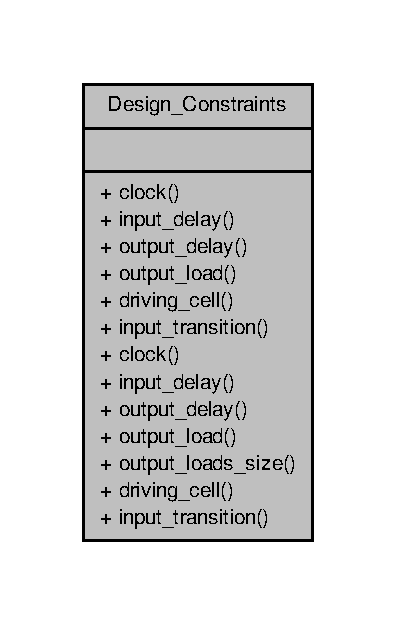
\includegraphics[width=190pt]{classDesign__Constraints__coll__graph}
\end{center}
\end{figure}
\subsection*{Public Member Functions}
\begin{DoxyCompactItemize}
\item 
void \hyperlink{classDesign__Constraints_a3d8381f421422cdaa12e78216a3b46a8}{clock} (const double clock)
\begin{DoxyCompactList}\small\item\em Sets clock period. frequency = 1 / clock\-\_\-period. \end{DoxyCompactList}\item 
bool \hyperlink{classDesign__Constraints_ab9e466f0f2ad7cfd16f8fe0d0b814b16}{input\-\_\-delay} (const string input\-\_\-name, const \hyperlink{classTransitions}{Transitions}$<$ double $>$ delay)
\begin{DoxyCompactList}\small\item\em Tries to set input delay. Returns true if succeeded. \end{DoxyCompactList}\item 
bool \hyperlink{classDesign__Constraints_a295b66d558e3aefea0b2d2629752517d}{output\-\_\-delay} (const string output\-\_\-name, const \hyperlink{classTransitions}{Transitions}$<$ double $>$ delay)
\begin{DoxyCompactList}\small\item\em Tries to set output delay. Returns true if succeeded. \end{DoxyCompactList}\item 
bool \hyperlink{classDesign__Constraints_a3a670a53112e18db745a6f3de9597cd3}{output\-\_\-load} (const string output\-\_\-name, const double output\-\_\-load)
\begin{DoxyCompactList}\small\item\em Tries to set output load. Returns true if succeeded. \end{DoxyCompactList}\item 
bool \hyperlink{classDesign__Constraints_a54c18f5ebd9dbcdc9d3ab8f2d363fc04}{driving\-\_\-cell} (const string input\-\_\-name, const string driving\-\_\-cell)
\begin{DoxyCompactList}\small\item\em Tries to set driving cell. Returns true if succeeded. \end{DoxyCompactList}\item 
bool \hyperlink{classDesign__Constraints_afd86c8844a5a62d1a6bbd7138d548cf9}{input\-\_\-transition} (const string input\-\_\-name, const \hyperlink{classTransitions}{Transitions}$<$ double $>$ transition)
\begin{DoxyCompactList}\small\item\em Tries to set input transitions. Returns true if succeeded. \end{DoxyCompactList}\item 
double \hyperlink{classDesign__Constraints_a535cc6d955b52c959b566510c1e3544a}{clock} () const 
\begin{DoxyCompactList}\small\item\em Returns clock period. \end{DoxyCompactList}\item 
const \hyperlink{classTransitions}{Transitions}$<$ double $>$ \hyperlink{classDesign__Constraints_ae67988a0cd0ba0ab5ad1463c273eb287}{input\-\_\-delay} (const string input\-\_\-name) const 
\begin{DoxyCompactList}\small\item\em Returns \hyperlink{classTransitions}{Transitions$<$double$>$} input\-\_\-delay with input\-\_\-name name. \end{DoxyCompactList}\item 
const \hyperlink{classTransitions}{Transitions}$<$ double $>$ \hyperlink{classDesign__Constraints_a07810050c6ae8a62d1e77ee23ad1f660}{output\-\_\-delay} (const string output\-\_\-name) const 
\begin{DoxyCompactList}\small\item\em Returns \hyperlink{classTransitions}{Transitions$<$double$>$} output\-\_\-delay with output\-\_\-name name. \end{DoxyCompactList}\item 
double \hyperlink{classDesign__Constraints_ab21387336a70852447a1d16e11358840}{output\-\_\-load} (const string output\-\_\-name) const 
\begin{DoxyCompactList}\small\item\em Returns output load with output\-\_\-name name. \end{DoxyCompactList}\item 
size\-\_\-t \hyperlink{classDesign__Constraints_a840bdfc3346651f9925ef35590f8c55b}{output\-\_\-loads\-\_\-size} () const 
\begin{DoxyCompactList}\small\item\em Returns output loads size. \end{DoxyCompactList}\item 
const string \hyperlink{classDesign__Constraints_a3155a41841b4c24e3f79e6e1a280d6df}{driving\-\_\-cell} (const string input\-\_\-name) const 
\begin{DoxyCompactList}\small\item\em Returns driving cell with input\-\_\-name name. \end{DoxyCompactList}\item 
const \hyperlink{classTransitions}{Transitions}$<$ double $>$ \hyperlink{classDesign__Constraints_a2fedb3b4d77d0b029e00bf0200fb84a2}{input\-\_\-transition} (const string input\-\_\-name) const 
\begin{DoxyCompactList}\small\item\em Returns Transition$<$double$>$ input\-\_\-transition with input\-\_\-name name. \end{DoxyCompactList}\end{DoxyCompactItemize}


\subsection{Detailed Description}
Represents the design constraints of the case in study. Generated by the \hyperlink{classSDCParser}{S\-D\-C\-Parser} class. 



\subsection{Member Function Documentation}
\hypertarget{classDesign__Constraints_a3d8381f421422cdaa12e78216a3b46a8}{\index{Design\-\_\-\-Constraints@{Design\-\_\-\-Constraints}!clock@{clock}}
\index{clock@{clock}!Design_Constraints@{Design\-\_\-\-Constraints}}
\subsubsection[{clock}]{\setlength{\rightskip}{0pt plus 5cm}void Design\-\_\-\-Constraints\-::clock (
\begin{DoxyParamCaption}
\item[{const double}]{clock}
\end{DoxyParamCaption}
)}}\label{classDesign__Constraints_a3d8381f421422cdaa12e78216a3b46a8}


Sets clock period. frequency = 1 / clock\-\_\-period. 

\begin{DoxyReturn}{Returns}
void 
\end{DoxyReturn}
\hypertarget{classDesign__Constraints_a535cc6d955b52c959b566510c1e3544a}{\index{Design\-\_\-\-Constraints@{Design\-\_\-\-Constraints}!clock@{clock}}
\index{clock@{clock}!Design_Constraints@{Design\-\_\-\-Constraints}}
\subsubsection[{clock}]{\setlength{\rightskip}{0pt plus 5cm}double Design\-\_\-\-Constraints\-::clock (
\begin{DoxyParamCaption}
{}
\end{DoxyParamCaption}
) const}}\label{classDesign__Constraints_a535cc6d955b52c959b566510c1e3544a}


Returns clock period. 

\begin{DoxyReturn}{Returns}
double 
\end{DoxyReturn}
\hypertarget{classDesign__Constraints_a54c18f5ebd9dbcdc9d3ab8f2d363fc04}{\index{Design\-\_\-\-Constraints@{Design\-\_\-\-Constraints}!driving\-\_\-cell@{driving\-\_\-cell}}
\index{driving\-\_\-cell@{driving\-\_\-cell}!Design_Constraints@{Design\-\_\-\-Constraints}}
\subsubsection[{driving\-\_\-cell}]{\setlength{\rightskip}{0pt plus 5cm}bool Design\-\_\-\-Constraints\-::driving\-\_\-cell (
\begin{DoxyParamCaption}
\item[{const string}]{input\-\_\-name, }
\item[{const string}]{driving\-\_\-cell}
\end{DoxyParamCaption}
)}}\label{classDesign__Constraints_a54c18f5ebd9dbcdc9d3ab8f2d363fc04}


Tries to set driving cell. Returns true if succeeded. 


\begin{DoxyParams}{Parameters}
{\em const} & string input\-\_\-name, const string driving\-\_\-cell\\
\hline
\end{DoxyParams}
\begin{DoxyReturn}{Returns}
bool 
\end{DoxyReturn}
\hypertarget{classDesign__Constraints_a3155a41841b4c24e3f79e6e1a280d6df}{\index{Design\-\_\-\-Constraints@{Design\-\_\-\-Constraints}!driving\-\_\-cell@{driving\-\_\-cell}}
\index{driving\-\_\-cell@{driving\-\_\-cell}!Design_Constraints@{Design\-\_\-\-Constraints}}
\subsubsection[{driving\-\_\-cell}]{\setlength{\rightskip}{0pt plus 5cm}const string Design\-\_\-\-Constraints\-::driving\-\_\-cell (
\begin{DoxyParamCaption}
\item[{const string}]{input\-\_\-name}
\end{DoxyParamCaption}
) const}}\label{classDesign__Constraints_a3155a41841b4c24e3f79e6e1a280d6df}


Returns driving cell with input\-\_\-name name. 


\begin{DoxyParams}{Parameters}
{\em const} & string input\-\_\-name\\
\hline
\end{DoxyParams}
\begin{DoxyReturn}{Returns}
const string 
\end{DoxyReturn}
\hypertarget{classDesign__Constraints_ab9e466f0f2ad7cfd16f8fe0d0b814b16}{\index{Design\-\_\-\-Constraints@{Design\-\_\-\-Constraints}!input\-\_\-delay@{input\-\_\-delay}}
\index{input\-\_\-delay@{input\-\_\-delay}!Design_Constraints@{Design\-\_\-\-Constraints}}
\subsubsection[{input\-\_\-delay}]{\setlength{\rightskip}{0pt plus 5cm}bool Design\-\_\-\-Constraints\-::input\-\_\-delay (
\begin{DoxyParamCaption}
\item[{const string}]{input\-\_\-name, }
\item[{const {\bf Transitions}$<$ double $>$}]{delay}
\end{DoxyParamCaption}
)}}\label{classDesign__Constraints_ab9e466f0f2ad7cfd16f8fe0d0b814b16}


Tries to set input delay. Returns true if succeeded. 


\begin{DoxyParams}{Parameters}
{\em const} & string input\-\_\-name, const \hyperlink{classTransitions}{Transitions$<$double$>$} delay\\
\hline
\end{DoxyParams}
\begin{DoxyReturn}{Returns}
bool 
\end{DoxyReturn}
\hypertarget{classDesign__Constraints_ae67988a0cd0ba0ab5ad1463c273eb287}{\index{Design\-\_\-\-Constraints@{Design\-\_\-\-Constraints}!input\-\_\-delay@{input\-\_\-delay}}
\index{input\-\_\-delay@{input\-\_\-delay}!Design_Constraints@{Design\-\_\-\-Constraints}}
\subsubsection[{input\-\_\-delay}]{\setlength{\rightskip}{0pt plus 5cm}const {\bf Transitions}$<$double$>$ Design\-\_\-\-Constraints\-::input\-\_\-delay (
\begin{DoxyParamCaption}
\item[{const string}]{input\-\_\-name}
\end{DoxyParamCaption}
) const}}\label{classDesign__Constraints_ae67988a0cd0ba0ab5ad1463c273eb287}


Returns \hyperlink{classTransitions}{Transitions$<$double$>$} input\-\_\-delay with input\-\_\-name name. 


\begin{DoxyParams}{Parameters}
{\em const} & string input\-\_\-name\\
\hline
\end{DoxyParams}
\begin{DoxyReturn}{Returns}
const \hyperlink{classTransitions}{Transitions$<$double$>$} 
\end{DoxyReturn}
\hypertarget{classDesign__Constraints_afd86c8844a5a62d1a6bbd7138d548cf9}{\index{Design\-\_\-\-Constraints@{Design\-\_\-\-Constraints}!input\-\_\-transition@{input\-\_\-transition}}
\index{input\-\_\-transition@{input\-\_\-transition}!Design_Constraints@{Design\-\_\-\-Constraints}}
\subsubsection[{input\-\_\-transition}]{\setlength{\rightskip}{0pt plus 5cm}bool Design\-\_\-\-Constraints\-::input\-\_\-transition (
\begin{DoxyParamCaption}
\item[{const string}]{input\-\_\-name, }
\item[{const {\bf Transitions}$<$ double $>$}]{transition}
\end{DoxyParamCaption}
)}}\label{classDesign__Constraints_afd86c8844a5a62d1a6bbd7138d548cf9}


Tries to set input transitions. Returns true if succeeded. 


\begin{DoxyParams}{Parameters}
{\em const} & string input\-\_\-name, const \hyperlink{classTransitions}{Transitions$<$double$>$} transition\\
\hline
\end{DoxyParams}
\begin{DoxyReturn}{Returns}
bool 
\end{DoxyReturn}
\hypertarget{classDesign__Constraints_a2fedb3b4d77d0b029e00bf0200fb84a2}{\index{Design\-\_\-\-Constraints@{Design\-\_\-\-Constraints}!input\-\_\-transition@{input\-\_\-transition}}
\index{input\-\_\-transition@{input\-\_\-transition}!Design_Constraints@{Design\-\_\-\-Constraints}}
\subsubsection[{input\-\_\-transition}]{\setlength{\rightskip}{0pt plus 5cm}const {\bf Transitions}$<$double$>$ Design\-\_\-\-Constraints\-::input\-\_\-transition (
\begin{DoxyParamCaption}
\item[{const string}]{input\-\_\-name}
\end{DoxyParamCaption}
) const}}\label{classDesign__Constraints_a2fedb3b4d77d0b029e00bf0200fb84a2}


Returns Transition$<$double$>$ input\-\_\-transition with input\-\_\-name name. 


\begin{DoxyParams}{Parameters}
{\em const} & string input\-\_\-name\\
\hline
\end{DoxyParams}
\begin{DoxyReturn}{Returns}
const Transition$<$double$>$ 
\end{DoxyReturn}
\hypertarget{classDesign__Constraints_a295b66d558e3aefea0b2d2629752517d}{\index{Design\-\_\-\-Constraints@{Design\-\_\-\-Constraints}!output\-\_\-delay@{output\-\_\-delay}}
\index{output\-\_\-delay@{output\-\_\-delay}!Design_Constraints@{Design\-\_\-\-Constraints}}
\subsubsection[{output\-\_\-delay}]{\setlength{\rightskip}{0pt plus 5cm}bool Design\-\_\-\-Constraints\-::output\-\_\-delay (
\begin{DoxyParamCaption}
\item[{const string}]{output\-\_\-name, }
\item[{const {\bf Transitions}$<$ double $>$}]{delay}
\end{DoxyParamCaption}
)}}\label{classDesign__Constraints_a295b66d558e3aefea0b2d2629752517d}


Tries to set output delay. Returns true if succeeded. 


\begin{DoxyParams}{Parameters}
{\em const} & string input\-\_\-name, const \hyperlink{classTransitions}{Transitions$<$double$>$} delay\\
\hline
\end{DoxyParams}
\begin{DoxyReturn}{Returns}
bool 
\end{DoxyReturn}
\hypertarget{classDesign__Constraints_a07810050c6ae8a62d1e77ee23ad1f660}{\index{Design\-\_\-\-Constraints@{Design\-\_\-\-Constraints}!output\-\_\-delay@{output\-\_\-delay}}
\index{output\-\_\-delay@{output\-\_\-delay}!Design_Constraints@{Design\-\_\-\-Constraints}}
\subsubsection[{output\-\_\-delay}]{\setlength{\rightskip}{0pt plus 5cm}const {\bf Transitions}$<$double$>$ Design\-\_\-\-Constraints\-::output\-\_\-delay (
\begin{DoxyParamCaption}
\item[{const string}]{output\-\_\-name}
\end{DoxyParamCaption}
) const}}\label{classDesign__Constraints_a07810050c6ae8a62d1e77ee23ad1f660}


Returns \hyperlink{classTransitions}{Transitions$<$double$>$} output\-\_\-delay with output\-\_\-name name. 


\begin{DoxyParams}{Parameters}
{\em const} & string output\-\_\-name\\
\hline
\end{DoxyParams}
\begin{DoxyReturn}{Returns}
const \hyperlink{classTransitions}{Transitions$<$double$>$} 
\end{DoxyReturn}
\hypertarget{classDesign__Constraints_a3a670a53112e18db745a6f3de9597cd3}{\index{Design\-\_\-\-Constraints@{Design\-\_\-\-Constraints}!output\-\_\-load@{output\-\_\-load}}
\index{output\-\_\-load@{output\-\_\-load}!Design_Constraints@{Design\-\_\-\-Constraints}}
\subsubsection[{output\-\_\-load}]{\setlength{\rightskip}{0pt plus 5cm}bool Design\-\_\-\-Constraints\-::output\-\_\-load (
\begin{DoxyParamCaption}
\item[{const string}]{output\-\_\-name, }
\item[{const double}]{output\-\_\-load}
\end{DoxyParamCaption}
)}}\label{classDesign__Constraints_a3a670a53112e18db745a6f3de9597cd3}


Tries to set output load. Returns true if succeeded. 


\begin{DoxyParams}{Parameters}
{\em const} & string input\-\_\-name, const \hyperlink{classTransitions}{Transitions$<$double$>$} output\-\_\-load\\
\hline
\end{DoxyParams}
\begin{DoxyReturn}{Returns}
bool 
\end{DoxyReturn}
\hypertarget{classDesign__Constraints_ab21387336a70852447a1d16e11358840}{\index{Design\-\_\-\-Constraints@{Design\-\_\-\-Constraints}!output\-\_\-load@{output\-\_\-load}}
\index{output\-\_\-load@{output\-\_\-load}!Design_Constraints@{Design\-\_\-\-Constraints}}
\subsubsection[{output\-\_\-load}]{\setlength{\rightskip}{0pt plus 5cm}double Design\-\_\-\-Constraints\-::output\-\_\-load (
\begin{DoxyParamCaption}
\item[{const string}]{output\-\_\-name}
\end{DoxyParamCaption}
) const}}\label{classDesign__Constraints_ab21387336a70852447a1d16e11358840}


Returns output load with output\-\_\-name name. 


\begin{DoxyParams}{Parameters}
{\em const} & string output\-\_\-name\\
\hline
\end{DoxyParams}
\begin{DoxyReturn}{Returns}
double 
\end{DoxyReturn}
\hypertarget{classDesign__Constraints_a840bdfc3346651f9925ef35590f8c55b}{\index{Design\-\_\-\-Constraints@{Design\-\_\-\-Constraints}!output\-\_\-loads\-\_\-size@{output\-\_\-loads\-\_\-size}}
\index{output\-\_\-loads\-\_\-size@{output\-\_\-loads\-\_\-size}!Design_Constraints@{Design\-\_\-\-Constraints}}
\subsubsection[{output\-\_\-loads\-\_\-size}]{\setlength{\rightskip}{0pt plus 5cm}size\-\_\-t Design\-\_\-\-Constraints\-::output\-\_\-loads\-\_\-size (
\begin{DoxyParamCaption}
{}
\end{DoxyParamCaption}
) const}}\label{classDesign__Constraints_a840bdfc3346651f9925ef35590f8c55b}


Returns output loads size. 

\begin{DoxyReturn}{Returns}
size\-\_\-t 
\end{DoxyReturn}


The documentation for this class was generated from the following file\-:\begin{DoxyCompactItemize}
\item 
Timing\-Analysis/src/include/\hyperlink{design__constraints_8h}{design\-\_\-constraints.\-h}\end{DoxyCompactItemize}

\hypertarget{classTiming__Analysis_1_1Edge}{\section{Timing\-\_\-\-Analysis\-:\-:Edge$<$ T $>$ Class Template Reference}
\label{classTiming__Analysis_1_1Edge}\index{Timing\-\_\-\-Analysis\-::\-Edge$<$ T $>$@{Timing\-\_\-\-Analysis\-::\-Edge$<$ T $>$}}
}


Template class which represents an edge of the graph model. An edge in graph theory is a connection between vertices.  




{\ttfamily \#include $<$edge.\-h$>$}

Inheritance diagram for Timing\-\_\-\-Analysis\-:\-:Edge$<$ T $>$\-:\begin{figure}[H]
\begin{center}
\leavevmode
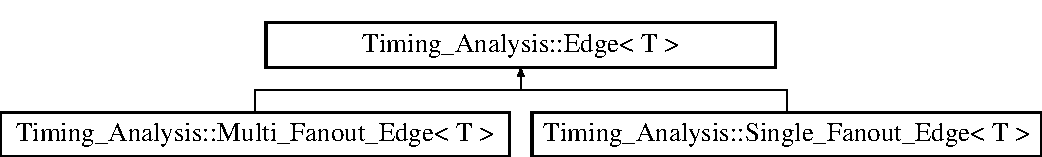
\includegraphics[height=2.000000cm]{classTiming__Analysis_1_1Edge}
\end{center}
\end{figure}
\subsection*{Public Member Functions}
\begin{DoxyCompactItemize}
\item 
T $\ast$ \hyperlink{classTiming__Analysis_1_1Edge_a47020ea89fd9fde438adc814a731a23d}{from} () const 
\begin{DoxyCompactList}\small\item\em Returns \-\_\-from$\ast$$\ast$$\ast$$\ast$$\ast$$\ast$$\ast$. \end{DoxyCompactList}\item 
size\-\_\-t \hyperlink{classTiming__Analysis_1_1Edge_a60c70172e973450774a8ec5d4dadbcb5}{fanouts\-\_\-size} () const 
\begin{DoxyCompactList}\small\item\em Returns fan out. \end{DoxyCompactList}\end{DoxyCompactItemize}
\subsection*{Protected Member Functions}
\begin{DoxyCompactItemize}
\item 
\hyperlink{classTiming__Analysis_1_1Edge_a64a07a7a08de0e2fd29b1d1db98c5d2d}{Edge} (T $\ast$\hyperlink{classTiming__Analysis_1_1Edge_a47020ea89fd9fde438adc814a731a23d}{from})
\begin{DoxyCompactList}\small\item\em \hyperlink{classTiming__Analysis_1_1Edge}{Edge} constructor. \end{DoxyCompactList}\item 
void \hyperlink{classTiming__Analysis_1_1Edge_a81bc4f5f07902385b2234bf591822a52}{set\-\_\-fanout} (const int i, T $\ast$tp)
\begin{DoxyCompactList}\small\item\em Inserts T pointer at index i. \end{DoxyCompactList}\item 
void \hyperlink{classTiming__Analysis_1_1Edge_ab9195f5c50f8a66b29f6856c9629fcc8}{add\-\_\-fanout} (T $\ast$tp)
\begin{DoxyCompactList}\small\item\em Inserts T pointer. \end{DoxyCompactList}\end{DoxyCompactItemize}
\subsection*{Protected Attributes}
\begin{DoxyCompactItemize}
\item 
\hypertarget{classTiming__Analysis_1_1Edge_a718ef7f37c4d9ddf867ef15eaa96ae43}{T $\ast$ {\bfseries \-\_\-from}}\label{classTiming__Analysis_1_1Edge_a718ef7f37c4d9ddf867ef15eaa96ae43}

\item 
\hypertarget{classTiming__Analysis_1_1Edge_ae1bc9c1f6a84a2b4a116d5c4571fba02}{vector$<$ T $\ast$ $>$ {\bfseries \-\_\-to}}\label{classTiming__Analysis_1_1Edge_ae1bc9c1f6a84a2b4a116d5c4571fba02}

\end{DoxyCompactItemize}


\subsection{Detailed Description}
\subsubsection*{template$<$typename T$>$class Timing\-\_\-\-Analysis\-::\-Edge$<$ T $>$}

Template class which represents an edge of the graph model. An edge in graph theory is a connection between vertices. 



\subsection{Constructor \& Destructor Documentation}
\hypertarget{classTiming__Analysis_1_1Edge_a64a07a7a08de0e2fd29b1d1db98c5d2d}{\index{Timing\-\_\-\-Analysis\-::\-Edge@{Timing\-\_\-\-Analysis\-::\-Edge}!Edge@{Edge}}
\index{Edge@{Edge}!Timing_Analysis::Edge@{Timing\-\_\-\-Analysis\-::\-Edge}}
\subsubsection[{Edge}]{\setlength{\rightskip}{0pt plus 5cm}template$<$typename T$>$ {\bf Timing\-\_\-\-Analysis\-::\-Edge}$<$ T $>$\-::{\bf Edge} (
\begin{DoxyParamCaption}
\item[{T $\ast$}]{from}
\end{DoxyParamCaption}
)\hspace{0.3cm}{\ttfamily [inline]}, {\ttfamily [protected]}}}\label{classTiming__Analysis_1_1Edge_a64a07a7a08de0e2fd29b1d1db98c5d2d}


\hyperlink{classTiming__Analysis_1_1Edge}{Edge} constructor. 


\begin{DoxyParams}{Parameters}
{\em T} & $\ast$ from \\
\hline
\end{DoxyParams}


\subsection{Member Function Documentation}
\hypertarget{classTiming__Analysis_1_1Edge_ab9195f5c50f8a66b29f6856c9629fcc8}{\index{Timing\-\_\-\-Analysis\-::\-Edge@{Timing\-\_\-\-Analysis\-::\-Edge}!add\-\_\-fanout@{add\-\_\-fanout}}
\index{add\-\_\-fanout@{add\-\_\-fanout}!Timing_Analysis::Edge@{Timing\-\_\-\-Analysis\-::\-Edge}}
\subsubsection[{add\-\_\-fanout}]{\setlength{\rightskip}{0pt plus 5cm}template$<$typename T$>$ void {\bf Timing\-\_\-\-Analysis\-::\-Edge}$<$ T $>$\-::add\-\_\-fanout (
\begin{DoxyParamCaption}
\item[{T $\ast$}]{tp}
\end{DoxyParamCaption}
)\hspace{0.3cm}{\ttfamily [inline]}, {\ttfamily [protected]}}}\label{classTiming__Analysis_1_1Edge_ab9195f5c50f8a66b29f6856c9629fcc8}


Inserts T pointer. 


\begin{DoxyParams}{Parameters}
{\em T} & $\ast$tp\\
\hline
\end{DoxyParams}
\begin{DoxyReturn}{Returns}
void 
\end{DoxyReturn}
\hypertarget{classTiming__Analysis_1_1Edge_a60c70172e973450774a8ec5d4dadbcb5}{\index{Timing\-\_\-\-Analysis\-::\-Edge@{Timing\-\_\-\-Analysis\-::\-Edge}!fanouts\-\_\-size@{fanouts\-\_\-size}}
\index{fanouts\-\_\-size@{fanouts\-\_\-size}!Timing_Analysis::Edge@{Timing\-\_\-\-Analysis\-::\-Edge}}
\subsubsection[{fanouts\-\_\-size}]{\setlength{\rightskip}{0pt plus 5cm}template$<$typename T$>$ size\-\_\-t {\bf Timing\-\_\-\-Analysis\-::\-Edge}$<$ T $>$\-::fanouts\-\_\-size (
\begin{DoxyParamCaption}
{}
\end{DoxyParamCaption}
) const\hspace{0.3cm}{\ttfamily [inline]}}}\label{classTiming__Analysis_1_1Edge_a60c70172e973450774a8ec5d4dadbcb5}


Returns fan out. 

\begin{DoxyReturn}{Returns}
size\-\_\-t 
\end{DoxyReturn}
\hypertarget{classTiming__Analysis_1_1Edge_a47020ea89fd9fde438adc814a731a23d}{\index{Timing\-\_\-\-Analysis\-::\-Edge@{Timing\-\_\-\-Analysis\-::\-Edge}!from@{from}}
\index{from@{from}!Timing_Analysis::Edge@{Timing\-\_\-\-Analysis\-::\-Edge}}
\subsubsection[{from}]{\setlength{\rightskip}{0pt plus 5cm}template$<$typename T$>$ T$\ast$ {\bf Timing\-\_\-\-Analysis\-::\-Edge}$<$ T $>$\-::from (
\begin{DoxyParamCaption}
{}
\end{DoxyParamCaption}
) const\hspace{0.3cm}{\ttfamily [inline]}}}\label{classTiming__Analysis_1_1Edge_a47020ea89fd9fde438adc814a731a23d}


Returns \-\_\-from$\ast$$\ast$$\ast$$\ast$$\ast$$\ast$$\ast$. 

\begin{DoxyReturn}{Returns}
T $\ast$ 
\end{DoxyReturn}
\hypertarget{classTiming__Analysis_1_1Edge_a81bc4f5f07902385b2234bf591822a52}{\index{Timing\-\_\-\-Analysis\-::\-Edge@{Timing\-\_\-\-Analysis\-::\-Edge}!set\-\_\-fanout@{set\-\_\-fanout}}
\index{set\-\_\-fanout@{set\-\_\-fanout}!Timing_Analysis::Edge@{Timing\-\_\-\-Analysis\-::\-Edge}}
\subsubsection[{set\-\_\-fanout}]{\setlength{\rightskip}{0pt plus 5cm}template$<$typename T$>$ void {\bf Timing\-\_\-\-Analysis\-::\-Edge}$<$ T $>$\-::set\-\_\-fanout (
\begin{DoxyParamCaption}
\item[{const int}]{i, }
\item[{T $\ast$}]{tp}
\end{DoxyParamCaption}
)\hspace{0.3cm}{\ttfamily [inline]}, {\ttfamily [protected]}}}\label{classTiming__Analysis_1_1Edge_a81bc4f5f07902385b2234bf591822a52}


Inserts T pointer at index i. 


\begin{DoxyParams}{Parameters}
{\em const} & int i, T $\ast$tp\\
\hline
\end{DoxyParams}
\begin{DoxyReturn}{Returns}
void 
\end{DoxyReturn}


The documentation for this class was generated from the following file\-:\begin{DoxyCompactItemize}
\item 
tcc\-Chrystian/src/include/edge.\-h\end{DoxyCompactItemize}

\hypertarget{structIF}{\section{I\-F$<$ cond, Then\-Type, Else\-Type $>$ Struct Template Reference}
\label{structIF}\index{I\-F$<$ cond, Then\-Type, Else\-Type $>$@{I\-F$<$ cond, Then\-Type, Else\-Type $>$}}
}


S\-T\-A\-T\-I\-C M\-E\-T\-A\-P\-R\-O\-G\-R\-A\-M\-M\-E\-D \hyperlink{structIF}{I\-F}.  




{\ttfamily \#include $<$configuration.\-h$>$}

\subsection*{Public Types}
\begin{DoxyCompactItemize}
\item 
\hypertarget{structIF_af93da5fd47eed555ff23c8d9022f8212}{typedef Then\-Type {\bfseries R\-E\-T}}\label{structIF_af93da5fd47eed555ff23c8d9022f8212}

\end{DoxyCompactItemize}


\subsection{Detailed Description}
\subsubsection*{template$<$bool cond, class Then\-Type, class Else\-Type$>$struct I\-F$<$ cond, Then\-Type, Else\-Type $>$}

S\-T\-A\-T\-I\-C M\-E\-T\-A\-P\-R\-O\-G\-R\-A\-M\-M\-E\-D \hyperlink{structIF}{I\-F}. 

This is a Configuration File To switch between I\-S\-P\-D2012 (Lumped Capacitance Wire Delay Model) or I\-S\-P\-D2013 (Distributed R\-C Wire Delay Model) S\-P\-E\-F format 

The documentation for this struct was generated from the following file\-:\begin{DoxyCompactItemize}
\item 
tcc\-Chrystian/src/include/configuration.\-h\end{DoxyCompactItemize}

\hypertarget{structIF_3_01false_00_01ThenType_00_01ElseType_01_4}{\section{I\-F$<$ false, Then\-Type, Else\-Type $>$ Struct Template Reference}
\label{structIF_3_01false_00_01ThenType_00_01ElseType_01_4}\index{I\-F$<$ false, Then\-Type, Else\-Type $>$@{I\-F$<$ false, Then\-Type, Else\-Type $>$}}
}


Metaprogrammed \hyperlink{structIF}{I\-F}.  




{\ttfamily \#include $<$configuration.\-h$>$}



Collaboration diagram for I\-F$<$ false, Then\-Type, Else\-Type $>$\-:\nopagebreak
\begin{figure}[H]
\begin{center}
\leavevmode
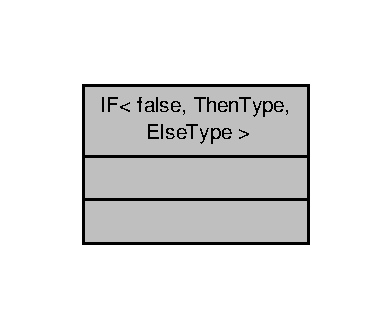
\includegraphics[width=188pt]{structIF_3_01false_00_01ThenType_00_01ElseType_01_4__coll__graph}
\end{center}
\end{figure}
\subsection*{Public Types}
\begin{DoxyCompactItemize}
\item 
typedef Else\-Type \hyperlink{structIF_3_01false_00_01ThenType_00_01ElseType_01_4_aa7d9ee5d71d3235a17de49470e2a00a0}{R\-E\-T}
\end{DoxyCompactItemize}


\subsection{Detailed Description}
\subsubsection*{template$<$class Then\-Type, class Else\-Type$>$struct I\-F$<$ false, Then\-Type, Else\-Type $>$}

Metaprogrammed \hyperlink{structIF}{I\-F}. 

\subsection{Member Typedef Documentation}
\hypertarget{structIF_3_01false_00_01ThenType_00_01ElseType_01_4_aa7d9ee5d71d3235a17de49470e2a00a0}{\index{I\-F$<$ false, Then\-Type, Else\-Type $>$@{I\-F$<$ false, Then\-Type, Else\-Type $>$}!R\-E\-T@{R\-E\-T}}
\index{R\-E\-T@{R\-E\-T}!IF< false, ThenType, ElseType >@{I\-F$<$ false, Then\-Type, Else\-Type $>$}}
\subsubsection[{R\-E\-T}]{\setlength{\rightskip}{0pt plus 5cm}template$<$class Then\-Type , class Else\-Type $>$ typedef Else\-Type {\bf I\-F}$<$ false, Then\-Type, Else\-Type $>$\-::{\bf R\-E\-T}}}\label{structIF_3_01false_00_01ThenType_00_01ElseType_01_4_aa7d9ee5d71d3235a17de49470e2a00a0}


The documentation for this struct was generated from the following file\-:\begin{DoxyCompactItemize}
\item 
Timing\-Analysis/src/include/\hyperlink{configuration_8h}{configuration.\-h}\end{DoxyCompactItemize}

\hypertarget{structLibertyCellInfo}{\section{Liberty\-Cell\-Info Struct Reference}
\label{structLibertyCellInfo}\index{Liberty\-Cell\-Info@{Liberty\-Cell\-Info}}
}
\subsection*{Public Member Functions}
\begin{DoxyCompactItemize}
\item 
\hyperlink{structLibertyCellInfo_a3250ab70b0c778ef0881b949c008814b}{Liberty\-Cell\-Info} ()
\begin{DoxyCompactList}\small\item\em \hyperlink{structLibertyCellInfo}{Liberty\-Cell\-Info} default constructor$\ast$$\ast$$\ast$$\ast$$\ast$$\ast$$\ast$$\ast$$\ast$$\ast$$\ast$. \end{DoxyCompactList}\end{DoxyCompactItemize}
\subsection*{Public Attributes}
\begin{DoxyCompactItemize}
\item 
\hypertarget{structLibertyCellInfo_a50066e7ef4d4110f6751bb9d81079614}{string {\bfseries name}}\label{structLibertyCellInfo_a50066e7ef4d4110f6751bb9d81079614}

\item 
\hypertarget{structLibertyCellInfo_af9b2d1f00a5d75b8e61bf3ce110a2d33}{string {\bfseries footprint}}\label{structLibertyCellInfo_af9b2d1f00a5d75b8e61bf3ce110a2d33}

\item 
\hypertarget{structLibertyCellInfo_a160c15b0dffa8079ec5bd52115f0d6cf}{double {\bfseries leakage\-Power}}\label{structLibertyCellInfo_a160c15b0dffa8079ec5bd52115f0d6cf}

\item 
\hypertarget{structLibertyCellInfo_a9fe14565c391db64fe59b885db703ba2}{double {\bfseries area}}\label{structLibertyCellInfo_a9fe14565c391db64fe59b885db703ba2}

\item 
\hypertarget{structLibertyCellInfo_a7d8643908315b2a90faf453fa475b2ea}{bool {\bfseries is\-Sequential}}\label{structLibertyCellInfo_a7d8643908315b2a90faf453fa475b2ea}

\item 
\hypertarget{structLibertyCellInfo_aad4eed91d5d0ecdda6ade0356ef8e5cf}{bool {\bfseries dont\-Touch}}\label{structLibertyCellInfo_aad4eed91d5d0ecdda6ade0356ef8e5cf}

\item 
\hypertarget{structLibertyCellInfo_a20420db0c6e78453236b10a62478f4e8}{bool {\bfseries primary\-Output}}\label{structLibertyCellInfo_a20420db0c6e78453236b10a62478f4e8}

\item 
\hypertarget{structLibertyCellInfo_a521bb57132e935e3a1db03227dc6345b}{vector$<$ \hyperlink{structLibertyPinInfo}{Liberty\-Pin\-Info} $>$ {\bfseries pins}}\label{structLibertyCellInfo_a521bb57132e935e3a1db03227dc6345b}

\item 
\hypertarget{structLibertyCellInfo_a28e5986b7cbdee33fbed50f4cb54c005}{vector$<$ \hyperlink{structLibertyTimingInfo}{Liberty\-Timing\-Info} $>$ {\bfseries timing\-Arcs}}\label{structLibertyCellInfo_a28e5986b7cbdee33fbed50f4cb54c005}

\end{DoxyCompactItemize}


\subsection{Constructor \& Destructor Documentation}
\hypertarget{structLibertyCellInfo_a3250ab70b0c778ef0881b949c008814b}{\index{Liberty\-Cell\-Info@{Liberty\-Cell\-Info}!Liberty\-Cell\-Info@{Liberty\-Cell\-Info}}
\index{Liberty\-Cell\-Info@{Liberty\-Cell\-Info}!LibertyCellInfo@{Liberty\-Cell\-Info}}
\subsubsection[{Liberty\-Cell\-Info}]{\setlength{\rightskip}{0pt plus 5cm}Liberty\-Cell\-Info\-::\-Liberty\-Cell\-Info (
\begin{DoxyParamCaption}
{}
\end{DoxyParamCaption}
)\hspace{0.3cm}{\ttfamily [inline]}}}\label{structLibertyCellInfo_a3250ab70b0c778ef0881b949c008814b}


\hyperlink{structLibertyCellInfo}{Liberty\-Cell\-Info} default constructor$\ast$$\ast$$\ast$$\ast$$\ast$$\ast$$\ast$$\ast$$\ast$$\ast$$\ast$. 



The documentation for this struct was generated from the following file\-:\begin{DoxyCompactItemize}
\item 
tcc\-Chrystian/src/include/liberty\-\_\-library.\-h\end{DoxyCompactItemize}

\hypertarget{classLibertyLibrary}{\section{Liberty\-Library Class Reference}
\label{classLibertyLibrary}\index{Liberty\-Library@{Liberty\-Library}}
}


Standard cell Library is a collection of logic functions info. Contains details about implementations of logic functions, within its layout, parasitic models, Verilog models, and more. Generated by the \hyperlink{classLibertyParser}{Liberty\-Parser} class.  




{\ttfamily \#include $<$liberty\-\_\-library.\-h$>$}



Collaboration diagram for Liberty\-Library\-:\nopagebreak
\begin{figure}[H]
\begin{center}
\leavevmode
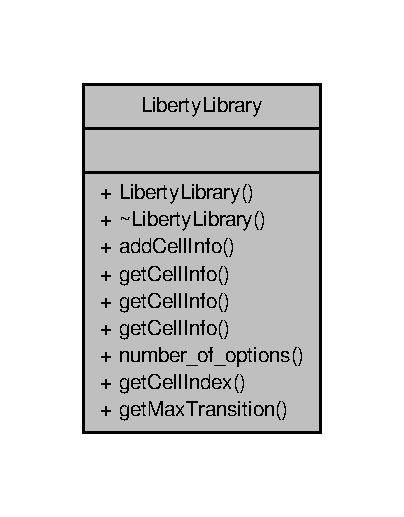
\includegraphics[width=194pt]{classLibertyLibrary__coll__graph}
\end{center}
\end{figure}
\subsection*{Public Member Functions}
\begin{DoxyCompactItemize}
\item 
\hyperlink{classLibertyLibrary_a3b7513ef68e791245f60e16f6b4ee5d4}{Liberty\-Library} (const double max\-Transition=0.\-0f)
\begin{DoxyCompactList}\small\item\em \hyperlink{classLibertyLibrary}{Liberty\-Library} default constructor. \end{DoxyCompactList}\item 
virtual \hyperlink{classLibertyLibrary_ade99b2247c7d5eb9ef885bc4ec57091d}{$\sim$\-Liberty\-Library} ()
\begin{DoxyCompactList}\small\item\em Empty \hyperlink{classLibertyLibrary}{Liberty\-Library} desctructor. \end{DoxyCompactList}\item 
const pair$<$ int, int $>$ \hyperlink{classLibertyLibrary_a4d9ec0ea6af3949878d9b14042e761e6}{add\-Cell\-Info} (const \hyperlink{structLibertyCellInfo}{Liberty\-Cell\-Info} \&cell\-Info)
\begin{DoxyCompactList}\small\item\em Returns pair$<$footprint index, option index$>$ \end{DoxyCompactList}\item 
const \hyperlink{structLibertyCellInfo}{Liberty\-Cell\-Info} \& \hyperlink{classLibertyLibrary_a917ae50f0af17b1b68be754f1ae6dd07}{get\-Cell\-Info} (const string \&foot\-Print, const int \&i) const 
\begin{DoxyCompactList}\small\item\em Returns \hyperlink{structLibertyCellInfo}{Liberty\-Cell\-Info} in foot\-Print, at index i. \end{DoxyCompactList}\item 
const \hyperlink{structLibertyCellInfo}{Liberty\-Cell\-Info} \& \hyperlink{classLibertyLibrary_a57c64ca6abd02f1e549eeb25178724c9}{get\-Cell\-Info} (const string \&cell\-Name) const 
\begin{DoxyCompactList}\small\item\em Returns \hyperlink{structLibertyCellInfo}{Liberty\-Cell\-Info} of cell\-Name name. \end{DoxyCompactList}\item 
const \hyperlink{structLibertyCellInfo}{Liberty\-Cell\-Info} \& \hyperlink{classLibertyLibrary_a227638e4b3a4b00faa659c45e20c0aaa}{get\-Cell\-Info} (const int \&foot\-Print\-Index, const int \&option\-Index) const 
\begin{DoxyCompactList}\small\item\em Returns \hyperlink{structLibertyCellInfo}{Liberty\-Cell\-Info} at index i, in foot\-Print of foot\-Print\-Index. \end{DoxyCompactList}\item 
size\-\_\-t \hyperlink{classLibertyLibrary_a411ffb8700a4dc393650ec341f33a2a7}{number\-\_\-of\-\_\-options} (const int footprint\-\_\-index) const 
\item 
const pair$<$ int, int $>$ \hyperlink{classLibertyLibrary_a08a8b3ab2b9e91574d1cdc39376839c8}{get\-Cell\-Index} (const string \&cell\-Name) const 
\begin{DoxyCompactList}\small\item\em Returns pair$<$footprint index, option index$>$ \end{DoxyCompactList}\item 
double \hyperlink{classLibertyLibrary_a954497f3bf2fe4ab640be24c23f976f4}{get\-Max\-Transition} () const 
\begin{DoxyCompactList}\small\item\em Returns max\-Transition. \end{DoxyCompactList}\end{DoxyCompactItemize}


\subsection{Detailed Description}
Standard cell Library is a collection of logic functions info. Contains details about implementations of logic functions, within its layout, parasitic models, Verilog models, and more. Generated by the \hyperlink{classLibertyParser}{Liberty\-Parser} class. 

\subsection{Constructor \& Destructor Documentation}
\hypertarget{classLibertyLibrary_a3b7513ef68e791245f60e16f6b4ee5d4}{\index{Liberty\-Library@{Liberty\-Library}!Liberty\-Library@{Liberty\-Library}}
\index{Liberty\-Library@{Liberty\-Library}!LibertyLibrary@{Liberty\-Library}}
\subsubsection[{Liberty\-Library}]{\setlength{\rightskip}{0pt plus 5cm}Liberty\-Library\-::\-Liberty\-Library (
\begin{DoxyParamCaption}
\item[{const double}]{max\-Transition = {\ttfamily 0.0f}}
\end{DoxyParamCaption}
)}}\label{classLibertyLibrary_a3b7513ef68e791245f60e16f6b4ee5d4}


\hyperlink{classLibertyLibrary}{Liberty\-Library} default constructor. 


\begin{DoxyParams}{Parameters}
{\em const} & double Max\-Transition \\
\hline
\end{DoxyParams}
\hypertarget{classLibertyLibrary_ade99b2247c7d5eb9ef885bc4ec57091d}{\index{Liberty\-Library@{Liberty\-Library}!$\sim$\-Liberty\-Library@{$\sim$\-Liberty\-Library}}
\index{$\sim$\-Liberty\-Library@{$\sim$\-Liberty\-Library}!LibertyLibrary@{Liberty\-Library}}
\subsubsection[{$\sim$\-Liberty\-Library}]{\setlength{\rightskip}{0pt plus 5cm}virtual Liberty\-Library\-::$\sim$\-Liberty\-Library (
\begin{DoxyParamCaption}
{}
\end{DoxyParamCaption}
)\hspace{0.3cm}{\ttfamily [virtual]}}}\label{classLibertyLibrary_ade99b2247c7d5eb9ef885bc4ec57091d}


Empty \hyperlink{classLibertyLibrary}{Liberty\-Library} desctructor. 



\subsection{Member Function Documentation}
\hypertarget{classLibertyLibrary_a4d9ec0ea6af3949878d9b14042e761e6}{\index{Liberty\-Library@{Liberty\-Library}!add\-Cell\-Info@{add\-Cell\-Info}}
\index{add\-Cell\-Info@{add\-Cell\-Info}!LibertyLibrary@{Liberty\-Library}}
\subsubsection[{add\-Cell\-Info}]{\setlength{\rightskip}{0pt plus 5cm}const pair$<$int, int$>$ Liberty\-Library\-::add\-Cell\-Info (
\begin{DoxyParamCaption}
\item[{const {\bf Liberty\-Cell\-Info} \&}]{cell\-Info}
\end{DoxyParamCaption}
)}}\label{classLibertyLibrary_a4d9ec0ea6af3949878d9b14042e761e6}


Returns pair$<$footprint index, option index$>$ 


\begin{DoxyParams}{Parameters}
{\em const} & \hyperlink{structLibertyCellInfo}{Liberty\-Cell\-Info} \& cell\-Info\\
\hline
\end{DoxyParams}
\begin{DoxyReturn}{Returns}
const pair$<$int, int$>$ 
\end{DoxyReturn}
\hypertarget{classLibertyLibrary_a08a8b3ab2b9e91574d1cdc39376839c8}{\index{Liberty\-Library@{Liberty\-Library}!get\-Cell\-Index@{get\-Cell\-Index}}
\index{get\-Cell\-Index@{get\-Cell\-Index}!LibertyLibrary@{Liberty\-Library}}
\subsubsection[{get\-Cell\-Index}]{\setlength{\rightskip}{0pt plus 5cm}const pair$<$int, int$>$ Liberty\-Library\-::get\-Cell\-Index (
\begin{DoxyParamCaption}
\item[{const string \&}]{cell\-Name}
\end{DoxyParamCaption}
) const}}\label{classLibertyLibrary_a08a8b3ab2b9e91574d1cdc39376839c8}


Returns pair$<$footprint index, option index$>$ 


\begin{DoxyParams}{Parameters}
{\em const} & string \&cell\-Name\\
\hline
\end{DoxyParams}
\begin{DoxyReturn}{Returns}
const pair$<$int, int$>$ 
\end{DoxyReturn}
\hypertarget{classLibertyLibrary_a917ae50f0af17b1b68be754f1ae6dd07}{\index{Liberty\-Library@{Liberty\-Library}!get\-Cell\-Info@{get\-Cell\-Info}}
\index{get\-Cell\-Info@{get\-Cell\-Info}!LibertyLibrary@{Liberty\-Library}}
\subsubsection[{get\-Cell\-Info}]{\setlength{\rightskip}{0pt plus 5cm}const {\bf Liberty\-Cell\-Info}\& Liberty\-Library\-::get\-Cell\-Info (
\begin{DoxyParamCaption}
\item[{const string \&}]{foot\-Print, }
\item[{const int \&}]{i}
\end{DoxyParamCaption}
) const}}\label{classLibertyLibrary_a917ae50f0af17b1b68be754f1ae6dd07}


Returns \hyperlink{structLibertyCellInfo}{Liberty\-Cell\-Info} in foot\-Print, at index i. 


\begin{DoxyParams}{Parameters}
{\em const} & string \& foot\-Print, const int \& i\\
\hline
\end{DoxyParams}
\begin{DoxyReturn}{Returns}
const \hyperlink{structLibertyCellInfo}{Liberty\-Cell\-Info} \& 
\end{DoxyReturn}
\hypertarget{classLibertyLibrary_a57c64ca6abd02f1e549eeb25178724c9}{\index{Liberty\-Library@{Liberty\-Library}!get\-Cell\-Info@{get\-Cell\-Info}}
\index{get\-Cell\-Info@{get\-Cell\-Info}!LibertyLibrary@{Liberty\-Library}}
\subsubsection[{get\-Cell\-Info}]{\setlength{\rightskip}{0pt plus 5cm}const {\bf Liberty\-Cell\-Info}\& Liberty\-Library\-::get\-Cell\-Info (
\begin{DoxyParamCaption}
\item[{const string \&}]{cell\-Name}
\end{DoxyParamCaption}
) const}}\label{classLibertyLibrary_a57c64ca6abd02f1e549eeb25178724c9}


Returns \hyperlink{structLibertyCellInfo}{Liberty\-Cell\-Info} of cell\-Name name. 


\begin{DoxyParams}{Parameters}
{\em const} & string \& cell\-Name\\
\hline
\end{DoxyParams}
\begin{DoxyReturn}{Returns}
const \hyperlink{structLibertyCellInfo}{Liberty\-Cell\-Info} \& 
\end{DoxyReturn}
\hypertarget{classLibertyLibrary_a227638e4b3a4b00faa659c45e20c0aaa}{\index{Liberty\-Library@{Liberty\-Library}!get\-Cell\-Info@{get\-Cell\-Info}}
\index{get\-Cell\-Info@{get\-Cell\-Info}!LibertyLibrary@{Liberty\-Library}}
\subsubsection[{get\-Cell\-Info}]{\setlength{\rightskip}{0pt plus 5cm}const {\bf Liberty\-Cell\-Info}\& Liberty\-Library\-::get\-Cell\-Info (
\begin{DoxyParamCaption}
\item[{const int \&}]{foot\-Print\-Index, }
\item[{const int \&}]{option\-Index}
\end{DoxyParamCaption}
) const}}\label{classLibertyLibrary_a227638e4b3a4b00faa659c45e20c0aaa}


Returns \hyperlink{structLibertyCellInfo}{Liberty\-Cell\-Info} at index i, in foot\-Print of foot\-Print\-Index. 


\begin{DoxyParams}{Parameters}
{\em const} & string \& foot\-Print\-Index, const int \& option\-Index\\
\hline
\end{DoxyParams}
\begin{DoxyReturn}{Returns}
const \hyperlink{structLibertyCellInfo}{Liberty\-Cell\-Info} \& 
\end{DoxyReturn}
\hypertarget{classLibertyLibrary_a954497f3bf2fe4ab640be24c23f976f4}{\index{Liberty\-Library@{Liberty\-Library}!get\-Max\-Transition@{get\-Max\-Transition}}
\index{get\-Max\-Transition@{get\-Max\-Transition}!LibertyLibrary@{Liberty\-Library}}
\subsubsection[{get\-Max\-Transition}]{\setlength{\rightskip}{0pt plus 5cm}double Liberty\-Library\-::get\-Max\-Transition (
\begin{DoxyParamCaption}
{}
\end{DoxyParamCaption}
) const}}\label{classLibertyLibrary_a954497f3bf2fe4ab640be24c23f976f4}


Returns max\-Transition. 

\begin{DoxyReturn}{Returns}
double 
\end{DoxyReturn}
\hypertarget{classLibertyLibrary_a411ffb8700a4dc393650ec341f33a2a7}{\index{Liberty\-Library@{Liberty\-Library}!number\-\_\-of\-\_\-options@{number\-\_\-of\-\_\-options}}
\index{number\-\_\-of\-\_\-options@{number\-\_\-of\-\_\-options}!LibertyLibrary@{Liberty\-Library}}
\subsubsection[{number\-\_\-of\-\_\-options}]{\setlength{\rightskip}{0pt plus 5cm}size\-\_\-t Liberty\-Library\-::number\-\_\-of\-\_\-options (
\begin{DoxyParamCaption}
\item[{const int}]{footprint\-\_\-index}
\end{DoxyParamCaption}
) const}}\label{classLibertyLibrary_a411ffb8700a4dc393650ec341f33a2a7}


The documentation for this class was generated from the following file\-:\begin{DoxyCompactItemize}
\item 
Timing\-Analysis/src/include/\hyperlink{liberty__library_8h}{liberty\-\_\-library.\-h}\end{DoxyCompactItemize}

\hypertarget{structLibertyLookupTable}{\section{Liberty\-Lookup\-Table Struct Reference}
\label{structLibertyLookupTable}\index{Liberty\-Lookup\-Table@{Liberty\-Lookup\-Table}}
}


Struct representing a lookup table to store delay or slew functions.  




{\ttfamily \#include $<$liberty\-\_\-library.\-h$>$}

\subsection*{Public Attributes}
\begin{DoxyCompactItemize}
\item 
\hypertarget{structLibertyLookupTable_aa9185452db835be3f9c603c3f3df5562}{vector$<$ double $>$ {\bfseries load\-Indices}}\label{structLibertyLookupTable_aa9185452db835be3f9c603c3f3df5562}

\item 
\hypertarget{structLibertyLookupTable_a1f7a1d2e84535f8c7df9bac33732634d}{vector$<$ double $>$ {\bfseries transition\-Indices}}\label{structLibertyLookupTable_a1f7a1d2e84535f8c7df9bac33732634d}

\item 
\hypertarget{structLibertyLookupTable_a1ca823f563ac9e3e8a616b09a19da596}{vector$<$ vector$<$ double $>$ $>$ {\bfseries table\-Vals}}\label{structLibertyLookupTable_a1ca823f563ac9e3e8a616b09a19da596}

\end{DoxyCompactItemize}


\subsection{Detailed Description}
Struct representing a lookup table to store delay or slew functions. 

Look up table is indexed by the output load and the input transition values

Let L = load\-Indices\mbox{[}i\mbox{]} T = transition\-Indices\mbox{[}j\mbox{]} Then, the table value corresponding to L and T will be\-: table\mbox{[}i\mbox{]}\mbox{[}j\mbox{]} 

The documentation for this struct was generated from the following file\-:\begin{DoxyCompactItemize}
\item 
tcc\-Chrystian/src/include/liberty\-\_\-library.\-h\end{DoxyCompactItemize}

\hypertarget{classLibertyLookupTableInterpolator}{\section{Liberty\-Lookup\-Table\-Interpolator Class Reference}
\label{classLibertyLookupTableInterpolator}\index{Liberty\-Lookup\-Table\-Interpolator@{Liberty\-Lookup\-Table\-Interpolator}}
}


Interpolation calculator.  




{\ttfamily \#include $<$liberty\-\_\-library.\-h$>$}

Inheritance diagram for Liberty\-Lookup\-Table\-Interpolator\-:\begin{figure}[H]
\begin{center}
\leavevmode
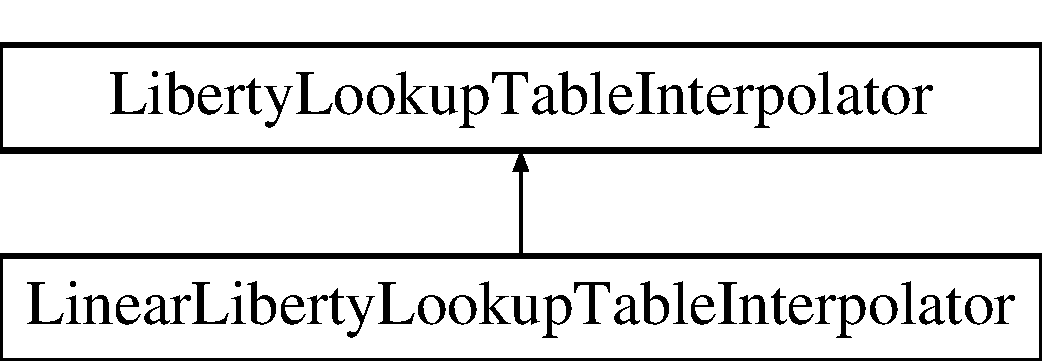
\includegraphics[height=2.000000cm]{classLibertyLookupTableInterpolator}
\end{center}
\end{figure}
\subsection*{Public Member Functions}
\begin{DoxyCompactItemize}
\item 
virtual double \hyperlink{classLibertyLookupTableInterpolator_ae12e0b9e427488bc933b54a427586f47}{interpolate} (const \hyperlink{structLibertyLookupTable}{Liberty\-Lookup\-Table} \&lut, const double load, const double transition)=0
\begin{DoxyCompactList}\small\item\em Returns interpolated value. \end{DoxyCompactList}\item 
virtual const \hyperlink{classTransitions}{Transitions}$<$ double $>$ \hyperlink{classLibertyLookupTableInterpolator_a3f840a4246b193e9e620b3ec8cadb720}{interpolate} (const \hyperlink{structLibertyLookupTable}{Liberty\-Lookup\-Table} \&rise\-Lut, const \hyperlink{structLibertyLookupTable}{Liberty\-Lookup\-Table} \&fall\-Lut, const \hyperlink{classTransitions}{Transitions}$<$ double $>$ load, const \hyperlink{classTransitions}{Transitions}$<$ double $>$ transition, Unateness unateness=N\-E\-G\-A\-T\-I\-V\-E\-\_\-\-U\-N\-A\-T\-E, bool is\-\_\-input\-\_\-driver=false)=0
\begin{DoxyCompactList}\small\item\em Returns Transitions$<$double, double$>$ with its rise and fall delay values interpolated. \end{DoxyCompactList}\end{DoxyCompactItemize}
\subsection*{Protected Member Functions}
\begin{DoxyCompactItemize}
\item 
void \hyperlink{classLibertyLookupTableInterpolator_a41f28d4091ef57ce488a26f0a3aedb0b}{round} (\hyperlink{classTransitions}{Transitions}$<$ double $>$ \&transitions, const int decimal\-\_\-places)
\begin{DoxyCompactList}\small\item\em Truncates \hyperlink{classTransitions}{Transitions$<$double$>$} to \hyperlink{classTransitions}{Transitions$<$double$>$} . Not implemented. \end{DoxyCompactList}\end{DoxyCompactItemize}
\subsection*{Static Protected Attributes}
\begin{DoxyCompactItemize}
\item 
\hypertarget{classLibertyLookupTableInterpolator_ad2d3a3313189ba7c9bb10dfbbef1a367}{static const int {\bfseries D\-E\-F\-A\-U\-L\-T\-\_\-\-D\-E\-C\-I\-M\-A\-L\-\_\-\-P\-L\-A\-C\-E\-S}}\label{classLibertyLookupTableInterpolator_ad2d3a3313189ba7c9bb10dfbbef1a367}

\end{DoxyCompactItemize}


\subsection{Detailed Description}
Interpolation calculator. 

\subsection{Member Function Documentation}
\hypertarget{classLibertyLookupTableInterpolator_ae12e0b9e427488bc933b54a427586f47}{\index{Liberty\-Lookup\-Table\-Interpolator@{Liberty\-Lookup\-Table\-Interpolator}!interpolate@{interpolate}}
\index{interpolate@{interpolate}!LibertyLookupTableInterpolator@{Liberty\-Lookup\-Table\-Interpolator}}
\subsubsection[{interpolate}]{\setlength{\rightskip}{0pt plus 5cm}virtual double Liberty\-Lookup\-Table\-Interpolator\-::interpolate (
\begin{DoxyParamCaption}
\item[{const {\bf Liberty\-Lookup\-Table} \&}]{lut, }
\item[{const double}]{load, }
\item[{const double}]{transition}
\end{DoxyParamCaption}
)\hspace{0.3cm}{\ttfamily [pure virtual]}}}\label{classLibertyLookupTableInterpolator_ae12e0b9e427488bc933b54a427586f47}


Returns interpolated value. 


\begin{DoxyParams}{Parameters}
{\em const} & \hyperlink{structLibertyLookupTable}{Liberty\-Lookup\-Table} \& lut, const double load, const double transition\\
\hline
\end{DoxyParams}
\begin{DoxyReturn}{Returns}
double 
\end{DoxyReturn}


Implemented in \hyperlink{classLinearLibertyLookupTableInterpolator_afd4bc7bfcf9e969478fbc9505b588bf3}{Linear\-Liberty\-Lookup\-Table\-Interpolator}.

\hypertarget{classLibertyLookupTableInterpolator_a3f840a4246b193e9e620b3ec8cadb720}{\index{Liberty\-Lookup\-Table\-Interpolator@{Liberty\-Lookup\-Table\-Interpolator}!interpolate@{interpolate}}
\index{interpolate@{interpolate}!LibertyLookupTableInterpolator@{Liberty\-Lookup\-Table\-Interpolator}}
\subsubsection[{interpolate}]{\setlength{\rightskip}{0pt plus 5cm}virtual const {\bf Transitions}$<$double$>$ Liberty\-Lookup\-Table\-Interpolator\-::interpolate (
\begin{DoxyParamCaption}
\item[{const {\bf Liberty\-Lookup\-Table} \&}]{rise\-Lut, }
\item[{const {\bf Liberty\-Lookup\-Table} \&}]{fall\-Lut, }
\item[{const {\bf Transitions}$<$ double $>$}]{load, }
\item[{const {\bf Transitions}$<$ double $>$}]{transition, }
\item[{Unateness}]{unateness = {\ttfamily NEGATIVE\-\_\-UNATE}, }
\item[{bool}]{is\-\_\-input\-\_\-driver = {\ttfamily false}}
\end{DoxyParamCaption}
)\hspace{0.3cm}{\ttfamily [pure virtual]}}}\label{classLibertyLookupTableInterpolator_a3f840a4246b193e9e620b3ec8cadb720}


Returns Transitions$<$double, double$>$ with its rise and fall delay values interpolated. 


\begin{DoxyParams}{Parameters}
{\em const} & \hyperlink{structLibertyLookupTable}{Liberty\-Lookup\-Table} \& rise\-Lut, const \hyperlink{structLibertyLookupTable}{Liberty\-Lookup\-Table} \& fall\-Lut, const \hyperlink{classTransitions}{Transitions$<$double$>$} load, const \hyperlink{classTransitions}{Transitions$<$double$>$} transition, Unateness unateness(default N\-E\-G\-A\-T\-I\-V\-E\-\_\-\-U\-N\-A\-T\-E), bool is\-\_\-input\-\_\-driver(default false)\\
\hline
\end{DoxyParams}
\begin{DoxyReturn}{Returns}
const \hyperlink{classTransitions}{Transitions$<$double$>$} 
\end{DoxyReturn}


Implemented in \hyperlink{classLinearLibertyLookupTableInterpolator_a9b0f96185327e7cb0e5c315691eb6579}{Linear\-Liberty\-Lookup\-Table\-Interpolator}.

\hypertarget{classLibertyLookupTableInterpolator_a41f28d4091ef57ce488a26f0a3aedb0b}{\index{Liberty\-Lookup\-Table\-Interpolator@{Liberty\-Lookup\-Table\-Interpolator}!round@{round}}
\index{round@{round}!LibertyLookupTableInterpolator@{Liberty\-Lookup\-Table\-Interpolator}}
\subsubsection[{round}]{\setlength{\rightskip}{0pt plus 5cm}void Liberty\-Lookup\-Table\-Interpolator\-::round (
\begin{DoxyParamCaption}
\item[{{\bf Transitions}$<$ double $>$ \&}]{transitions, }
\item[{const int}]{decimal\-\_\-places}
\end{DoxyParamCaption}
)\hspace{0.3cm}{\ttfamily [protected]}}}\label{classLibertyLookupTableInterpolator_a41f28d4091ef57ce488a26f0a3aedb0b}


Truncates \hyperlink{classTransitions}{Transitions$<$double$>$} to \hyperlink{classTransitions}{Transitions$<$double$>$} . Not implemented. 


\begin{DoxyParams}{Parameters}
{\em \hyperlink{classTransitions}{Transitions$<$double$>$}} & \& transitions, const int decimal\-\_\-places\\
\hline
\end{DoxyParams}
\begin{DoxyReturn}{Returns}
void 
\end{DoxyReturn}


The documentation for this class was generated from the following file\-:\begin{DoxyCompactItemize}
\item 
tcc\-Chrystian/src/include/liberty\-\_\-library.\-h\end{DoxyCompactItemize}

\hypertarget{classLibertyParser}{\section{Liberty\-Parser Class Reference}
\label{classLibertyParser}\index{Liberty\-Parser@{Liberty\-Parser}}
}


Inherits from \hyperlink{classParser}{Parser}. Used to generate a \hyperlink{classLibertyLibrary}{Liberty\-Library} object from a file.  




{\ttfamily \#include $<$parser.\-h$>$}



Inheritance diagram for Liberty\-Parser\-:\nopagebreak
\begin{figure}[H]
\begin{center}
\leavevmode
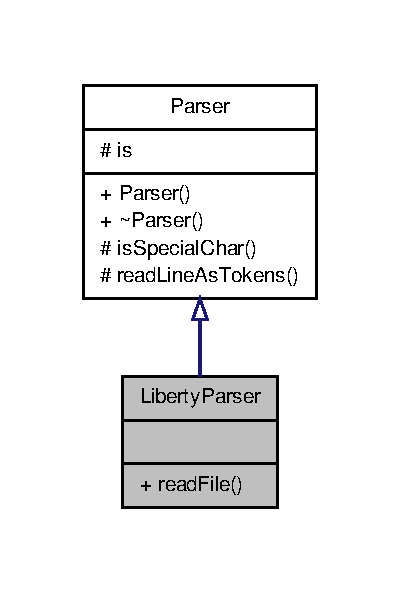
\includegraphics[width=192pt]{classLibertyParser__inherit__graph}
\end{center}
\end{figure}


Collaboration diagram for Liberty\-Parser\-:\nopagebreak
\begin{figure}[H]
\begin{center}
\leavevmode
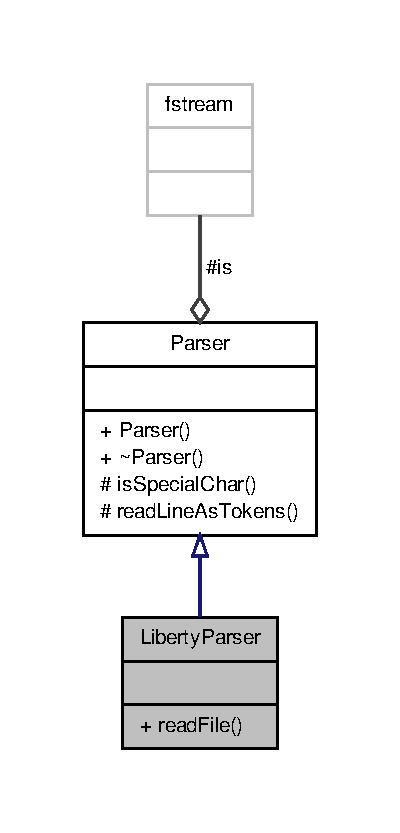
\includegraphics[width=192pt]{classLibertyParser__coll__graph}
\end{center}
\end{figure}
\subsection*{Public Member Functions}
\begin{DoxyCompactItemize}
\item 
const \hyperlink{classLibertyLibrary}{Liberty\-Library} \hyperlink{classLibertyParser_a474451e29a86949f6ebef6948363874d}{read\-File} (const string filename)
\begin{DoxyCompactList}\small\item\em Returns \hyperlink{classLibertyLibrary}{Liberty\-Library} generated using values read from file passed as filename parameter. \end{DoxyCompactList}\end{DoxyCompactItemize}
\subsection*{Additional Inherited Members}


\subsection{Detailed Description}
Inherits from \hyperlink{classParser}{Parser}. Used to generate a \hyperlink{classLibertyLibrary}{Liberty\-Library} object from a file. 

\begin{DoxyRemark}{Remarks}
See test\-\_\-lib\-\_\-parser () function in parser\-\_\-helper.\-cpp for an example of how to use this class. 
\end{DoxyRemark}


\subsection{Member Function Documentation}
\hypertarget{classLibertyParser_a474451e29a86949f6ebef6948363874d}{\index{Liberty\-Parser@{Liberty\-Parser}!read\-File@{read\-File}}
\index{read\-File@{read\-File}!LibertyParser@{Liberty\-Parser}}
\subsubsection[{read\-File}]{\setlength{\rightskip}{0pt plus 5cm}const {\bf Liberty\-Library} Liberty\-Parser\-::read\-File (
\begin{DoxyParamCaption}
\item[{const string}]{filename}
\end{DoxyParamCaption}
)}}\label{classLibertyParser_a474451e29a86949f6ebef6948363874d}


Returns \hyperlink{classLibertyLibrary}{Liberty\-Library} generated using values read from file passed as filename parameter. 


\begin{DoxyParams}{Parameters}
{\em const} & string filename\\
\hline
\end{DoxyParams}
\begin{DoxyReturn}{Returns}
Liberty\-Livrary 
\end{DoxyReturn}


The documentation for this class was generated from the following file\-:\begin{DoxyCompactItemize}
\item 
Timing\-Analysis/src/include/\hyperlink{parser_8h}{parser.\-h}\end{DoxyCompactItemize}

\hypertarget{structLibertyPinInfo}{\section{Liberty\-Pin\-Info Struct Reference}
\label{structLibertyPinInfo}\index{Liberty\-Pin\-Info@{Liberty\-Pin\-Info}}
}


Struct which has informations about a pin.  




{\ttfamily \#include $<$liberty\-\_\-library.\-h$>$}

\subsection*{Public Member Functions}
\begin{DoxyCompactItemize}
\item 
\hypertarget{structLibertyPinInfo_a268a64137463b6b6fdc87ed036184e45}{\hyperlink{structLibertyPinInfo_a268a64137463b6b6fdc87ed036184e45}{Liberty\-Pin\-Info} ()}\label{structLibertyPinInfo_a268a64137463b6b6fdc87ed036184e45}

\begin{DoxyCompactList}\small\item\em \hyperlink{structLibertyPinInfo}{Liberty\-Pin\-Info} default constructor. \end{DoxyCompactList}\end{DoxyCompactItemize}
\subsection*{Public Attributes}
\begin{DoxyCompactItemize}
\item 
\hypertarget{structLibertyPinInfo_a4421a56d0603f0d8371a48c123832aed}{string {\bfseries name}}\label{structLibertyPinInfo_a4421a56d0603f0d8371a48c123832aed}

\item 
\hypertarget{structLibertyPinInfo_a8668778fc79c36a4cdcedf9a3f7e91b4}{double {\bfseries capacitance}}\label{structLibertyPinInfo_a8668778fc79c36a4cdcedf9a3f7e91b4}

\item 
\hypertarget{structLibertyPinInfo_a8eb7d3102925e3ecf9906ade7c82b0b7}{double {\bfseries max\-Capacitance}}\label{structLibertyPinInfo_a8eb7d3102925e3ecf9906ade7c82b0b7}

\item 
\hypertarget{structLibertyPinInfo_a57daad21ecac17f40631e0c563f7f39d}{bool {\bfseries is\-Input}}\label{structLibertyPinInfo_a57daad21ecac17f40631e0c563f7f39d}

\item 
\hypertarget{structLibertyPinInfo_a8200642f454380e2e22f4158d471c302}{bool {\bfseries is\-Clock}}\label{structLibertyPinInfo_a8200642f454380e2e22f4158d471c302}

\end{DoxyCompactItemize}


\subsection{Detailed Description}
Struct which has informations about a pin. 

The documentation for this struct was generated from the following file\-:\begin{DoxyCompactItemize}
\item 
tcc\-Chrystian/src/include/liberty\-\_\-library.\-h\end{DoxyCompactItemize}

\hypertarget{structLibertyTimingInfo}{\section{Liberty\-Timing\-Info Struct Reference}
\label{structLibertyTimingInfo}\index{Liberty\-Timing\-Info@{Liberty\-Timing\-Info}}
}
\subsection*{Public Attributes}
\begin{DoxyCompactItemize}
\item 
\hypertarget{structLibertyTimingInfo_a6cb3b02b8c016a6a0f633ade7a8ee499}{string {\bfseries from\-Pin}}\label{structLibertyTimingInfo_a6cb3b02b8c016a6a0f633ade7a8ee499}

\item 
\hypertarget{structLibertyTimingInfo_a2bc2b4f64c8a8b71e314b97a37f14db4}{string {\bfseries to\-Pin}}\label{structLibertyTimingInfo_a2bc2b4f64c8a8b71e314b97a37f14db4}

\item 
\hypertarget{structLibertyTimingInfo_a54b164af0fb48cdbceb754858cbeface}{string {\bfseries timing\-Sense}}\label{structLibertyTimingInfo_a54b164af0fb48cdbceb754858cbeface}

\item 
\hypertarget{structLibertyTimingInfo_a4fdd676db9841962ef570a064ff97c81}{timing model for I\-S\-P\-D \\*
\hyperlink{structLibertyLookupTable}{Liberty\-Lookup\-Table} \hyperlink{structLibertyTimingInfo_a4fdd676db9841962ef570a064ff97c81}{fall\-Delay}}\label{structLibertyTimingInfo_a4fdd676db9841962ef570a064ff97c81}

\begin{DoxyCompactList}\small\item\em \char`\"{}non\-\_\-unate\char`\"{} or \char`\"{}negative\-\_\-unate\char`\"{} or \char`\"{}positive\-\_\-unate\char`\"{}. Note that I\-S\-P\-D-\/13 library will have only negative-\/unate combinational cells. The clock arcs for sequentials will be non\-\_\-unate (which can be ignored because of the simplified sequential \end{DoxyCompactList}\item 
\hypertarget{structLibertyTimingInfo_af2baf3e8053ed178d0d3dc8159ab8248}{\hyperlink{structLibertyLookupTable}{Liberty\-Lookup\-Table} {\bfseries rise\-Delay}}\label{structLibertyTimingInfo_af2baf3e8053ed178d0d3dc8159ab8248}

\item 
\hypertarget{structLibertyTimingInfo_a5af7b44ccbb69224084557182d2e3acb}{\hyperlink{structLibertyLookupTable}{Liberty\-Lookup\-Table} {\bfseries fall\-Transition}}\label{structLibertyTimingInfo_a5af7b44ccbb69224084557182d2e3acb}

\item 
\hypertarget{structLibertyTimingInfo_a1b31e1e18c0cc373e1eeaa1e999fbedd}{\hyperlink{structLibertyLookupTable}{Liberty\-Lookup\-Table} {\bfseries rise\-Transition}}\label{structLibertyTimingInfo_a1b31e1e18c0cc373e1eeaa1e999fbedd}

\end{DoxyCompactItemize}


The documentation for this struct was generated from the following file\-:\begin{DoxyCompactItemize}
\item 
tcc\-Chrystian/src/include/liberty\-\_\-library.\-h\end{DoxyCompactItemize}

\hypertarget{classLinearLibertyLookupTableInterpolator}{\section{Linear\-Liberty\-Lookup\-Table\-Interpolator Class Reference}
\label{classLinearLibertyLookupTableInterpolator}\index{Linear\-Liberty\-Lookup\-Table\-Interpolator@{Linear\-Liberty\-Lookup\-Table\-Interpolator}}
}
Inheritance diagram for Linear\-Liberty\-Lookup\-Table\-Interpolator\-:\begin{figure}[H]
\begin{center}
\leavevmode
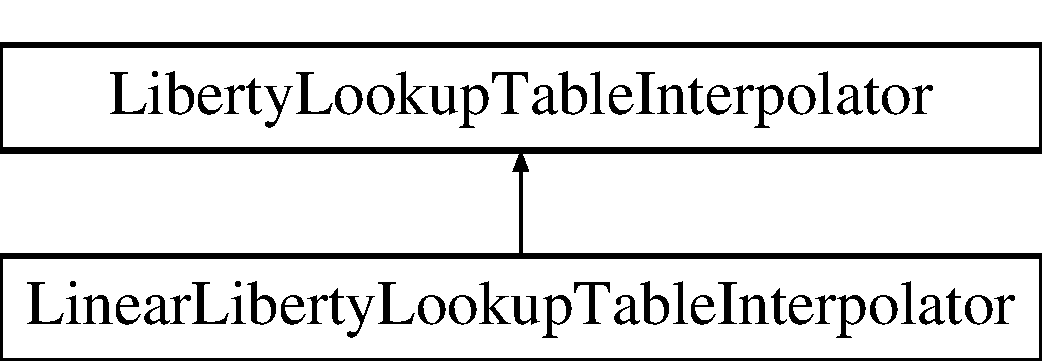
\includegraphics[height=2.000000cm]{classLinearLibertyLookupTableInterpolator}
\end{center}
\end{figure}
\subsection*{Public Member Functions}
\begin{DoxyCompactItemize}
\item 
double \hyperlink{classLinearLibertyLookupTableInterpolator_afd4bc7bfcf9e969478fbc9505b588bf3}{interpolate} (const \hyperlink{structLibertyLookupTable}{Liberty\-Lookup\-Table} \&lut, const double load, const double transition)
\begin{DoxyCompactList}\small\item\em Returns interpolation of L\-U\-T. \end{DoxyCompactList}\item 
const \hyperlink{classTransitions}{Transitions}$<$ double $>$ \hyperlink{classLinearLibertyLookupTableInterpolator_a9b0f96185327e7cb0e5c315691eb6579}{interpolate} (const \hyperlink{structLibertyLookupTable}{Liberty\-Lookup\-Table} \&rise\-Lut, const \hyperlink{structLibertyLookupTable}{Liberty\-Lookup\-Table} \&fall\-Lut, const \hyperlink{classTransitions}{Transitions}$<$ double $>$ load, const \hyperlink{classTransitions}{Transitions}$<$ double $>$ transition, Unateness unateness=N\-E\-G\-A\-T\-I\-V\-E\-\_\-\-U\-N\-A\-T\-E, bool is\-\_\-input\-\_\-driver=false)
\begin{DoxyCompactList}\small\item\em Returns interpolation of L\-U\-T$\ast$$\ast$$\ast$$\ast$$\ast$$\ast$$\ast$$\ast$$\ast$$\ast$$\ast$$\ast$$\ast$$\ast$$\ast$$\ast$$\ast$$\ast$$\ast$. \end{DoxyCompactList}\end{DoxyCompactItemize}
\subsection*{Additional Inherited Members}


\subsection{Member Function Documentation}
\hypertarget{classLinearLibertyLookupTableInterpolator_afd4bc7bfcf9e969478fbc9505b588bf3}{\index{Linear\-Liberty\-Lookup\-Table\-Interpolator@{Linear\-Liberty\-Lookup\-Table\-Interpolator}!interpolate@{interpolate}}
\index{interpolate@{interpolate}!LinearLibertyLookupTableInterpolator@{Linear\-Liberty\-Lookup\-Table\-Interpolator}}
\subsubsection[{interpolate}]{\setlength{\rightskip}{0pt plus 5cm}double Linear\-Liberty\-Lookup\-Table\-Interpolator\-::interpolate (
\begin{DoxyParamCaption}
\item[{const {\bf Liberty\-Lookup\-Table} \&}]{lut, }
\item[{const double}]{load, }
\item[{const double}]{transition}
\end{DoxyParamCaption}
)\hspace{0.3cm}{\ttfamily [virtual]}}}\label{classLinearLibertyLookupTableInterpolator_afd4bc7bfcf9e969478fbc9505b588bf3}


Returns interpolation of L\-U\-T. 


\begin{DoxyParams}{Parameters}
{\em const} & \hyperlink{structLibertyLookupTable}{Liberty\-Lookup\-Table} \& lut, const double load, const double transition\\
\hline
\end{DoxyParams}
\begin{DoxyReturn}{Returns}
double 
\end{DoxyReturn}


Implements \hyperlink{classLibertyLookupTableInterpolator_ae12e0b9e427488bc933b54a427586f47}{Liberty\-Lookup\-Table\-Interpolator}.

\hypertarget{classLinearLibertyLookupTableInterpolator_a9b0f96185327e7cb0e5c315691eb6579}{\index{Linear\-Liberty\-Lookup\-Table\-Interpolator@{Linear\-Liberty\-Lookup\-Table\-Interpolator}!interpolate@{interpolate}}
\index{interpolate@{interpolate}!LinearLibertyLookupTableInterpolator@{Linear\-Liberty\-Lookup\-Table\-Interpolator}}
\subsubsection[{interpolate}]{\setlength{\rightskip}{0pt plus 5cm}const {\bf Transitions}$<$double$>$ Linear\-Liberty\-Lookup\-Table\-Interpolator\-::interpolate (
\begin{DoxyParamCaption}
\item[{const {\bf Liberty\-Lookup\-Table} \&}]{rise\-Lut, }
\item[{const {\bf Liberty\-Lookup\-Table} \&}]{fall\-Lut, }
\item[{const {\bf Transitions}$<$ double $>$}]{load, }
\item[{const {\bf Transitions}$<$ double $>$}]{transition, }
\item[{Unateness}]{unateness = {\ttfamily NEGATIVE\-\_\-UNATE}, }
\item[{bool}]{is\-\_\-input\-\_\-driver = {\ttfamily false}}
\end{DoxyParamCaption}
)\hspace{0.3cm}{\ttfamily [virtual]}}}\label{classLinearLibertyLookupTableInterpolator_a9b0f96185327e7cb0e5c315691eb6579}


Returns interpolation of L\-U\-T$\ast$$\ast$$\ast$$\ast$$\ast$$\ast$$\ast$$\ast$$\ast$$\ast$$\ast$$\ast$$\ast$$\ast$$\ast$$\ast$$\ast$$\ast$$\ast$. 


\begin{DoxyParams}{Parameters}
{\em const} & \hyperlink{structLibertyLookupTable}{Liberty\-Lookup\-Table} \& rise\-Lut, const \hyperlink{structLibertyLookupTable}{Liberty\-Lookup\-Table} \& fall\-Lut, const \hyperlink{classTransitions}{Transitions$<$double$>$} load, const \hyperlink{classTransitions}{Transitions$<$double$>$} transition, Unateness unateness(default N\-E\-G\-A\-T\-I\-V\-E\-\_\-\-U\-N\-A\-T\-E), bool is\-\_\-input\-\_\-driver(default false)\\
\hline
\end{DoxyParams}
\begin{DoxyReturn}{Returns}
const \hyperlink{classTransitions}{Transitions$<$double$>$} 
\end{DoxyReturn}


Implements \hyperlink{classLibertyLookupTableInterpolator_a3f840a4246b193e9e620b3ec8cadb720}{Liberty\-Lookup\-Table\-Interpolator}.



The documentation for this class was generated from the following file\-:\begin{DoxyCompactItemize}
\item 
tcc\-Chrystian/src/include/liberty\-\_\-library.\-h\end{DoxyCompactItemize}

\hypertarget{structCircuit__Netlist_1_1Logic__Gate}{\section{Circuit\-\_\-\-Netlist\-:\-:Logic\-\_\-\-Gate Struct Reference}
\label{structCircuit__Netlist_1_1Logic__Gate}\index{Circuit\-\_\-\-Netlist\-::\-Logic\-\_\-\-Gate@{Circuit\-\_\-\-Netlist\-::\-Logic\-\_\-\-Gate}}
}


Struct which represents a \hyperlink{structCircuit__Netlist_1_1Logic__Gate}{Logic\-\_\-\-Gate}.  




{\ttfamily \#include $<$circuit\-\_\-netlist.\-h$>$}



Collaboration diagram for Circuit\-\_\-\-Netlist\-:\-:Logic\-\_\-\-Gate\-:\nopagebreak
\begin{figure}[H]
\begin{center}
\leavevmode
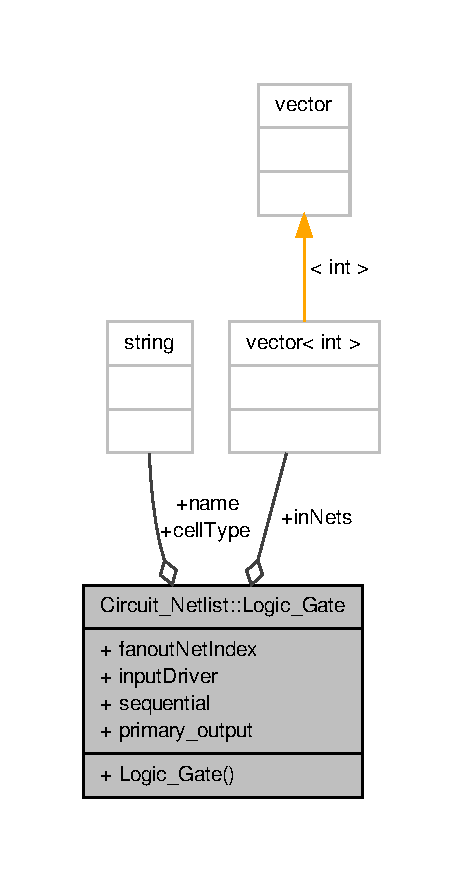
\includegraphics[width=222pt]{structCircuit__Netlist_1_1Logic__Gate__coll__graph}
\end{center}
\end{figure}
\subsection*{Public Member Functions}
\begin{DoxyCompactItemize}
\item 
\hyperlink{structCircuit__Netlist_1_1Logic__Gate_a81569a5c27c575b1725c5da2c2090f54}{Logic\-\_\-\-Gate} (const string \hyperlink{structCircuit__Netlist_1_1Logic__Gate_aa780fa4baf5244fcf34c52053005f73a}{name}, const string \hyperlink{structCircuit__Netlist_1_1Logic__Gate_a3b48b229126233bf5a98f39b003e7e5a}{cell\-Type}, const unsigned inputs, int \hyperlink{structCircuit__Netlist_1_1Logic__Gate_ac77535e3e3fff92529fa21d711cd0487}{fanout\-Net\-Index}, const bool \hyperlink{structCircuit__Netlist_1_1Logic__Gate_ad08611514342cd0293640fac9eebc61a}{input\-Driver}=false, const bool \hyperlink{structCircuit__Netlist_1_1Logic__Gate_a475c5b2598538600935f66be43c163fa}{primary\-\_\-output}=false)
\begin{DoxyCompactList}\small\item\em \hyperlink{structCircuit__Netlist_1_1Logic__Gate}{Logic\-\_\-\-Gate} constructor. \end{DoxyCompactList}\end{DoxyCompactItemize}
\subsection*{Public Attributes}
\begin{DoxyCompactItemize}
\item 
string \hyperlink{structCircuit__Netlist_1_1Logic__Gate_aa780fa4baf5244fcf34c52053005f73a}{name}
\item 
string \hyperlink{structCircuit__Netlist_1_1Logic__Gate_a3b48b229126233bf5a98f39b003e7e5a}{cell\-Type}
\item 
vector$<$ int $>$ \hyperlink{structCircuit__Netlist_1_1Logic__Gate_a0ada4f530d1846973daed17e35eb10a7}{in\-Nets}
\item 
int \hyperlink{structCircuit__Netlist_1_1Logic__Gate_ac77535e3e3fff92529fa21d711cd0487}{fanout\-Net\-Index}
\item 
bool \hyperlink{structCircuit__Netlist_1_1Logic__Gate_ad08611514342cd0293640fac9eebc61a}{input\-Driver}
\item 
bool \hyperlink{structCircuit__Netlist_1_1Logic__Gate_a3919c593d1a40b4467d6735be783eee6}{sequential}
\item 
bool \hyperlink{structCircuit__Netlist_1_1Logic__Gate_a475c5b2598538600935f66be43c163fa}{primary\-\_\-output}
\end{DoxyCompactItemize}


\subsection{Detailed Description}
Struct which represents a \hyperlink{structCircuit__Netlist_1_1Logic__Gate}{Logic\-\_\-\-Gate}. 



\subsection{Constructor \& Destructor Documentation}
\hypertarget{structCircuit__Netlist_1_1Logic__Gate_a81569a5c27c575b1725c5da2c2090f54}{\index{Circuit\-\_\-\-Netlist\-::\-Logic\-\_\-\-Gate@{Circuit\-\_\-\-Netlist\-::\-Logic\-\_\-\-Gate}!Logic\-\_\-\-Gate@{Logic\-\_\-\-Gate}}
\index{Logic\-\_\-\-Gate@{Logic\-\_\-\-Gate}!Circuit_Netlist::Logic_Gate@{Circuit\-\_\-\-Netlist\-::\-Logic\-\_\-\-Gate}}
\subsubsection[{Logic\-\_\-\-Gate}]{\setlength{\rightskip}{0pt plus 5cm}Circuit\-\_\-\-Netlist\-::\-Logic\-\_\-\-Gate\-::\-Logic\-\_\-\-Gate (
\begin{DoxyParamCaption}
\item[{const string}]{name, }
\item[{const string}]{cell\-Type, }
\item[{const unsigned}]{inputs, }
\item[{int}]{fanout\-Net\-Index, }
\item[{const bool}]{input\-Driver = {\ttfamily false}, }
\item[{const bool}]{primary\-\_\-output = {\ttfamily false}}
\end{DoxyParamCaption}
)\hspace{0.3cm}{\ttfamily [inline]}}}\label{structCircuit__Netlist_1_1Logic__Gate_a81569a5c27c575b1725c5da2c2090f54}


\hyperlink{structCircuit__Netlist_1_1Logic__Gate}{Logic\-\_\-\-Gate} constructor. 


\begin{DoxyParams}{Parameters}
{\em const} & string name, const string cell\-Type, const unsigned inputs, int fanout\-Net\-Index, const bool input\-Driver(false default), const bool primary\-\_\-output(false default) \\
\hline
\end{DoxyParams}


\subsection{Member Data Documentation}
\hypertarget{structCircuit__Netlist_1_1Logic__Gate_a3b48b229126233bf5a98f39b003e7e5a}{\index{Circuit\-\_\-\-Netlist\-::\-Logic\-\_\-\-Gate@{Circuit\-\_\-\-Netlist\-::\-Logic\-\_\-\-Gate}!cell\-Type@{cell\-Type}}
\index{cell\-Type@{cell\-Type}!Circuit_Netlist::Logic_Gate@{Circuit\-\_\-\-Netlist\-::\-Logic\-\_\-\-Gate}}
\subsubsection[{cell\-Type}]{\setlength{\rightskip}{0pt plus 5cm}string Circuit\-\_\-\-Netlist\-::\-Logic\-\_\-\-Gate\-::cell\-Type}}\label{structCircuit__Netlist_1_1Logic__Gate_a3b48b229126233bf5a98f39b003e7e5a}
\hypertarget{structCircuit__Netlist_1_1Logic__Gate_ac77535e3e3fff92529fa21d711cd0487}{\index{Circuit\-\_\-\-Netlist\-::\-Logic\-\_\-\-Gate@{Circuit\-\_\-\-Netlist\-::\-Logic\-\_\-\-Gate}!fanout\-Net\-Index@{fanout\-Net\-Index}}
\index{fanout\-Net\-Index@{fanout\-Net\-Index}!Circuit_Netlist::Logic_Gate@{Circuit\-\_\-\-Netlist\-::\-Logic\-\_\-\-Gate}}
\subsubsection[{fanout\-Net\-Index}]{\setlength{\rightskip}{0pt plus 5cm}int Circuit\-\_\-\-Netlist\-::\-Logic\-\_\-\-Gate\-::fanout\-Net\-Index}}\label{structCircuit__Netlist_1_1Logic__Gate_ac77535e3e3fff92529fa21d711cd0487}
\hypertarget{structCircuit__Netlist_1_1Logic__Gate_a0ada4f530d1846973daed17e35eb10a7}{\index{Circuit\-\_\-\-Netlist\-::\-Logic\-\_\-\-Gate@{Circuit\-\_\-\-Netlist\-::\-Logic\-\_\-\-Gate}!in\-Nets@{in\-Nets}}
\index{in\-Nets@{in\-Nets}!Circuit_Netlist::Logic_Gate@{Circuit\-\_\-\-Netlist\-::\-Logic\-\_\-\-Gate}}
\subsubsection[{in\-Nets}]{\setlength{\rightskip}{0pt plus 5cm}vector$<$int$>$ Circuit\-\_\-\-Netlist\-::\-Logic\-\_\-\-Gate\-::in\-Nets}}\label{structCircuit__Netlist_1_1Logic__Gate_a0ada4f530d1846973daed17e35eb10a7}
\hypertarget{structCircuit__Netlist_1_1Logic__Gate_ad08611514342cd0293640fac9eebc61a}{\index{Circuit\-\_\-\-Netlist\-::\-Logic\-\_\-\-Gate@{Circuit\-\_\-\-Netlist\-::\-Logic\-\_\-\-Gate}!input\-Driver@{input\-Driver}}
\index{input\-Driver@{input\-Driver}!Circuit_Netlist::Logic_Gate@{Circuit\-\_\-\-Netlist\-::\-Logic\-\_\-\-Gate}}
\subsubsection[{input\-Driver}]{\setlength{\rightskip}{0pt plus 5cm}bool Circuit\-\_\-\-Netlist\-::\-Logic\-\_\-\-Gate\-::input\-Driver}}\label{structCircuit__Netlist_1_1Logic__Gate_ad08611514342cd0293640fac9eebc61a}
\hypertarget{structCircuit__Netlist_1_1Logic__Gate_aa780fa4baf5244fcf34c52053005f73a}{\index{Circuit\-\_\-\-Netlist\-::\-Logic\-\_\-\-Gate@{Circuit\-\_\-\-Netlist\-::\-Logic\-\_\-\-Gate}!name@{name}}
\index{name@{name}!Circuit_Netlist::Logic_Gate@{Circuit\-\_\-\-Netlist\-::\-Logic\-\_\-\-Gate}}
\subsubsection[{name}]{\setlength{\rightskip}{0pt plus 5cm}string Circuit\-\_\-\-Netlist\-::\-Logic\-\_\-\-Gate\-::name}}\label{structCircuit__Netlist_1_1Logic__Gate_aa780fa4baf5244fcf34c52053005f73a}
\hypertarget{structCircuit__Netlist_1_1Logic__Gate_a475c5b2598538600935f66be43c163fa}{\index{Circuit\-\_\-\-Netlist\-::\-Logic\-\_\-\-Gate@{Circuit\-\_\-\-Netlist\-::\-Logic\-\_\-\-Gate}!primary\-\_\-output@{primary\-\_\-output}}
\index{primary\-\_\-output@{primary\-\_\-output}!Circuit_Netlist::Logic_Gate@{Circuit\-\_\-\-Netlist\-::\-Logic\-\_\-\-Gate}}
\subsubsection[{primary\-\_\-output}]{\setlength{\rightskip}{0pt plus 5cm}bool Circuit\-\_\-\-Netlist\-::\-Logic\-\_\-\-Gate\-::primary\-\_\-output}}\label{structCircuit__Netlist_1_1Logic__Gate_a475c5b2598538600935f66be43c163fa}
\hypertarget{structCircuit__Netlist_1_1Logic__Gate_a3919c593d1a40b4467d6735be783eee6}{\index{Circuit\-\_\-\-Netlist\-::\-Logic\-\_\-\-Gate@{Circuit\-\_\-\-Netlist\-::\-Logic\-\_\-\-Gate}!sequential@{sequential}}
\index{sequential@{sequential}!Circuit_Netlist::Logic_Gate@{Circuit\-\_\-\-Netlist\-::\-Logic\-\_\-\-Gate}}
\subsubsection[{sequential}]{\setlength{\rightskip}{0pt plus 5cm}bool Circuit\-\_\-\-Netlist\-::\-Logic\-\_\-\-Gate\-::sequential}}\label{structCircuit__Netlist_1_1Logic__Gate_a3919c593d1a40b4467d6735be783eee6}


The documentation for this struct was generated from the following file\-:\begin{DoxyCompactItemize}
\item 
Timing\-Analysis/src/include/\hyperlink{circuit__netlist_8h}{circuit\-\_\-netlist.\-h}\end{DoxyCompactItemize}

\hypertarget{classLumpedCapacitanceWireDelayModel}{\section{Lumped\-Capacitance\-Wire\-Delay\-Model Class Reference}
\label{classLumpedCapacitanceWireDelayModel}\index{Lumped\-Capacitance\-Wire\-Delay\-Model@{Lumped\-Capacitance\-Wire\-Delay\-Model}}
}


Describes the Lumped Capacitance Model.  




{\ttfamily \#include $<$wire\-\_\-delay\-\_\-model.\-h$>$}

Inheritance diagram for Lumped\-Capacitance\-Wire\-Delay\-Model\-:\begin{figure}[H]
\begin{center}
\leavevmode
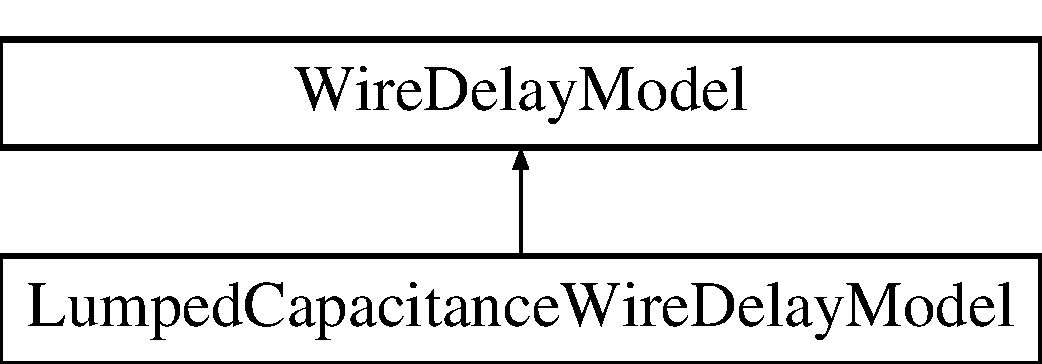
\includegraphics[height=2.000000cm]{classLumpedCapacitanceWireDelayModel}
\end{center}
\end{figure}
\subsection*{Public Member Functions}
\begin{DoxyCompactItemize}
\item 
\hypertarget{classLumpedCapacitanceWireDelayModel_ae147cdba517e3f6152ed8234473e5443}{{\bfseries Lumped\-Capacitance\-Wire\-Delay\-Model} (const Spef\-Net \&descriptor, const string root\-\_\-node, const bool dummy\-\_\-edge=false)}\label{classLumpedCapacitanceWireDelayModel_ae147cdba517e3f6152ed8234473e5443}

\item 
const \hyperlink{classTransitions}{Transitions}$<$ double $>$ \hyperlink{classLumpedCapacitanceWireDelayModel_a1bba0aef3bebe8df97a63e05b307b19a}{simulate} (const \hyperlink{structLibertyCellInfo}{Liberty\-Cell\-Info} \&cell\-Info, const int input, const \hyperlink{classTransitions}{Transitions}$<$ double $>$ \-\_\-slew, bool is\-\_\-input\-\_\-driver)
\item 
const \hyperlink{classTransitions}{Transitions}$<$ double $>$ \hyperlink{classLumpedCapacitanceWireDelayModel_a0266cb676908d95bdfcb64d1137898b0}{delay\-\_\-at\-\_\-fanout\-\_\-node} (const string fanout\-\_\-node\-\_\-name) const 
\begin{DoxyCompactList}\small\item\em Returns \hyperlink{classTransitions}{Transitions} with rise and fall delay time values set to zero. \end{DoxyCompactList}\item 
const \hyperlink{classTransitions}{Transitions}$<$ double $>$ \hyperlink{classLumpedCapacitanceWireDelayModel_aaedd69e811e7220e48493c51fb0443ed}{slew\-\_\-at\-\_\-fanout\-\_\-node} (const string fanout\-\_\-node\-\_\-name) const 
\begin{DoxyCompactList}\small\item\em Returns \hyperlink{classTransitions}{Transitions} with rise and fall slew time values set to zero. \end{DoxyCompactList}\item 
void \hyperlink{classLumpedCapacitanceWireDelayModel_a888f7e6a4951837072b937ae30e93073}{set\-Fanout\-Pin\-Capacitance} (const string fanout\-\_\-name\-\_\-and\-\_\-pin, const double pin\-Capacitance)
\begin{DoxyCompactList}\small\item\em Increments lumped capacitance of the wire. \end{DoxyCompactList}\item 
\hyperlink{classTransitions}{Transitions}$<$ double $>$ \hyperlink{classLumpedCapacitanceWireDelayModel_ab090355a74a21b5d6008352ff2a7d137}{root\-\_\-delay} (int arc\-\_\-number)
\begin{DoxyCompactList}\small\item\em not yet implemented$\ast$$\ast$$\ast$$\ast$$\ast$$\ast$$\ast$$\ast$$\ast$$\ast$$\ast$$\ast$$\ast$$\ast$$\ast$$\ast$$\ast$$\ast$$\ast$$\ast$$\ast$$\ast$$\ast$ \end{DoxyCompactList}\item 
\hyperlink{classTransitions}{Transitions}$<$ double $>$ \hyperlink{classLumpedCapacitanceWireDelayModel_a65e4141bbf97638c2334f71dfbf0ccfd}{root\-\_\-slew} (int arc\-\_\-number)
\begin{DoxyCompactList}\small\item\em not yet implemented$\ast$$\ast$$\ast$$\ast$$\ast$$\ast$$\ast$$\ast$$\ast$$\ast$$\ast$$\ast$$\ast$$\ast$$\ast$$\ast$$\ast$$\ast$$\ast$$\ast$$\ast$$\ast$$\ast$ \end{DoxyCompactList}\item 
void \hyperlink{classLumpedCapacitanceWireDelayModel_acca0415a76729b616be06543262ef441}{clear} ()
\begin{DoxyCompactList}\small\item\em not yet implemented$\ast$$\ast$$\ast$$\ast$$\ast$$\ast$$\ast$$\ast$$\ast$$\ast$$\ast$$\ast$$\ast$$\ast$$\ast$$\ast$$\ast$$\ast$$\ast$$\ast$$\ast$$\ast$ \end{DoxyCompactList}\end{DoxyCompactItemize}
\subsection*{Additional Inherited Members}


\subsection{Detailed Description}
Describes the Lumped Capacitance Model. 

\subsection{Member Function Documentation}
\hypertarget{classLumpedCapacitanceWireDelayModel_acca0415a76729b616be06543262ef441}{\index{Lumped\-Capacitance\-Wire\-Delay\-Model@{Lumped\-Capacitance\-Wire\-Delay\-Model}!clear@{clear}}
\index{clear@{clear}!LumpedCapacitanceWireDelayModel@{Lumped\-Capacitance\-Wire\-Delay\-Model}}
\subsubsection[{clear}]{\setlength{\rightskip}{0pt plus 5cm}void Lumped\-Capacitance\-Wire\-Delay\-Model\-::clear (
\begin{DoxyParamCaption}
{}
\end{DoxyParamCaption}
)\hspace{0.3cm}{\ttfamily [virtual]}}}\label{classLumpedCapacitanceWireDelayModel_acca0415a76729b616be06543262ef441}


not yet implemented$\ast$$\ast$$\ast$$\ast$$\ast$$\ast$$\ast$$\ast$$\ast$$\ast$$\ast$$\ast$$\ast$$\ast$$\ast$$\ast$$\ast$$\ast$$\ast$$\ast$$\ast$$\ast$ 

\begin{DoxyReturn}{Returns}
void 
\end{DoxyReturn}


Implements \hyperlink{classWireDelayModel_a74869a3a66deb53507e8bc6f16eff45c}{Wire\-Delay\-Model}.

\hypertarget{classLumpedCapacitanceWireDelayModel_a0266cb676908d95bdfcb64d1137898b0}{\index{Lumped\-Capacitance\-Wire\-Delay\-Model@{Lumped\-Capacitance\-Wire\-Delay\-Model}!delay\-\_\-at\-\_\-fanout\-\_\-node@{delay\-\_\-at\-\_\-fanout\-\_\-node}}
\index{delay\-\_\-at\-\_\-fanout\-\_\-node@{delay\-\_\-at\-\_\-fanout\-\_\-node}!LumpedCapacitanceWireDelayModel@{Lumped\-Capacitance\-Wire\-Delay\-Model}}
\subsubsection[{delay\-\_\-at\-\_\-fanout\-\_\-node}]{\setlength{\rightskip}{0pt plus 5cm}const {\bf Transitions}$<$double$>$ Lumped\-Capacitance\-Wire\-Delay\-Model\-::delay\-\_\-at\-\_\-fanout\-\_\-node (
\begin{DoxyParamCaption}
\item[{const string}]{fanout\-\_\-node\-\_\-name}
\end{DoxyParamCaption}
) const\hspace{0.3cm}{\ttfamily [virtual]}}}\label{classLumpedCapacitanceWireDelayModel_a0266cb676908d95bdfcb64d1137898b0}


Returns \hyperlink{classTransitions}{Transitions} with rise and fall delay time values set to zero. 


\begin{DoxyParams}{Parameters}
{\em const} & string fanout\-\_\-node\-\_\-name\\
\hline
\end{DoxyParams}
\begin{DoxyReturn}{Returns}
\hyperlink{classTransitions}{Transitions$<$double$>$} 
\end{DoxyReturn}


Implements \hyperlink{classWireDelayModel_a45a83dd192bcbf2a70ee13899256fe0d}{Wire\-Delay\-Model}.

\hypertarget{classLumpedCapacitanceWireDelayModel_ab090355a74a21b5d6008352ff2a7d137}{\index{Lumped\-Capacitance\-Wire\-Delay\-Model@{Lumped\-Capacitance\-Wire\-Delay\-Model}!root\-\_\-delay@{root\-\_\-delay}}
\index{root\-\_\-delay@{root\-\_\-delay}!LumpedCapacitanceWireDelayModel@{Lumped\-Capacitance\-Wire\-Delay\-Model}}
\subsubsection[{root\-\_\-delay}]{\setlength{\rightskip}{0pt plus 5cm}{\bf Transitions}$<$double$>$ Lumped\-Capacitance\-Wire\-Delay\-Model\-::root\-\_\-delay (
\begin{DoxyParamCaption}
\item[{int}]{arc\-\_\-number}
\end{DoxyParamCaption}
)\hspace{0.3cm}{\ttfamily [virtual]}}}\label{classLumpedCapacitanceWireDelayModel_ab090355a74a21b5d6008352ff2a7d137}


not yet implemented$\ast$$\ast$$\ast$$\ast$$\ast$$\ast$$\ast$$\ast$$\ast$$\ast$$\ast$$\ast$$\ast$$\ast$$\ast$$\ast$$\ast$$\ast$$\ast$$\ast$$\ast$$\ast$$\ast$ 


\begin{DoxyParams}{Parameters}
{\em int} & arc\-\_\-number\\
\hline
\end{DoxyParams}
\begin{DoxyReturn}{Returns}
\hyperlink{classTransitions}{Transitions$<$double$>$} 
\end{DoxyReturn}


Implements \hyperlink{classWireDelayModel_a4f4ab93810af8ad90fd9fca0b06de141}{Wire\-Delay\-Model}.

\hypertarget{classLumpedCapacitanceWireDelayModel_a65e4141bbf97638c2334f71dfbf0ccfd}{\index{Lumped\-Capacitance\-Wire\-Delay\-Model@{Lumped\-Capacitance\-Wire\-Delay\-Model}!root\-\_\-slew@{root\-\_\-slew}}
\index{root\-\_\-slew@{root\-\_\-slew}!LumpedCapacitanceWireDelayModel@{Lumped\-Capacitance\-Wire\-Delay\-Model}}
\subsubsection[{root\-\_\-slew}]{\setlength{\rightskip}{0pt plus 5cm}{\bf Transitions}$<$double$>$ Lumped\-Capacitance\-Wire\-Delay\-Model\-::root\-\_\-slew (
\begin{DoxyParamCaption}
\item[{int}]{arc\-\_\-number}
\end{DoxyParamCaption}
)\hspace{0.3cm}{\ttfamily [virtual]}}}\label{classLumpedCapacitanceWireDelayModel_a65e4141bbf97638c2334f71dfbf0ccfd}


not yet implemented$\ast$$\ast$$\ast$$\ast$$\ast$$\ast$$\ast$$\ast$$\ast$$\ast$$\ast$$\ast$$\ast$$\ast$$\ast$$\ast$$\ast$$\ast$$\ast$$\ast$$\ast$$\ast$$\ast$ 


\begin{DoxyParams}{Parameters}
{\em int} & arc\-\_\-number\\
\hline
\end{DoxyParams}
\begin{DoxyReturn}{Returns}
\hyperlink{classTransitions}{Transitions$<$double$>$} 
\end{DoxyReturn}


Implements \hyperlink{classWireDelayModel_a9e5344c26b73f549a2b5c38fea8af13d}{Wire\-Delay\-Model}.

\hypertarget{classLumpedCapacitanceWireDelayModel_a888f7e6a4951837072b937ae30e93073}{\index{Lumped\-Capacitance\-Wire\-Delay\-Model@{Lumped\-Capacitance\-Wire\-Delay\-Model}!set\-Fanout\-Pin\-Capacitance@{set\-Fanout\-Pin\-Capacitance}}
\index{set\-Fanout\-Pin\-Capacitance@{set\-Fanout\-Pin\-Capacitance}!LumpedCapacitanceWireDelayModel@{Lumped\-Capacitance\-Wire\-Delay\-Model}}
\subsubsection[{set\-Fanout\-Pin\-Capacitance}]{\setlength{\rightskip}{0pt plus 5cm}void Lumped\-Capacitance\-Wire\-Delay\-Model\-::set\-Fanout\-Pin\-Capacitance (
\begin{DoxyParamCaption}
\item[{const string}]{fanout\-Name\-And\-Pin, }
\item[{const double}]{pin\-Capacitance}
\end{DoxyParamCaption}
)\hspace{0.3cm}{\ttfamily [inline]}, {\ttfamily [virtual]}}}\label{classLumpedCapacitanceWireDelayModel_a888f7e6a4951837072b937ae30e93073}


Increments lumped capacitance of the wire. 


\begin{DoxyParams}{Parameters}
{\em const} & string fanout\-Name\-And\-Pin, const double capacitance\\
\hline
\end{DoxyParams}
\begin{DoxyReturn}{Returns}
void 
\end{DoxyReturn}


Implements \hyperlink{classWireDelayModel_a27d557bc1f2ed7e5e9787a8a5d82ecb2}{Wire\-Delay\-Model}.

\hypertarget{classLumpedCapacitanceWireDelayModel_a1bba0aef3bebe8df97a63e05b307b19a}{\index{Lumped\-Capacitance\-Wire\-Delay\-Model@{Lumped\-Capacitance\-Wire\-Delay\-Model}!simulate@{simulate}}
\index{simulate@{simulate}!LumpedCapacitanceWireDelayModel@{Lumped\-Capacitance\-Wire\-Delay\-Model}}
\subsubsection[{simulate}]{\setlength{\rightskip}{0pt plus 5cm}const {\bf Transitions}$<$double$>$ Lumped\-Capacitance\-Wire\-Delay\-Model\-::simulate (
\begin{DoxyParamCaption}
\item[{const {\bf Liberty\-Cell\-Info} \&}]{cell\-Info, }
\item[{const int}]{input, }
\item[{const {\bf Transitions}$<$ double $>$}]{slew, }
\item[{bool}]{is\-\_\-input\-\_\-driver}
\end{DoxyParamCaption}
)\hspace{0.3cm}{\ttfamily [virtual]}}}\label{classLumpedCapacitanceWireDelayModel_a1bba0aef3bebe8df97a63e05b307b19a}

\begin{DoxyParams}{Parameters}
{\em const} & \hyperlink{structLibertyCellInfo}{Liberty\-Cell\-Info} \& cell\-Info, const int input, const \hyperlink{classTransitions}{Transitions$<$double$>$} slew, bool is\-\_\-input\-\_\-driver\\
\hline
\end{DoxyParams}
\begin{DoxyReturn}{Returns}
\hyperlink{classTransitions}{Transitions$<$double$>$} 
\end{DoxyReturn}


Implements \hyperlink{classWireDelayModel_a8375f713365be98c03672dbeb28eb930}{Wire\-Delay\-Model}.

\hypertarget{classLumpedCapacitanceWireDelayModel_aaedd69e811e7220e48493c51fb0443ed}{\index{Lumped\-Capacitance\-Wire\-Delay\-Model@{Lumped\-Capacitance\-Wire\-Delay\-Model}!slew\-\_\-at\-\_\-fanout\-\_\-node@{slew\-\_\-at\-\_\-fanout\-\_\-node}}
\index{slew\-\_\-at\-\_\-fanout\-\_\-node@{slew\-\_\-at\-\_\-fanout\-\_\-node}!LumpedCapacitanceWireDelayModel@{Lumped\-Capacitance\-Wire\-Delay\-Model}}
\subsubsection[{slew\-\_\-at\-\_\-fanout\-\_\-node}]{\setlength{\rightskip}{0pt plus 5cm}const {\bf Transitions}$<$double$>$ Lumped\-Capacitance\-Wire\-Delay\-Model\-::slew\-\_\-at\-\_\-fanout\-\_\-node (
\begin{DoxyParamCaption}
\item[{const string}]{fanout\-\_\-node\-\_\-name}
\end{DoxyParamCaption}
) const\hspace{0.3cm}{\ttfamily [virtual]}}}\label{classLumpedCapacitanceWireDelayModel_aaedd69e811e7220e48493c51fb0443ed}


Returns \hyperlink{classTransitions}{Transitions} with rise and fall slew time values set to zero. 


\begin{DoxyParams}{Parameters}
{\em const} & string fanout\-\_\-node\-\_\-name\\
\hline
\end{DoxyParams}
\begin{DoxyReturn}{Returns}
\hyperlink{classTransitions}{Transitions$<$double$>$} 
\end{DoxyReturn}


Implements \hyperlink{classWireDelayModel_adaf486017e2ad91a900a9bef4e6f9340}{Wire\-Delay\-Model}.



The documentation for this class was generated from the following file\-:\begin{DoxyCompactItemize}
\item 
tcc\-Chrystian/src/include/wire\-\_\-delay\-\_\-model.\-h\end{DoxyCompactItemize}

\hypertarget{classTiming__Analysis_1_1Multi__Fanout__Edge}{\section{Timing\-\_\-\-Analysis\-:\-:Multi\-\_\-\-Fanout\-\_\-\-Edge$<$ T $>$ Class Template Reference}
\label{classTiming__Analysis_1_1Multi__Fanout__Edge}\index{Timing\-\_\-\-Analysis\-::\-Multi\-\_\-\-Fanout\-\_\-\-Edge$<$ T $>$@{Timing\-\_\-\-Analysis\-::\-Multi\-\_\-\-Fanout\-\_\-\-Edge$<$ T $>$}}
}


Inherits from \hyperlink{classTiming__Analysis_1_1Edge}{Edge}. An multi fanout edge is a group of edges which connects a vertex to more than one vertexes.  




{\ttfamily \#include $<$multi\-\_\-fanout\-\_\-edge.\-h$>$}

Inheritance diagram for Timing\-\_\-\-Analysis\-:\-:Multi\-\_\-\-Fanout\-\_\-\-Edge$<$ T $>$\-:\begin{figure}[H]
\begin{center}
\leavevmode
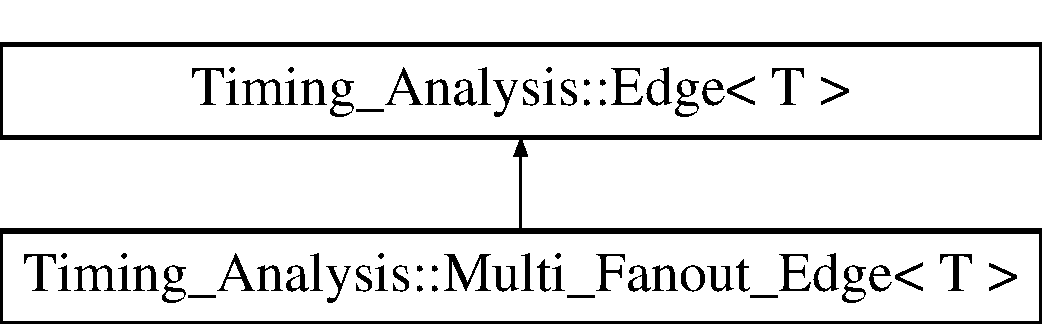
\includegraphics[height=2.000000cm]{classTiming__Analysis_1_1Multi__Fanout__Edge}
\end{center}
\end{figure}
\subsection*{Public Member Functions}
\begin{DoxyCompactItemize}
\item 
\hyperlink{classTiming__Analysis_1_1Multi__Fanout__Edge_a877f7672fb4fbabf49943fd3c86b7f59}{Multi\-\_\-\-Fanout\-\_\-\-Edge} (T $\ast$\hyperlink{classTiming__Analysis_1_1Edge_a47020ea89fd9fde438adc814a731a23d}{from})
\begin{DoxyCompactList}\small\item\em \hyperlink{classTiming__Analysis_1_1Multi__Fanout__Edge}{Multi\-\_\-\-Fanout\-\_\-\-Edge} constructor. \end{DoxyCompactList}\item 
T \& \hyperlink{classTiming__Analysis_1_1Multi__Fanout__Edge_a77ac79088e9ef11d222e777e2963f676}{to} (const int i) const 
\begin{DoxyCompactList}\small\item\em Returns Edge$<$\-T$>$ at index i. \end{DoxyCompactList}\end{DoxyCompactItemize}
\subsection*{Additional Inherited Members}


\subsection{Detailed Description}
\subsubsection*{template$<$class T$>$class Timing\-\_\-\-Analysis\-::\-Multi\-\_\-\-Fanout\-\_\-\-Edge$<$ T $>$}

Inherits from \hyperlink{classTiming__Analysis_1_1Edge}{Edge}. An multi fanout edge is a group of edges which connects a vertex to more than one vertexes. 



\subsection{Constructor \& Destructor Documentation}
\hypertarget{classTiming__Analysis_1_1Multi__Fanout__Edge_a877f7672fb4fbabf49943fd3c86b7f59}{\index{Timing\-\_\-\-Analysis\-::\-Multi\-\_\-\-Fanout\-\_\-\-Edge@{Timing\-\_\-\-Analysis\-::\-Multi\-\_\-\-Fanout\-\_\-\-Edge}!Multi\-\_\-\-Fanout\-\_\-\-Edge@{Multi\-\_\-\-Fanout\-\_\-\-Edge}}
\index{Multi\-\_\-\-Fanout\-\_\-\-Edge@{Multi\-\_\-\-Fanout\-\_\-\-Edge}!Timing_Analysis::Multi_Fanout_Edge@{Timing\-\_\-\-Analysis\-::\-Multi\-\_\-\-Fanout\-\_\-\-Edge}}
\subsubsection[{Multi\-\_\-\-Fanout\-\_\-\-Edge}]{\setlength{\rightskip}{0pt plus 5cm}template$<$class T$>$ {\bf Timing\-\_\-\-Analysis\-::\-Multi\-\_\-\-Fanout\-\_\-\-Edge}$<$ T $>$\-::{\bf Multi\-\_\-\-Fanout\-\_\-\-Edge} (
\begin{DoxyParamCaption}
\item[{T $\ast$}]{from}
\end{DoxyParamCaption}
)\hspace{0.3cm}{\ttfamily [inline]}}}\label{classTiming__Analysis_1_1Multi__Fanout__Edge_a877f7672fb4fbabf49943fd3c86b7f59}


\hyperlink{classTiming__Analysis_1_1Multi__Fanout__Edge}{Multi\-\_\-\-Fanout\-\_\-\-Edge} constructor. 



\subsection{Member Function Documentation}
\hypertarget{classTiming__Analysis_1_1Multi__Fanout__Edge_a77ac79088e9ef11d222e777e2963f676}{\index{Timing\-\_\-\-Analysis\-::\-Multi\-\_\-\-Fanout\-\_\-\-Edge@{Timing\-\_\-\-Analysis\-::\-Multi\-\_\-\-Fanout\-\_\-\-Edge}!to@{to}}
\index{to@{to}!Timing_Analysis::Multi_Fanout_Edge@{Timing\-\_\-\-Analysis\-::\-Multi\-\_\-\-Fanout\-\_\-\-Edge}}
\subsubsection[{to}]{\setlength{\rightskip}{0pt plus 5cm}template$<$class T$>$ T\& {\bf Timing\-\_\-\-Analysis\-::\-Multi\-\_\-\-Fanout\-\_\-\-Edge}$<$ T $>$\-::to (
\begin{DoxyParamCaption}
\item[{const int}]{i}
\end{DoxyParamCaption}
) const\hspace{0.3cm}{\ttfamily [inline]}}}\label{classTiming__Analysis_1_1Multi__Fanout__Edge_a77ac79088e9ef11d222e777e2963f676}


Returns Edge$<$\-T$>$ at index i. 


\begin{DoxyParams}{Parameters}
{\em const} & int i\\
\hline
\end{DoxyParams}
\begin{DoxyReturn}{Returns}
T \& 
\end{DoxyReturn}


The documentation for this class was generated from the following file\-:\begin{DoxyCompactItemize}
\item 
tcc\-Chrystian/src/include/multi\-\_\-fanout\-\_\-edge.\-h\end{DoxyCompactItemize}

\hypertarget{structCircuit__Netlist_1_1Net}{\section{Circuit\-\_\-\-Netlist\-:\-:Net Struct Reference}
\label{structCircuit__Netlist_1_1Net}\index{Circuit\-\_\-\-Netlist\-::\-Net@{Circuit\-\_\-\-Netlist\-::\-Net}}
}


Struct which represents a \hyperlink{structCircuit__Netlist_1_1Net}{Net}, which connect two or more circuit elements together.  




{\ttfamily \#include $<$circuit\-\_\-netlist.\-h$>$}

\subsection*{Public Member Functions}
\begin{DoxyCompactItemize}
\item 
\hyperlink{structCircuit__Netlist_1_1Net_acebd510f80cda6c9c480b5e313978895}{Net} (const string name, const int source\-Node, const string source\-Pin, const bool dummy\-Net=false)
\begin{DoxyCompactList}\small\item\em \hyperlink{structCircuit__Netlist_1_1Net}{Net} constructor. \end{DoxyCompactList}\item 
void \hyperlink{structCircuit__Netlist_1_1Net_af5bf832949516e3d7e16957206809027}{add\-Sink} (const \hyperlink{structCircuit__Netlist_1_1Sink}{Sink} sink\-Node)
\begin{DoxyCompactList}\small\item\em Adds sink to sinks list. \end{DoxyCompactList}\end{DoxyCompactItemize}
\subsection*{Public Attributes}
\begin{DoxyCompactItemize}
\item 
\hypertarget{structCircuit__Netlist_1_1Net_aaf85019638c09259b055dc0d1352054a}{string {\bfseries name}}\label{structCircuit__Netlist_1_1Net_aaf85019638c09259b055dc0d1352054a}

\item 
\hypertarget{structCircuit__Netlist_1_1Net_a92ee3950fbcbe247f1d98c180ebb4813}{int {\bfseries source\-Node}}\label{structCircuit__Netlist_1_1Net_a92ee3950fbcbe247f1d98c180ebb4813}

\item 
\hypertarget{structCircuit__Netlist_1_1Net_a44ebd7aa36b2d81b127527a09654f99e}{string {\bfseries source\-Pin}}\label{structCircuit__Netlist_1_1Net_a44ebd7aa36b2d81b127527a09654f99e}

\item 
\hypertarget{structCircuit__Netlist_1_1Net_a99d49ffd915347f780cae8fa9cbbd841}{vector$<$ \hyperlink{structCircuit__Netlist_1_1Sink}{Sink} $>$ {\bfseries sinks}}\label{structCircuit__Netlist_1_1Net_a99d49ffd915347f780cae8fa9cbbd841}

\item 
\hypertarget{structCircuit__Netlist_1_1Net_aad21a10a91330fd07d89ffccf21b55f8}{bool {\bfseries dummy\-Net}}\label{structCircuit__Netlist_1_1Net_aad21a10a91330fd07d89ffccf21b55f8}

\end{DoxyCompactItemize}


\subsection{Detailed Description}
Struct which represents a \hyperlink{structCircuit__Netlist_1_1Net}{Net}, which connect two or more circuit elements together. 



\subsection{Constructor \& Destructor Documentation}
\hypertarget{structCircuit__Netlist_1_1Net_acebd510f80cda6c9c480b5e313978895}{\index{Circuit\-\_\-\-Netlist\-::\-Net@{Circuit\-\_\-\-Netlist\-::\-Net}!Net@{Net}}
\index{Net@{Net}!Circuit_Netlist::Net@{Circuit\-\_\-\-Netlist\-::\-Net}}
\subsubsection[{Net}]{\setlength{\rightskip}{0pt plus 5cm}Circuit\-\_\-\-Netlist\-::\-Net\-::\-Net (
\begin{DoxyParamCaption}
\item[{const string}]{name, }
\item[{const int}]{source\-Node, }
\item[{const string}]{source\-Pin, }
\item[{const bool}]{dummy\-Net = {\ttfamily false}}
\end{DoxyParamCaption}
)\hspace{0.3cm}{\ttfamily [inline]}}}\label{structCircuit__Netlist_1_1Net_acebd510f80cda6c9c480b5e313978895}


\hyperlink{structCircuit__Netlist_1_1Net}{Net} constructor. 


\begin{DoxyParams}{Parameters}
{\em const} & string name, const int source\-Node, const string source\-Pin, const bool dummy\-Net(false default) \\
\hline
\end{DoxyParams}


\subsection{Member Function Documentation}
\hypertarget{structCircuit__Netlist_1_1Net_af5bf832949516e3d7e16957206809027}{\index{Circuit\-\_\-\-Netlist\-::\-Net@{Circuit\-\_\-\-Netlist\-::\-Net}!add\-Sink@{add\-Sink}}
\index{add\-Sink@{add\-Sink}!Circuit_Netlist::Net@{Circuit\-\_\-\-Netlist\-::\-Net}}
\subsubsection[{add\-Sink}]{\setlength{\rightskip}{0pt plus 5cm}void Circuit\-\_\-\-Netlist\-::\-Net\-::add\-Sink (
\begin{DoxyParamCaption}
\item[{const {\bf Sink}}]{sink\-Node}
\end{DoxyParamCaption}
)\hspace{0.3cm}{\ttfamily [inline]}}}\label{structCircuit__Netlist_1_1Net_af5bf832949516e3d7e16957206809027}


Adds sink to sinks list. 


\begin{DoxyParams}{Parameters}
{\em const} & \hyperlink{structCircuit__Netlist_1_1Sink}{Sink} sink\-Node\\
\hline
\end{DoxyParams}
\begin{DoxyReturn}{Returns}
void 
\end{DoxyReturn}


The documentation for this struct was generated from the following file\-:\begin{DoxyCompactItemize}
\item 
tcc\-Chrystian/src/include/circuit\-\_\-netlist.\-h\end{DoxyCompactItemize}

\hypertarget{structSpefNetISPD2013_1_1Node}{\section{Spef\-Net\-I\-S\-P\-D2013\-:\-:Node Struct Reference}
\label{structSpefNetISPD2013_1_1Node}\index{Spef\-Net\-I\-S\-P\-D2013\-::\-Node@{Spef\-Net\-I\-S\-P\-D2013\-::\-Node}}
}


Struct which represents a node of the circuit. A node is a point of the circuit where two or more elements meet.  




{\ttfamily \#include $<$spef\-\_\-net.\-h$>$}

\subsection*{Public Member Functions}
\begin{DoxyCompactItemize}
\item 
\hyperlink{structSpefNetISPD2013_1_1Node_afe9790ca4fcf757354ffb0dc3b578646}{Node} (const int \&index, const string \&name)
\begin{DoxyCompactList}\small\item\em \hyperlink{structSpefNetISPD2013_1_1Node}{Node} constructor. \end{DoxyCompactList}\end{DoxyCompactItemize}
\subsection*{Public Attributes}
\begin{DoxyCompactItemize}
\item 
\hypertarget{structSpefNetISPD2013_1_1Node_ae2b9605ff0872b8b12a8bc27e1a89540}{int {\bfseries node\-Index}}\label{structSpefNetISPD2013_1_1Node_ae2b9605ff0872b8b12a8bc27e1a89540}

\item 
\hypertarget{structSpefNetISPD2013_1_1Node_a7bc1303eeb250a3f7e047b8ec03d5e3e}{string {\bfseries name}}\label{structSpefNetISPD2013_1_1Node_a7bc1303eeb250a3f7e047b8ec03d5e3e}

\item 
\hypertarget{structSpefNetISPD2013_1_1Node_a0fe85a2441e7652f6a593abd9460ac85}{vector$<$ int $>$ {\bfseries resistors}}\label{structSpefNetISPD2013_1_1Node_a0fe85a2441e7652f6a593abd9460ac85}

\item 
\hypertarget{structSpefNetISPD2013_1_1Node_ae5a332384e934554beee8f743670506d}{double {\bfseries capacitance}}\label{structSpefNetISPD2013_1_1Node_ae5a332384e934554beee8f743670506d}

\end{DoxyCompactItemize}


\subsection{Detailed Description}
Struct which represents a node of the circuit. A node is a point of the circuit where two or more elements meet. 



\subsection{Constructor \& Destructor Documentation}
\hypertarget{structSpefNetISPD2013_1_1Node_afe9790ca4fcf757354ffb0dc3b578646}{\index{Spef\-Net\-I\-S\-P\-D2013\-::\-Node@{Spef\-Net\-I\-S\-P\-D2013\-::\-Node}!Node@{Node}}
\index{Node@{Node}!SpefNetISPD2013::Node@{Spef\-Net\-I\-S\-P\-D2013\-::\-Node}}
\subsubsection[{Node}]{\setlength{\rightskip}{0pt plus 5cm}Spef\-Net\-I\-S\-P\-D2013\-::\-Node\-::\-Node (
\begin{DoxyParamCaption}
\item[{const int \&}]{index, }
\item[{const string \&}]{name}
\end{DoxyParamCaption}
)\hspace{0.3cm}{\ttfamily [inline]}}}\label{structSpefNetISPD2013_1_1Node_afe9790ca4fcf757354ffb0dc3b578646}


\hyperlink{structSpefNetISPD2013_1_1Node}{Node} constructor. 


\begin{DoxyParams}{Parameters}
{\em const} & int \& index, const string \& name \\
\hline
\end{DoxyParams}


The documentation for this struct was generated from the following file\-:\begin{DoxyCompactItemize}
\item 
tcc\-Chrystian/src/include/spef\-\_\-net.\-h\end{DoxyCompactItemize}

\hypertarget{classstd_1_1numeric__limits_3_01Transitions_3_01double_01_4_01_4}{\section{std\-:\-:numeric\-\_\-limits$<$ Transitions$<$ double $>$ $>$ Class Template Reference}
\label{classstd_1_1numeric__limits_3_01Transitions_3_01double_01_4_01_4}\index{std\-::numeric\-\_\-limits$<$ Transitions$<$ double $>$ $>$@{std\-::numeric\-\_\-limits$<$ Transitions$<$ double $>$ $>$}}
}


Class used to make easier to work with double variable numeric limits.  




{\ttfamily \#include $<$transitions.\-h$>$}

\subsection*{Static Public Member Functions}
\begin{DoxyCompactItemize}
\item 
static \hyperlink{classTransitions}{Transitions}$<$ double $>$ \hyperlink{classstd_1_1numeric__limits_3_01Transitions_3_01double_01_4_01_4_aaf2bf171cb5f11b864b09798f6d63460}{min} ()
\begin{DoxyCompactList}\small\item\em Sets Returns a Transition with the minimum values of rise and fall times possible in I\-E\-E\-E floating point double precision representation. \end{DoxyCompactList}\item 
static \hyperlink{classTransitions}{Transitions}$<$ double $>$ \hyperlink{classstd_1_1numeric__limits_3_01Transitions_3_01double_01_4_01_4_aac0b30f8990c636cda3f083b95e626a4}{max} ()
\begin{DoxyCompactList}\small\item\em Sets Returns a Transition with the maximum values of rise and fall times possible in I\-E\-E\-E floating point double precision representation. \end{DoxyCompactList}\item 
static \hyperlink{classTransitions}{Transitions}$<$ double $>$ \hyperlink{classstd_1_1numeric__limits_3_01Transitions_3_01double_01_4_01_4_ab17fbee311d6e67204ca678d02ba1e80}{zero} ()
\begin{DoxyCompactList}\small\item\em Sets Returns a Transition with value zero for rise and fall times. \end{DoxyCompactList}\end{DoxyCompactItemize}


\subsection{Detailed Description}
\subsubsection*{template$<$$>$class std\-::numeric\-\_\-limits$<$ Transitions$<$ double $>$ $>$}

Class used to make easier to work with double variable numeric limits. 



\subsection{Member Function Documentation}
\hypertarget{classstd_1_1numeric__limits_3_01Transitions_3_01double_01_4_01_4_aac0b30f8990c636cda3f083b95e626a4}{\index{std\-::numeric\-\_\-limits$<$ Transitions$<$ double $>$ $>$@{std\-::numeric\-\_\-limits$<$ Transitions$<$ double $>$ $>$}!max@{max}}
\index{max@{max}!std::numeric_limits< Transitions< double > >@{std\-::numeric\-\_\-limits$<$ Transitions$<$ double $>$ $>$}}
\subsubsection[{max}]{\setlength{\rightskip}{0pt plus 5cm}static {\bf Transitions}$<$double$>$ std\-::numeric\-\_\-limits$<$ {\bf Transitions}$<$ double $>$ $>$\-::max (
\begin{DoxyParamCaption}
{}
\end{DoxyParamCaption}
)\hspace{0.3cm}{\ttfamily [inline]}, {\ttfamily [static]}}}\label{classstd_1_1numeric__limits_3_01Transitions_3_01double_01_4_01_4_aac0b30f8990c636cda3f083b95e626a4}


Sets Returns a Transition with the maximum values of rise and fall times possible in I\-E\-E\-E floating point double precision representation. 

\begin{DoxyReturn}{Returns}
\hyperlink{classTransitions}{Transitions$<$double$>$} 
\end{DoxyReturn}
\hypertarget{classstd_1_1numeric__limits_3_01Transitions_3_01double_01_4_01_4_aaf2bf171cb5f11b864b09798f6d63460}{\index{std\-::numeric\-\_\-limits$<$ Transitions$<$ double $>$ $>$@{std\-::numeric\-\_\-limits$<$ Transitions$<$ double $>$ $>$}!min@{min}}
\index{min@{min}!std::numeric_limits< Transitions< double > >@{std\-::numeric\-\_\-limits$<$ Transitions$<$ double $>$ $>$}}
\subsubsection[{min}]{\setlength{\rightskip}{0pt plus 5cm}static {\bf Transitions}$<$double$>$ std\-::numeric\-\_\-limits$<$ {\bf Transitions}$<$ double $>$ $>$\-::min (
\begin{DoxyParamCaption}
{}
\end{DoxyParamCaption}
)\hspace{0.3cm}{\ttfamily [inline]}, {\ttfamily [static]}}}\label{classstd_1_1numeric__limits_3_01Transitions_3_01double_01_4_01_4_aaf2bf171cb5f11b864b09798f6d63460}


Sets Returns a Transition with the minimum values of rise and fall times possible in I\-E\-E\-E floating point double precision representation. 

\begin{DoxyReturn}{Returns}
\hyperlink{classTransitions}{Transitions$<$double$>$} 
\end{DoxyReturn}
\hypertarget{classstd_1_1numeric__limits_3_01Transitions_3_01double_01_4_01_4_ab17fbee311d6e67204ca678d02ba1e80}{\index{std\-::numeric\-\_\-limits$<$ Transitions$<$ double $>$ $>$@{std\-::numeric\-\_\-limits$<$ Transitions$<$ double $>$ $>$}!zero@{zero}}
\index{zero@{zero}!std::numeric_limits< Transitions< double > >@{std\-::numeric\-\_\-limits$<$ Transitions$<$ double $>$ $>$}}
\subsubsection[{zero}]{\setlength{\rightskip}{0pt plus 5cm}static {\bf Transitions}$<$double$>$ std\-::numeric\-\_\-limits$<$ {\bf Transitions}$<$ double $>$ $>$\-::zero (
\begin{DoxyParamCaption}
{}
\end{DoxyParamCaption}
)\hspace{0.3cm}{\ttfamily [inline]}, {\ttfamily [static]}}}\label{classstd_1_1numeric__limits_3_01Transitions_3_01double_01_4_01_4_ab17fbee311d6e67204ca678d02ba1e80}


Sets Returns a Transition with value zero for rise and fall times. 

\begin{DoxyReturn}{Returns}
\hyperlink{classTransitions}{Transitions$<$double$>$} 
\end{DoxyReturn}


The documentation for this class was generated from the following file\-:\begin{DoxyCompactItemize}
\item 
tcc\-Chrystian/src/include/transitions.\-h\end{DoxyCompactItemize}

\hypertarget{classTiming__Analysis_1_1Option}{\section{Timing\-\_\-\-Analysis\-:\-:Option Class Reference}
\label{classTiming__Analysis_1_1Option}\index{Timing\-\_\-\-Analysis\-::\-Option@{Timing\-\_\-\-Analysis\-::\-Option}}
}


Refers to the implementation option of a logic gate.  




{\ttfamily \#include $<$timing\-\_\-analysis.\-h$>$}



Collaboration diagram for Timing\-\_\-\-Analysis\-:\-:Option\-:\nopagebreak
\begin{figure}[H]
\begin{center}
\leavevmode
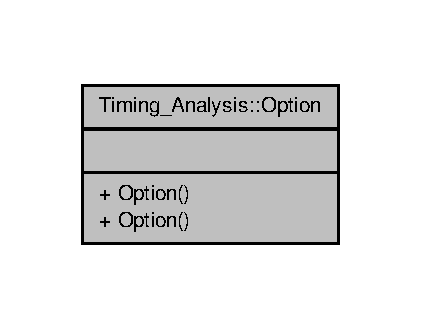
\includegraphics[width=202pt]{classTiming__Analysis_1_1Option__coll__graph}
\end{center}
\end{figure}
\subsection*{Public Member Functions}
\begin{DoxyCompactItemize}
\item 
\hyperlink{classTiming__Analysis_1_1Option_ac426169d74c9d432f168255b6cb52544}{Option} ()
\begin{DoxyCompactList}\small\item\em \hyperlink{classTiming__Analysis_1_1Option}{Option} default constructor. \end{DoxyCompactList}\item 
\hyperlink{classTiming__Analysis_1_1Option_a1d95559d49ea714e293a8679cefe8295}{Option} (const int footprint\-Index, const int option\-Index)
\begin{DoxyCompactList}\small\item\em \hyperlink{classTiming__Analysis_1_1Option}{Option} default constructor. \end{DoxyCompactList}\end{DoxyCompactItemize}
\subsection*{Friends}
\begin{DoxyCompactItemize}
\item 
class \hyperlink{classTiming__Analysis_1_1Option_aab560f9cdcd55852a6a08a29a54a2b16}{Timing\-\_\-\-Analysis}
\end{DoxyCompactItemize}


\subsection{Detailed Description}
Refers to the implementation option of a logic gate. 

\subsection{Constructor \& Destructor Documentation}
\hypertarget{classTiming__Analysis_1_1Option_ac426169d74c9d432f168255b6cb52544}{\index{Timing\-\_\-\-Analysis\-::\-Option@{Timing\-\_\-\-Analysis\-::\-Option}!Option@{Option}}
\index{Option@{Option}!Timing_Analysis::Option@{Timing\-\_\-\-Analysis\-::\-Option}}
\subsubsection[{Option}]{\setlength{\rightskip}{0pt plus 5cm}Timing\-\_\-\-Analysis\-::\-Option\-::\-Option (
\begin{DoxyParamCaption}
{}
\end{DoxyParamCaption}
)\hspace{0.3cm}{\ttfamily [inline]}}}\label{classTiming__Analysis_1_1Option_ac426169d74c9d432f168255b6cb52544}


\hyperlink{classTiming__Analysis_1_1Option}{Option} default constructor. 

\hypertarget{classTiming__Analysis_1_1Option_a1d95559d49ea714e293a8679cefe8295}{\index{Timing\-\_\-\-Analysis\-::\-Option@{Timing\-\_\-\-Analysis\-::\-Option}!Option@{Option}}
\index{Option@{Option}!Timing_Analysis::Option@{Timing\-\_\-\-Analysis\-::\-Option}}
\subsubsection[{Option}]{\setlength{\rightskip}{0pt plus 5cm}Timing\-\_\-\-Analysis\-::\-Option\-::\-Option (
\begin{DoxyParamCaption}
\item[{const int}]{footprint\-Index, }
\item[{const int}]{option\-Index}
\end{DoxyParamCaption}
)\hspace{0.3cm}{\ttfamily [inline]}}}\label{classTiming__Analysis_1_1Option_a1d95559d49ea714e293a8679cefe8295}


\hyperlink{classTiming__Analysis_1_1Option}{Option} default constructor. 


\begin{DoxyParams}{Parameters}
{\em const} & int footprint\-Index, const int option\-Index \\
\hline
\end{DoxyParams}


\subsection{Friends And Related Function Documentation}
\hypertarget{classTiming__Analysis_1_1Option_aab560f9cdcd55852a6a08a29a54a2b16}{\index{Timing\-\_\-\-Analysis\-::\-Option@{Timing\-\_\-\-Analysis\-::\-Option}!Timing\-\_\-\-Analysis@{Timing\-\_\-\-Analysis}}
\index{Timing\-\_\-\-Analysis@{Timing\-\_\-\-Analysis}!Timing_Analysis::Option@{Timing\-\_\-\-Analysis\-::\-Option}}
\subsubsection[{Timing\-\_\-\-Analysis}]{\setlength{\rightskip}{0pt plus 5cm}friend class {\bf Timing\-\_\-\-Analysis}\hspace{0.3cm}{\ttfamily [friend]}}}\label{classTiming__Analysis_1_1Option_aab560f9cdcd55852a6a08a29a54a2b16}


The documentation for this class was generated from the following file\-:\begin{DoxyCompactItemize}
\item 
Timing\-Analysis/src/include/\hyperlink{timing__analysis_8h}{timing\-\_\-analysis.\-h}\end{DoxyCompactItemize}

\hypertarget{classParser}{\section{Parser Class Reference}
\label{classParser}\index{Parser@{Parser}}
}
Inheritance diagram for Parser\-:\begin{figure}[H]
\begin{center}
\leavevmode
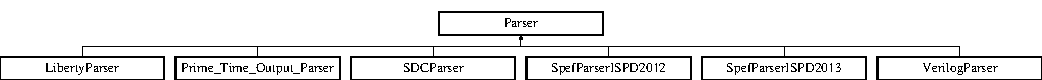
\includegraphics[height=1.072797cm]{classParser}
\end{center}
\end{figure}
\subsection*{Public Member Functions}
\begin{DoxyCompactItemize}
\item 
\hypertarget{classParser_a12234f6cd36b61af4b50c94a179422c1}{\hyperlink{classParser_a12234f6cd36b61af4b50c94a179422c1}{Parser} ()}\label{classParser_a12234f6cd36b61af4b50c94a179422c1}

\begin{DoxyCompactList}\small\item\em Empty \hyperlink{classParser}{Parser} constructor. \end{DoxyCompactList}\item 
\hypertarget{classParser_ad576b92b9cc324f6f41b0269a9a1a546}{virtual \hyperlink{classParser_ad576b92b9cc324f6f41b0269a9a1a546}{$\sim$\-Parser} ()}\label{classParser_ad576b92b9cc324f6f41b0269a9a1a546}

\begin{DoxyCompactList}\small\item\em Empty \hyperlink{classParser}{Parser} destructor. \end{DoxyCompactList}\end{DoxyCompactItemize}
\subsection*{Protected Member Functions}
\begin{DoxyCompactItemize}
\item 
\hypertarget{classParser_a83c7ac58f2c98cc54e9c750b29e6b0f0}{bool {\bfseries is\-Special\-Char} (const char \&c)}\label{classParser_a83c7ac58f2c98cc54e9c750b29e6b0f0}

\item 
\hypertarget{classParser_ae42067f51acd49ccccb0b0373321a421}{bool {\bfseries read\-Line\-As\-Tokens} (istream \&is, vector$<$ string $>$ \&tokens, bool include\-Special\-Chars=false)}\label{classParser_ae42067f51acd49ccccb0b0373321a421}

\end{DoxyCompactItemize}
\subsection*{Protected Attributes}
\begin{DoxyCompactItemize}
\item 
\hypertarget{classParser_a74c323dd4798b459fa982295b8e871bc}{fstream {\bfseries is}}\label{classParser_a74c323dd4798b459fa982295b8e871bc}

\end{DoxyCompactItemize}


The documentation for this class was generated from the following file\-:\begin{DoxyCompactItemize}
\item 
tcc\-Chrystian/src/include/parser.\-h\end{DoxyCompactItemize}

\hypertarget{structPrime__Time__Output__Parser_1_1Pin__Timing}{\section{Prime\-\_\-\-Time\-\_\-\-Output\-\_\-\-Parser\-:\-:Pin\-\_\-\-Timing Struct Reference}
\label{structPrime__Time__Output__Parser_1_1Pin__Timing}\index{Prime\-\_\-\-Time\-\_\-\-Output\-\_\-\-Parser\-::\-Pin\-\_\-\-Timing@{Prime\-\_\-\-Time\-\_\-\-Output\-\_\-\-Parser\-::\-Pin\-\_\-\-Timing}}
}


Struct containing the timing values of a pin.  




{\ttfamily \#include $<$parser.\-h$>$}

\subsection*{Public Attributes}
\begin{DoxyCompactItemize}
\item 
\hypertarget{structPrime__Time__Output__Parser_1_1Pin__Timing_adf3b868ae9f5a9cf5fa4605431bef741}{string {\bfseries pin\-\_\-name}}\label{structPrime__Time__Output__Parser_1_1Pin__Timing_adf3b868ae9f5a9cf5fa4605431bef741}

\item 
\hypertarget{structPrime__Time__Output__Parser_1_1Pin__Timing_a9619e81ea7b859c6c600daaaf3754051}{\hyperlink{classTransitions}{Transitions}$<$ double $>$ {\bfseries slack}}\label{structPrime__Time__Output__Parser_1_1Pin__Timing_a9619e81ea7b859c6c600daaaf3754051}

\item 
\hypertarget{structPrime__Time__Output__Parser_1_1Pin__Timing_af7d7bae7417f6586e445c5bb415a1d43}{\hyperlink{classTransitions}{Transitions}$<$ double $>$ {\bfseries slew}}\label{structPrime__Time__Output__Parser_1_1Pin__Timing_af7d7bae7417f6586e445c5bb415a1d43}

\item 
\hypertarget{structPrime__Time__Output__Parser_1_1Pin__Timing_a2737c385dec9bd775aa20f860293fbd0}{\hyperlink{classTransitions}{Transitions}$<$ double $>$ {\bfseries arrival\-\_\-time}}\label{structPrime__Time__Output__Parser_1_1Pin__Timing_a2737c385dec9bd775aa20f860293fbd0}

\end{DoxyCompactItemize}
\subsection*{Friends}
\begin{DoxyCompactItemize}
\item 
\hypertarget{structPrime__Time__Output__Parser_1_1Pin__Timing_a8ea07e765281219a4b6c4adf6c2274ea}{ostream \& \hyperlink{structPrime__Time__Output__Parser_1_1Pin__Timing_a8ea07e765281219a4b6c4adf6c2274ea}{operator$<$$<$} (ostream \&out, const \hyperlink{structPrime__Time__Output__Parser_1_1Pin__Timing}{Pin\-\_\-\-Timing} \&pin)}\label{structPrime__Time__Output__Parser_1_1Pin__Timing_a8ea07e765281219a4b6c4adf6c2274ea}

\begin{DoxyCompactList}\small\item\em Redefinition of $<$$<$ operator. Inserts formatted description including pin name and slack, slew and arrival time values. \end{DoxyCompactList}\end{DoxyCompactItemize}


\subsection{Detailed Description}
Struct containing the timing values of a pin. 

The documentation for this struct was generated from the following file\-:\begin{DoxyCompactItemize}
\item 
tcc\-Chrystian/src/include/parser.\-h\end{DoxyCompactItemize}

\hypertarget{structPrime__Time__Output__Parser_1_1Port__Timing}{\section{Prime\-\_\-\-Time\-\_\-\-Output\-\_\-\-Parser\-:\-:Port\-\_\-\-Timing Struct Reference}
\label{structPrime__Time__Output__Parser_1_1Port__Timing}\index{Prime\-\_\-\-Time\-\_\-\-Output\-\_\-\-Parser\-::\-Port\-\_\-\-Timing@{Prime\-\_\-\-Time\-\_\-\-Output\-\_\-\-Parser\-::\-Port\-\_\-\-Timing}}
}


Struct containing the timing values of a port.  




{\ttfamily \#include $<$parser.\-h$>$}

\subsection*{Public Attributes}
\begin{DoxyCompactItemize}
\item 
\hypertarget{structPrime__Time__Output__Parser_1_1Port__Timing_a4c7ae6cb0e76db94fe3b03822ead72c4}{string {\bfseries port\-\_\-name}}\label{structPrime__Time__Output__Parser_1_1Port__Timing_a4c7ae6cb0e76db94fe3b03822ead72c4}

\item 
\hypertarget{structPrime__Time__Output__Parser_1_1Port__Timing_a21231dfc490477789c81e0c9e3e8c18d}{\hyperlink{classTransitions}{Transitions}$<$ double $>$ {\bfseries slack}}\label{structPrime__Time__Output__Parser_1_1Port__Timing_a21231dfc490477789c81e0c9e3e8c18d}

\item 
\hypertarget{structPrime__Time__Output__Parser_1_1Port__Timing_a33e7eb34b63367e3b639999e1cb793bf}{\hyperlink{classTransitions}{Transitions}$<$ double $>$ {\bfseries slew}}\label{structPrime__Time__Output__Parser_1_1Port__Timing_a33e7eb34b63367e3b639999e1cb793bf}

\end{DoxyCompactItemize}
\subsection*{Friends}
\begin{DoxyCompactItemize}
\item 
\hypertarget{structPrime__Time__Output__Parser_1_1Port__Timing_abd555e7dc2c5bfe2b1699915d6b0ca8f}{ostream \& \hyperlink{structPrime__Time__Output__Parser_1_1Port__Timing_abd555e7dc2c5bfe2b1699915d6b0ca8f}{operator$<$$<$} (ostream \&out, const \hyperlink{structPrime__Time__Output__Parser_1_1Port__Timing}{Port\-\_\-\-Timing} \&port)}\label{structPrime__Time__Output__Parser_1_1Port__Timing_abd555e7dc2c5bfe2b1699915d6b0ca8f}

\begin{DoxyCompactList}\small\item\em Redefinition of $<$$<$ operator. Inserts formatted description including port name, slack and slew time values. \end{DoxyCompactList}\end{DoxyCompactItemize}


\subsection{Detailed Description}
Struct containing the timing values of a port. 

The documentation for this struct was generated from the following file\-:\begin{DoxyCompactItemize}
\item 
tcc\-Chrystian/src/include/parser.\-h\end{DoxyCompactItemize}

\hypertarget{classPrime__Time__Output__Parser_1_1Prime__Time__Output}{\section{Prime\-\_\-\-Time\-\_\-\-Output\-\_\-\-Parser\-:\-:Prime\-\_\-\-Time\-\_\-\-Output Class Reference}
\label{classPrime__Time__Output__Parser_1_1Prime__Time__Output}\index{Prime\-\_\-\-Time\-\_\-\-Output\-\_\-\-Parser\-::\-Prime\-\_\-\-Time\-\_\-\-Output@{Prime\-\_\-\-Time\-\_\-\-Output\-\_\-\-Parser\-::\-Prime\-\_\-\-Time\-\_\-\-Output}}
}


Represents Prime Time output. Provides access methods to it.  




{\ttfamily \#include $<$parser.\-h$>$}



Collaboration diagram for Prime\-\_\-\-Time\-\_\-\-Output\-\_\-\-Parser\-:\-:Prime\-\_\-\-Time\-\_\-\-Output\-:\nopagebreak
\begin{figure}[H]
\begin{center}
\leavevmode
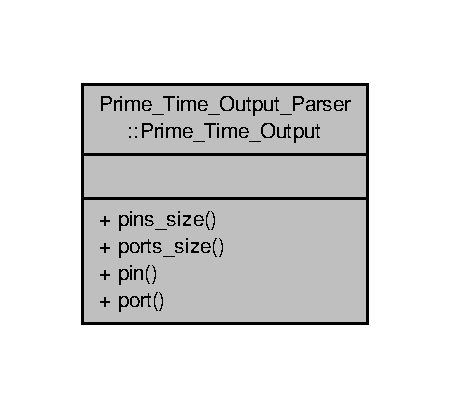
\includegraphics[width=216pt]{classPrime__Time__Output__Parser_1_1Prime__Time__Output__coll__graph}
\end{center}
\end{figure}
\subsection*{Public Member Functions}
\begin{DoxyCompactItemize}
\item 
size\-\_\-t \hyperlink{classPrime__Time__Output__Parser_1_1Prime__Time__Output_af89e7f909821e56d0e89ae62cebc5b81}{pins\-\_\-size} () const 
\begin{DoxyCompactList}\small\item\em Returns number of pins. \end{DoxyCompactList}\item 
size\-\_\-t \hyperlink{classPrime__Time__Output__Parser_1_1Prime__Time__Output_a6fdf8bbe0ea6ecdcdecec62e0922625f}{ports\-\_\-size} () const 
\begin{DoxyCompactList}\small\item\em Returns number of ports. \end{DoxyCompactList}\item 
const \hyperlink{structPrime__Time__Output__Parser_1_1Pin__Timing}{Pin\-\_\-\-Timing} \& \hyperlink{classPrime__Time__Output__Parser_1_1Prime__Time__Output_adfa3dff9af20ebb0872d4c775b3eeecc}{pin} (const size\-\_\-t i) const 
\begin{DoxyCompactList}\small\item\em Returns \hyperlink{structPrime__Time__Output__Parser_1_1Pin__Timing}{Pin\-\_\-\-Timing} reference at index i. \end{DoxyCompactList}\item 
const \hyperlink{structPrime__Time__Output__Parser_1_1Port__Timing}{Port\-\_\-\-Timing} \& \hyperlink{classPrime__Time__Output__Parser_1_1Prime__Time__Output_a36d4fa1cf4175cce9bac2fb27ea98f72}{port} (const size\-\_\-t i) const 
\begin{DoxyCompactList}\small\item\em Returns \hyperlink{structPrime__Time__Output__Parser_1_1Pin__Timing}{Pin\-\_\-\-Timing} reference at index i. \end{DoxyCompactList}\end{DoxyCompactItemize}
\subsection*{Friends}
\begin{DoxyCompactItemize}
\item 
class \hyperlink{classPrime__Time__Output__Parser_1_1Prime__Time__Output_add497bc1a470cf507522a48873d2b9b7}{Prime\-\_\-\-Time\-\_\-\-Output\-\_\-\-Parser}
\end{DoxyCompactItemize}


\subsection{Detailed Description}
Represents Prime Time output. Provides access methods to it. 

\subsection{Member Function Documentation}
\hypertarget{classPrime__Time__Output__Parser_1_1Prime__Time__Output_adfa3dff9af20ebb0872d4c775b3eeecc}{\index{Prime\-\_\-\-Time\-\_\-\-Output\-\_\-\-Parser\-::\-Prime\-\_\-\-Time\-\_\-\-Output@{Prime\-\_\-\-Time\-\_\-\-Output\-\_\-\-Parser\-::\-Prime\-\_\-\-Time\-\_\-\-Output}!pin@{pin}}
\index{pin@{pin}!Prime_Time_Output_Parser::Prime_Time_Output@{Prime\-\_\-\-Time\-\_\-\-Output\-\_\-\-Parser\-::\-Prime\-\_\-\-Time\-\_\-\-Output}}
\subsubsection[{pin}]{\setlength{\rightskip}{0pt plus 5cm}const {\bf Pin\-\_\-\-Timing}\& Prime\-\_\-\-Time\-\_\-\-Output\-\_\-\-Parser\-::\-Prime\-\_\-\-Time\-\_\-\-Output\-::pin (
\begin{DoxyParamCaption}
\item[{const size\-\_\-t}]{i}
\end{DoxyParamCaption}
) const\hspace{0.3cm}{\ttfamily [inline]}}}\label{classPrime__Time__Output__Parser_1_1Prime__Time__Output_adfa3dff9af20ebb0872d4c775b3eeecc}


Returns \hyperlink{structPrime__Time__Output__Parser_1_1Pin__Timing}{Pin\-\_\-\-Timing} reference at index i. 


\begin{DoxyParams}{Parameters}
{\em const} & size\-\_\-t i\\
\hline
\end{DoxyParams}
\begin{DoxyReturn}{Returns}
\hyperlink{structPrime__Time__Output__Parser_1_1Pin__Timing}{Pin\-\_\-\-Timing} \& 
\end{DoxyReturn}
\hypertarget{classPrime__Time__Output__Parser_1_1Prime__Time__Output_af89e7f909821e56d0e89ae62cebc5b81}{\index{Prime\-\_\-\-Time\-\_\-\-Output\-\_\-\-Parser\-::\-Prime\-\_\-\-Time\-\_\-\-Output@{Prime\-\_\-\-Time\-\_\-\-Output\-\_\-\-Parser\-::\-Prime\-\_\-\-Time\-\_\-\-Output}!pins\-\_\-size@{pins\-\_\-size}}
\index{pins\-\_\-size@{pins\-\_\-size}!Prime_Time_Output_Parser::Prime_Time_Output@{Prime\-\_\-\-Time\-\_\-\-Output\-\_\-\-Parser\-::\-Prime\-\_\-\-Time\-\_\-\-Output}}
\subsubsection[{pins\-\_\-size}]{\setlength{\rightskip}{0pt plus 5cm}size\-\_\-t Prime\-\_\-\-Time\-\_\-\-Output\-\_\-\-Parser\-::\-Prime\-\_\-\-Time\-\_\-\-Output\-::pins\-\_\-size (
\begin{DoxyParamCaption}
{}
\end{DoxyParamCaption}
) const\hspace{0.3cm}{\ttfamily [inline]}}}\label{classPrime__Time__Output__Parser_1_1Prime__Time__Output_af89e7f909821e56d0e89ae62cebc5b81}


Returns number of pins. 

\begin{DoxyReturn}{Returns}
size\-\_\-t 
\end{DoxyReturn}
\hypertarget{classPrime__Time__Output__Parser_1_1Prime__Time__Output_a36d4fa1cf4175cce9bac2fb27ea98f72}{\index{Prime\-\_\-\-Time\-\_\-\-Output\-\_\-\-Parser\-::\-Prime\-\_\-\-Time\-\_\-\-Output@{Prime\-\_\-\-Time\-\_\-\-Output\-\_\-\-Parser\-::\-Prime\-\_\-\-Time\-\_\-\-Output}!port@{port}}
\index{port@{port}!Prime_Time_Output_Parser::Prime_Time_Output@{Prime\-\_\-\-Time\-\_\-\-Output\-\_\-\-Parser\-::\-Prime\-\_\-\-Time\-\_\-\-Output}}
\subsubsection[{port}]{\setlength{\rightskip}{0pt plus 5cm}const {\bf Port\-\_\-\-Timing}\& Prime\-\_\-\-Time\-\_\-\-Output\-\_\-\-Parser\-::\-Prime\-\_\-\-Time\-\_\-\-Output\-::port (
\begin{DoxyParamCaption}
\item[{const size\-\_\-t}]{i}
\end{DoxyParamCaption}
) const\hspace{0.3cm}{\ttfamily [inline]}}}\label{classPrime__Time__Output__Parser_1_1Prime__Time__Output_a36d4fa1cf4175cce9bac2fb27ea98f72}


Returns \hyperlink{structPrime__Time__Output__Parser_1_1Pin__Timing}{Pin\-\_\-\-Timing} reference at index i. 


\begin{DoxyParams}{Parameters}
{\em const} & size\-\_\-t i\\
\hline
\end{DoxyParams}
\begin{DoxyReturn}{Returns}
\hyperlink{structPrime__Time__Output__Parser_1_1Port__Timing}{Port\-\_\-\-Timing} \& 
\end{DoxyReturn}
\hypertarget{classPrime__Time__Output__Parser_1_1Prime__Time__Output_a6fdf8bbe0ea6ecdcdecec62e0922625f}{\index{Prime\-\_\-\-Time\-\_\-\-Output\-\_\-\-Parser\-::\-Prime\-\_\-\-Time\-\_\-\-Output@{Prime\-\_\-\-Time\-\_\-\-Output\-\_\-\-Parser\-::\-Prime\-\_\-\-Time\-\_\-\-Output}!ports\-\_\-size@{ports\-\_\-size}}
\index{ports\-\_\-size@{ports\-\_\-size}!Prime_Time_Output_Parser::Prime_Time_Output@{Prime\-\_\-\-Time\-\_\-\-Output\-\_\-\-Parser\-::\-Prime\-\_\-\-Time\-\_\-\-Output}}
\subsubsection[{ports\-\_\-size}]{\setlength{\rightskip}{0pt plus 5cm}size\-\_\-t Prime\-\_\-\-Time\-\_\-\-Output\-\_\-\-Parser\-::\-Prime\-\_\-\-Time\-\_\-\-Output\-::ports\-\_\-size (
\begin{DoxyParamCaption}
{}
\end{DoxyParamCaption}
) const\hspace{0.3cm}{\ttfamily [inline]}}}\label{classPrime__Time__Output__Parser_1_1Prime__Time__Output_a6fdf8bbe0ea6ecdcdecec62e0922625f}


Returns number of ports. 

\begin{DoxyReturn}{Returns}
size\-\_\-t 
\end{DoxyReturn}


\subsection{Friends And Related Function Documentation}
\hypertarget{classPrime__Time__Output__Parser_1_1Prime__Time__Output_add497bc1a470cf507522a48873d2b9b7}{\index{Prime\-\_\-\-Time\-\_\-\-Output\-\_\-\-Parser\-::\-Prime\-\_\-\-Time\-\_\-\-Output@{Prime\-\_\-\-Time\-\_\-\-Output\-\_\-\-Parser\-::\-Prime\-\_\-\-Time\-\_\-\-Output}!Prime\-\_\-\-Time\-\_\-\-Output\-\_\-\-Parser@{Prime\-\_\-\-Time\-\_\-\-Output\-\_\-\-Parser}}
\index{Prime\-\_\-\-Time\-\_\-\-Output\-\_\-\-Parser@{Prime\-\_\-\-Time\-\_\-\-Output\-\_\-\-Parser}!Prime_Time_Output_Parser::Prime_Time_Output@{Prime\-\_\-\-Time\-\_\-\-Output\-\_\-\-Parser\-::\-Prime\-\_\-\-Time\-\_\-\-Output}}
\subsubsection[{Prime\-\_\-\-Time\-\_\-\-Output\-\_\-\-Parser}]{\setlength{\rightskip}{0pt plus 5cm}friend class {\bf Prime\-\_\-\-Time\-\_\-\-Output\-\_\-\-Parser}\hspace{0.3cm}{\ttfamily [friend]}}}\label{classPrime__Time__Output__Parser_1_1Prime__Time__Output_add497bc1a470cf507522a48873d2b9b7}


The documentation for this class was generated from the following file\-:\begin{DoxyCompactItemize}
\item 
Timing\-Analysis/src/include/\hyperlink{parser_8h}{parser.\-h}\end{DoxyCompactItemize}

\hypertarget{classPrime__Time__Output__Parser}{\section{Prime\-\_\-\-Time\-\_\-\-Output\-\_\-\-Parser Class Reference}
\label{classPrime__Time__Output__Parser}\index{Prime\-\_\-\-Time\-\_\-\-Output\-\_\-\-Parser@{Prime\-\_\-\-Time\-\_\-\-Output\-\_\-\-Parser}}
}


Inherits from \hyperlink{classParser}{Parser}. Parse the Prime Time output. Used to generate a \hyperlink{classPrime__Time__Output__Parser_1_1Prime__Time__Output}{Prime\-\_\-\-Time\-\_\-\-Output} object for later use.  




{\ttfamily \#include $<$parser.\-h$>$}

Inheritance diagram for Prime\-\_\-\-Time\-\_\-\-Output\-\_\-\-Parser\-:\begin{figure}[H]
\begin{center}
\leavevmode
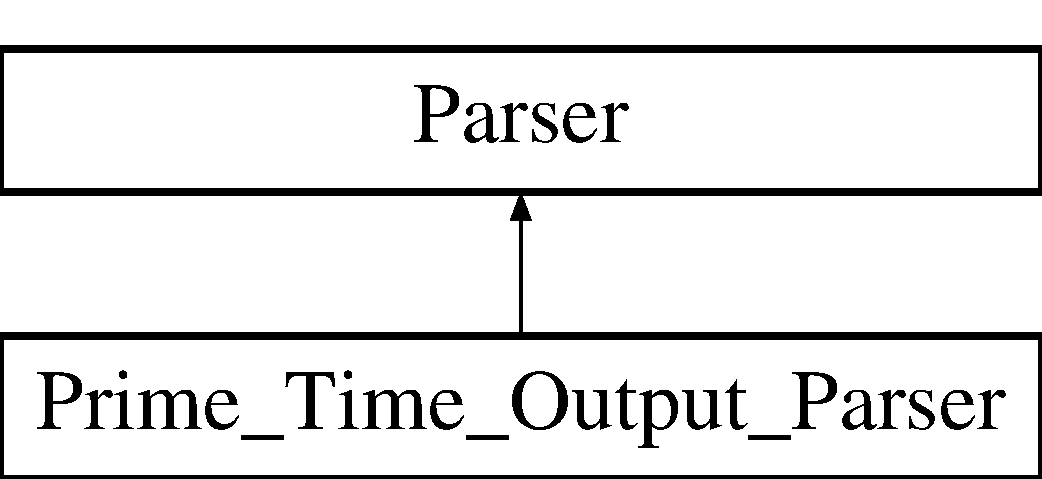
\includegraphics[height=2.000000cm]{classPrime__Time__Output__Parser}
\end{center}
\end{figure}
\subsection*{Classes}
\begin{DoxyCompactItemize}
\item 
struct \hyperlink{structPrime__Time__Output__Parser_1_1Pin__Timing}{Pin\-\_\-\-Timing}
\begin{DoxyCompactList}\small\item\em Struct containing the timing values of a pin. \end{DoxyCompactList}\item 
struct \hyperlink{structPrime__Time__Output__Parser_1_1Port__Timing}{Port\-\_\-\-Timing}
\begin{DoxyCompactList}\small\item\em Struct containing the timing values of a port. \end{DoxyCompactList}\item 
class \hyperlink{classPrime__Time__Output__Parser_1_1Prime__Time__Output}{Prime\-\_\-\-Time\-\_\-\-Output}
\begin{DoxyCompactList}\small\item\em Represents Prime Time output. Provides access methods to it. \end{DoxyCompactList}\end{DoxyCompactItemize}
\subsection*{Public Member Functions}
\begin{DoxyCompactItemize}
\item 
\hypertarget{classPrime__Time__Output__Parser_abbd1008efff182a6b8ce0f676b4ee823}{\hyperlink{classPrime__Time__Output__Parser_abbd1008efff182a6b8ce0f676b4ee823}{Prime\-\_\-\-Time\-\_\-\-Output\-\_\-\-Parser} ()}\label{classPrime__Time__Output__Parser_abbd1008efff182a6b8ce0f676b4ee823}

\begin{DoxyCompactList}\small\item\em \hyperlink{classPrime__Time__Output__Parser}{Prime\-\_\-\-Time\-\_\-\-Output\-\_\-\-Parser} empty constructor. \end{DoxyCompactList}\item 
const \hyperlink{classPrime__Time__Output__Parser_1_1Prime__Time__Output}{Prime\-\_\-\-Time\-\_\-\-Output} \hyperlink{classPrime__Time__Output__Parser_af43de199ba4575214a4d6e07fb980ca5}{parse\-\_\-prime\-\_\-time\-\_\-output\-\_\-file} (const string filename)
\begin{DoxyCompactList}\small\item\em Returns \hyperlink{classPrime__Time__Output__Parser_1_1Prime__Time__Output}{Prime\-\_\-\-Time\-\_\-\-Output} object generated using values read from file passed as filename parameter. \end{DoxyCompactList}\end{DoxyCompactItemize}
\subsection*{Additional Inherited Members}


\subsection{Detailed Description}
Inherits from \hyperlink{classParser}{Parser}. Parse the Prime Time output. Used to generate a \hyperlink{classPrime__Time__Output__Parser_1_1Prime__Time__Output}{Prime\-\_\-\-Time\-\_\-\-Output} object for later use. 

\subsection{Member Function Documentation}
\hypertarget{classPrime__Time__Output__Parser_af43de199ba4575214a4d6e07fb980ca5}{\index{Prime\-\_\-\-Time\-\_\-\-Output\-\_\-\-Parser@{Prime\-\_\-\-Time\-\_\-\-Output\-\_\-\-Parser}!parse\-\_\-prime\-\_\-time\-\_\-output\-\_\-file@{parse\-\_\-prime\-\_\-time\-\_\-output\-\_\-file}}
\index{parse\-\_\-prime\-\_\-time\-\_\-output\-\_\-file@{parse\-\_\-prime\-\_\-time\-\_\-output\-\_\-file}!Prime_Time_Output_Parser@{Prime\-\_\-\-Time\-\_\-\-Output\-\_\-\-Parser}}
\subsubsection[{parse\-\_\-prime\-\_\-time\-\_\-output\-\_\-file}]{\setlength{\rightskip}{0pt plus 5cm}const {\bf Prime\-\_\-\-Time\-\_\-\-Output} Prime\-\_\-\-Time\-\_\-\-Output\-\_\-\-Parser\-::parse\-\_\-prime\-\_\-time\-\_\-output\-\_\-file (
\begin{DoxyParamCaption}
\item[{const string}]{filename}
\end{DoxyParamCaption}
)}}\label{classPrime__Time__Output__Parser_af43de199ba4575214a4d6e07fb980ca5}


Returns \hyperlink{classPrime__Time__Output__Parser_1_1Prime__Time__Output}{Prime\-\_\-\-Time\-\_\-\-Output} object generated using values read from file passed as filename parameter. 


\begin{DoxyParams}{Parameters}
{\em const} & string filename\\
\hline
\end{DoxyParams}
\begin{DoxyReturn}{Returns}
const \hyperlink{classPrime__Time__Output__Parser_1_1Prime__Time__Output}{Prime\-\_\-\-Time\-\_\-\-Output} 
\end{DoxyReturn}


The documentation for this class was generated from the following file\-:\begin{DoxyCompactItemize}
\item 
tcc\-Chrystian/src/include/parser.\-h\end{DoxyCompactItemize}

\hypertarget{classRCTreeWireDelayModel}{\section{R\-C\-Tree\-Wire\-Delay\-Model Class Reference}
\label{classRCTreeWireDelayModel}\index{R\-C\-Tree\-Wire\-Delay\-Model@{R\-C\-Tree\-Wire\-Delay\-Model}}
}
Inheritance diagram for R\-C\-Tree\-Wire\-Delay\-Model\-:\begin{figure}[H]
\begin{center}
\leavevmode
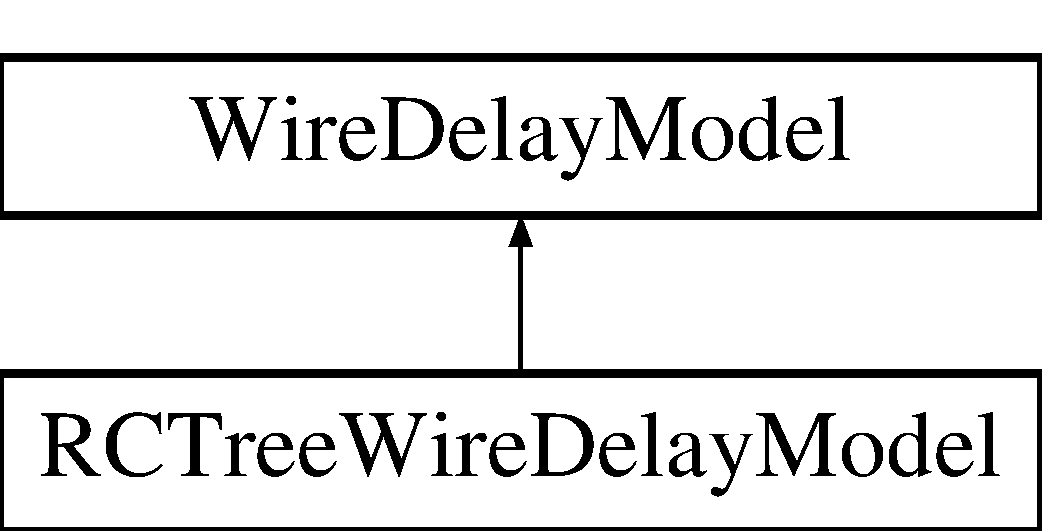
\includegraphics[height=2.000000cm]{classRCTreeWireDelayModel}
\end{center}
\end{figure}
\subsection*{Public Member Functions}
\begin{DoxyCompactItemize}
\item 
\hypertarget{classRCTreeWireDelayModel_a239d4784b2d39b6042fe39bee4838c6b}{{\bfseries R\-C\-Tree\-Wire\-Delay\-Model} (const \hyperlink{classSpefNetISPD2013}{Spef\-Net\-I\-S\-P\-D2013} \&descriptor, const string root\-Node, const size\-\_\-t arcs\-\_\-size, const bool dummy\-Edge=false)}\label{classRCTreeWireDelayModel_a239d4784b2d39b6042fe39bee4838c6b}

\item 
const \hyperlink{classTransitions}{Transitions}$<$ double $>$ \hyperlink{classRCTreeWireDelayModel_a06312bef3b98f0903335227fd7ea0f31}{simulate} (const \hyperlink{structLibertyCellInfo}{Liberty\-Cell\-Info} \&cell\-Info, const int input, const \hyperlink{classTransitions}{Transitions}$<$ double $>$ slew, bool is\-\_\-input\-\_\-driver)
\item 
const \hyperlink{classTransitions}{Transitions}$<$ double $>$ \hyperlink{classRCTreeWireDelayModel_a7c769d54e8a520db1c5d4537d7e8b608}{delay\-\_\-at\-\_\-fanout\-\_\-node} (const string fanout\-\_\-node\-\_\-name) const 
\begin{DoxyCompactList}\small\item\em Returns \hyperlink{classTransitions}{Transitions} with rise and fall delay time values set to zero. \end{DoxyCompactList}\item 
const \hyperlink{classTransitions}{Transitions}$<$ double $>$ \hyperlink{classRCTreeWireDelayModel_aea4c7315bdd3715ca0c67707b2c32a8c}{slew\-\_\-at\-\_\-fanout\-\_\-node} (const string fanout\-\_\-node\-\_\-name) const 
\begin{DoxyCompactList}\small\item\em Returns \hyperlink{classTransitions}{Transitions} with rise and fall slew time values set to zero. \end{DoxyCompactList}\item 
void \hyperlink{classRCTreeWireDelayModel_a106079b64e0e6b84327fc5a9b4c29a6a}{set\-Fanout\-Pin\-Capacitance} (const string fanout\-Name\-And\-Pin, const double pin\-Capacitance)
\begin{DoxyCompactList}\small\item\em Increments lumped capacitance of the wire. \end{DoxyCompactList}\item 
\hyperlink{classTransitions}{Transitions}$<$ double $>$ \hyperlink{classRCTreeWireDelayModel_a5575e4f4e598047dd87fee0707d135d3}{root\-\_\-delay} (int arc\-\_\-number)
\begin{DoxyCompactList}\small\item\em not yet implemented$\ast$$\ast$$\ast$$\ast$$\ast$$\ast$$\ast$$\ast$$\ast$$\ast$$\ast$$\ast$$\ast$$\ast$$\ast$$\ast$$\ast$$\ast$$\ast$$\ast$$\ast$$\ast$$\ast$ \end{DoxyCompactList}\item 
\hyperlink{classTransitions}{Transitions}$<$ double $>$ \hyperlink{classRCTreeWireDelayModel_aa314aa73bf2e25008d330ad19544e210}{root\-\_\-slew} (int arc\-\_\-number)
\begin{DoxyCompactList}\small\item\em not yet implemented$\ast$$\ast$$\ast$$\ast$$\ast$$\ast$$\ast$$\ast$$\ast$$\ast$$\ast$$\ast$$\ast$$\ast$$\ast$$\ast$$\ast$$\ast$$\ast$$\ast$$\ast$$\ast$$\ast$ \end{DoxyCompactList}\item 
void \hyperlink{classRCTreeWireDelayModel_acb14554ad26108d350770391b1923c51}{clear} ()
\begin{DoxyCompactList}\small\item\em not yet implemented$\ast$$\ast$$\ast$$\ast$$\ast$$\ast$$\ast$$\ast$$\ast$$\ast$$\ast$$\ast$$\ast$$\ast$$\ast$$\ast$$\ast$$\ast$$\ast$$\ast$$\ast$$\ast$ \end{DoxyCompactList}\end{DoxyCompactItemize}
\subsection*{Additional Inherited Members}


\subsection{Member Function Documentation}
\hypertarget{classRCTreeWireDelayModel_acb14554ad26108d350770391b1923c51}{\index{R\-C\-Tree\-Wire\-Delay\-Model@{R\-C\-Tree\-Wire\-Delay\-Model}!clear@{clear}}
\index{clear@{clear}!RCTreeWireDelayModel@{R\-C\-Tree\-Wire\-Delay\-Model}}
\subsubsection[{clear}]{\setlength{\rightskip}{0pt plus 5cm}void R\-C\-Tree\-Wire\-Delay\-Model\-::clear (
\begin{DoxyParamCaption}
{}
\end{DoxyParamCaption}
)\hspace{0.3cm}{\ttfamily [virtual]}}}\label{classRCTreeWireDelayModel_acb14554ad26108d350770391b1923c51}


not yet implemented$\ast$$\ast$$\ast$$\ast$$\ast$$\ast$$\ast$$\ast$$\ast$$\ast$$\ast$$\ast$$\ast$$\ast$$\ast$$\ast$$\ast$$\ast$$\ast$$\ast$$\ast$$\ast$ 

\begin{DoxyReturn}{Returns}
void 
\end{DoxyReturn}


Implements \hyperlink{classWireDelayModel_a74869a3a66deb53507e8bc6f16eff45c}{Wire\-Delay\-Model}.

\hypertarget{classRCTreeWireDelayModel_a7c769d54e8a520db1c5d4537d7e8b608}{\index{R\-C\-Tree\-Wire\-Delay\-Model@{R\-C\-Tree\-Wire\-Delay\-Model}!delay\-\_\-at\-\_\-fanout\-\_\-node@{delay\-\_\-at\-\_\-fanout\-\_\-node}}
\index{delay\-\_\-at\-\_\-fanout\-\_\-node@{delay\-\_\-at\-\_\-fanout\-\_\-node}!RCTreeWireDelayModel@{R\-C\-Tree\-Wire\-Delay\-Model}}
\subsubsection[{delay\-\_\-at\-\_\-fanout\-\_\-node}]{\setlength{\rightskip}{0pt plus 5cm}const {\bf Transitions}$<$double$>$ R\-C\-Tree\-Wire\-Delay\-Model\-::delay\-\_\-at\-\_\-fanout\-\_\-node (
\begin{DoxyParamCaption}
\item[{const string}]{fanout\-\_\-node\-\_\-name}
\end{DoxyParamCaption}
) const\hspace{0.3cm}{\ttfamily [virtual]}}}\label{classRCTreeWireDelayModel_a7c769d54e8a520db1c5d4537d7e8b608}


Returns \hyperlink{classTransitions}{Transitions} with rise and fall delay time values set to zero. 


\begin{DoxyParams}{Parameters}
{\em const} & string fanout\-\_\-node\-\_\-name\\
\hline
\end{DoxyParams}
\begin{DoxyReturn}{Returns}
\hyperlink{classTransitions}{Transitions$<$double$>$} 
\end{DoxyReturn}


Implements \hyperlink{classWireDelayModel_a45a83dd192bcbf2a70ee13899256fe0d}{Wire\-Delay\-Model}.

\hypertarget{classRCTreeWireDelayModel_a5575e4f4e598047dd87fee0707d135d3}{\index{R\-C\-Tree\-Wire\-Delay\-Model@{R\-C\-Tree\-Wire\-Delay\-Model}!root\-\_\-delay@{root\-\_\-delay}}
\index{root\-\_\-delay@{root\-\_\-delay}!RCTreeWireDelayModel@{R\-C\-Tree\-Wire\-Delay\-Model}}
\subsubsection[{root\-\_\-delay}]{\setlength{\rightskip}{0pt plus 5cm}{\bf Transitions}$<$double$>$ R\-C\-Tree\-Wire\-Delay\-Model\-::root\-\_\-delay (
\begin{DoxyParamCaption}
\item[{int}]{arc\-\_\-number}
\end{DoxyParamCaption}
)\hspace{0.3cm}{\ttfamily [virtual]}}}\label{classRCTreeWireDelayModel_a5575e4f4e598047dd87fee0707d135d3}


not yet implemented$\ast$$\ast$$\ast$$\ast$$\ast$$\ast$$\ast$$\ast$$\ast$$\ast$$\ast$$\ast$$\ast$$\ast$$\ast$$\ast$$\ast$$\ast$$\ast$$\ast$$\ast$$\ast$$\ast$ 


\begin{DoxyParams}{Parameters}
{\em int} & arc\-\_\-number\\
\hline
\end{DoxyParams}
\begin{DoxyReturn}{Returns}
\hyperlink{classTransitions}{Transitions$<$double$>$} 
\end{DoxyReturn}


Implements \hyperlink{classWireDelayModel_a4f4ab93810af8ad90fd9fca0b06de141}{Wire\-Delay\-Model}.

\hypertarget{classRCTreeWireDelayModel_aa314aa73bf2e25008d330ad19544e210}{\index{R\-C\-Tree\-Wire\-Delay\-Model@{R\-C\-Tree\-Wire\-Delay\-Model}!root\-\_\-slew@{root\-\_\-slew}}
\index{root\-\_\-slew@{root\-\_\-slew}!RCTreeWireDelayModel@{R\-C\-Tree\-Wire\-Delay\-Model}}
\subsubsection[{root\-\_\-slew}]{\setlength{\rightskip}{0pt plus 5cm}{\bf Transitions}$<$double$>$ R\-C\-Tree\-Wire\-Delay\-Model\-::root\-\_\-slew (
\begin{DoxyParamCaption}
\item[{int}]{arc\-\_\-number}
\end{DoxyParamCaption}
)\hspace{0.3cm}{\ttfamily [virtual]}}}\label{classRCTreeWireDelayModel_aa314aa73bf2e25008d330ad19544e210}


not yet implemented$\ast$$\ast$$\ast$$\ast$$\ast$$\ast$$\ast$$\ast$$\ast$$\ast$$\ast$$\ast$$\ast$$\ast$$\ast$$\ast$$\ast$$\ast$$\ast$$\ast$$\ast$$\ast$$\ast$ 


\begin{DoxyParams}{Parameters}
{\em int} & arc\-\_\-number\\
\hline
\end{DoxyParams}
\begin{DoxyReturn}{Returns}
\hyperlink{classTransitions}{Transitions$<$double$>$} 
\end{DoxyReturn}


Implements \hyperlink{classWireDelayModel_a9e5344c26b73f549a2b5c38fea8af13d}{Wire\-Delay\-Model}.

\hypertarget{classRCTreeWireDelayModel_a106079b64e0e6b84327fc5a9b4c29a6a}{\index{R\-C\-Tree\-Wire\-Delay\-Model@{R\-C\-Tree\-Wire\-Delay\-Model}!set\-Fanout\-Pin\-Capacitance@{set\-Fanout\-Pin\-Capacitance}}
\index{set\-Fanout\-Pin\-Capacitance@{set\-Fanout\-Pin\-Capacitance}!RCTreeWireDelayModel@{R\-C\-Tree\-Wire\-Delay\-Model}}
\subsubsection[{set\-Fanout\-Pin\-Capacitance}]{\setlength{\rightskip}{0pt plus 5cm}void R\-C\-Tree\-Wire\-Delay\-Model\-::set\-Fanout\-Pin\-Capacitance (
\begin{DoxyParamCaption}
\item[{const string}]{fanout\-Name\-And\-Pin, }
\item[{const double}]{pin\-Capacitance}
\end{DoxyParamCaption}
)\hspace{0.3cm}{\ttfamily [virtual]}}}\label{classRCTreeWireDelayModel_a106079b64e0e6b84327fc5a9b4c29a6a}


Increments lumped capacitance of the wire. 


\begin{DoxyParams}{Parameters}
{\em const} & string fanout\-Name\-And\-Pin, const double capacitance\\
\hline
\end{DoxyParams}
\begin{DoxyReturn}{Returns}
void 
\end{DoxyReturn}


Implements \hyperlink{classWireDelayModel_a27d557bc1f2ed7e5e9787a8a5d82ecb2}{Wire\-Delay\-Model}.

\hypertarget{classRCTreeWireDelayModel_a06312bef3b98f0903335227fd7ea0f31}{\index{R\-C\-Tree\-Wire\-Delay\-Model@{R\-C\-Tree\-Wire\-Delay\-Model}!simulate@{simulate}}
\index{simulate@{simulate}!RCTreeWireDelayModel@{R\-C\-Tree\-Wire\-Delay\-Model}}
\subsubsection[{simulate}]{\setlength{\rightskip}{0pt plus 5cm}const {\bf Transitions}$<$double$>$ R\-C\-Tree\-Wire\-Delay\-Model\-::simulate (
\begin{DoxyParamCaption}
\item[{const {\bf Liberty\-Cell\-Info} \&}]{cell\-Info, }
\item[{const int}]{input, }
\item[{const {\bf Transitions}$<$ double $>$}]{slew, }
\item[{bool}]{is\-\_\-input\-\_\-driver}
\end{DoxyParamCaption}
)\hspace{0.3cm}{\ttfamily [virtual]}}}\label{classRCTreeWireDelayModel_a06312bef3b98f0903335227fd7ea0f31}

\begin{DoxyParams}{Parameters}
{\em const} & \hyperlink{structLibertyCellInfo}{Liberty\-Cell\-Info} \& cell\-Info, const int input, const \hyperlink{classTransitions}{Transitions$<$double$>$} slew, bool is\-\_\-input\-\_\-driver\\
\hline
\end{DoxyParams}
\begin{DoxyReturn}{Returns}
\hyperlink{classTransitions}{Transitions$<$double$>$} 
\end{DoxyReturn}


Implements \hyperlink{classWireDelayModel_a8375f713365be98c03672dbeb28eb930}{Wire\-Delay\-Model}.

\hypertarget{classRCTreeWireDelayModel_aea4c7315bdd3715ca0c67707b2c32a8c}{\index{R\-C\-Tree\-Wire\-Delay\-Model@{R\-C\-Tree\-Wire\-Delay\-Model}!slew\-\_\-at\-\_\-fanout\-\_\-node@{slew\-\_\-at\-\_\-fanout\-\_\-node}}
\index{slew\-\_\-at\-\_\-fanout\-\_\-node@{slew\-\_\-at\-\_\-fanout\-\_\-node}!RCTreeWireDelayModel@{R\-C\-Tree\-Wire\-Delay\-Model}}
\subsubsection[{slew\-\_\-at\-\_\-fanout\-\_\-node}]{\setlength{\rightskip}{0pt plus 5cm}const {\bf Transitions}$<$double$>$ R\-C\-Tree\-Wire\-Delay\-Model\-::slew\-\_\-at\-\_\-fanout\-\_\-node (
\begin{DoxyParamCaption}
\item[{const string}]{fanout\-\_\-node\-\_\-name}
\end{DoxyParamCaption}
) const\hspace{0.3cm}{\ttfamily [virtual]}}}\label{classRCTreeWireDelayModel_aea4c7315bdd3715ca0c67707b2c32a8c}


Returns \hyperlink{classTransitions}{Transitions} with rise and fall slew time values set to zero. 


\begin{DoxyParams}{Parameters}
{\em const} & string fanout\-\_\-node\-\_\-name\\
\hline
\end{DoxyParams}
\begin{DoxyReturn}{Returns}
\hyperlink{classTransitions}{Transitions$<$double$>$} 
\end{DoxyReturn}


Implements \hyperlink{classWireDelayModel_adaf486017e2ad91a900a9bef4e6f9340}{Wire\-Delay\-Model}.



The documentation for this class was generated from the following file\-:\begin{DoxyCompactItemize}
\item 
tcc\-Chrystian/src/include/wire\-\_\-delay\-\_\-model.\-h\end{DoxyCompactItemize}

\hypertarget{structSpefNetISPD2013_1_1Resistor}{\section{Spef\-Net\-I\-S\-P\-D2013\-:\-:Resistor Struct Reference}
\label{structSpefNetISPD2013_1_1Resistor}\index{Spef\-Net\-I\-S\-P\-D2013\-::\-Resistor@{Spef\-Net\-I\-S\-P\-D2013\-::\-Resistor}}
}


Struct which represents a resistor.  




{\ttfamily \#include $<$spef\-\_\-net.\-h$>$}



Collaboration diagram for Spef\-Net\-I\-S\-P\-D2013\-:\-:Resistor\-:\nopagebreak
\begin{figure}[H]
\begin{center}
\leavevmode
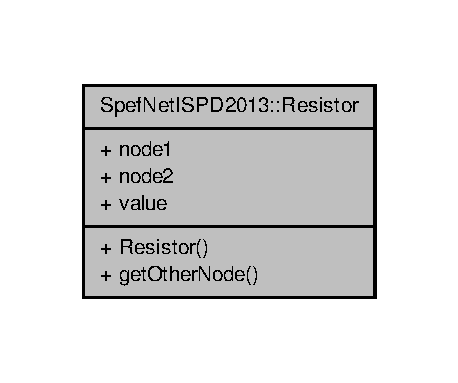
\includegraphics[width=220pt]{structSpefNetISPD2013_1_1Resistor__coll__graph}
\end{center}
\end{figure}
\subsection*{Public Member Functions}
\begin{DoxyCompactItemize}
\item 
\hyperlink{structSpefNetISPD2013_1_1Resistor_ac84e89149ed6b112e9c7f65d6970eedc}{Resistor} (const int \&\hyperlink{structSpefNetISPD2013_1_1Resistor_a3916280dff15e9c4bccafdaba9d40bac}{node1}, const int \&\hyperlink{structSpefNetISPD2013_1_1Resistor_a7da9cba467501e28de314d284c3cf000}{node2}, const double \&\hyperlink{structSpefNetISPD2013_1_1Resistor_aa63c1d820917f71cd4ff2cbf1e83696d}{value})
\begin{DoxyCompactList}\small\item\em \hyperlink{structSpefNetISPD2013_1_1Resistor}{Resistor} constructor. \end{DoxyCompactList}\item 
int \hyperlink{structSpefNetISPD2013_1_1Resistor_a3a0476c9c8c01861071eb667cc79ca22}{get\-Other\-Node} (const int \&node) const 
\begin{DoxyCompactList}\small\item\em If called by node1, returns node2, and vice versa. \end{DoxyCompactList}\end{DoxyCompactItemize}
\subsection*{Public Attributes}
\begin{DoxyCompactItemize}
\item 
int \hyperlink{structSpefNetISPD2013_1_1Resistor_a3916280dff15e9c4bccafdaba9d40bac}{node1}
\item 
int \hyperlink{structSpefNetISPD2013_1_1Resistor_a7da9cba467501e28de314d284c3cf000}{node2}
\item 
double \hyperlink{structSpefNetISPD2013_1_1Resistor_aa63c1d820917f71cd4ff2cbf1e83696d}{value}
\end{DoxyCompactItemize}


\subsection{Detailed Description}
Struct which represents a resistor. 



\subsection{Constructor \& Destructor Documentation}
\hypertarget{structSpefNetISPD2013_1_1Resistor_ac84e89149ed6b112e9c7f65d6970eedc}{\index{Spef\-Net\-I\-S\-P\-D2013\-::\-Resistor@{Spef\-Net\-I\-S\-P\-D2013\-::\-Resistor}!Resistor@{Resistor}}
\index{Resistor@{Resistor}!SpefNetISPD2013::Resistor@{Spef\-Net\-I\-S\-P\-D2013\-::\-Resistor}}
\subsubsection[{Resistor}]{\setlength{\rightskip}{0pt plus 5cm}Spef\-Net\-I\-S\-P\-D2013\-::\-Resistor\-::\-Resistor (
\begin{DoxyParamCaption}
\item[{const int \&}]{node1, }
\item[{const int \&}]{node2, }
\item[{const double \&}]{value}
\end{DoxyParamCaption}
)\hspace{0.3cm}{\ttfamily [inline]}}}\label{structSpefNetISPD2013_1_1Resistor_ac84e89149ed6b112e9c7f65d6970eedc}


\hyperlink{structSpefNetISPD2013_1_1Resistor}{Resistor} constructor. 


\begin{DoxyParams}{Parameters}
{\em const} & string \& node1, const string \& node2, const double \& value \\
\hline
\end{DoxyParams}


\subsection{Member Function Documentation}
\hypertarget{structSpefNetISPD2013_1_1Resistor_a3a0476c9c8c01861071eb667cc79ca22}{\index{Spef\-Net\-I\-S\-P\-D2013\-::\-Resistor@{Spef\-Net\-I\-S\-P\-D2013\-::\-Resistor}!get\-Other\-Node@{get\-Other\-Node}}
\index{get\-Other\-Node@{get\-Other\-Node}!SpefNetISPD2013::Resistor@{Spef\-Net\-I\-S\-P\-D2013\-::\-Resistor}}
\subsubsection[{get\-Other\-Node}]{\setlength{\rightskip}{0pt plus 5cm}int Spef\-Net\-I\-S\-P\-D2013\-::\-Resistor\-::get\-Other\-Node (
\begin{DoxyParamCaption}
\item[{const int \&}]{node}
\end{DoxyParamCaption}
) const\hspace{0.3cm}{\ttfamily [inline]}}}\label{structSpefNetISPD2013_1_1Resistor_a3a0476c9c8c01861071eb667cc79ca22}


If called by node1, returns node2, and vice versa. 


\begin{DoxyParams}{Parameters}
{\em const} & string \& node1, const string \& node2, const double \& value\\
\hline
\end{DoxyParams}
\begin{DoxyReturn}{Returns}
int 
\end{DoxyReturn}


\subsection{Member Data Documentation}
\hypertarget{structSpefNetISPD2013_1_1Resistor_a3916280dff15e9c4bccafdaba9d40bac}{\index{Spef\-Net\-I\-S\-P\-D2013\-::\-Resistor@{Spef\-Net\-I\-S\-P\-D2013\-::\-Resistor}!node1@{node1}}
\index{node1@{node1}!SpefNetISPD2013::Resistor@{Spef\-Net\-I\-S\-P\-D2013\-::\-Resistor}}
\subsubsection[{node1}]{\setlength{\rightskip}{0pt plus 5cm}int Spef\-Net\-I\-S\-P\-D2013\-::\-Resistor\-::node1}}\label{structSpefNetISPD2013_1_1Resistor_a3916280dff15e9c4bccafdaba9d40bac}
\hypertarget{structSpefNetISPD2013_1_1Resistor_a7da9cba467501e28de314d284c3cf000}{\index{Spef\-Net\-I\-S\-P\-D2013\-::\-Resistor@{Spef\-Net\-I\-S\-P\-D2013\-::\-Resistor}!node2@{node2}}
\index{node2@{node2}!SpefNetISPD2013::Resistor@{Spef\-Net\-I\-S\-P\-D2013\-::\-Resistor}}
\subsubsection[{node2}]{\setlength{\rightskip}{0pt plus 5cm}int Spef\-Net\-I\-S\-P\-D2013\-::\-Resistor\-::node2}}\label{structSpefNetISPD2013_1_1Resistor_a7da9cba467501e28de314d284c3cf000}
\hypertarget{structSpefNetISPD2013_1_1Resistor_aa63c1d820917f71cd4ff2cbf1e83696d}{\index{Spef\-Net\-I\-S\-P\-D2013\-::\-Resistor@{Spef\-Net\-I\-S\-P\-D2013\-::\-Resistor}!value@{value}}
\index{value@{value}!SpefNetISPD2013::Resistor@{Spef\-Net\-I\-S\-P\-D2013\-::\-Resistor}}
\subsubsection[{value}]{\setlength{\rightskip}{0pt plus 5cm}double Spef\-Net\-I\-S\-P\-D2013\-::\-Resistor\-::value}}\label{structSpefNetISPD2013_1_1Resistor_aa63c1d820917f71cd4ff2cbf1e83696d}


The documentation for this struct was generated from the following file\-:\begin{DoxyCompactItemize}
\item 
Timing\-Analysis/src/include/\hyperlink{spef__net_8h}{spef\-\_\-net.\-h}\end{DoxyCompactItemize}

\hypertarget{classSDCParser}{\section{S\-D\-C\-Parser Class Reference}
\label{classSDCParser}\index{S\-D\-C\-Parser@{S\-D\-C\-Parser}}
}


Inherits from \hyperlink{classParser}{Parser}. S\-D\-C stands for Synopsys Design Constraints. Used to generate a \hyperlink{classDesign__Constraints}{Design\-\_\-\-Constraints} object from file.  




{\ttfamily \#include $<$parser.\-h$>$}



Inheritance diagram for S\-D\-C\-Parser\-:\nopagebreak
\begin{figure}[H]
\begin{center}
\leavevmode
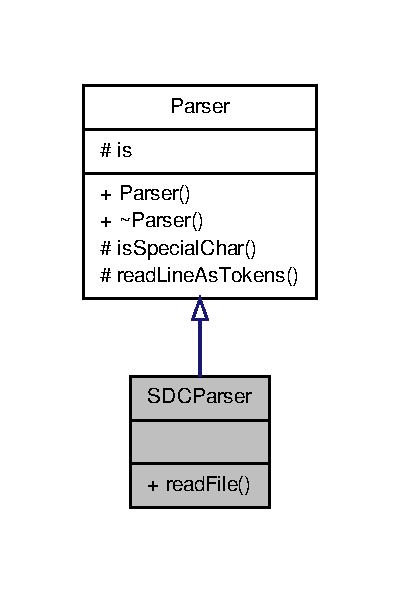
\includegraphics[width=192pt]{classSDCParser__inherit__graph}
\end{center}
\end{figure}


Collaboration diagram for S\-D\-C\-Parser\-:\nopagebreak
\begin{figure}[H]
\begin{center}
\leavevmode
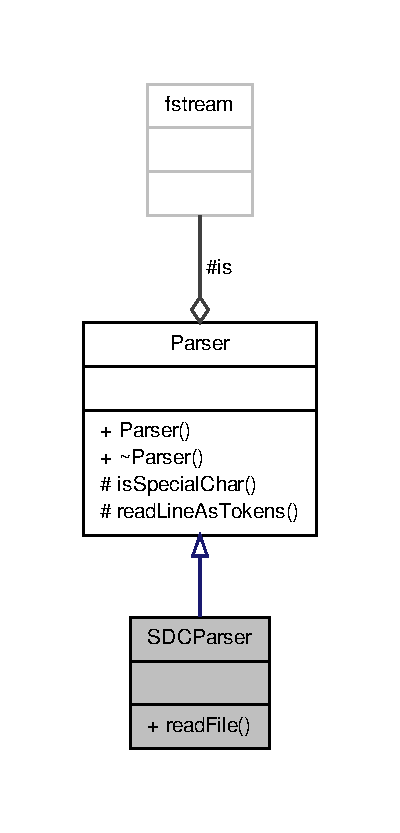
\includegraphics[width=192pt]{classSDCParser__coll__graph}
\end{center}
\end{figure}
\subsection*{Public Member Functions}
\begin{DoxyCompactItemize}
\item 
const \hyperlink{classDesign__Constraints}{Design\-\_\-\-Constraints} \hyperlink{classSDCParser_afc0ae26ac89138dd7b84e2986375785f}{read\-File} (const string filename)
\begin{DoxyCompactList}\small\item\em Returns \hyperlink{classDesign__Constraints}{Design\-\_\-\-Constraints} object generated using informations read from file passed as filename parameter. \end{DoxyCompactList}\end{DoxyCompactItemize}
\subsection*{Additional Inherited Members}


\subsection{Detailed Description}
Inherits from \hyperlink{classParser}{Parser}. S\-D\-C stands for Synopsys Design Constraints. Used to generate a \hyperlink{classDesign__Constraints}{Design\-\_\-\-Constraints} object from file. 

\subsection{Member Function Documentation}
\hypertarget{classSDCParser_afc0ae26ac89138dd7b84e2986375785f}{\index{S\-D\-C\-Parser@{S\-D\-C\-Parser}!read\-File@{read\-File}}
\index{read\-File@{read\-File}!SDCParser@{S\-D\-C\-Parser}}
\subsubsection[{read\-File}]{\setlength{\rightskip}{0pt plus 5cm}const {\bf Design\-\_\-\-Constraints} S\-D\-C\-Parser\-::read\-File (
\begin{DoxyParamCaption}
\item[{const string}]{filename}
\end{DoxyParamCaption}
)}}\label{classSDCParser_afc0ae26ac89138dd7b84e2986375785f}


Returns \hyperlink{classDesign__Constraints}{Design\-\_\-\-Constraints} object generated using informations read from file passed as filename parameter. 


\begin{DoxyParams}{Parameters}
{\em const} & string filename\\
\hline
\end{DoxyParams}
\begin{DoxyReturn}{Returns}
const \hyperlink{classDesign__Constraints}{Design\-\_\-\-Constraints} 
\end{DoxyReturn}


The documentation for this class was generated from the following file\-:\begin{DoxyCompactItemize}
\item 
Timing\-Analysis/src/include/\hyperlink{parser_8h}{parser.\-h}\end{DoxyCompactItemize}

\hypertarget{classTiming__Analysis_1_1Single__Fanout__Edge}{\section{Timing\-\_\-\-Analysis\-:\-:Single\-\_\-\-Fanout\-\_\-\-Edge$<$ T $>$ Class Template Reference}
\label{classTiming__Analysis_1_1Single__Fanout__Edge}\index{Timing\-\_\-\-Analysis\-::\-Single\-\_\-\-Fanout\-\_\-\-Edge$<$ T $>$@{Timing\-\_\-\-Analysis\-::\-Single\-\_\-\-Fanout\-\_\-\-Edge$<$ T $>$}}
}


Inherits from \hyperlink{classTiming__Analysis_1_1Edge}{Edge}. A single fanout edge is an edge which two vertex to each other.  




{\ttfamily \#include $<$single\-\_\-fanout\-\_\-edge.\-h$>$}

Inheritance diagram for Timing\-\_\-\-Analysis\-:\-:Single\-\_\-\-Fanout\-\_\-\-Edge$<$ T $>$\-:\begin{figure}[H]
\begin{center}
\leavevmode
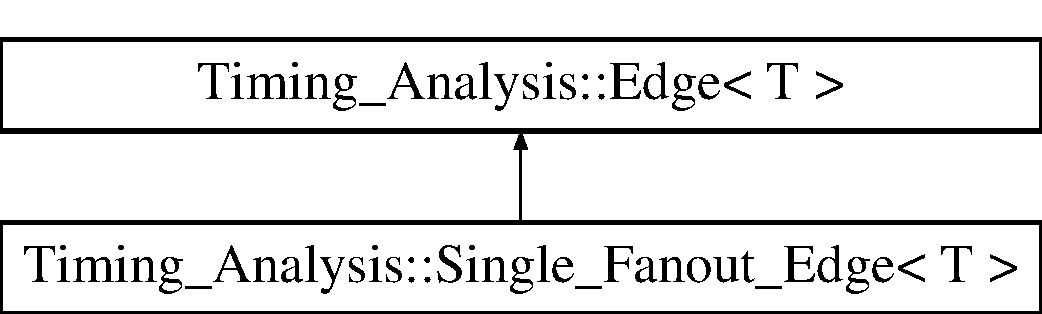
\includegraphics[height=2.000000cm]{classTiming__Analysis_1_1Single__Fanout__Edge}
\end{center}
\end{figure}
\subsection*{Public Member Functions}
\begin{DoxyCompactItemize}
\item 
\hyperlink{classTiming__Analysis_1_1Single__Fanout__Edge_ac588152ff213288a57a744374039790a}{Single\-\_\-\-Fanout\-\_\-\-Edge} (T $\ast$\hyperlink{classTiming__Analysis_1_1Edge_a47020ea89fd9fde438adc814a731a23d}{from}, T $\ast$\hyperlink{classTiming__Analysis_1_1Single__Fanout__Edge_ac01deccce158b6cee6883924e6dcb788}{to})
\begin{DoxyCompactList}\small\item\em \hyperlink{classTiming__Analysis_1_1Single__Fanout__Edge}{Single\-\_\-\-Fanout\-\_\-\-Edge} constructor. \end{DoxyCompactList}\item 
T \& \hyperlink{classTiming__Analysis_1_1Single__Fanout__Edge_ac01deccce158b6cee6883924e6dcb788}{to} (void) const 
\begin{DoxyCompactList}\small\item\em Returns Edge$<$\-T$>$ \end{DoxyCompactList}\end{DoxyCompactItemize}
\subsection*{Additional Inherited Members}


\subsection{Detailed Description}
\subsubsection*{template$<$class T$>$class Timing\-\_\-\-Analysis\-::\-Single\-\_\-\-Fanout\-\_\-\-Edge$<$ T $>$}

Inherits from \hyperlink{classTiming__Analysis_1_1Edge}{Edge}. A single fanout edge is an edge which two vertex to each other. 



\subsection{Constructor \& Destructor Documentation}
\hypertarget{classTiming__Analysis_1_1Single__Fanout__Edge_ac588152ff213288a57a744374039790a}{\index{Timing\-\_\-\-Analysis\-::\-Single\-\_\-\-Fanout\-\_\-\-Edge@{Timing\-\_\-\-Analysis\-::\-Single\-\_\-\-Fanout\-\_\-\-Edge}!Single\-\_\-\-Fanout\-\_\-\-Edge@{Single\-\_\-\-Fanout\-\_\-\-Edge}}
\index{Single\-\_\-\-Fanout\-\_\-\-Edge@{Single\-\_\-\-Fanout\-\_\-\-Edge}!Timing_Analysis::Single_Fanout_Edge@{Timing\-\_\-\-Analysis\-::\-Single\-\_\-\-Fanout\-\_\-\-Edge}}
\subsubsection[{Single\-\_\-\-Fanout\-\_\-\-Edge}]{\setlength{\rightskip}{0pt plus 5cm}template$<$class T$>$ {\bf Timing\-\_\-\-Analysis\-::\-Single\-\_\-\-Fanout\-\_\-\-Edge}$<$ T $>$\-::{\bf Single\-\_\-\-Fanout\-\_\-\-Edge} (
\begin{DoxyParamCaption}
\item[{T $\ast$}]{from, }
\item[{T $\ast$}]{to}
\end{DoxyParamCaption}
)\hspace{0.3cm}{\ttfamily [inline]}}}\label{classTiming__Analysis_1_1Single__Fanout__Edge_ac588152ff213288a57a744374039790a}


\hyperlink{classTiming__Analysis_1_1Single__Fanout__Edge}{Single\-\_\-\-Fanout\-\_\-\-Edge} constructor. 



\subsection{Member Function Documentation}
\hypertarget{classTiming__Analysis_1_1Single__Fanout__Edge_ac01deccce158b6cee6883924e6dcb788}{\index{Timing\-\_\-\-Analysis\-::\-Single\-\_\-\-Fanout\-\_\-\-Edge@{Timing\-\_\-\-Analysis\-::\-Single\-\_\-\-Fanout\-\_\-\-Edge}!to@{to}}
\index{to@{to}!Timing_Analysis::Single_Fanout_Edge@{Timing\-\_\-\-Analysis\-::\-Single\-\_\-\-Fanout\-\_\-\-Edge}}
\subsubsection[{to}]{\setlength{\rightskip}{0pt plus 5cm}template$<$class T$>$ T\& {\bf Timing\-\_\-\-Analysis\-::\-Single\-\_\-\-Fanout\-\_\-\-Edge}$<$ T $>$\-::to (
\begin{DoxyParamCaption}
\item[{void}]{}
\end{DoxyParamCaption}
) const\hspace{0.3cm}{\ttfamily [inline]}}}\label{classTiming__Analysis_1_1Single__Fanout__Edge_ac01deccce158b6cee6883924e6dcb788}


Returns Edge$<$\-T$>$ 

\begin{DoxyReturn}{Returns}
T \& 
\end{DoxyReturn}


The documentation for this class was generated from the following file\-:\begin{DoxyCompactItemize}
\item 
tcc\-Chrystian/src/include/single\-\_\-fanout\-\_\-edge.\-h\end{DoxyCompactItemize}

\hypertarget{structCircuit__Netlist_1_1Sink}{\section{Circuit\-\_\-\-Netlist\-:\-:Sink Struct Reference}
\label{structCircuit__Netlist_1_1Sink}\index{Circuit\-\_\-\-Netlist\-::\-Sink@{Circuit\-\_\-\-Netlist\-::\-Sink}}
}


Struct which represents a \hyperlink{structCircuit__Netlist_1_1Sink}{Sink}. A sink is a vertex which has input edges, but no output edges(outdegree zerp).  




{\ttfamily \#include $<$circuit\-\_\-netlist.\-h$>$}

\subsection*{Public Member Functions}
\begin{DoxyCompactItemize}
\item 
\hyperlink{structCircuit__Netlist_1_1Sink_ad56d7d6a65455ec3e328d4bb8876936f}{Sink} (const int gate, const string pin\-Name)
\begin{DoxyCompactList}\small\item\em \hyperlink{structCircuit__Netlist_1_1Sink}{Sink} constructor. \end{DoxyCompactList}\end{DoxyCompactItemize}
\subsection*{Public Attributes}
\begin{DoxyCompactItemize}
\item 
\hypertarget{structCircuit__Netlist_1_1Sink_a5728898bf1ef8a37b46f0f6274676889}{int {\bfseries gate}}\label{structCircuit__Netlist_1_1Sink_a5728898bf1ef8a37b46f0f6274676889}

\item 
\hypertarget{structCircuit__Netlist_1_1Sink_ac2072a83f3d654b10f6ad0b2049cc2e6}{string {\bfseries pin\-Name}}\label{structCircuit__Netlist_1_1Sink_ac2072a83f3d654b10f6ad0b2049cc2e6}

\end{DoxyCompactItemize}


\subsection{Detailed Description}
Struct which represents a \hyperlink{structCircuit__Netlist_1_1Sink}{Sink}. A sink is a vertex which has input edges, but no output edges(outdegree zerp). 



\subsection{Constructor \& Destructor Documentation}
\hypertarget{structCircuit__Netlist_1_1Sink_ad56d7d6a65455ec3e328d4bb8876936f}{\index{Circuit\-\_\-\-Netlist\-::\-Sink@{Circuit\-\_\-\-Netlist\-::\-Sink}!Sink@{Sink}}
\index{Sink@{Sink}!Circuit_Netlist::Sink@{Circuit\-\_\-\-Netlist\-::\-Sink}}
\subsubsection[{Sink}]{\setlength{\rightskip}{0pt plus 5cm}Circuit\-\_\-\-Netlist\-::\-Sink\-::\-Sink (
\begin{DoxyParamCaption}
\item[{const int}]{gate, }
\item[{const string}]{pin\-Name}
\end{DoxyParamCaption}
)\hspace{0.3cm}{\ttfamily [inline]}}}\label{structCircuit__Netlist_1_1Sink_ad56d7d6a65455ec3e328d4bb8876936f}


\hyperlink{structCircuit__Netlist_1_1Sink}{Sink} constructor. 


\begin{DoxyParams}{Parameters}
{\em const} & int gate, const string pin\-Name \\
\hline
\end{DoxyParams}


The documentation for this struct was generated from the following file\-:\begin{DoxyCompactItemize}
\item 
tcc\-Chrystian/src/include/circuit\-\_\-netlist.\-h\end{DoxyCompactItemize}

\hypertarget{classSpefNetISPD2012}{\section{Spef\-Net\-I\-S\-P\-D2012 Class Reference}
\label{classSpefNetISPD2012}\index{Spef\-Net\-I\-S\-P\-D2012@{Spef\-Net\-I\-S\-P\-D2012}}
}


S\-P\-E\-F stands for Standard Parasitic Exchange Format. Describes the set of parasitic elements of the wires in a circuit, within its descriptions and values. Generated by \hyperlink{classSpefParserISPD2012}{Spef\-Parser\-I\-S\-P\-D2012}.  




{\ttfamily \#include $<$spef\-\_\-net.\-h$>$}

\subsection*{Public Attributes}
\begin{DoxyCompactItemize}
\item 
\hypertarget{classSpefNetISPD2012_aed87a4b73a2ad09be841c9b8ab222ad5}{string {\bfseries net\-Name}}\label{classSpefNetISPD2012_aed87a4b73a2ad09be841c9b8ab222ad5}

\item 
\hypertarget{classSpefNetISPD2012_ae0a1b7a236104b7a6be70fc977fe20e7}{double {\bfseries net\-Lumped\-Cap}}\label{classSpefNetISPD2012_ae0a1b7a236104b7a6be70fc977fe20e7}

\end{DoxyCompactItemize}


\subsection{Detailed Description}
S\-P\-E\-F stands for Standard Parasitic Exchange Format. Describes the set of parasitic elements of the wires in a circuit, within its descriptions and values. Generated by \hyperlink{classSpefParserISPD2012}{Spef\-Parser\-I\-S\-P\-D2012}. 



The documentation for this class was generated from the following file\-:\begin{DoxyCompactItemize}
\item 
tcc\-Chrystian/src/include/spef\-\_\-net.\-h\end{DoxyCompactItemize}

\hypertarget{classSpefNetISPD2013}{\section{Spef\-Net\-I\-S\-P\-D2013 Class Reference}
\label{classSpefNetISPD2013}\index{Spef\-Net\-I\-S\-P\-D2013@{Spef\-Net\-I\-S\-P\-D2013}}
}


S\-P\-E\-F stands for Standard Parasitic Exchange Format. Describes the set of parasitic elements of the wires in a circuit, within its descriptions and values.  




{\ttfamily \#include $<$spef\-\_\-net.\-h$>$}

\subsection*{Classes}
\begin{DoxyCompactItemize}
\item 
struct \hyperlink{structSpefNetISPD2013_1_1Capacitor}{Capacitor}
\begin{DoxyCompactList}\small\item\em Struct which represents a capacitor. \end{DoxyCompactList}\item 
struct \hyperlink{structSpefNetISPD2013_1_1Node}{Node}
\begin{DoxyCompactList}\small\item\em Struct which represents a node of the circuit. A node is a point of the circuit where two or more elements meet. \end{DoxyCompactList}\item 
struct \hyperlink{structSpefNetISPD2013_1_1Resistor}{Resistor}
\begin{DoxyCompactList}\small\item\em Struct which represents a resistor. \end{DoxyCompactList}\end{DoxyCompactItemize}
\subsection*{Public Member Functions}
\begin{DoxyCompactItemize}
\item 
\hyperlink{classSpefNetISPD2013_a41ab1d666a3724e63e0fd815765f1372}{Spef\-Net\-I\-S\-P\-D2013} ()
\begin{DoxyCompactList}\small\item\em Empty Spef\-Net constructor. \end{DoxyCompactList}\item 
virtual \hyperlink{classSpefNetISPD2013_a6bd1c7cc6d7bdf677fb69bb577a6327f}{$\sim$\-Spef\-Net\-I\-S\-P\-D2013} ()
\begin{DoxyCompactList}\small\item\em Empty Spef\-Net destructor. \end{DoxyCompactList}\item 
void \hyperlink{classSpefNetISPD2013_ac837ca5049dd0fc8301b1c51a8508bfd}{add\-Resistor} (const string \&node1, const string \&node2, const double \&value)
\begin{DoxyCompactList}\small\item\em Adds new resistor to nodes/resistors list. \end{DoxyCompactList}\item 
void \hyperlink{classSpefNetISPD2013_a9d5344541f303241af6bec439a692850}{add\-Capacitor} (const string \&node, const double \&value)
\begin{DoxyCompactList}\small\item\em Adds new capacitor to nodes/capacitors list. \end{DoxyCompactList}\item 
size\-\_\-t \hyperlink{classSpefNetISPD2013_a68ae22df2961b88537802d444dd20588}{nodes\-Size} () const 
\begin{DoxyCompactList}\small\item\em Returns number of nodes. \end{DoxyCompactList}\item 
const \hyperlink{structSpefNetISPD2013_1_1Node}{Node} \& \hyperlink{classSpefNetISPD2013_a8beeae8a280358ba32eedab9367b1006}{get\-Node} (const unsigned \&i) const 
\begin{DoxyCompactList}\small\item\em Gets node at index i. \end{DoxyCompactList}\item 
int \hyperlink{classSpefNetISPD2013_aa5143da0b98e3fa1613562061238f4ee}{get\-Node\-Index} (const string \&name) const 
\begin{DoxyCompactList}\small\item\em Returns index of node name. If not found, returns -\/1. \end{DoxyCompactList}\item 
size\-\_\-t \hyperlink{classSpefNetISPD2013_a1a15314aec6fae289f90b9e7de201fe8}{resistors\-Size} () const 
\begin{DoxyCompactList}\small\item\em Retuns number of resistors. \end{DoxyCompactList}\item 
const \hyperlink{structSpefNetISPD2013_1_1Resistor}{Resistor} \& \hyperlink{classSpefNetISPD2013_a1baa70cdf4b2c65a7e695849c2ad2525}{get\-Resistor} (const unsigned \&i) const 
\begin{DoxyCompactList}\small\item\em Returns resistor at index i. \end{DoxyCompactList}\item 
void \hyperlink{classSpefNetISPD2013_a3a0ed208b150100bda0544112fb1c0ba}{set} (string name, double lumped\-Capacitance)
\begin{DoxyCompactList}\small\item\em Sets S\-P\-E\-F netlist atributtes. \end{DoxyCompactList}\end{DoxyCompactItemize}
\subsection*{Public Attributes}
\begin{DoxyCompactItemize}
\item 
\hypertarget{classSpefNetISPD2013_a1aa3f32d0cac9a7b1800ab67903361fa}{string {\bfseries net\-Name}}\label{classSpefNetISPD2013_a1aa3f32d0cac9a7b1800ab67903361fa}

\item 
\hypertarget{classSpefNetISPD2013_af088c8d7cbca748a4a56ab796ccb2fd5}{double {\bfseries net\-Lumped\-Cap}}\label{classSpefNetISPD2013_af088c8d7cbca748a4a56ab796ccb2fd5}

\end{DoxyCompactItemize}
\subsection*{Friends}
\begin{DoxyCompactItemize}
\item 
ostream \& \hyperlink{classSpefNetISPD2013_a6a52417a5250abf94d511910add3415e}{operator$<$$<$} (ostream \&out, const \hyperlink{classSpefNetISPD2013}{Spef\-Net\-I\-S\-P\-D2013} \&descriptor)
\begin{DoxyCompactList}\small\item\em Redefinition of $<$$<$ operator. Inserts description including node name, index, capacitance and resistances list. \end{DoxyCompactList}\end{DoxyCompactItemize}


\subsection{Detailed Description}
S\-P\-E\-F stands for Standard Parasitic Exchange Format. Describes the set of parasitic elements of the wires in a circuit, within its descriptions and values. 



\subsection{Constructor \& Destructor Documentation}
\hypertarget{classSpefNetISPD2013_a41ab1d666a3724e63e0fd815765f1372}{\index{Spef\-Net\-I\-S\-P\-D2013@{Spef\-Net\-I\-S\-P\-D2013}!Spef\-Net\-I\-S\-P\-D2013@{Spef\-Net\-I\-S\-P\-D2013}}
\index{Spef\-Net\-I\-S\-P\-D2013@{Spef\-Net\-I\-S\-P\-D2013}!SpefNetISPD2013@{Spef\-Net\-I\-S\-P\-D2013}}
\subsubsection[{Spef\-Net\-I\-S\-P\-D2013}]{\setlength{\rightskip}{0pt plus 5cm}Spef\-Net\-I\-S\-P\-D2013\-::\-Spef\-Net\-I\-S\-P\-D2013 (
\begin{DoxyParamCaption}
{}
\end{DoxyParamCaption}
)\hspace{0.3cm}{\ttfamily [inline]}}}\label{classSpefNetISPD2013_a41ab1d666a3724e63e0fd815765f1372}


Empty Spef\-Net constructor. 

\hypertarget{classSpefNetISPD2013_a6bd1c7cc6d7bdf677fb69bb577a6327f}{\index{Spef\-Net\-I\-S\-P\-D2013@{Spef\-Net\-I\-S\-P\-D2013}!$\sim$\-Spef\-Net\-I\-S\-P\-D2013@{$\sim$\-Spef\-Net\-I\-S\-P\-D2013}}
\index{$\sim$\-Spef\-Net\-I\-S\-P\-D2013@{$\sim$\-Spef\-Net\-I\-S\-P\-D2013}!SpefNetISPD2013@{Spef\-Net\-I\-S\-P\-D2013}}
\subsubsection[{$\sim$\-Spef\-Net\-I\-S\-P\-D2013}]{\setlength{\rightskip}{0pt plus 5cm}virtual Spef\-Net\-I\-S\-P\-D2013\-::$\sim$\-Spef\-Net\-I\-S\-P\-D2013 (
\begin{DoxyParamCaption}
{}
\end{DoxyParamCaption}
)\hspace{0.3cm}{\ttfamily [inline]}, {\ttfamily [virtual]}}}\label{classSpefNetISPD2013_a6bd1c7cc6d7bdf677fb69bb577a6327f}


Empty Spef\-Net destructor. 



\subsection{Member Function Documentation}
\hypertarget{classSpefNetISPD2013_a9d5344541f303241af6bec439a692850}{\index{Spef\-Net\-I\-S\-P\-D2013@{Spef\-Net\-I\-S\-P\-D2013}!add\-Capacitor@{add\-Capacitor}}
\index{add\-Capacitor@{add\-Capacitor}!SpefNetISPD2013@{Spef\-Net\-I\-S\-P\-D2013}}
\subsubsection[{add\-Capacitor}]{\setlength{\rightskip}{0pt plus 5cm}void Spef\-Net\-I\-S\-P\-D2013\-::add\-Capacitor (
\begin{DoxyParamCaption}
\item[{const string \&}]{node, }
\item[{const double \&}]{value}
\end{DoxyParamCaption}
)}}\label{classSpefNetISPD2013_a9d5344541f303241af6bec439a692850}


Adds new capacitor to nodes/capacitors list. 


\begin{DoxyParams}{Parameters}
{\em const} & string \& node, const double \& value\\
\hline
\end{DoxyParams}
\begin{DoxyReturn}{Returns}
void 
\end{DoxyReturn}
\hypertarget{classSpefNetISPD2013_ac837ca5049dd0fc8301b1c51a8508bfd}{\index{Spef\-Net\-I\-S\-P\-D2013@{Spef\-Net\-I\-S\-P\-D2013}!add\-Resistor@{add\-Resistor}}
\index{add\-Resistor@{add\-Resistor}!SpefNetISPD2013@{Spef\-Net\-I\-S\-P\-D2013}}
\subsubsection[{add\-Resistor}]{\setlength{\rightskip}{0pt plus 5cm}void Spef\-Net\-I\-S\-P\-D2013\-::add\-Resistor (
\begin{DoxyParamCaption}
\item[{const string \&}]{node1, }
\item[{const string \&}]{node2, }
\item[{const double \&}]{value}
\end{DoxyParamCaption}
)}}\label{classSpefNetISPD2013_ac837ca5049dd0fc8301b1c51a8508bfd}


Adds new resistor to nodes/resistors list. 


\begin{DoxyParams}{Parameters}
{\em const} & string \& node1, const string \& node2, const double \& value\\
\hline
\end{DoxyParams}
\begin{DoxyReturn}{Returns}
void 
\end{DoxyReturn}
\hypertarget{classSpefNetISPD2013_a8beeae8a280358ba32eedab9367b1006}{\index{Spef\-Net\-I\-S\-P\-D2013@{Spef\-Net\-I\-S\-P\-D2013}!get\-Node@{get\-Node}}
\index{get\-Node@{get\-Node}!SpefNetISPD2013@{Spef\-Net\-I\-S\-P\-D2013}}
\subsubsection[{get\-Node}]{\setlength{\rightskip}{0pt plus 5cm}const {\bf Node}\& Spef\-Net\-I\-S\-P\-D2013\-::get\-Node (
\begin{DoxyParamCaption}
\item[{const unsigned \&}]{i}
\end{DoxyParamCaption}
) const\hspace{0.3cm}{\ttfamily [inline]}}}\label{classSpefNetISPD2013_a8beeae8a280358ba32eedab9367b1006}


Gets node at index i. 


\begin{DoxyParams}{Parameters}
{\em const} & unsigned \& i\\
\hline
\end{DoxyParams}
\begin{DoxyReturn}{Returns}
const \hyperlink{structSpefNetISPD2013_1_1Node}{Node} 
\end{DoxyReturn}
\hypertarget{classSpefNetISPD2013_aa5143da0b98e3fa1613562061238f4ee}{\index{Spef\-Net\-I\-S\-P\-D2013@{Spef\-Net\-I\-S\-P\-D2013}!get\-Node\-Index@{get\-Node\-Index}}
\index{get\-Node\-Index@{get\-Node\-Index}!SpefNetISPD2013@{Spef\-Net\-I\-S\-P\-D2013}}
\subsubsection[{get\-Node\-Index}]{\setlength{\rightskip}{0pt plus 5cm}int Spef\-Net\-I\-S\-P\-D2013\-::get\-Node\-Index (
\begin{DoxyParamCaption}
\item[{const string \&}]{name}
\end{DoxyParamCaption}
) const}}\label{classSpefNetISPD2013_aa5143da0b98e3fa1613562061238f4ee}


Returns index of node name. If not found, returns -\/1. 


\begin{DoxyParams}{Parameters}
{\em const} & string \& name\\
\hline
\end{DoxyParams}
\begin{DoxyReturn}{Returns}
int 
\end{DoxyReturn}
\hypertarget{classSpefNetISPD2013_a1baa70cdf4b2c65a7e695849c2ad2525}{\index{Spef\-Net\-I\-S\-P\-D2013@{Spef\-Net\-I\-S\-P\-D2013}!get\-Resistor@{get\-Resistor}}
\index{get\-Resistor@{get\-Resistor}!SpefNetISPD2013@{Spef\-Net\-I\-S\-P\-D2013}}
\subsubsection[{get\-Resistor}]{\setlength{\rightskip}{0pt plus 5cm}const {\bf Resistor}\& Spef\-Net\-I\-S\-P\-D2013\-::get\-Resistor (
\begin{DoxyParamCaption}
\item[{const unsigned \&}]{i}
\end{DoxyParamCaption}
) const\hspace{0.3cm}{\ttfamily [inline]}}}\label{classSpefNetISPD2013_a1baa70cdf4b2c65a7e695849c2ad2525}


Returns resistor at index i. 


\begin{DoxyParams}{Parameters}
{\em const} & unsigned \& i\\
\hline
\end{DoxyParams}
\begin{DoxyReturn}{Returns}
const \hyperlink{structSpefNetISPD2013_1_1Resistor}{Resistor} 
\end{DoxyReturn}
\hypertarget{classSpefNetISPD2013_a68ae22df2961b88537802d444dd20588}{\index{Spef\-Net\-I\-S\-P\-D2013@{Spef\-Net\-I\-S\-P\-D2013}!nodes\-Size@{nodes\-Size}}
\index{nodes\-Size@{nodes\-Size}!SpefNetISPD2013@{Spef\-Net\-I\-S\-P\-D2013}}
\subsubsection[{nodes\-Size}]{\setlength{\rightskip}{0pt plus 5cm}size\-\_\-t Spef\-Net\-I\-S\-P\-D2013\-::nodes\-Size (
\begin{DoxyParamCaption}
{}
\end{DoxyParamCaption}
) const\hspace{0.3cm}{\ttfamily [inline]}}}\label{classSpefNetISPD2013_a68ae22df2961b88537802d444dd20588}


Returns number of nodes. 

\begin{DoxyReturn}{Returns}
size\-\_\-t 
\end{DoxyReturn}
\hypertarget{classSpefNetISPD2013_a1a15314aec6fae289f90b9e7de201fe8}{\index{Spef\-Net\-I\-S\-P\-D2013@{Spef\-Net\-I\-S\-P\-D2013}!resistors\-Size@{resistors\-Size}}
\index{resistors\-Size@{resistors\-Size}!SpefNetISPD2013@{Spef\-Net\-I\-S\-P\-D2013}}
\subsubsection[{resistors\-Size}]{\setlength{\rightskip}{0pt plus 5cm}size\-\_\-t Spef\-Net\-I\-S\-P\-D2013\-::resistors\-Size (
\begin{DoxyParamCaption}
{}
\end{DoxyParamCaption}
) const\hspace{0.3cm}{\ttfamily [inline]}}}\label{classSpefNetISPD2013_a1a15314aec6fae289f90b9e7de201fe8}


Retuns number of resistors. 

\begin{DoxyReturn}{Returns}
size\-\_\-t 
\end{DoxyReturn}
\hypertarget{classSpefNetISPD2013_a3a0ed208b150100bda0544112fb1c0ba}{\index{Spef\-Net\-I\-S\-P\-D2013@{Spef\-Net\-I\-S\-P\-D2013}!set@{set}}
\index{set@{set}!SpefNetISPD2013@{Spef\-Net\-I\-S\-P\-D2013}}
\subsubsection[{set}]{\setlength{\rightskip}{0pt plus 5cm}void Spef\-Net\-I\-S\-P\-D2013\-::set (
\begin{DoxyParamCaption}
\item[{string}]{name, }
\item[{double}]{lumped\-Capacitance}
\end{DoxyParamCaption}
)}}\label{classSpefNetISPD2013_a3a0ed208b150100bda0544112fb1c0ba}


Sets S\-P\-E\-F netlist atributtes. 


\begin{DoxyParams}{Parameters}
{\em string} & name,double lumped\-Capacitance\\
\hline
\end{DoxyParams}
\begin{DoxyReturn}{Returns}
void 
\end{DoxyReturn}


\subsection{Friends And Related Function Documentation}
\hypertarget{classSpefNetISPD2013_a6a52417a5250abf94d511910add3415e}{\index{Spef\-Net\-I\-S\-P\-D2013@{Spef\-Net\-I\-S\-P\-D2013}!operator$<$$<$@{operator$<$$<$}}
\index{operator$<$$<$@{operator$<$$<$}!SpefNetISPD2013@{Spef\-Net\-I\-S\-P\-D2013}}
\subsubsection[{operator$<$$<$}]{\setlength{\rightskip}{0pt plus 5cm}ostream\& operator$<$$<$ (
\begin{DoxyParamCaption}
\item[{ostream \&}]{out, }
\item[{const {\bf Spef\-Net\-I\-S\-P\-D2013} \&}]{descriptor}
\end{DoxyParamCaption}
)\hspace{0.3cm}{\ttfamily [friend]}}}\label{classSpefNetISPD2013_a6a52417a5250abf94d511910add3415e}


Redefinition of $<$$<$ operator. Inserts description including node name, index, capacitance and resistances list. 



The documentation for this class was generated from the following file\-:\begin{DoxyCompactItemize}
\item 
tcc\-Chrystian/src/include/spef\-\_\-net.\-h\end{DoxyCompactItemize}

\hypertarget{classSpefParserISPD2012}{\section{Spef\-Parser\-I\-S\-P\-D2012 Class Reference}
\label{classSpefParserISPD2012}\index{Spef\-Parser\-I\-S\-P\-D2012@{Spef\-Parser\-I\-S\-P\-D2012}}
}


Inherits from \hyperlink{classParser}{Parser}. Used to generate \hyperlink{classSpefNetISPD2012}{Spef\-Net\-I\-S\-P\-D2012} files from an input.  




{\ttfamily \#include $<$parser.\-h$>$}



Inheritance diagram for Spef\-Parser\-I\-S\-P\-D2012\-:\nopagebreak
\begin{figure}[H]
\begin{center}
\leavevmode
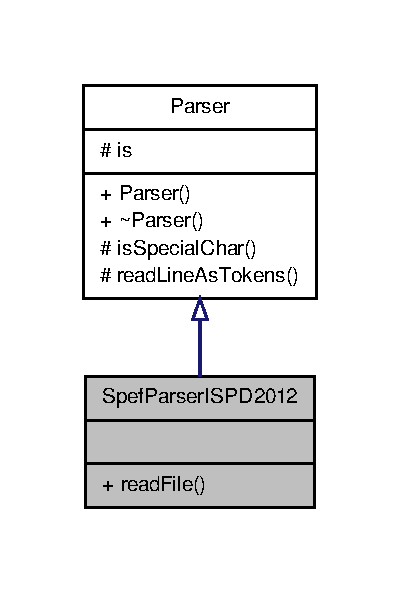
\includegraphics[width=192pt]{classSpefParserISPD2012__inherit__graph}
\end{center}
\end{figure}


Collaboration diagram for Spef\-Parser\-I\-S\-P\-D2012\-:\nopagebreak
\begin{figure}[H]
\begin{center}
\leavevmode
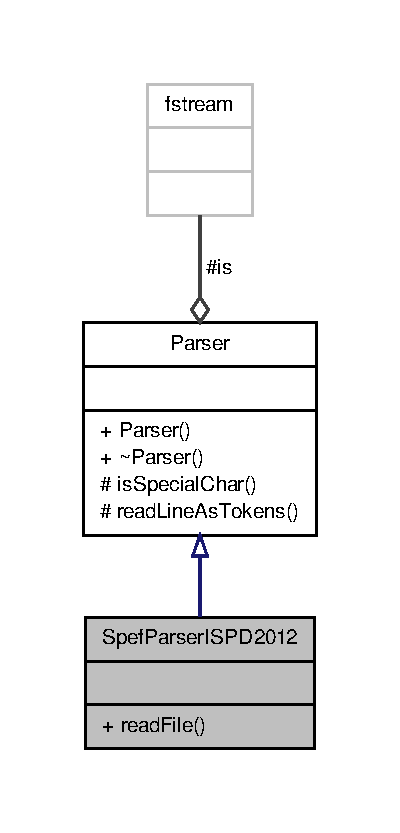
\includegraphics[width=192pt]{classSpefParserISPD2012__coll__graph}
\end{center}
\end{figure}
\subsection*{Public Member Functions}
\begin{DoxyCompactItemize}
\item 
const \hyperlink{spef__net_8h_a37551e9359ee22bb0821ca94784447d4}{Parasitics2012} \hyperlink{classSpefParserISPD2012_a130209fe17a1d791cd03543304e48d5e}{read\-File} (const string filename)
\begin{DoxyCompactList}\small\item\em Returns Parasitics2012 object generated using informations read from file passed as filename parameter. \end{DoxyCompactList}\end{DoxyCompactItemize}
\subsection*{Additional Inherited Members}


\subsection{Detailed Description}
Inherits from \hyperlink{classParser}{Parser}. Used to generate \hyperlink{classSpefNetISPD2012}{Spef\-Net\-I\-S\-P\-D2012} files from an input. 

\subsection{Member Function Documentation}
\hypertarget{classSpefParserISPD2012_a130209fe17a1d791cd03543304e48d5e}{\index{Spef\-Parser\-I\-S\-P\-D2012@{Spef\-Parser\-I\-S\-P\-D2012}!read\-File@{read\-File}}
\index{read\-File@{read\-File}!SpefParserISPD2012@{Spef\-Parser\-I\-S\-P\-D2012}}
\subsubsection[{read\-File}]{\setlength{\rightskip}{0pt plus 5cm}const {\bf Parasitics2012} Spef\-Parser\-I\-S\-P\-D2012\-::read\-File (
\begin{DoxyParamCaption}
\item[{const string}]{filename}
\end{DoxyParamCaption}
)}}\label{classSpefParserISPD2012_a130209fe17a1d791cd03543304e48d5e}


Returns Parasitics2012 object generated using informations read from file passed as filename parameter. 


\begin{DoxyParams}{Parameters}
{\em const} & string filename\\
\hline
\end{DoxyParams}
\begin{DoxyReturn}{Returns}
Parasitics2012 
\end{DoxyReturn}


The documentation for this class was generated from the following file\-:\begin{DoxyCompactItemize}
\item 
Timing\-Analysis/src/include/\hyperlink{parser_8h}{parser.\-h}\end{DoxyCompactItemize}

\hypertarget{classSpefParserISPD2013}{\section{Spef\-Parser\-I\-S\-P\-D2013 Class Reference}
\label{classSpefParserISPD2013}\index{Spef\-Parser\-I\-S\-P\-D2013@{Spef\-Parser\-I\-S\-P\-D2013}}
}


Inherits from \hyperlink{classParser}{Parser}. Used to generate \hyperlink{classSpefNetISPD2013}{Spef\-Net\-I\-S\-P\-D2013} file from an input.  




{\ttfamily \#include $<$parser.\-h$>$}

Inheritance diagram for Spef\-Parser\-I\-S\-P\-D2013\-:\begin{figure}[H]
\begin{center}
\leavevmode
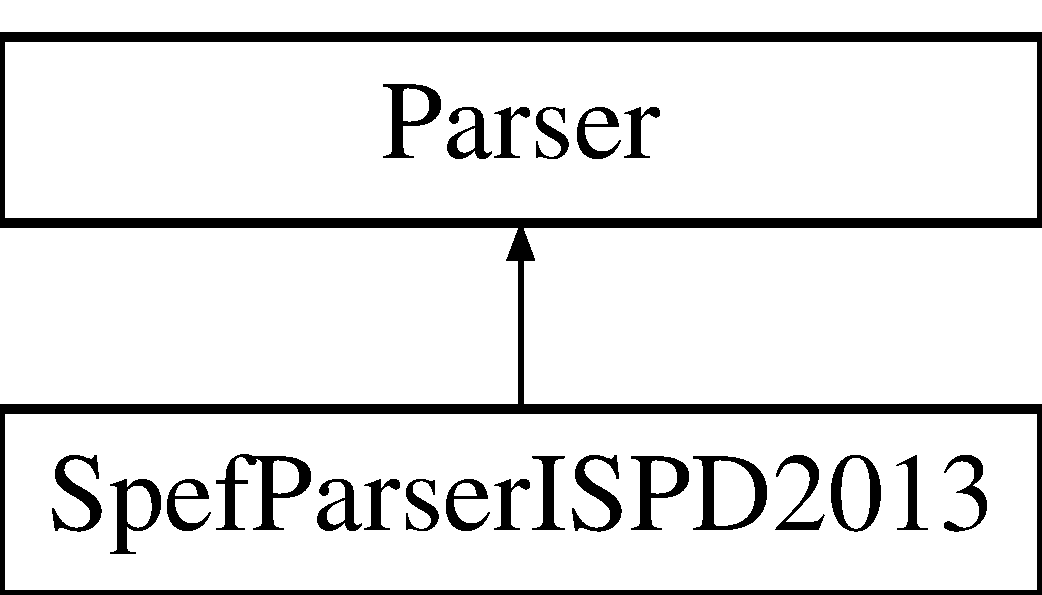
\includegraphics[height=2.000000cm]{classSpefParserISPD2013}
\end{center}
\end{figure}
\subsection*{Public Member Functions}
\begin{DoxyCompactItemize}
\item 
const Parasitics2013 \hyperlink{classSpefParserISPD2013_a11c71d121883895a367a99b052aada73}{read\-File} (const string filename)
\begin{DoxyCompactList}\small\item\em Returns Parasitics2013 object generated using informations read from file passed as filename parameter. \end{DoxyCompactList}\end{DoxyCompactItemize}
\subsection*{Additional Inherited Members}


\subsection{Detailed Description}
Inherits from \hyperlink{classParser}{Parser}. Used to generate \hyperlink{classSpefNetISPD2013}{Spef\-Net\-I\-S\-P\-D2013} file from an input. 

\subsection{Member Function Documentation}
\hypertarget{classSpefParserISPD2013_a11c71d121883895a367a99b052aada73}{\index{Spef\-Parser\-I\-S\-P\-D2013@{Spef\-Parser\-I\-S\-P\-D2013}!read\-File@{read\-File}}
\index{read\-File@{read\-File}!SpefParserISPD2013@{Spef\-Parser\-I\-S\-P\-D2013}}
\subsubsection[{read\-File}]{\setlength{\rightskip}{0pt plus 5cm}const Parasitics2013 Spef\-Parser\-I\-S\-P\-D2013\-::read\-File (
\begin{DoxyParamCaption}
\item[{const string}]{filename}
\end{DoxyParamCaption}
)}}\label{classSpefParserISPD2013_a11c71d121883895a367a99b052aada73}


Returns Parasitics2013 object generated using informations read from file passed as filename parameter. 


\begin{DoxyParams}{Parameters}
{\em const} & string filename\\
\hline
\end{DoxyParams}
\begin{DoxyReturn}{Returns}
Parasitics2013 
\end{DoxyReturn}


The documentation for this class was generated from the following file\-:\begin{DoxyCompactItemize}
\item 
tcc\-Chrystian/src/include/parser.\-h\end{DoxyCompactItemize}

\hypertarget{classTimerInterface}{\section{Timer\-Interface Class Reference}
\label{classTimerInterface}\index{Timer\-Interface@{Timer\-Interface}}
}


This class contains functions for the timing analysis interface. To use any function belonging to this class, call \hyperlink{classTimerInterface}{Timer\-Interface}\-:\-:$<$function\-\_\-name$>$($<$argument\-\_\-list$>$);.  




{\ttfamily \#include $<$timer\-\_\-interface.\-h$>$}



Collaboration diagram for Timer\-Interface\-:\nopagebreak
\begin{figure}[H]
\begin{center}
\leavevmode
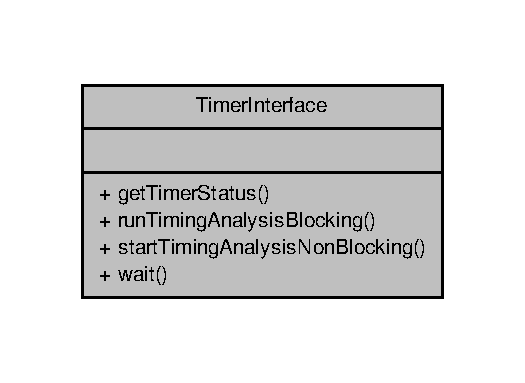
\includegraphics[width=252pt]{classTimerInterface__coll__graph}
\end{center}
\end{figure}
\subsection*{Public Types}
\begin{DoxyCompactItemize}
\item 
enum \hyperlink{classTimerInterface_afc6cca620922cd5a3d90ea9ad7d7d25d}{Status} \{ \\*
\hyperlink{classTimerInterface_afc6cca620922cd5a3d90ea9ad7d7d25da465cc75852c1feab52c2236ed80ef6da}{T\-I\-M\-E\-R\-\_\-\-N\-O\-T\-\_\-\-S\-T\-A\-R\-T\-E\-D} = 0, 
\hyperlink{classTimerInterface_afc6cca620922cd5a3d90ea9ad7d7d25dac7ae064c5a418037be5e05d69a27f34f}{T\-I\-M\-E\-R\-\_\-\-B\-U\-S\-Y}, 
\hyperlink{classTimerInterface_afc6cca620922cd5a3d90ea9ad7d7d25da134d1131be13795c3f8248c82fa52b9e}{T\-I\-M\-E\-R\-\_\-\-F\-I\-N\-I\-S\-H\-E\-D\-\_\-\-S\-U\-C\-C\-E\-S\-S}, 
\hyperlink{classTimerInterface_afc6cca620922cd5a3d90ea9ad7d7d25da5cbb1b932558e1136faa93a49acc0252}{T\-I\-M\-E\-R\-\_\-\-F\-I\-N\-I\-S\-H\-E\-D\-\_\-\-E\-R\-R\-O\-R}, 
\\*
\hyperlink{classTimerInterface_afc6cca620922cd5a3d90ea9ad7d7d25daf5aa3834e4e74e57e8264fdb3b7eb757}{T\-I\-M\-E\-R\-\_\-\-I\-N\-T\-E\-R\-F\-A\-C\-E\-E\-R\-R\-O\-R}
 \}
\end{DoxyCompactItemize}
\subsection*{Static Public Member Functions}
\begin{DoxyCompactItemize}
\item 
static \hyperlink{classTimerInterface_afc6cca620922cd5a3d90ea9ad7d7d25d}{Status} \hyperlink{classTimerInterface_a42077a21e0b9a07b6768e5131415bd2d}{get\-Timer\-Status} (const std\-::string \&contest\-\_\-root, const std\-::string \&benchmark)
\item 
static \hyperlink{classTimerInterface_afc6cca620922cd5a3d90ea9ad7d7d25d}{Status} \hyperlink{classTimerInterface_ada94a843a56747a6a7b34373a266ab92}{run\-Timing\-Analysis\-Blocking} (const std\-::vector$<$ std\-::pair$<$ std\-::string, std\-::string $>$ $>$ \&sizes, const std\-::string \&contest\-\_\-root, const std\-::string \&benchmark, const unsigned polling\-Time)
\item 
static \hyperlink{classTimerInterface_afc6cca620922cd5a3d90ea9ad7d7d25d}{Status} \hyperlink{classTimerInterface_a9a9b69817bbbd603c3d47089b0bad829}{start\-Timing\-Analysis\-Non\-Blocking} (const std\-::vector$<$ std\-::pair$<$ std\-::string, std\-::string $>$ $>$ \&sizes, const std\-::string \&contest\-\_\-root, const std\-::string \&benchmark)
\item 
static void \hyperlink{classTimerInterface_aa62e01d4dd296f8bf9f716ff2da7c5fc}{wait} (int seconds)
\end{DoxyCompactItemize}


\subsection{Detailed Description}
This class contains functions for the timing analysis interface. To use any function belonging to this class, call \hyperlink{classTimerInterface}{Timer\-Interface}\-:\-:$<$function\-\_\-name$>$($<$argument\-\_\-list$>$);. 

Timing Analysis Interface helper class to interface with the timer. This code is provided for description purposes only. The contest organizers cannot guarantee that the provided code is free of bugs or defects. !!!! U\-S\-E T\-H\-I\-S C\-O\-D\-E A\-T Y\-O\-U\-R O\-W\-N R\-I\-S\-K !!!!!

The contestants are free to use these functions as-\/is or make modifications. If the contestants choose to use the provided code, they are responsible for making sure that it works as expected.

The code provided here has no real or implied warranties. 

\subsection{Member Enumeration Documentation}
\hypertarget{classTimerInterface_afc6cca620922cd5a3d90ea9ad7d7d25d}{\index{Timer\-Interface@{Timer\-Interface}!Status@{Status}}
\index{Status@{Status}!TimerInterface@{Timer\-Interface}}
\subsubsection[{Status}]{\setlength{\rightskip}{0pt plus 5cm}enum {\bf Timer\-Interface\-::\-Status}}}\label{classTimerInterface_afc6cca620922cd5a3d90ea9ad7d7d25d}
\begin{Desc}
\item[Enumerator]\par
\begin{description}
\index{T\-I\-M\-E\-R\-\_\-\-N\-O\-T\-\_\-\-S\-T\-A\-R\-T\-E\-D@{T\-I\-M\-E\-R\-\_\-\-N\-O\-T\-\_\-\-S\-T\-A\-R\-T\-E\-D}!Timer\-Interface@{Timer\-Interface}}\index{Timer\-Interface@{Timer\-Interface}!T\-I\-M\-E\-R\-\_\-\-N\-O\-T\-\_\-\-S\-T\-A\-R\-T\-E\-D@{T\-I\-M\-E\-R\-\_\-\-N\-O\-T\-\_\-\-S\-T\-A\-R\-T\-E\-D}}\item[{\em 
\hypertarget{classTimerInterface_afc6cca620922cd5a3d90ea9ad7d7d25da465cc75852c1feab52c2236ed80ef6da}{T\-I\-M\-E\-R\-\_\-\-N\-O\-T\-\_\-\-S\-T\-A\-R\-T\-E\-D}\label{classTimerInterface_afc6cca620922cd5a3d90ea9ad7d7d25da465cc75852c1feab52c2236ed80ef6da}
}]\index{T\-I\-M\-E\-R\-\_\-\-B\-U\-S\-Y@{T\-I\-M\-E\-R\-\_\-\-B\-U\-S\-Y}!Timer\-Interface@{Timer\-Interface}}\index{Timer\-Interface@{Timer\-Interface}!T\-I\-M\-E\-R\-\_\-\-B\-U\-S\-Y@{T\-I\-M\-E\-R\-\_\-\-B\-U\-S\-Y}}\item[{\em 
\hypertarget{classTimerInterface_afc6cca620922cd5a3d90ea9ad7d7d25dac7ae064c5a418037be5e05d69a27f34f}{T\-I\-M\-E\-R\-\_\-\-B\-U\-S\-Y}\label{classTimerInterface_afc6cca620922cd5a3d90ea9ad7d7d25dac7ae064c5a418037be5e05d69a27f34f}
}]\index{T\-I\-M\-E\-R\-\_\-\-F\-I\-N\-I\-S\-H\-E\-D\-\_\-\-S\-U\-C\-C\-E\-S\-S@{T\-I\-M\-E\-R\-\_\-\-F\-I\-N\-I\-S\-H\-E\-D\-\_\-\-S\-U\-C\-C\-E\-S\-S}!Timer\-Interface@{Timer\-Interface}}\index{Timer\-Interface@{Timer\-Interface}!T\-I\-M\-E\-R\-\_\-\-F\-I\-N\-I\-S\-H\-E\-D\-\_\-\-S\-U\-C\-C\-E\-S\-S@{T\-I\-M\-E\-R\-\_\-\-F\-I\-N\-I\-S\-H\-E\-D\-\_\-\-S\-U\-C\-C\-E\-S\-S}}\item[{\em 
\hypertarget{classTimerInterface_afc6cca620922cd5a3d90ea9ad7d7d25da134d1131be13795c3f8248c82fa52b9e}{T\-I\-M\-E\-R\-\_\-\-F\-I\-N\-I\-S\-H\-E\-D\-\_\-\-S\-U\-C\-C\-E\-S\-S}\label{classTimerInterface_afc6cca620922cd5a3d90ea9ad7d7d25da134d1131be13795c3f8248c82fa52b9e}
}]\index{T\-I\-M\-E\-R\-\_\-\-F\-I\-N\-I\-S\-H\-E\-D\-\_\-\-E\-R\-R\-O\-R@{T\-I\-M\-E\-R\-\_\-\-F\-I\-N\-I\-S\-H\-E\-D\-\_\-\-E\-R\-R\-O\-R}!Timer\-Interface@{Timer\-Interface}}\index{Timer\-Interface@{Timer\-Interface}!T\-I\-M\-E\-R\-\_\-\-F\-I\-N\-I\-S\-H\-E\-D\-\_\-\-E\-R\-R\-O\-R@{T\-I\-M\-E\-R\-\_\-\-F\-I\-N\-I\-S\-H\-E\-D\-\_\-\-E\-R\-R\-O\-R}}\item[{\em 
\hypertarget{classTimerInterface_afc6cca620922cd5a3d90ea9ad7d7d25da5cbb1b932558e1136faa93a49acc0252}{T\-I\-M\-E\-R\-\_\-\-F\-I\-N\-I\-S\-H\-E\-D\-\_\-\-E\-R\-R\-O\-R}\label{classTimerInterface_afc6cca620922cd5a3d90ea9ad7d7d25da5cbb1b932558e1136faa93a49acc0252}
}]\index{T\-I\-M\-E\-R\-\_\-\-I\-N\-T\-E\-R\-F\-A\-C\-E\-E\-R\-R\-O\-R@{T\-I\-M\-E\-R\-\_\-\-I\-N\-T\-E\-R\-F\-A\-C\-E\-E\-R\-R\-O\-R}!Timer\-Interface@{Timer\-Interface}}\index{Timer\-Interface@{Timer\-Interface}!T\-I\-M\-E\-R\-\_\-\-I\-N\-T\-E\-R\-F\-A\-C\-E\-E\-R\-R\-O\-R@{T\-I\-M\-E\-R\-\_\-\-I\-N\-T\-E\-R\-F\-A\-C\-E\-E\-R\-R\-O\-R}}\item[{\em 
\hypertarget{classTimerInterface_afc6cca620922cd5a3d90ea9ad7d7d25daf5aa3834e4e74e57e8264fdb3b7eb757}{T\-I\-M\-E\-R\-\_\-\-I\-N\-T\-E\-R\-F\-A\-C\-E\-E\-R\-R\-O\-R}\label{classTimerInterface_afc6cca620922cd5a3d90ea9ad7d7d25daf5aa3834e4e74e57e8264fdb3b7eb757}
}]\end{description}
\end{Desc}


\subsection{Member Function Documentation}
\hypertarget{classTimerInterface_a42077a21e0b9a07b6768e5131415bd2d}{\index{Timer\-Interface@{Timer\-Interface}!get\-Timer\-Status@{get\-Timer\-Status}}
\index{get\-Timer\-Status@{get\-Timer\-Status}!TimerInterface@{Timer\-Interface}}
\subsubsection[{get\-Timer\-Status}]{\setlength{\rightskip}{0pt plus 5cm}static {\bf Status} Timer\-Interface\-::get\-Timer\-Status (
\begin{DoxyParamCaption}
\item[{const std\-::string \&}]{contest\-\_\-root, }
\item[{const std\-::string \&}]{benchmark}
\end{DoxyParamCaption}
)\hspace{0.3cm}{\ttfamily [static]}}}\label{classTimerInterface_a42077a21e0b9a07b6768e5131415bd2d}
Get timer status Inputs\-: contest root directory (string) benchmark name (string) Return\-: status (see enum Status above) \hypertarget{classTimerInterface_ada94a843a56747a6a7b34373a266ab92}{\index{Timer\-Interface@{Timer\-Interface}!run\-Timing\-Analysis\-Blocking@{run\-Timing\-Analysis\-Blocking}}
\index{run\-Timing\-Analysis\-Blocking@{run\-Timing\-Analysis\-Blocking}!TimerInterface@{Timer\-Interface}}
\subsubsection[{run\-Timing\-Analysis\-Blocking}]{\setlength{\rightskip}{0pt plus 5cm}static {\bf Status} Timer\-Interface\-::run\-Timing\-Analysis\-Blocking (
\begin{DoxyParamCaption}
\item[{const std\-::vector$<$ std\-::pair$<$ std\-::string, std\-::string $>$ $>$ \&}]{sizes, }
\item[{const std\-::string \&}]{contest\-\_\-root, }
\item[{const std\-::string \&}]{benchmark, }
\item[{const unsigned}]{polling\-Time}
\end{DoxyParamCaption}
)\hspace{0.3cm}{\ttfamily [static]}}}\label{classTimerInterface_ada94a843a56747a6a7b34373a266ab92}
Write sizes and run timing analysis in blocking mode
\begin{DoxyEnumerate}
\item Write sizes
\item Starts timing analysis
\item Waits for timing analysis to be completed Inputs\-: vector of pairs where first value is instance name (string) and second value is cell name (string) contest root directory (string) benchmark name (string) polling time (number of seconds that the function should wait before polling timer status to check whether timer is done) Return\-: timer status 
\end{DoxyEnumerate}\hypertarget{classTimerInterface_a9a9b69817bbbd603c3d47089b0bad829}{\index{Timer\-Interface@{Timer\-Interface}!start\-Timing\-Analysis\-Non\-Blocking@{start\-Timing\-Analysis\-Non\-Blocking}}
\index{start\-Timing\-Analysis\-Non\-Blocking@{start\-Timing\-Analysis\-Non\-Blocking}!TimerInterface@{Timer\-Interface}}
\subsubsection[{start\-Timing\-Analysis\-Non\-Blocking}]{\setlength{\rightskip}{0pt plus 5cm}static {\bf Status} Timer\-Interface\-::start\-Timing\-Analysis\-Non\-Blocking (
\begin{DoxyParamCaption}
\item[{const std\-::vector$<$ std\-::pair$<$ std\-::string, std\-::string $>$ $>$ \&}]{sizes, }
\item[{const std\-::string \&}]{contest\-\_\-root, }
\item[{const std\-::string \&}]{benchmark}
\end{DoxyParamCaption}
)\hspace{0.3cm}{\ttfamily [static]}}}\label{classTimerInterface_a9a9b69817bbbd603c3d47089b0bad829}
Start timing analysis in non-\/blocking mode
\begin{DoxyEnumerate}
\item Write sizes
\item Starts timing analysis and returns (does not wait for timing analysis to be completed) Inputs\-: vector of pairs where first value is instance name (string) and second value is cell name (string) contest root directory (string) benchmark name (string) Return\-: timer status 
\end{DoxyEnumerate}\hypertarget{classTimerInterface_aa62e01d4dd296f8bf9f716ff2da7c5fc}{\index{Timer\-Interface@{Timer\-Interface}!wait@{wait}}
\index{wait@{wait}!TimerInterface@{Timer\-Interface}}
\subsubsection[{wait}]{\setlength{\rightskip}{0pt plus 5cm}static void Timer\-Interface\-::wait (
\begin{DoxyParamCaption}
\item[{int}]{seconds}
\end{DoxyParamCaption}
)\hspace{0.3cm}{\ttfamily [static]}}}\label{classTimerInterface_aa62e01d4dd296f8bf9f716ff2da7c5fc}
Wait for given number of seconds (useful function if you want to wait before checking timer status after calling start\-Timing\-Analysis\-Non\-Blocking) Input\-: seconds to wait 

The documentation for this class was generated from the following file\-:\begin{DoxyCompactItemize}
\item 
Timing\-Analysis/src/include/\hyperlink{timer__interface_8h}{timer\-\_\-interface.\-h}\end{DoxyCompactItemize}

\hypertarget{classTiming__Analysis_1_1Timing__Analysis}{\section{Timing\-\_\-\-Analysis\-:\-:Timing\-\_\-\-Analysis Class Reference}
\label{classTiming__Analysis_1_1Timing__Analysis}\index{Timing\-\_\-\-Analysis\-::\-Timing\-\_\-\-Analysis@{Timing\-\_\-\-Analysis\-::\-Timing\-\_\-\-Analysis}}
}
\subsection*{Public Member Functions}
\begin{DoxyCompactItemize}
\item 
\hypertarget{classTiming__Analysis_1_1Timing__Analysis_aea46c3c9e4015f3b6802eca8a9c6d798}{{\bfseries Timing\-\_\-\-Analysis} (const \hyperlink{classCircuit__Netlist}{Circuit\-\_\-\-Netlist} \&netlist, const \hyperlink{classLibertyLibrary}{Liberty\-Library} $\ast$lib, const Parasitics $\ast$\-\_\-parasitics, const \hyperlink{classDesign__Constraints}{Design\-\_\-\-Constraints} $\ast$sdc)}\label{classTiming__Analysis_1_1Timing__Analysis_aea46c3c9e4015f3b6802eca8a9c6d798}

\item 
\hypertarget{classTiming__Analysis_1_1Timing__Analysis_ae98e3de81890f6e7b23b58af151e17ab}{void {\bfseries call\-\_\-prime\-\_\-time} ()}\label{classTiming__Analysis_1_1Timing__Analysis_ae98e3de81890f6e7b23b58af151e17ab}

\item 
\hypertarget{classTiming__Analysis_1_1Timing__Analysis_a16566352c5a2b9da08b2c65fadd774de}{void {\bfseries full\-\_\-timing\-\_\-analysis} ()}\label{classTiming__Analysis_1_1Timing__Analysis_a16566352c5a2b9da08b2c65fadd774de}

\item 
\hypertarget{classTiming__Analysis_1_1Timing__Analysis_accd0fc851f665860214942e93242585b}{size\-\_\-t {\bfseries timing\-\_\-points\-\_\-size} ()}\label{classTiming__Analysis_1_1Timing__Analysis_accd0fc851f665860214942e93242585b}

\item 
\hypertarget{classTiming__Analysis_1_1Timing__Analysis_a15ebc83dc364a1e6ec06723658059377}{const \hyperlink{classTiming__Analysis_1_1Timing__Point}{Timing\-\_\-\-Point} \& {\bfseries timing\-\_\-point} (const int i)}\label{classTiming__Analysis_1_1Timing__Analysis_a15ebc83dc364a1e6ec06723658059377}

\item 
\hypertarget{classTiming__Analysis_1_1Timing__Analysis_a239195867157ea06264afcdc3bb54e53}{size\-\_\-t {\bfseries timing\-\_\-arcs\-\_\-size} ()}\label{classTiming__Analysis_1_1Timing__Analysis_a239195867157ea06264afcdc3bb54e53}

\item 
\hypertarget{classTiming__Analysis_1_1Timing__Analysis_ab51fd160e68b13a059efdcc460da1e83}{const \hyperlink{classTiming__Analysis_1_1Timing__Arc}{Timing\-\_\-\-Arc} \& {\bfseries timing\-\_\-arc} (const int i)}\label{classTiming__Analysis_1_1Timing__Analysis_ab51fd160e68b13a059efdcc460da1e83}

\item 
\hypertarget{classTiming__Analysis_1_1Timing__Analysis_a0d0a28110de2017c754373f7a73c160d}{size\-\_\-t {\bfseries timing\-\_\-nets\-\_\-size} ()}\label{classTiming__Analysis_1_1Timing__Analysis_a0d0a28110de2017c754373f7a73c160d}

\item 
\hypertarget{classTiming__Analysis_1_1Timing__Analysis_ab113f7930936110307c215a90e410769}{const \hyperlink{classTiming__Analysis_1_1Timing__Net}{Timing\-\_\-\-Net} \& {\bfseries timing\-\_\-net} (const int i)}\label{classTiming__Analysis_1_1Timing__Analysis_ab113f7930936110307c215a90e410769}

\item 
\hypertarget{classTiming__Analysis_1_1Timing__Analysis_a0263a18b53ef152589a3396423490f78}{double {\bfseries pin\-\_\-capacitance} (const int timing\-\_\-point\-\_\-index) const }\label{classTiming__Analysis_1_1Timing__Analysis_a0263a18b53ef152589a3396423490f78}

\item 
\hypertarget{classTiming__Analysis_1_1Timing__Analysis_a6569529b1614d4507d48293c7ea9f544}{double {\bfseries pin\-\_\-load} (const int timing\-\_\-point\-\_\-index) const }\label{classTiming__Analysis_1_1Timing__Analysis_a6569529b1614d4507d48293c7ea9f544}

\item 
\hypertarget{classTiming__Analysis_1_1Timing__Analysis_a578a7940a493f7e6ab5ca4518984b8d4}{int {\bfseries option} (const int gate\-\_\-number)}\label{classTiming__Analysis_1_1Timing__Analysis_a578a7940a493f7e6ab5ca4518984b8d4}

\item 
\hypertarget{classTiming__Analysis_1_1Timing__Analysis_ad5d0274622ee3f7d2c2f3d731b35ac9a}{bool {\bfseries option} (const int gate\-\_\-index, const int option)}\label{classTiming__Analysis_1_1Timing__Analysis_ad5d0274622ee3f7d2c2f3d731b35ac9a}

\item 
\hypertarget{classTiming__Analysis_1_1Timing__Analysis_aa4220574cd239b38b7905636a6a4e43b}{bool {\bfseries validate\-\_\-with\-\_\-prime\-\_\-time} ()}\label{classTiming__Analysis_1_1Timing__Analysis_aa4220574cd239b38b7905636a6a4e43b}

\item 
\hypertarget{classTiming__Analysis_1_1Timing__Analysis_ad88fd0b79ae6d221a5691da10b0aa9e4}{void {\bfseries print\-\_\-info} ()}\label{classTiming__Analysis_1_1Timing__Analysis_ad88fd0b79ae6d221a5691da10b0aa9e4}

\item 
\hypertarget{classTiming__Analysis_1_1Timing__Analysis_a2c45b5a9fd71b7197a327593d54663a3}{void {\bfseries print\-\_\-circuit\-\_\-info} ()}\label{classTiming__Analysis_1_1Timing__Analysis_a2c45b5a9fd71b7197a327593d54663a3}

\item 
\hypertarget{classTiming__Analysis_1_1Timing__Analysis_a6d3fd296c18a72b05d36addc14068e16}{void {\bfseries report\-\_\-timing} ()}\label{classTiming__Analysis_1_1Timing__Analysis_a6d3fd296c18a72b05d36addc14068e16}

\end{DoxyCompactItemize}


The documentation for this class was generated from the following file\-:\begin{DoxyCompactItemize}
\item 
tcc\-Chrystian/src/include/timing\-\_\-analysis.\-h\end{DoxyCompactItemize}

\hypertarget{classTiming__Analysis_1_1Timing__Arc}{\section{Timing\-\_\-\-Analysis\-:\-:Timing\-\_\-\-Arc Class Reference}
\label{classTiming__Analysis_1_1Timing__Arc}\index{Timing\-\_\-\-Analysis\-::\-Timing\-\_\-\-Arc@{Timing\-\_\-\-Analysis\-::\-Timing\-\_\-\-Arc}}
}


Describes a \hyperlink{classTiming__Analysis_1_1Timing__Arc}{Timing\-\_\-\-Arc} of the timing graph model. Vertex which connects one \hyperlink{classTiming__Analysis_1_1Timing__Point}{Timing\-\_\-\-Point} to another timing point only.  




{\ttfamily \#include $<$timing\-\_\-arc.\-h$>$}



Inheritance diagram for Timing\-\_\-\-Analysis\-:\-:Timing\-\_\-\-Arc\-:\nopagebreak
\begin{figure}[H]
\begin{center}
\leavevmode
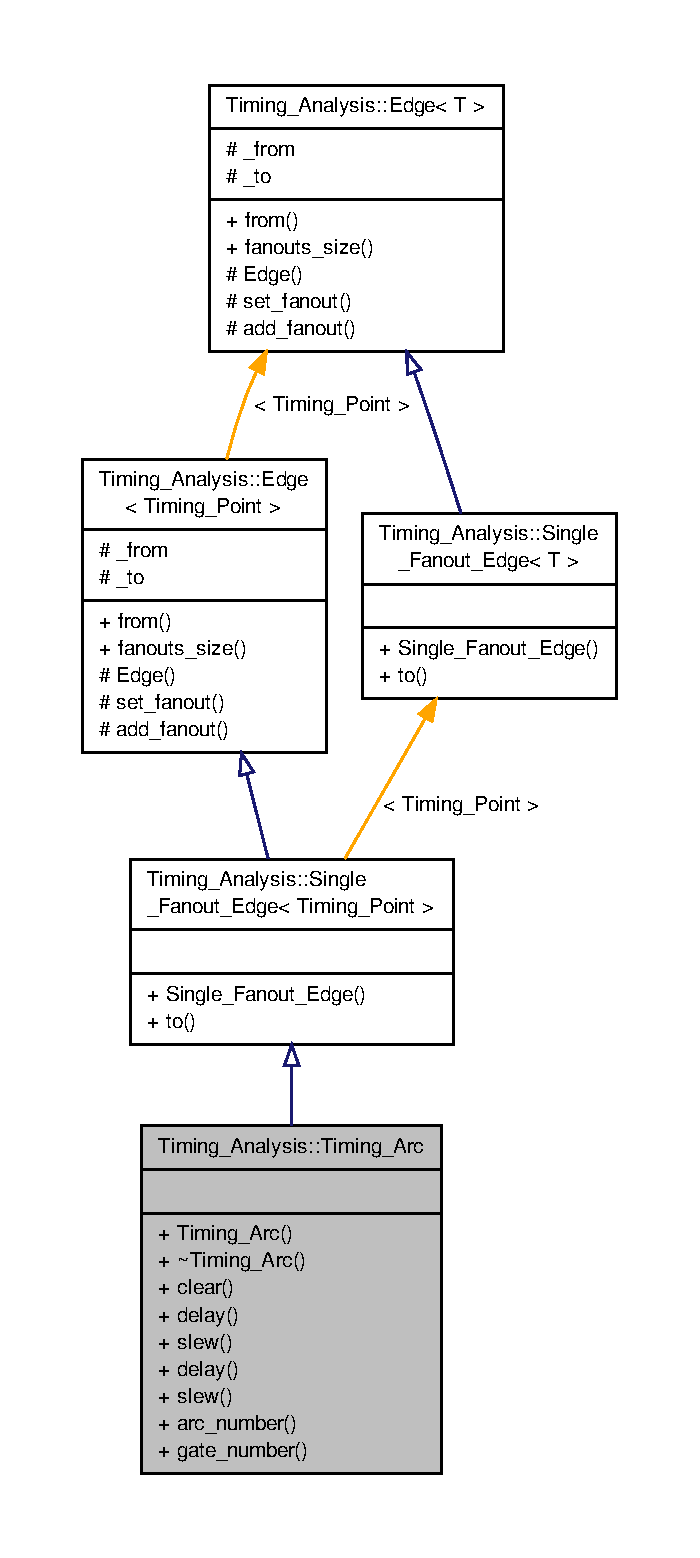
\includegraphics[height=550pt]{classTiming__Analysis_1_1Timing__Arc__inherit__graph}
\end{center}
\end{figure}


Collaboration diagram for Timing\-\_\-\-Analysis\-:\-:Timing\-\_\-\-Arc\-:\nopagebreak
\begin{figure}[H]
\begin{center}
\leavevmode
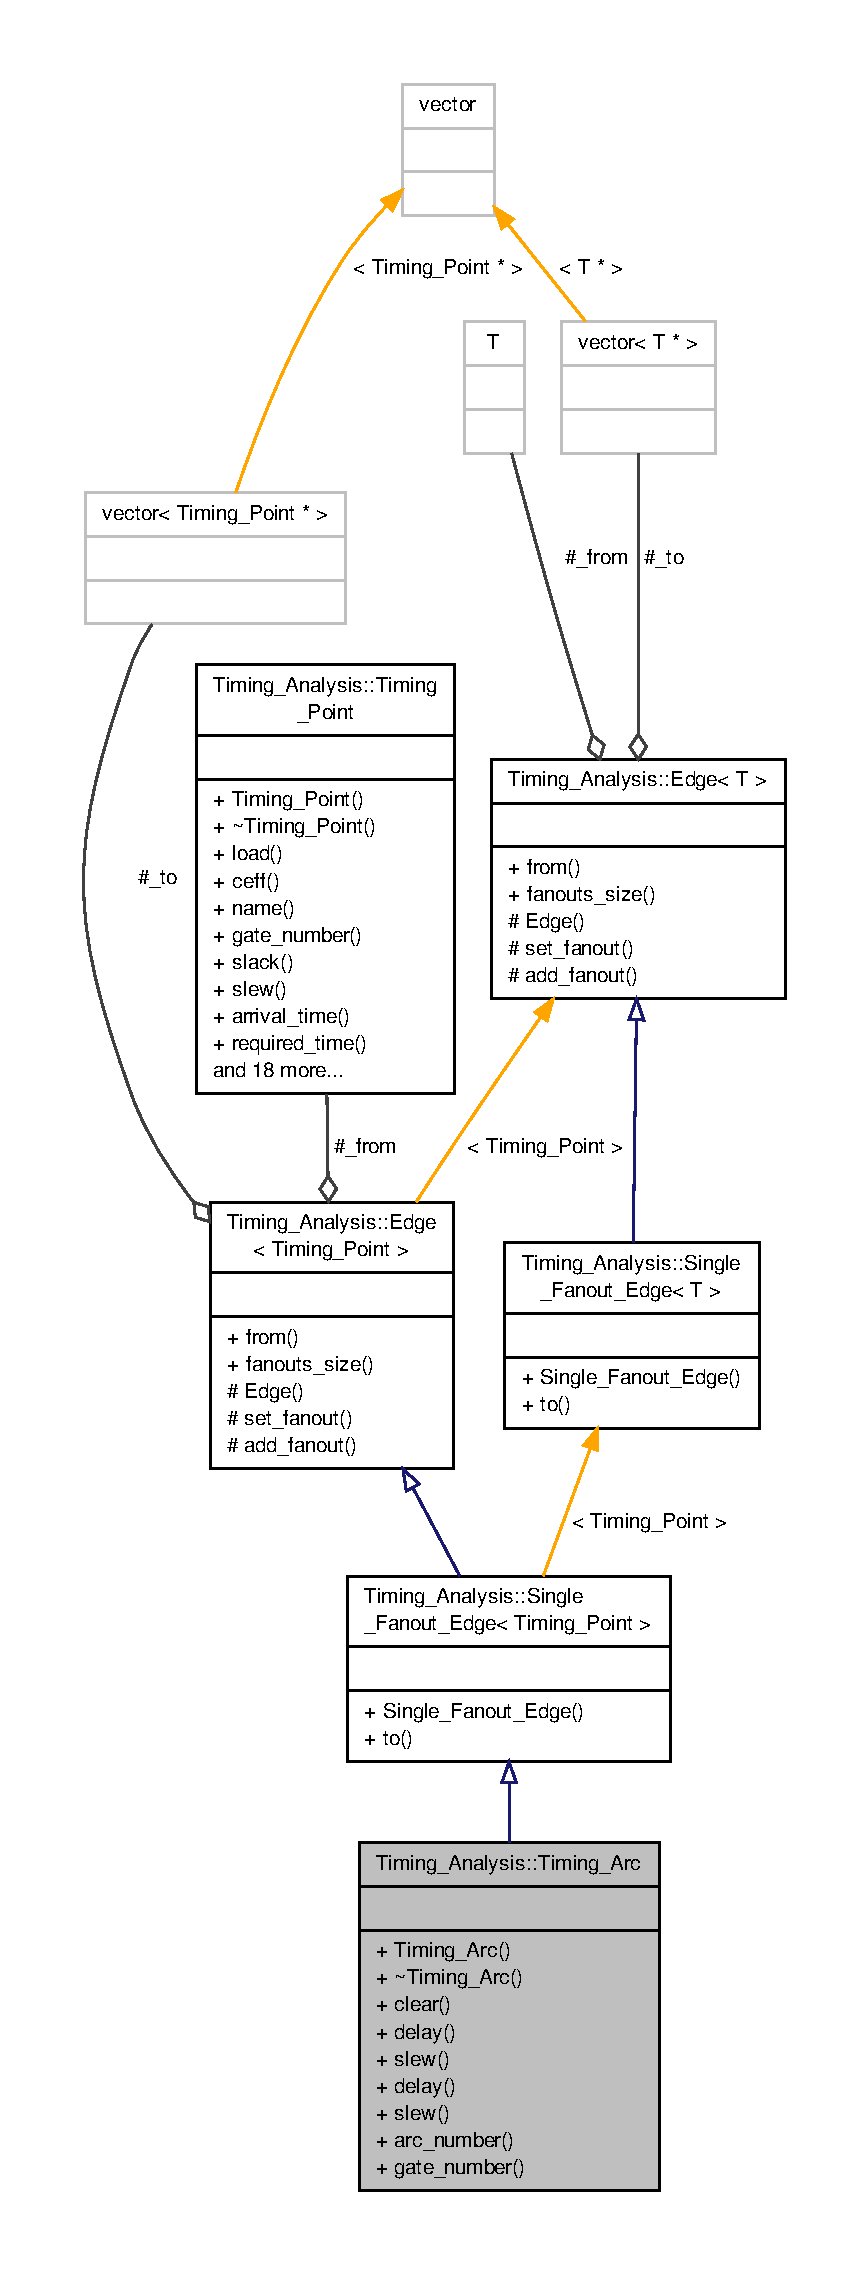
\includegraphics[height=550pt]{classTiming__Analysis_1_1Timing__Arc__coll__graph}
\end{center}
\end{figure}
\subsection*{Public Member Functions}
\begin{DoxyCompactItemize}
\item 
\hyperlink{classTiming__Analysis_1_1Timing__Arc_a38312efc7070c651743a667568514162}{Timing\-\_\-\-Arc} (\hyperlink{classTiming__Analysis_1_1Timing__Point}{Timing\-\_\-\-Point} $\ast$\hyperlink{classTiming__Analysis_1_1Edge_a47020ea89fd9fde438adc814a731a23d}{from}, \hyperlink{classTiming__Analysis_1_1Timing__Point}{Timing\-\_\-\-Point} $\ast$\hyperlink{classTiming__Analysis_1_1Single__Fanout__Edge_ac01deccce158b6cee6883924e6dcb788}{to}, const int arc\-Number, const int \hyperlink{classTiming__Analysis_1_1Timing__Arc_abd085ce8fe10d00d6e0be2668773b32f}{gate\-\_\-number})
\begin{DoxyCompactList}\small\item\em \hyperlink{classTiming__Analysis_1_1Timing__Arc}{Timing\-\_\-\-Arc} constructor. \end{DoxyCompactList}\item 
virtual \hyperlink{classTiming__Analysis_1_1Timing__Arc_a32909fb0fdc3bd5f2a13cdb9f9b351b8}{$\sim$\-Timing\-\_\-\-Arc} ()
\begin{DoxyCompactList}\small\item\em \hyperlink{classTiming__Analysis_1_1Timing__Arc}{Timing\-\_\-\-Arc} destructor. \end{DoxyCompactList}\item 
void \hyperlink{classTiming__Analysis_1_1Timing__Arc_a092de659dd0846a3e899f0efd9c34397}{clear} ()
\begin{DoxyCompactList}\small\item\em Sets delay and slew time to zero. \end{DoxyCompactList}\item 
\hyperlink{classTransitions}{Transitions}$<$ double $>$ \hyperlink{classTiming__Analysis_1_1Timing__Arc_a6561e6eb77cc7536f5515db318b233ce}{delay} () const 
\begin{DoxyCompactList}\small\item\em Returns delay time. \end{DoxyCompactList}\item 
\hyperlink{classTransitions}{Transitions}$<$ double $>$ \hyperlink{classTiming__Analysis_1_1Timing__Arc_a9846eb6bd9afc2cd8cbb0f926daf39a5}{slew} () const 
\begin{DoxyCompactList}\small\item\em Returns slew time. \end{DoxyCompactList}\item 
void \hyperlink{classTiming__Analysis_1_1Timing__Arc_a74682f1b90b14cb0902dca32e6430fd2}{delay} (const \hyperlink{classTransitions}{Transitions}$<$ double $>$ \&delay)
\begin{DoxyCompactList}\small\item\em Sets delay time. \end{DoxyCompactList}\item 
void \hyperlink{classTiming__Analysis_1_1Timing__Arc_a5521ea0890331cb77e6b0ea72a7062a3}{slew} (const \hyperlink{classTransitions}{Transitions}$<$ double $>$ \&slew)
\begin{DoxyCompactList}\small\item\em Sets slew time. \end{DoxyCompactList}\item 
int \hyperlink{classTiming__Analysis_1_1Timing__Arc_aa4a54ed3cd6762bd26a3fdf566b5a234}{arc\-\_\-number} () const 
\begin{DoxyCompactList}\small\item\em Returns arc number. \end{DoxyCompactList}\item 
int \hyperlink{classTiming__Analysis_1_1Timing__Arc_abd085ce8fe10d00d6e0be2668773b32f}{gate\-\_\-number} () const 
\begin{DoxyCompactList}\small\item\em Returns gate number. \end{DoxyCompactList}\end{DoxyCompactItemize}
\subsection*{Friends}
\begin{DoxyCompactItemize}
\item 
ostream \& \hyperlink{classTiming__Analysis_1_1Timing__Arc_ae33a875fefadb96a5cdf5a17791c4d24}{operator$<$$<$} (ostream \&out, const \hyperlink{classTiming__Analysis_1_1Timing__Arc}{Timing\-\_\-\-Arc} \&ta)
\begin{DoxyCompactList}\small\item\em Inserts formatted description of timing arc, including the origin vertex and destiny vertex. \end{DoxyCompactList}\end{DoxyCompactItemize}
\subsection*{Additional Inherited Members}


\subsection{Detailed Description}
Describes a \hyperlink{classTiming__Analysis_1_1Timing__Arc}{Timing\-\_\-\-Arc} of the timing graph model. Vertex which connects one \hyperlink{classTiming__Analysis_1_1Timing__Point}{Timing\-\_\-\-Point} to another timing point only. 



\subsection{Constructor \& Destructor Documentation}
\hypertarget{classTiming__Analysis_1_1Timing__Arc_a38312efc7070c651743a667568514162}{\index{Timing\-\_\-\-Analysis\-::\-Timing\-\_\-\-Arc@{Timing\-\_\-\-Analysis\-::\-Timing\-\_\-\-Arc}!Timing\-\_\-\-Arc@{Timing\-\_\-\-Arc}}
\index{Timing\-\_\-\-Arc@{Timing\-\_\-\-Arc}!Timing_Analysis::Timing_Arc@{Timing\-\_\-\-Analysis\-::\-Timing\-\_\-\-Arc}}
\subsubsection[{Timing\-\_\-\-Arc}]{\setlength{\rightskip}{0pt plus 5cm}Timing\-\_\-\-Analysis\-::\-Timing\-\_\-\-Arc\-::\-Timing\-\_\-\-Arc (
\begin{DoxyParamCaption}
\item[{{\bf Timing\-\_\-\-Point} $\ast$}]{from, }
\item[{{\bf Timing\-\_\-\-Point} $\ast$}]{to, }
\item[{const int}]{arc\-Number, }
\item[{const int}]{gate\-\_\-number}
\end{DoxyParamCaption}
)\hspace{0.3cm}{\ttfamily [inline]}}}\label{classTiming__Analysis_1_1Timing__Arc_a38312efc7070c651743a667568514162}


\hyperlink{classTiming__Analysis_1_1Timing__Arc}{Timing\-\_\-\-Arc} constructor. 


\begin{DoxyParams}{Parameters}
{\em \hyperlink{classTiming__Analysis_1_1Timing__Point}{Timing\-\_\-\-Point}} & $\ast$ from, \hyperlink{classTiming__Analysis_1_1Timing__Point}{Timing\-\_\-\-Point} $\ast$ to, const int arc\-Number, const int gate\-\_\-number) \-: \hyperlink{classTiming__Analysis_1_1Single__Fanout__Edge}{Single\-\_\-\-Fanout\-\_\-\-Edge$<$\-Timing\-\_\-\-Point$>$(from, to)}, \-\_\-delay(0.\-0f, 0.\-0f), \-\_\-slew(0.\-0f, 0.\-0f), \-\_\-arc\-\_\-number (arc\-Number), \-\_\-gate\-\_\-number(gate\-\_\-number) \\
\hline
\end{DoxyParams}
\hypertarget{classTiming__Analysis_1_1Timing__Arc_a32909fb0fdc3bd5f2a13cdb9f9b351b8}{\index{Timing\-\_\-\-Analysis\-::\-Timing\-\_\-\-Arc@{Timing\-\_\-\-Analysis\-::\-Timing\-\_\-\-Arc}!$\sim$\-Timing\-\_\-\-Arc@{$\sim$\-Timing\-\_\-\-Arc}}
\index{$\sim$\-Timing\-\_\-\-Arc@{$\sim$\-Timing\-\_\-\-Arc}!Timing_Analysis::Timing_Arc@{Timing\-\_\-\-Analysis\-::\-Timing\-\_\-\-Arc}}
\subsubsection[{$\sim$\-Timing\-\_\-\-Arc}]{\setlength{\rightskip}{0pt plus 5cm}virtual Timing\-\_\-\-Analysis\-::\-Timing\-\_\-\-Arc\-::$\sim$\-Timing\-\_\-\-Arc (
\begin{DoxyParamCaption}
{}
\end{DoxyParamCaption}
)\hspace{0.3cm}{\ttfamily [inline]}, {\ttfamily [virtual]}}}\label{classTiming__Analysis_1_1Timing__Arc_a32909fb0fdc3bd5f2a13cdb9f9b351b8}


\hyperlink{classTiming__Analysis_1_1Timing__Arc}{Timing\-\_\-\-Arc} destructor. 



\subsection{Member Function Documentation}
\hypertarget{classTiming__Analysis_1_1Timing__Arc_aa4a54ed3cd6762bd26a3fdf566b5a234}{\index{Timing\-\_\-\-Analysis\-::\-Timing\-\_\-\-Arc@{Timing\-\_\-\-Analysis\-::\-Timing\-\_\-\-Arc}!arc\-\_\-number@{arc\-\_\-number}}
\index{arc\-\_\-number@{arc\-\_\-number}!Timing_Analysis::Timing_Arc@{Timing\-\_\-\-Analysis\-::\-Timing\-\_\-\-Arc}}
\subsubsection[{arc\-\_\-number}]{\setlength{\rightskip}{0pt plus 5cm}int Timing\-\_\-\-Analysis\-::\-Timing\-\_\-\-Arc\-::arc\-\_\-number (
\begin{DoxyParamCaption}
{}
\end{DoxyParamCaption}
) const\hspace{0.3cm}{\ttfamily [inline]}}}\label{classTiming__Analysis_1_1Timing__Arc_aa4a54ed3cd6762bd26a3fdf566b5a234}


Returns arc number. 

\begin{DoxyReturn}{Returns}
int 
\end{DoxyReturn}
\hypertarget{classTiming__Analysis_1_1Timing__Arc_a092de659dd0846a3e899f0efd9c34397}{\index{Timing\-\_\-\-Analysis\-::\-Timing\-\_\-\-Arc@{Timing\-\_\-\-Analysis\-::\-Timing\-\_\-\-Arc}!clear@{clear}}
\index{clear@{clear}!Timing_Analysis::Timing_Arc@{Timing\-\_\-\-Analysis\-::\-Timing\-\_\-\-Arc}}
\subsubsection[{clear}]{\setlength{\rightskip}{0pt plus 5cm}void Timing\-\_\-\-Analysis\-::\-Timing\-\_\-\-Arc\-::clear (
\begin{DoxyParamCaption}
{}
\end{DoxyParamCaption}
)}}\label{classTiming__Analysis_1_1Timing__Arc_a092de659dd0846a3e899f0efd9c34397}


Sets delay and slew time to zero. 

\begin{DoxyReturn}{Returns}
void 
\end{DoxyReturn}
\hypertarget{classTiming__Analysis_1_1Timing__Arc_a6561e6eb77cc7536f5515db318b233ce}{\index{Timing\-\_\-\-Analysis\-::\-Timing\-\_\-\-Arc@{Timing\-\_\-\-Analysis\-::\-Timing\-\_\-\-Arc}!delay@{delay}}
\index{delay@{delay}!Timing_Analysis::Timing_Arc@{Timing\-\_\-\-Analysis\-::\-Timing\-\_\-\-Arc}}
\subsubsection[{delay}]{\setlength{\rightskip}{0pt plus 5cm}{\bf Transitions}$<$double$>$ Timing\-\_\-\-Analysis\-::\-Timing\-\_\-\-Arc\-::delay (
\begin{DoxyParamCaption}
{}
\end{DoxyParamCaption}
) const\hspace{0.3cm}{\ttfamily [inline]}}}\label{classTiming__Analysis_1_1Timing__Arc_a6561e6eb77cc7536f5515db318b233ce}


Returns delay time. 

\begin{DoxyReturn}{Returns}
\hyperlink{classTransitions}{Transitions$<$double$>$} 
\end{DoxyReturn}
\hypertarget{classTiming__Analysis_1_1Timing__Arc_a74682f1b90b14cb0902dca32e6430fd2}{\index{Timing\-\_\-\-Analysis\-::\-Timing\-\_\-\-Arc@{Timing\-\_\-\-Analysis\-::\-Timing\-\_\-\-Arc}!delay@{delay}}
\index{delay@{delay}!Timing_Analysis::Timing_Arc@{Timing\-\_\-\-Analysis\-::\-Timing\-\_\-\-Arc}}
\subsubsection[{delay}]{\setlength{\rightskip}{0pt plus 5cm}void Timing\-\_\-\-Analysis\-::\-Timing\-\_\-\-Arc\-::delay (
\begin{DoxyParamCaption}
\item[{const {\bf Transitions}$<$ double $>$ \&}]{delay}
\end{DoxyParamCaption}
)\hspace{0.3cm}{\ttfamily [inline]}}}\label{classTiming__Analysis_1_1Timing__Arc_a74682f1b90b14cb0902dca32e6430fd2}


Sets delay time. 

\begin{DoxyReturn}{Returns}
void 
\end{DoxyReturn}


Here is the call graph for this function\-:\nopagebreak
\begin{figure}[H]
\begin{center}
\leavevmode
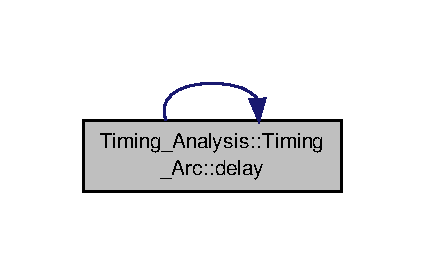
\includegraphics[width=204pt]{classTiming__Analysis_1_1Timing__Arc_a74682f1b90b14cb0902dca32e6430fd2_cgraph}
\end{center}
\end{figure}




Here is the caller graph for this function\-:\nopagebreak
\begin{figure}[H]
\begin{center}
\leavevmode
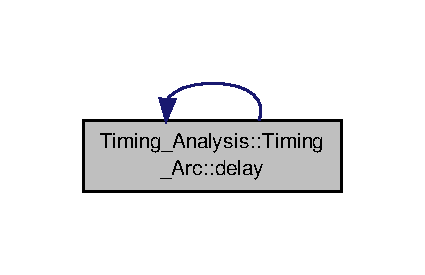
\includegraphics[width=204pt]{classTiming__Analysis_1_1Timing__Arc_a74682f1b90b14cb0902dca32e6430fd2_icgraph}
\end{center}
\end{figure}


\hypertarget{classTiming__Analysis_1_1Timing__Arc_abd085ce8fe10d00d6e0be2668773b32f}{\index{Timing\-\_\-\-Analysis\-::\-Timing\-\_\-\-Arc@{Timing\-\_\-\-Analysis\-::\-Timing\-\_\-\-Arc}!gate\-\_\-number@{gate\-\_\-number}}
\index{gate\-\_\-number@{gate\-\_\-number}!Timing_Analysis::Timing_Arc@{Timing\-\_\-\-Analysis\-::\-Timing\-\_\-\-Arc}}
\subsubsection[{gate\-\_\-number}]{\setlength{\rightskip}{0pt plus 5cm}int Timing\-\_\-\-Analysis\-::\-Timing\-\_\-\-Arc\-::gate\-\_\-number (
\begin{DoxyParamCaption}
{}
\end{DoxyParamCaption}
) const\hspace{0.3cm}{\ttfamily [inline]}}}\label{classTiming__Analysis_1_1Timing__Arc_abd085ce8fe10d00d6e0be2668773b32f}


Returns gate number. 

\begin{DoxyReturn}{Returns}
void 
\end{DoxyReturn}
\hypertarget{classTiming__Analysis_1_1Timing__Arc_a9846eb6bd9afc2cd8cbb0f926daf39a5}{\index{Timing\-\_\-\-Analysis\-::\-Timing\-\_\-\-Arc@{Timing\-\_\-\-Analysis\-::\-Timing\-\_\-\-Arc}!slew@{slew}}
\index{slew@{slew}!Timing_Analysis::Timing_Arc@{Timing\-\_\-\-Analysis\-::\-Timing\-\_\-\-Arc}}
\subsubsection[{slew}]{\setlength{\rightskip}{0pt plus 5cm}{\bf Transitions}$<$double$>$ Timing\-\_\-\-Analysis\-::\-Timing\-\_\-\-Arc\-::slew (
\begin{DoxyParamCaption}
{}
\end{DoxyParamCaption}
) const\hspace{0.3cm}{\ttfamily [inline]}}}\label{classTiming__Analysis_1_1Timing__Arc_a9846eb6bd9afc2cd8cbb0f926daf39a5}


Returns slew time. 

\begin{DoxyReturn}{Returns}
\hyperlink{classTransitions}{Transitions$<$double$>$} 
\end{DoxyReturn}
\hypertarget{classTiming__Analysis_1_1Timing__Arc_a5521ea0890331cb77e6b0ea72a7062a3}{\index{Timing\-\_\-\-Analysis\-::\-Timing\-\_\-\-Arc@{Timing\-\_\-\-Analysis\-::\-Timing\-\_\-\-Arc}!slew@{slew}}
\index{slew@{slew}!Timing_Analysis::Timing_Arc@{Timing\-\_\-\-Analysis\-::\-Timing\-\_\-\-Arc}}
\subsubsection[{slew}]{\setlength{\rightskip}{0pt plus 5cm}void Timing\-\_\-\-Analysis\-::\-Timing\-\_\-\-Arc\-::slew (
\begin{DoxyParamCaption}
\item[{const {\bf Transitions}$<$ double $>$ \&}]{slew}
\end{DoxyParamCaption}
)\hspace{0.3cm}{\ttfamily [inline]}}}\label{classTiming__Analysis_1_1Timing__Arc_a5521ea0890331cb77e6b0ea72a7062a3}


Sets slew time. 

\begin{DoxyReturn}{Returns}
void 
\end{DoxyReturn}


Here is the call graph for this function\-:\nopagebreak
\begin{figure}[H]
\begin{center}
\leavevmode
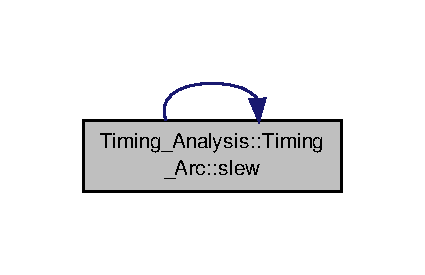
\includegraphics[width=204pt]{classTiming__Analysis_1_1Timing__Arc_a5521ea0890331cb77e6b0ea72a7062a3_cgraph}
\end{center}
\end{figure}




Here is the caller graph for this function\-:\nopagebreak
\begin{figure}[H]
\begin{center}
\leavevmode
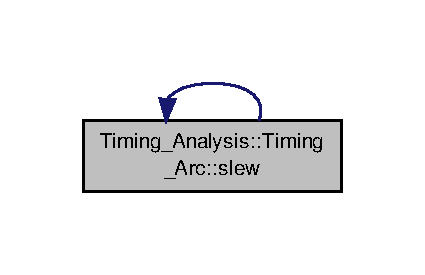
\includegraphics[width=204pt]{classTiming__Analysis_1_1Timing__Arc_a5521ea0890331cb77e6b0ea72a7062a3_icgraph}
\end{center}
\end{figure}




\subsection{Friends And Related Function Documentation}
\hypertarget{classTiming__Analysis_1_1Timing__Arc_ae33a875fefadb96a5cdf5a17791c4d24}{\index{Timing\-\_\-\-Analysis\-::\-Timing\-\_\-\-Arc@{Timing\-\_\-\-Analysis\-::\-Timing\-\_\-\-Arc}!operator$<$$<$@{operator$<$$<$}}
\index{operator$<$$<$@{operator$<$$<$}!Timing_Analysis::Timing_Arc@{Timing\-\_\-\-Analysis\-::\-Timing\-\_\-\-Arc}}
\subsubsection[{operator$<$$<$}]{\setlength{\rightskip}{0pt plus 5cm}ostream\& operator$<$$<$ (
\begin{DoxyParamCaption}
\item[{ostream \&}]{out, }
\item[{const {\bf Timing\-\_\-\-Arc} \&}]{ta}
\end{DoxyParamCaption}
)\hspace{0.3cm}{\ttfamily [friend]}}}\label{classTiming__Analysis_1_1Timing__Arc_ae33a875fefadb96a5cdf5a17791c4d24}


Inserts formatted description of timing arc, including the origin vertex and destiny vertex. 



The documentation for this class was generated from the following file\-:\begin{DoxyCompactItemize}
\item 
Timing\-Analysis/src/include/\hyperlink{timing__arc_8h}{timing\-\_\-arc.\-h}\end{DoxyCompactItemize}

\hypertarget{classTiming__Analysis_1_1Timing__Net}{\section{Timing\-\_\-\-Analysis\-:\-:Timing\-\_\-\-Net Class Reference}
\label{classTiming__Analysis_1_1Timing__Net}\index{Timing\-\_\-\-Analysis\-::\-Timing\-\_\-\-Net@{Timing\-\_\-\-Analysis\-::\-Timing\-\_\-\-Net}}
}


Describes a timing net of the timing graph model.  




{\ttfamily \#include $<$timing\-\_\-net.\-h$>$}

Inheritance diagram for Timing\-\_\-\-Analysis\-:\-:Timing\-\_\-\-Net\-:\begin{figure}[H]
\begin{center}
\leavevmode
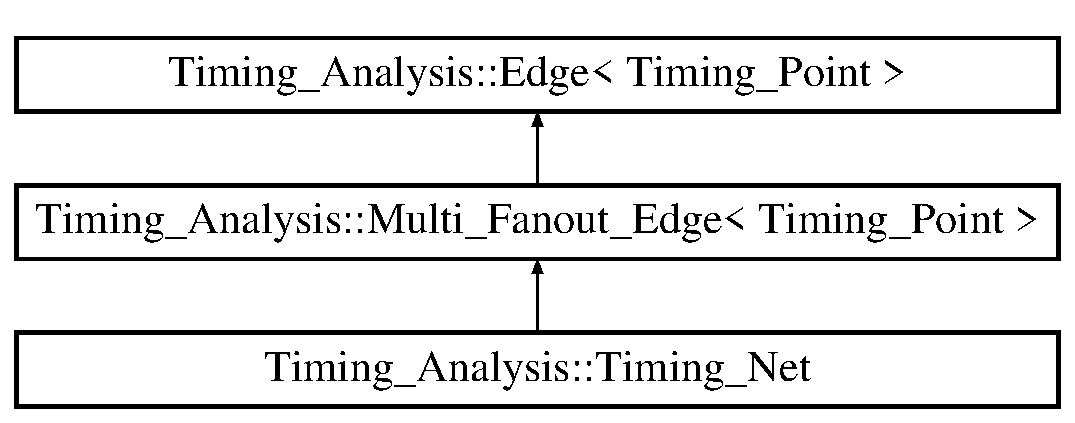
\includegraphics[height=3.000000cm]{classTiming__Analysis_1_1Timing__Net}
\end{center}
\end{figure}
\subsection*{Public Member Functions}
\begin{DoxyCompactItemize}
\item 
\hyperlink{classTiming__Analysis_1_1Timing__Net_aa31562b888cce5b1ad2a4198ad6c37d1}{Timing\-\_\-\-Net} (const string \&\hyperlink{classTiming__Analysis_1_1Timing__Net_aa21494aaaade42ab7578e697b9fc5d14}{name}, \hyperlink{classTiming__Analysis_1_1Timing__Point}{Timing\-\_\-\-Point} $\ast$\hyperlink{classTiming__Analysis_1_1Edge_a47020ea89fd9fde438adc814a731a23d}{from}, \hyperlink{classWireDelayModel}{Wire\-Delay\-Model} $\ast$\hyperlink{classTiming__Analysis_1_1Timing__Net_ac8cd484d33ccb714f2611a04dd653a66}{wire\-\_\-delay\-\_\-model})
\begin{DoxyCompactList}\small\item\em \hyperlink{classTiming__Analysis_1_1Timing__Net}{Timing\-\_\-\-Net} constructor. \end{DoxyCompactList}\item 
virtual \hyperlink{classTiming__Analysis_1_1Timing__Net_a919bdd9eb5b7d00b1c6b692bb34d6b6b}{$\sim$\-Timing\-\_\-\-Net} ()
\begin{DoxyCompactList}\small\item\em Empty \hyperlink{classTiming__Analysis_1_1Timing__Net}{Timing\-\_\-\-Net} destructor. \end{DoxyCompactList}\item 
const string \hyperlink{classTiming__Analysis_1_1Timing__Net_aa21494aaaade42ab7578e697b9fc5d14}{name} () const 
\begin{DoxyCompactList}\small\item\em Returns \hyperlink{classTiming__Analysis_1_1Timing__Net}{Timing\-\_\-\-Net} name. \end{DoxyCompactList}\item 
\hyperlink{classWireDelayModel}{Wire\-Delay\-Model} $\ast$ \hyperlink{classTiming__Analysis_1_1Timing__Net_ac8cd484d33ccb714f2611a04dd653a66}{wire\-\_\-delay\-\_\-model} ()
\begin{DoxyCompactList}\small\item\em Returns pointer to \hyperlink{classWireDelayModel}{Wire\-Delay\-Model}. \end{DoxyCompactList}\end{DoxyCompactItemize}
\subsection*{Friends}
\begin{DoxyCompactItemize}
\item 
\hypertarget{classTiming__Analysis_1_1Timing__Net_aab560f9cdcd55852a6a08a29a54a2b16}{class {\bfseries Timing\-\_\-\-Analysis}}\label{classTiming__Analysis_1_1Timing__Net_aab560f9cdcd55852a6a08a29a54a2b16}

\item 
\hypertarget{classTiming__Analysis_1_1Timing__Net_a2562d249ea959d9e392abdffe35cdbad}{class {\bfseries Timing\-\_\-\-Point}}\label{classTiming__Analysis_1_1Timing__Net_a2562d249ea959d9e392abdffe35cdbad}

\item 
ostream \& \hyperlink{classTiming__Analysis_1_1Timing__Net_affa1b519dc847065ac579b4c8726c740}{operator$<$$<$} (ostream \&out, const \hyperlink{classTiming__Analysis_1_1Timing__Net}{Timing\-\_\-\-Net} \&tn)
\begin{DoxyCompactList}\small\item\em Redefinition of $<$$<$ operator. Inserts formatted description including \hyperlink{classTiming__Analysis_1_1Timing__Net}{Timing\-\_\-\-Net} name. \end{DoxyCompactList}\end{DoxyCompactItemize}
\subsection*{Additional Inherited Members}


\subsection{Detailed Description}
Describes a timing net of the timing graph model. 



\subsection{Constructor \& Destructor Documentation}
\hypertarget{classTiming__Analysis_1_1Timing__Net_aa31562b888cce5b1ad2a4198ad6c37d1}{\index{Timing\-\_\-\-Analysis\-::\-Timing\-\_\-\-Net@{Timing\-\_\-\-Analysis\-::\-Timing\-\_\-\-Net}!Timing\-\_\-\-Net@{Timing\-\_\-\-Net}}
\index{Timing\-\_\-\-Net@{Timing\-\_\-\-Net}!Timing_Analysis::Timing_Net@{Timing\-\_\-\-Analysis\-::\-Timing\-\_\-\-Net}}
\subsubsection[{Timing\-\_\-\-Net}]{\setlength{\rightskip}{0pt plus 5cm}Timing\-\_\-\-Analysis\-::\-Timing\-\_\-\-Net\-::\-Timing\-\_\-\-Net (
\begin{DoxyParamCaption}
\item[{const string \&}]{name, }
\item[{{\bf Timing\-\_\-\-Point} $\ast$}]{from, }
\item[{{\bf Wire\-Delay\-Model} $\ast$}]{wire\-\_\-delay\-\_\-model}
\end{DoxyParamCaption}
)\hspace{0.3cm}{\ttfamily [inline]}}}\label{classTiming__Analysis_1_1Timing__Net_aa31562b888cce5b1ad2a4198ad6c37d1}


\hyperlink{classTiming__Analysis_1_1Timing__Net}{Timing\-\_\-\-Net} constructor. 


\begin{DoxyParams}{Parameters}
{\em const} & string \& name, \hyperlink{classTiming__Analysis_1_1Timing__Point}{Timing\-\_\-\-Point} $\ast$ from, \hyperlink{classWireDelayModel}{Wire\-Delay\-Model} $\ast$ wire\-\_\-delay\-\_\-model \\
\hline
\end{DoxyParams}
\hypertarget{classTiming__Analysis_1_1Timing__Net_a919bdd9eb5b7d00b1c6b692bb34d6b6b}{\index{Timing\-\_\-\-Analysis\-::\-Timing\-\_\-\-Net@{Timing\-\_\-\-Analysis\-::\-Timing\-\_\-\-Net}!$\sim$\-Timing\-\_\-\-Net@{$\sim$\-Timing\-\_\-\-Net}}
\index{$\sim$\-Timing\-\_\-\-Net@{$\sim$\-Timing\-\_\-\-Net}!Timing_Analysis::Timing_Net@{Timing\-\_\-\-Analysis\-::\-Timing\-\_\-\-Net}}
\subsubsection[{$\sim$\-Timing\-\_\-\-Net}]{\setlength{\rightskip}{0pt plus 5cm}virtual Timing\-\_\-\-Analysis\-::\-Timing\-\_\-\-Net\-::$\sim$\-Timing\-\_\-\-Net (
\begin{DoxyParamCaption}
{}
\end{DoxyParamCaption}
)\hspace{0.3cm}{\ttfamily [inline]}, {\ttfamily [virtual]}}}\label{classTiming__Analysis_1_1Timing__Net_a919bdd9eb5b7d00b1c6b692bb34d6b6b}


Empty \hyperlink{classTiming__Analysis_1_1Timing__Net}{Timing\-\_\-\-Net} destructor. 



\subsection{Member Function Documentation}
\hypertarget{classTiming__Analysis_1_1Timing__Net_aa21494aaaade42ab7578e697b9fc5d14}{\index{Timing\-\_\-\-Analysis\-::\-Timing\-\_\-\-Net@{Timing\-\_\-\-Analysis\-::\-Timing\-\_\-\-Net}!name@{name}}
\index{name@{name}!Timing_Analysis::Timing_Net@{Timing\-\_\-\-Analysis\-::\-Timing\-\_\-\-Net}}
\subsubsection[{name}]{\setlength{\rightskip}{0pt plus 5cm}const string Timing\-\_\-\-Analysis\-::\-Timing\-\_\-\-Net\-::name (
\begin{DoxyParamCaption}
{}
\end{DoxyParamCaption}
) const}}\label{classTiming__Analysis_1_1Timing__Net_aa21494aaaade42ab7578e697b9fc5d14}


Returns \hyperlink{classTiming__Analysis_1_1Timing__Net}{Timing\-\_\-\-Net} name. 

\begin{DoxyReturn}{Returns}
const string 
\end{DoxyReturn}
\hypertarget{classTiming__Analysis_1_1Timing__Net_ac8cd484d33ccb714f2611a04dd653a66}{\index{Timing\-\_\-\-Analysis\-::\-Timing\-\_\-\-Net@{Timing\-\_\-\-Analysis\-::\-Timing\-\_\-\-Net}!wire\-\_\-delay\-\_\-model@{wire\-\_\-delay\-\_\-model}}
\index{wire\-\_\-delay\-\_\-model@{wire\-\_\-delay\-\_\-model}!Timing_Analysis::Timing_Net@{Timing\-\_\-\-Analysis\-::\-Timing\-\_\-\-Net}}
\subsubsection[{wire\-\_\-delay\-\_\-model}]{\setlength{\rightskip}{0pt plus 5cm}{\bf Wire\-Delay\-Model}$\ast$ Timing\-\_\-\-Analysis\-::\-Timing\-\_\-\-Net\-::wire\-\_\-delay\-\_\-model (
\begin{DoxyParamCaption}
{}
\end{DoxyParamCaption}
)\hspace{0.3cm}{\ttfamily [inline]}}}\label{classTiming__Analysis_1_1Timing__Net_ac8cd484d33ccb714f2611a04dd653a66}


Returns pointer to \hyperlink{classWireDelayModel}{Wire\-Delay\-Model}. 

\begin{DoxyReturn}{Returns}
\hyperlink{classWireDelayModel}{Wire\-Delay\-Model} $\ast$ 
\end{DoxyReturn}


\subsection{Friends And Related Function Documentation}
\hypertarget{classTiming__Analysis_1_1Timing__Net_affa1b519dc847065ac579b4c8726c740}{\index{Timing\-\_\-\-Analysis\-::\-Timing\-\_\-\-Net@{Timing\-\_\-\-Analysis\-::\-Timing\-\_\-\-Net}!operator$<$$<$@{operator$<$$<$}}
\index{operator$<$$<$@{operator$<$$<$}!Timing_Analysis::Timing_Net@{Timing\-\_\-\-Analysis\-::\-Timing\-\_\-\-Net}}
\subsubsection[{operator$<$$<$}]{\setlength{\rightskip}{0pt plus 5cm}ostream\& operator$<$$<$ (
\begin{DoxyParamCaption}
\item[{ostream \&}]{out, }
\item[{const {\bf Timing\-\_\-\-Net} \&}]{tn}
\end{DoxyParamCaption}
)\hspace{0.3cm}{\ttfamily [friend]}}}\label{classTiming__Analysis_1_1Timing__Net_affa1b519dc847065ac579b4c8726c740}


Redefinition of $<$$<$ operator. Inserts formatted description including \hyperlink{classTiming__Analysis_1_1Timing__Net}{Timing\-\_\-\-Net} name. 



The documentation for this class was generated from the following file\-:\begin{DoxyCompactItemize}
\item 
tcc\-Chrystian/src/include/timing\-\_\-net.\-h\end{DoxyCompactItemize}

\hypertarget{classTiming__Analysis_1_1Timing__Point}{\section{Timing\-\_\-\-Analysis\-:\-:Timing\-\_\-\-Point Class Reference}
\label{classTiming__Analysis_1_1Timing__Point}\index{Timing\-\_\-\-Analysis\-::\-Timing\-\_\-\-Point@{Timing\-\_\-\-Analysis\-::\-Timing\-\_\-\-Point}}
}
\subsection*{Public Member Functions}
\begin{DoxyCompactItemize}
\item 
\hyperlink{classTiming__Analysis_1_1Timing__Point_a05b02a7c4e302a256b20bdabf79b37d1}{Timing\-\_\-\-Point} (string \hyperlink{classTiming__Analysis_1_1Timing__Point_aa4e767553f03fb8dea972d4443edc615}{name}, const size\-\_\-t \hyperlink{classTiming__Analysis_1_1Timing__Point_a9f8c6bbc7bc46a3d1ff81a984e76126f}{gate\-\_\-number}, Timing\-\_\-\-Point\-\_\-\-Type type)
\begin{DoxyCompactList}\small\item\em \hyperlink{classTiming__Analysis_1_1Timing__Point}{Timing\-\_\-\-Point} default constructor. \end{DoxyCompactList}\item 
virtual \hyperlink{classTiming__Analysis_1_1Timing__Point_a2c676cc95977d209cfa8fe0bcb40ec49}{$\sim$\-Timing\-\_\-\-Point} ()
\begin{DoxyCompactList}\small\item\em Empty \hyperlink{classTiming__Analysis_1_1Timing__Point}{Timing\-\_\-\-Point} destructor. \end{DoxyCompactList}\item 
double \hyperlink{classTiming__Analysis_1_1Timing__Point_aaca34298e068bdcc1655c50ee914b9f4}{load} () const 
\begin{DoxyCompactList}\small\item\em Returns $\ast$$\ast$$\ast$$\ast$$\ast$$\ast$$\ast$$\ast$$\ast$$\ast$. \end{DoxyCompactList}\item 
\hypertarget{classTiming__Analysis_1_1Timing__Point_aa68be5e44a1d56f3e6c98dff1efe60e5}{\hyperlink{classTransitions}{Transitions}$<$ double $>$ {\bfseries ceff} () const }\label{classTiming__Analysis_1_1Timing__Point_aa68be5e44a1d56f3e6c98dff1efe60e5}

\item 
const string \hyperlink{classTiming__Analysis_1_1Timing__Point_aa4e767553f03fb8dea972d4443edc615}{name} () const 
\begin{DoxyCompactList}\small\item\em Returns \hyperlink{classTiming__Analysis_1_1Timing__Net}{Timing\-\_\-\-Net} name. \end{DoxyCompactList}\item 
int \hyperlink{classTiming__Analysis_1_1Timing__Point_a9f8c6bbc7bc46a3d1ff81a984e76126f}{gate\-\_\-number} () const 
\begin{DoxyCompactList}\small\item\em Returns \hyperlink{classTiming__Analysis_1_1Timing__Net}{Timing\-\_\-\-Net} gate number. \end{DoxyCompactList}\item 
const \hyperlink{classTransitions}{Transitions}$<$ double $>$ \hyperlink{classTiming__Analysis_1_1Timing__Point_af5a20a073bd09092700ceed49a74e3e7}{slack} () const 
\begin{DoxyCompactList}\small\item\em Returns \hyperlink{classTiming__Analysis_1_1Timing__Point}{Timing\-\_\-\-Point} slack time. \end{DoxyCompactList}\item 
const \hyperlink{classTransitions}{Transitions}$<$ double $>$ \hyperlink{classTiming__Analysis_1_1Timing__Point_ae4d46c6ca5f00b75088e2edb5a3bac21}{slew} () const 
\begin{DoxyCompactList}\small\item\em Returns \hyperlink{classTiming__Analysis_1_1Timing__Point}{Timing\-\_\-\-Point} slew time. \end{DoxyCompactList}\item 
const \hyperlink{classTransitions}{Transitions}$<$ double $>$ \hyperlink{classTiming__Analysis_1_1Timing__Point_ad5a21b6fae7de267768c6f108a96cc4b}{arrival\-\_\-time} () const 
\begin{DoxyCompactList}\small\item\em Returns \hyperlink{classTiming__Analysis_1_1Timing__Point}{Timing\-\_\-\-Point} arrical time. \end{DoxyCompactList}\item 
const \hyperlink{classTransitions}{Transitions}$<$ double $>$ \hyperlink{classTiming__Analysis_1_1Timing__Point_aab60710f64cbc89f7316515aaca8ea17}{required\-\_\-time} () const 
\begin{DoxyCompactList}\small\item\em Returns \hyperlink{classTiming__Analysis_1_1Timing__Point}{Timing\-\_\-\-Point} required time. \end{DoxyCompactList}\item 
\hyperlink{classTiming__Analysis_1_1Timing__Net}{Timing\-\_\-\-Net} \& \hyperlink{classTiming__Analysis_1_1Timing__Point_ae5be69561ff151feb055e8081911d4c1}{net} ()
\begin{DoxyCompactList}\small\item\em Returns reference to \hyperlink{classTiming__Analysis_1_1Timing__Net}{Timing\-\_\-\-Net} net. \end{DoxyCompactList}\item 
\hyperlink{classTiming__Analysis_1_1Timing__Arc}{Timing\-\_\-\-Arc} \& \hyperlink{classTiming__Analysis_1_1Timing__Point_adfac3529231393d429f746d9e1f1bfb6}{arc} () const 
\begin{DoxyCompactList}\small\item\em Returns reference to \hyperlink{classTiming__Analysis_1_1Timing__Arc}{Timing\-\_\-\-Arc} arc. \end{DoxyCompactList}\item 
void \hyperlink{classTiming__Analysis_1_1Timing__Point_ab4f9a99d6dad95ec709f165f57478e66}{ceff} (\hyperlink{classTransitions}{Transitions}$<$ double $>$ \&ceff)
\begin{DoxyCompactList}\small\item\em Sets the effective capacitance of the \hyperlink{classTiming__Analysis_1_1Timing__Net}{Timing\-\_\-\-Net}. \end{DoxyCompactList}\item 
void \hyperlink{classTiming__Analysis_1_1Timing__Point_a18a4b15b4612ea98ebba0f1f1e25db18}{slack} (const \hyperlink{classTransitions}{Transitions}$<$ double $>$ \&slack)
\begin{DoxyCompactList}\small\item\em Sets the slack time of the \hyperlink{classTiming__Analysis_1_1Timing__Net}{Timing\-\_\-\-Net}. \end{DoxyCompactList}\item 
void \hyperlink{classTiming__Analysis_1_1Timing__Point_ac8040357b9d6e8bc62d2958b4ffb4da4}{slew} (const \hyperlink{classTransitions}{Transitions}$<$ double $>$ \&slew)
\begin{DoxyCompactList}\small\item\em Sets the slew time of the \hyperlink{classTiming__Analysis_1_1Timing__Net}{Timing\-\_\-\-Net}. \end{DoxyCompactList}\item 
void \hyperlink{classTiming__Analysis_1_1Timing__Point_a28f687613d6d4d9ec544f6b90c8d16e6}{arrival\-\_\-time} (const \hyperlink{classTransitions}{Transitions}$<$ double $>$ \&arrival\-\_\-time)
\begin{DoxyCompactList}\small\item\em Sets the arrival time of the \hyperlink{classTiming__Analysis_1_1Timing__Net}{Timing\-\_\-\-Net}. \end{DoxyCompactList}\item 
void \hyperlink{classTiming__Analysis_1_1Timing__Point_ab17571917e751e2d9bdd8dc11404bb66}{net} (\hyperlink{classTiming__Analysis_1_1Timing__Net}{Timing\-\_\-\-Net} $\ast$net)
\begin{DoxyCompactList}\small\item\em Sets pointer to \hyperlink{classTiming__Analysis_1_1Timing__Net}{Timing\-\_\-\-Net}. \end{DoxyCompactList}\item 
void \hyperlink{classTiming__Analysis_1_1Timing__Point_a7db0f9baed61c0534e19c2009ac41db5}{arc} (\hyperlink{classTiming__Analysis_1_1Timing__Arc}{Timing\-\_\-\-Arc} $\ast$arc)
\begin{DoxyCompactList}\small\item\em Sets pointer to \hyperlink{classTiming__Analysis_1_1Timing__Arc}{Timing\-\_\-\-Arc}. \end{DoxyCompactList}\item 
const \hyperlink{classTransitions}{Transitions}$<$ double $>$ \hyperlink{classTiming__Analysis_1_1Timing__Point_a62c2af027f267f45294b593f880bfe2d}{update\-\_\-slack} (const \hyperlink{classTransitions}{Transitions}$<$ double $>$ \hyperlink{classTiming__Analysis_1_1Timing__Point_aab60710f64cbc89f7316515aaca8ea17}{required\-\_\-time})
\begin{DoxyCompactList}\small\item\em Returns updated slack. Slack = required\-\_\-time -\/ arrival\-\_\-time. \end{DoxyCompactList}\item 
void \hyperlink{classTiming__Analysis_1_1Timing__Point_a737bfc39dc3271c9b605d1d16ba8816c}{clear\-\_\-timing\-\_\-info} ()
\begin{DoxyCompactList}\small\item\em Slack, slew and arrival\-\_\-time parameters are set to zero. \end{DoxyCompactList}\item 
bool \hyperlink{classTiming__Analysis_1_1Timing__Point_a2223c8ec07ef018d39db5c7e03df90a9}{is\-\_\-\-P\-O} () const 
\begin{DoxyCompactList}\small\item\em Returns true if caller is a primary ouput. \end{DoxyCompactList}\item 
bool \hyperlink{classTiming__Analysis_1_1Timing__Point_a0c943d53edbf2fbffa188ebf883a5b9f}{is\-\_\-\-P\-I} () const 
\begin{DoxyCompactList}\small\item\em Returns true if caller is a primary input. \end{DoxyCompactList}\item 
bool \hyperlink{classTiming__Analysis_1_1Timing__Point_aebb2497a057619c1cc9206253238f969}{is\-\_\-input\-\_\-pin} () const 
\begin{DoxyCompactList}\small\item\em Returns true if caller is a input pin. \end{DoxyCompactList}\item 
bool \hyperlink{classTiming__Analysis_1_1Timing__Point_a5c8883bd6dae6b49cb5c80e16b612d70}{is\-\_\-output\-\_\-pin} () const 
\begin{DoxyCompactList}\small\item\em Returns true if caller is a ouput pin. \end{DoxyCompactList}\item 
bool \hyperlink{classTiming__Analysis_1_1Timing__Point_a1353ea265660f4bada0367f9a0d4251c}{is\-\_\-\-P\-I\-\_\-input} () const 
\begin{DoxyCompactList}\small\item\em Returns true if caller is a primary\-\_\-input input. \end{DoxyCompactList}\item 
bool \hyperlink{classTiming__Analysis_1_1Timing__Point_aabcd5ebf7151be22c98753d16f26c84c}{is\-\_\-reg\-\_\-input} () const 
\begin{DoxyCompactList}\small\item\em Returns true if caller is a register input. \end{DoxyCompactList}\end{DoxyCompactItemize}
\subsection*{Friends}
\begin{DoxyCompactItemize}
\item 
\hypertarget{classTiming__Analysis_1_1Timing__Point_a2050314f5969ad9af0efe192b472b67a}{class {\bfseries Timing\-\_\-\-Net}}\label{classTiming__Analysis_1_1Timing__Point_a2050314f5969ad9af0efe192b472b67a}

\item 
ostream \& \hyperlink{classTiming__Analysis_1_1Timing__Point_a9ff76c936a6e34e8de6e1335f9d94663}{operator$<$$<$} (ostream \&out, const \hyperlink{classTiming__Analysis_1_1Timing__Point}{Timing\-\_\-\-Point} \&tp)
\begin{DoxyCompactList}\small\item\em Redefinition of $<$$<$ operator. Inserts formatted description including arrival, required and slack times. \end{DoxyCompactList}\end{DoxyCompactItemize}


\subsection{Constructor \& Destructor Documentation}
\hypertarget{classTiming__Analysis_1_1Timing__Point_a05b02a7c4e302a256b20bdabf79b37d1}{\index{Timing\-\_\-\-Analysis\-::\-Timing\-\_\-\-Point@{Timing\-\_\-\-Analysis\-::\-Timing\-\_\-\-Point}!Timing\-\_\-\-Point@{Timing\-\_\-\-Point}}
\index{Timing\-\_\-\-Point@{Timing\-\_\-\-Point}!Timing_Analysis::Timing_Point@{Timing\-\_\-\-Analysis\-::\-Timing\-\_\-\-Point}}
\subsubsection[{Timing\-\_\-\-Point}]{\setlength{\rightskip}{0pt plus 5cm}Timing\-\_\-\-Analysis\-::\-Timing\-\_\-\-Point\-::\-Timing\-\_\-\-Point (
\begin{DoxyParamCaption}
\item[{string}]{name, }
\item[{const size\-\_\-t}]{gate\-\_\-number, }
\item[{Timing\-\_\-\-Point\-\_\-\-Type}]{type}
\end{DoxyParamCaption}
)}}\label{classTiming__Analysis_1_1Timing__Point_a05b02a7c4e302a256b20bdabf79b37d1}


\hyperlink{classTiming__Analysis_1_1Timing__Point}{Timing\-\_\-\-Point} default constructor. 


\begin{DoxyParams}{Parameters}
{\em string} & name, const size\-\_\-t gate\-\_\-number, Timing\-\_\-\-Point\-\_\-\-Type type \\
\hline
\end{DoxyParams}
\hypertarget{classTiming__Analysis_1_1Timing__Point_a2c676cc95977d209cfa8fe0bcb40ec49}{\index{Timing\-\_\-\-Analysis\-::\-Timing\-\_\-\-Point@{Timing\-\_\-\-Analysis\-::\-Timing\-\_\-\-Point}!$\sim$\-Timing\-\_\-\-Point@{$\sim$\-Timing\-\_\-\-Point}}
\index{$\sim$\-Timing\-\_\-\-Point@{$\sim$\-Timing\-\_\-\-Point}!Timing_Analysis::Timing_Point@{Timing\-\_\-\-Analysis\-::\-Timing\-\_\-\-Point}}
\subsubsection[{$\sim$\-Timing\-\_\-\-Point}]{\setlength{\rightskip}{0pt plus 5cm}virtual Timing\-\_\-\-Analysis\-::\-Timing\-\_\-\-Point\-::$\sim$\-Timing\-\_\-\-Point (
\begin{DoxyParamCaption}
{}
\end{DoxyParamCaption}
)\hspace{0.3cm}{\ttfamily [inline]}, {\ttfamily [virtual]}}}\label{classTiming__Analysis_1_1Timing__Point_a2c676cc95977d209cfa8fe0bcb40ec49}


Empty \hyperlink{classTiming__Analysis_1_1Timing__Point}{Timing\-\_\-\-Point} destructor. 



\subsection{Member Function Documentation}
\hypertarget{classTiming__Analysis_1_1Timing__Point_adfac3529231393d429f746d9e1f1bfb6}{\index{Timing\-\_\-\-Analysis\-::\-Timing\-\_\-\-Point@{Timing\-\_\-\-Analysis\-::\-Timing\-\_\-\-Point}!arc@{arc}}
\index{arc@{arc}!Timing_Analysis::Timing_Point@{Timing\-\_\-\-Analysis\-::\-Timing\-\_\-\-Point}}
\subsubsection[{arc}]{\setlength{\rightskip}{0pt plus 5cm}{\bf Timing\-\_\-\-Arc}\& Timing\-\_\-\-Analysis\-::\-Timing\-\_\-\-Point\-::arc (
\begin{DoxyParamCaption}
{}
\end{DoxyParamCaption}
) const\hspace{0.3cm}{\ttfamily [inline]}}}\label{classTiming__Analysis_1_1Timing__Point_adfac3529231393d429f746d9e1f1bfb6}


Returns reference to \hyperlink{classTiming__Analysis_1_1Timing__Arc}{Timing\-\_\-\-Arc} arc. 

\begin{DoxyReturn}{Returns}
\hyperlink{classTiming__Analysis_1_1Timing__Arc}{Timing\-\_\-\-Arc} \& 
\end{DoxyReturn}
\hypertarget{classTiming__Analysis_1_1Timing__Point_a7db0f9baed61c0534e19c2009ac41db5}{\index{Timing\-\_\-\-Analysis\-::\-Timing\-\_\-\-Point@{Timing\-\_\-\-Analysis\-::\-Timing\-\_\-\-Point}!arc@{arc}}
\index{arc@{arc}!Timing_Analysis::Timing_Point@{Timing\-\_\-\-Analysis\-::\-Timing\-\_\-\-Point}}
\subsubsection[{arc}]{\setlength{\rightskip}{0pt plus 5cm}void Timing\-\_\-\-Analysis\-::\-Timing\-\_\-\-Point\-::arc (
\begin{DoxyParamCaption}
\item[{{\bf Timing\-\_\-\-Arc} $\ast$}]{arc}
\end{DoxyParamCaption}
)\hspace{0.3cm}{\ttfamily [inline]}}}\label{classTiming__Analysis_1_1Timing__Point_a7db0f9baed61c0534e19c2009ac41db5}


Sets pointer to \hyperlink{classTiming__Analysis_1_1Timing__Arc}{Timing\-\_\-\-Arc}. 


\begin{DoxyParams}{Parameters}
{\em \hyperlink{classTiming__Analysis_1_1Timing__Arc}{Timing\-\_\-\-Arc}} & $\ast$ arc \\
\hline
\end{DoxyParams}
\hypertarget{classTiming__Analysis_1_1Timing__Point_ad5a21b6fae7de267768c6f108a96cc4b}{\index{Timing\-\_\-\-Analysis\-::\-Timing\-\_\-\-Point@{Timing\-\_\-\-Analysis\-::\-Timing\-\_\-\-Point}!arrival\-\_\-time@{arrival\-\_\-time}}
\index{arrival\-\_\-time@{arrival\-\_\-time}!Timing_Analysis::Timing_Point@{Timing\-\_\-\-Analysis\-::\-Timing\-\_\-\-Point}}
\subsubsection[{arrival\-\_\-time}]{\setlength{\rightskip}{0pt plus 5cm}const {\bf Transitions}$<$double$>$ Timing\-\_\-\-Analysis\-::\-Timing\-\_\-\-Point\-::arrival\-\_\-time (
\begin{DoxyParamCaption}
{}
\end{DoxyParamCaption}
) const\hspace{0.3cm}{\ttfamily [inline]}}}\label{classTiming__Analysis_1_1Timing__Point_ad5a21b6fae7de267768c6f108a96cc4b}


Returns \hyperlink{classTiming__Analysis_1_1Timing__Point}{Timing\-\_\-\-Point} arrical time. 

\begin{DoxyReturn}{Returns}
const \hyperlink{classTransitions}{Transitions$<$double$>$} 
\end{DoxyReturn}
\hypertarget{classTiming__Analysis_1_1Timing__Point_a28f687613d6d4d9ec544f6b90c8d16e6}{\index{Timing\-\_\-\-Analysis\-::\-Timing\-\_\-\-Point@{Timing\-\_\-\-Analysis\-::\-Timing\-\_\-\-Point}!arrival\-\_\-time@{arrival\-\_\-time}}
\index{arrival\-\_\-time@{arrival\-\_\-time}!Timing_Analysis::Timing_Point@{Timing\-\_\-\-Analysis\-::\-Timing\-\_\-\-Point}}
\subsubsection[{arrival\-\_\-time}]{\setlength{\rightskip}{0pt plus 5cm}void Timing\-\_\-\-Analysis\-::\-Timing\-\_\-\-Point\-::arrival\-\_\-time (
\begin{DoxyParamCaption}
\item[{const {\bf Transitions}$<$ double $>$ \&}]{arrival\-\_\-time}
\end{DoxyParamCaption}
)\hspace{0.3cm}{\ttfamily [inline]}}}\label{classTiming__Analysis_1_1Timing__Point_a28f687613d6d4d9ec544f6b90c8d16e6}


Sets the arrival time of the \hyperlink{classTiming__Analysis_1_1Timing__Net}{Timing\-\_\-\-Net}. 


\begin{DoxyParams}{Parameters}
{\em \hyperlink{classTransitions}{Transitions$<$double$>$}} & \& arrival\-\_\-time \\
\hline
\end{DoxyParams}
\hypertarget{classTiming__Analysis_1_1Timing__Point_ab4f9a99d6dad95ec709f165f57478e66}{\index{Timing\-\_\-\-Analysis\-::\-Timing\-\_\-\-Point@{Timing\-\_\-\-Analysis\-::\-Timing\-\_\-\-Point}!ceff@{ceff}}
\index{ceff@{ceff}!Timing_Analysis::Timing_Point@{Timing\-\_\-\-Analysis\-::\-Timing\-\_\-\-Point}}
\subsubsection[{ceff}]{\setlength{\rightskip}{0pt plus 5cm}void Timing\-\_\-\-Analysis\-::\-Timing\-\_\-\-Point\-::ceff (
\begin{DoxyParamCaption}
\item[{{\bf Transitions}$<$ double $>$ \&}]{ceff}
\end{DoxyParamCaption}
)\hspace{0.3cm}{\ttfamily [inline]}}}\label{classTiming__Analysis_1_1Timing__Point_ab4f9a99d6dad95ec709f165f57478e66}


Sets the effective capacitance of the \hyperlink{classTiming__Analysis_1_1Timing__Net}{Timing\-\_\-\-Net}. 


\begin{DoxyParams}{Parameters}
{\em \hyperlink{classTransitions}{Transitions$<$double$>$}} & \& ceff \\
\hline
\end{DoxyParams}
\hypertarget{classTiming__Analysis_1_1Timing__Point_a737bfc39dc3271c9b605d1d16ba8816c}{\index{Timing\-\_\-\-Analysis\-::\-Timing\-\_\-\-Point@{Timing\-\_\-\-Analysis\-::\-Timing\-\_\-\-Point}!clear\-\_\-timing\-\_\-info@{clear\-\_\-timing\-\_\-info}}
\index{clear\-\_\-timing\-\_\-info@{clear\-\_\-timing\-\_\-info}!Timing_Analysis::Timing_Point@{Timing\-\_\-\-Analysis\-::\-Timing\-\_\-\-Point}}
\subsubsection[{clear\-\_\-timing\-\_\-info}]{\setlength{\rightskip}{0pt plus 5cm}void Timing\-\_\-\-Analysis\-::\-Timing\-\_\-\-Point\-::clear\-\_\-timing\-\_\-info (
\begin{DoxyParamCaption}
{}
\end{DoxyParamCaption}
)}}\label{classTiming__Analysis_1_1Timing__Point_a737bfc39dc3271c9b605d1d16ba8816c}


Slack, slew and arrival\-\_\-time parameters are set to zero. 

\begin{DoxyReturn}{Returns}
void 
\end{DoxyReturn}
\hypertarget{classTiming__Analysis_1_1Timing__Point_a9f8c6bbc7bc46a3d1ff81a984e76126f}{\index{Timing\-\_\-\-Analysis\-::\-Timing\-\_\-\-Point@{Timing\-\_\-\-Analysis\-::\-Timing\-\_\-\-Point}!gate\-\_\-number@{gate\-\_\-number}}
\index{gate\-\_\-number@{gate\-\_\-number}!Timing_Analysis::Timing_Point@{Timing\-\_\-\-Analysis\-::\-Timing\-\_\-\-Point}}
\subsubsection[{gate\-\_\-number}]{\setlength{\rightskip}{0pt plus 5cm}int Timing\-\_\-\-Analysis\-::\-Timing\-\_\-\-Point\-::gate\-\_\-number (
\begin{DoxyParamCaption}
{}
\end{DoxyParamCaption}
) const\hspace{0.3cm}{\ttfamily [inline]}}}\label{classTiming__Analysis_1_1Timing__Point_a9f8c6bbc7bc46a3d1ff81a984e76126f}


Returns \hyperlink{classTiming__Analysis_1_1Timing__Net}{Timing\-\_\-\-Net} gate number. 

\begin{DoxyReturn}{Returns}
int 
\end{DoxyReturn}
\hypertarget{classTiming__Analysis_1_1Timing__Point_aebb2497a057619c1cc9206253238f969}{\index{Timing\-\_\-\-Analysis\-::\-Timing\-\_\-\-Point@{Timing\-\_\-\-Analysis\-::\-Timing\-\_\-\-Point}!is\-\_\-input\-\_\-pin@{is\-\_\-input\-\_\-pin}}
\index{is\-\_\-input\-\_\-pin@{is\-\_\-input\-\_\-pin}!Timing_Analysis::Timing_Point@{Timing\-\_\-\-Analysis\-::\-Timing\-\_\-\-Point}}
\subsubsection[{is\-\_\-input\-\_\-pin}]{\setlength{\rightskip}{0pt plus 5cm}bool Timing\-\_\-\-Analysis\-::\-Timing\-\_\-\-Point\-::is\-\_\-input\-\_\-pin (
\begin{DoxyParamCaption}
{}
\end{DoxyParamCaption}
) const\hspace{0.3cm}{\ttfamily [inline]}}}\label{classTiming__Analysis_1_1Timing__Point_aebb2497a057619c1cc9206253238f969}


Returns true if caller is a input pin. 

\begin{DoxyReturn}{Returns}
bool 
\end{DoxyReturn}
\hypertarget{classTiming__Analysis_1_1Timing__Point_a5c8883bd6dae6b49cb5c80e16b612d70}{\index{Timing\-\_\-\-Analysis\-::\-Timing\-\_\-\-Point@{Timing\-\_\-\-Analysis\-::\-Timing\-\_\-\-Point}!is\-\_\-output\-\_\-pin@{is\-\_\-output\-\_\-pin}}
\index{is\-\_\-output\-\_\-pin@{is\-\_\-output\-\_\-pin}!Timing_Analysis::Timing_Point@{Timing\-\_\-\-Analysis\-::\-Timing\-\_\-\-Point}}
\subsubsection[{is\-\_\-output\-\_\-pin}]{\setlength{\rightskip}{0pt plus 5cm}bool Timing\-\_\-\-Analysis\-::\-Timing\-\_\-\-Point\-::is\-\_\-output\-\_\-pin (
\begin{DoxyParamCaption}
{}
\end{DoxyParamCaption}
) const\hspace{0.3cm}{\ttfamily [inline]}}}\label{classTiming__Analysis_1_1Timing__Point_a5c8883bd6dae6b49cb5c80e16b612d70}


Returns true if caller is a ouput pin. 

\begin{DoxyReturn}{Returns}
bool 
\end{DoxyReturn}
\hypertarget{classTiming__Analysis_1_1Timing__Point_a0c943d53edbf2fbffa188ebf883a5b9f}{\index{Timing\-\_\-\-Analysis\-::\-Timing\-\_\-\-Point@{Timing\-\_\-\-Analysis\-::\-Timing\-\_\-\-Point}!is\-\_\-\-P\-I@{is\-\_\-\-P\-I}}
\index{is\-\_\-\-P\-I@{is\-\_\-\-P\-I}!Timing_Analysis::Timing_Point@{Timing\-\_\-\-Analysis\-::\-Timing\-\_\-\-Point}}
\subsubsection[{is\-\_\-\-P\-I}]{\setlength{\rightskip}{0pt plus 5cm}bool Timing\-\_\-\-Analysis\-::\-Timing\-\_\-\-Point\-::is\-\_\-\-P\-I (
\begin{DoxyParamCaption}
{}
\end{DoxyParamCaption}
) const\hspace{0.3cm}{\ttfamily [inline]}}}\label{classTiming__Analysis_1_1Timing__Point_a0c943d53edbf2fbffa188ebf883a5b9f}


Returns true if caller is a primary input. 

\begin{DoxyReturn}{Returns}
bool 
\end{DoxyReturn}
\hypertarget{classTiming__Analysis_1_1Timing__Point_a1353ea265660f4bada0367f9a0d4251c}{\index{Timing\-\_\-\-Analysis\-::\-Timing\-\_\-\-Point@{Timing\-\_\-\-Analysis\-::\-Timing\-\_\-\-Point}!is\-\_\-\-P\-I\-\_\-input@{is\-\_\-\-P\-I\-\_\-input}}
\index{is\-\_\-\-P\-I\-\_\-input@{is\-\_\-\-P\-I\-\_\-input}!Timing_Analysis::Timing_Point@{Timing\-\_\-\-Analysis\-::\-Timing\-\_\-\-Point}}
\subsubsection[{is\-\_\-\-P\-I\-\_\-input}]{\setlength{\rightskip}{0pt plus 5cm}bool Timing\-\_\-\-Analysis\-::\-Timing\-\_\-\-Point\-::is\-\_\-\-P\-I\-\_\-input (
\begin{DoxyParamCaption}
{}
\end{DoxyParamCaption}
) const\hspace{0.3cm}{\ttfamily [inline]}}}\label{classTiming__Analysis_1_1Timing__Point_a1353ea265660f4bada0367f9a0d4251c}


Returns true if caller is a primary\-\_\-input input. 

\begin{DoxyReturn}{Returns}
bool 
\end{DoxyReturn}
\hypertarget{classTiming__Analysis_1_1Timing__Point_a2223c8ec07ef018d39db5c7e03df90a9}{\index{Timing\-\_\-\-Analysis\-::\-Timing\-\_\-\-Point@{Timing\-\_\-\-Analysis\-::\-Timing\-\_\-\-Point}!is\-\_\-\-P\-O@{is\-\_\-\-P\-O}}
\index{is\-\_\-\-P\-O@{is\-\_\-\-P\-O}!Timing_Analysis::Timing_Point@{Timing\-\_\-\-Analysis\-::\-Timing\-\_\-\-Point}}
\subsubsection[{is\-\_\-\-P\-O}]{\setlength{\rightskip}{0pt plus 5cm}bool Timing\-\_\-\-Analysis\-::\-Timing\-\_\-\-Point\-::is\-\_\-\-P\-O (
\begin{DoxyParamCaption}
{}
\end{DoxyParamCaption}
) const\hspace{0.3cm}{\ttfamily [inline]}}}\label{classTiming__Analysis_1_1Timing__Point_a2223c8ec07ef018d39db5c7e03df90a9}


Returns true if caller is a primary ouput. 

\begin{DoxyReturn}{Returns}
bool 
\end{DoxyReturn}
\hypertarget{classTiming__Analysis_1_1Timing__Point_aabcd5ebf7151be22c98753d16f26c84c}{\index{Timing\-\_\-\-Analysis\-::\-Timing\-\_\-\-Point@{Timing\-\_\-\-Analysis\-::\-Timing\-\_\-\-Point}!is\-\_\-reg\-\_\-input@{is\-\_\-reg\-\_\-input}}
\index{is\-\_\-reg\-\_\-input@{is\-\_\-reg\-\_\-input}!Timing_Analysis::Timing_Point@{Timing\-\_\-\-Analysis\-::\-Timing\-\_\-\-Point}}
\subsubsection[{is\-\_\-reg\-\_\-input}]{\setlength{\rightskip}{0pt plus 5cm}bool Timing\-\_\-\-Analysis\-::\-Timing\-\_\-\-Point\-::is\-\_\-reg\-\_\-input (
\begin{DoxyParamCaption}
{}
\end{DoxyParamCaption}
) const\hspace{0.3cm}{\ttfamily [inline]}}}\label{classTiming__Analysis_1_1Timing__Point_aabcd5ebf7151be22c98753d16f26c84c}


Returns true if caller is a register input. 

\begin{DoxyReturn}{Returns}
bool 
\end{DoxyReturn}
\hypertarget{classTiming__Analysis_1_1Timing__Point_aaca34298e068bdcc1655c50ee914b9f4}{\index{Timing\-\_\-\-Analysis\-::\-Timing\-\_\-\-Point@{Timing\-\_\-\-Analysis\-::\-Timing\-\_\-\-Point}!load@{load}}
\index{load@{load}!Timing_Analysis::Timing_Point@{Timing\-\_\-\-Analysis\-::\-Timing\-\_\-\-Point}}
\subsubsection[{load}]{\setlength{\rightskip}{0pt plus 5cm}double Timing\-\_\-\-Analysis\-::\-Timing\-\_\-\-Point\-::load (
\begin{DoxyParamCaption}
{}
\end{DoxyParamCaption}
) const}}\label{classTiming__Analysis_1_1Timing__Point_aaca34298e068bdcc1655c50ee914b9f4}


Returns $\ast$$\ast$$\ast$$\ast$$\ast$$\ast$$\ast$$\ast$$\ast$$\ast$. 

\begin{DoxyReturn}{Returns}
double 
\end{DoxyReturn}
\hypertarget{classTiming__Analysis_1_1Timing__Point_aa4e767553f03fb8dea972d4443edc615}{\index{Timing\-\_\-\-Analysis\-::\-Timing\-\_\-\-Point@{Timing\-\_\-\-Analysis\-::\-Timing\-\_\-\-Point}!name@{name}}
\index{name@{name}!Timing_Analysis::Timing_Point@{Timing\-\_\-\-Analysis\-::\-Timing\-\_\-\-Point}}
\subsubsection[{name}]{\setlength{\rightskip}{0pt plus 5cm}const string Timing\-\_\-\-Analysis\-::\-Timing\-\_\-\-Point\-::name (
\begin{DoxyParamCaption}
{}
\end{DoxyParamCaption}
) const\hspace{0.3cm}{\ttfamily [inline]}}}\label{classTiming__Analysis_1_1Timing__Point_aa4e767553f03fb8dea972d4443edc615}


Returns \hyperlink{classTiming__Analysis_1_1Timing__Net}{Timing\-\_\-\-Net} name. 

\begin{DoxyReturn}{Returns}
const string 
\end{DoxyReturn}
\hypertarget{classTiming__Analysis_1_1Timing__Point_ae5be69561ff151feb055e8081911d4c1}{\index{Timing\-\_\-\-Analysis\-::\-Timing\-\_\-\-Point@{Timing\-\_\-\-Analysis\-::\-Timing\-\_\-\-Point}!net@{net}}
\index{net@{net}!Timing_Analysis::Timing_Point@{Timing\-\_\-\-Analysis\-::\-Timing\-\_\-\-Point}}
\subsubsection[{net}]{\setlength{\rightskip}{0pt plus 5cm}{\bf Timing\-\_\-\-Net}\& Timing\-\_\-\-Analysis\-::\-Timing\-\_\-\-Point\-::net (
\begin{DoxyParamCaption}
{}
\end{DoxyParamCaption}
)\hspace{0.3cm}{\ttfamily [inline]}}}\label{classTiming__Analysis_1_1Timing__Point_ae5be69561ff151feb055e8081911d4c1}


Returns reference to \hyperlink{classTiming__Analysis_1_1Timing__Net}{Timing\-\_\-\-Net} net. 

\begin{DoxyReturn}{Returns}
\hyperlink{classTiming__Analysis_1_1Timing__Net}{Timing\-\_\-\-Net} \& 
\end{DoxyReturn}
\hypertarget{classTiming__Analysis_1_1Timing__Point_ab17571917e751e2d9bdd8dc11404bb66}{\index{Timing\-\_\-\-Analysis\-::\-Timing\-\_\-\-Point@{Timing\-\_\-\-Analysis\-::\-Timing\-\_\-\-Point}!net@{net}}
\index{net@{net}!Timing_Analysis::Timing_Point@{Timing\-\_\-\-Analysis\-::\-Timing\-\_\-\-Point}}
\subsubsection[{net}]{\setlength{\rightskip}{0pt plus 5cm}void Timing\-\_\-\-Analysis\-::\-Timing\-\_\-\-Point\-::net (
\begin{DoxyParamCaption}
\item[{{\bf Timing\-\_\-\-Net} $\ast$}]{net}
\end{DoxyParamCaption}
)\hspace{0.3cm}{\ttfamily [inline]}}}\label{classTiming__Analysis_1_1Timing__Point_ab17571917e751e2d9bdd8dc11404bb66}


Sets pointer to \hyperlink{classTiming__Analysis_1_1Timing__Net}{Timing\-\_\-\-Net}. 


\begin{DoxyParams}{Parameters}
{\em \hyperlink{classTiming__Analysis_1_1Timing__Net}{Timing\-\_\-\-Net}} & $\ast$ net \\
\hline
\end{DoxyParams}
\hypertarget{classTiming__Analysis_1_1Timing__Point_aab60710f64cbc89f7316515aaca8ea17}{\index{Timing\-\_\-\-Analysis\-::\-Timing\-\_\-\-Point@{Timing\-\_\-\-Analysis\-::\-Timing\-\_\-\-Point}!required\-\_\-time@{required\-\_\-time}}
\index{required\-\_\-time@{required\-\_\-time}!Timing_Analysis::Timing_Point@{Timing\-\_\-\-Analysis\-::\-Timing\-\_\-\-Point}}
\subsubsection[{required\-\_\-time}]{\setlength{\rightskip}{0pt plus 5cm}const {\bf Transitions}$<$double$>$ Timing\-\_\-\-Analysis\-::\-Timing\-\_\-\-Point\-::required\-\_\-time (
\begin{DoxyParamCaption}
{}
\end{DoxyParamCaption}
) const\hspace{0.3cm}{\ttfamily [inline]}}}\label{classTiming__Analysis_1_1Timing__Point_aab60710f64cbc89f7316515aaca8ea17}


Returns \hyperlink{classTiming__Analysis_1_1Timing__Point}{Timing\-\_\-\-Point} required time. 

\begin{DoxyReturn}{Returns}
const \hyperlink{classTransitions}{Transitions$<$double$>$} 
\end{DoxyReturn}
\hypertarget{classTiming__Analysis_1_1Timing__Point_af5a20a073bd09092700ceed49a74e3e7}{\index{Timing\-\_\-\-Analysis\-::\-Timing\-\_\-\-Point@{Timing\-\_\-\-Analysis\-::\-Timing\-\_\-\-Point}!slack@{slack}}
\index{slack@{slack}!Timing_Analysis::Timing_Point@{Timing\-\_\-\-Analysis\-::\-Timing\-\_\-\-Point}}
\subsubsection[{slack}]{\setlength{\rightskip}{0pt plus 5cm}const {\bf Transitions}$<$double$>$ Timing\-\_\-\-Analysis\-::\-Timing\-\_\-\-Point\-::slack (
\begin{DoxyParamCaption}
{}
\end{DoxyParamCaption}
) const\hspace{0.3cm}{\ttfamily [inline]}}}\label{classTiming__Analysis_1_1Timing__Point_af5a20a073bd09092700ceed49a74e3e7}


Returns \hyperlink{classTiming__Analysis_1_1Timing__Point}{Timing\-\_\-\-Point} slack time. 

\begin{DoxyReturn}{Returns}
const \hyperlink{classTransitions}{Transitions$<$double$>$} 
\end{DoxyReturn}
\hypertarget{classTiming__Analysis_1_1Timing__Point_a18a4b15b4612ea98ebba0f1f1e25db18}{\index{Timing\-\_\-\-Analysis\-::\-Timing\-\_\-\-Point@{Timing\-\_\-\-Analysis\-::\-Timing\-\_\-\-Point}!slack@{slack}}
\index{slack@{slack}!Timing_Analysis::Timing_Point@{Timing\-\_\-\-Analysis\-::\-Timing\-\_\-\-Point}}
\subsubsection[{slack}]{\setlength{\rightskip}{0pt plus 5cm}void Timing\-\_\-\-Analysis\-::\-Timing\-\_\-\-Point\-::slack (
\begin{DoxyParamCaption}
\item[{const {\bf Transitions}$<$ double $>$ \&}]{slack}
\end{DoxyParamCaption}
)\hspace{0.3cm}{\ttfamily [inline]}}}\label{classTiming__Analysis_1_1Timing__Point_a18a4b15b4612ea98ebba0f1f1e25db18}


Sets the slack time of the \hyperlink{classTiming__Analysis_1_1Timing__Net}{Timing\-\_\-\-Net}. 


\begin{DoxyParams}{Parameters}
{\em \hyperlink{classTransitions}{Transitions$<$double$>$}} & \& slack \\
\hline
\end{DoxyParams}
\hypertarget{classTiming__Analysis_1_1Timing__Point_ae4d46c6ca5f00b75088e2edb5a3bac21}{\index{Timing\-\_\-\-Analysis\-::\-Timing\-\_\-\-Point@{Timing\-\_\-\-Analysis\-::\-Timing\-\_\-\-Point}!slew@{slew}}
\index{slew@{slew}!Timing_Analysis::Timing_Point@{Timing\-\_\-\-Analysis\-::\-Timing\-\_\-\-Point}}
\subsubsection[{slew}]{\setlength{\rightskip}{0pt plus 5cm}const {\bf Transitions}$<$double$>$ Timing\-\_\-\-Analysis\-::\-Timing\-\_\-\-Point\-::slew (
\begin{DoxyParamCaption}
{}
\end{DoxyParamCaption}
) const\hspace{0.3cm}{\ttfamily [inline]}}}\label{classTiming__Analysis_1_1Timing__Point_ae4d46c6ca5f00b75088e2edb5a3bac21}


Returns \hyperlink{classTiming__Analysis_1_1Timing__Point}{Timing\-\_\-\-Point} slew time. 

\begin{DoxyReturn}{Returns}
const \hyperlink{classTransitions}{Transitions$<$double$>$} 
\end{DoxyReturn}
\hypertarget{classTiming__Analysis_1_1Timing__Point_ac8040357b9d6e8bc62d2958b4ffb4da4}{\index{Timing\-\_\-\-Analysis\-::\-Timing\-\_\-\-Point@{Timing\-\_\-\-Analysis\-::\-Timing\-\_\-\-Point}!slew@{slew}}
\index{slew@{slew}!Timing_Analysis::Timing_Point@{Timing\-\_\-\-Analysis\-::\-Timing\-\_\-\-Point}}
\subsubsection[{slew}]{\setlength{\rightskip}{0pt plus 5cm}void Timing\-\_\-\-Analysis\-::\-Timing\-\_\-\-Point\-::slew (
\begin{DoxyParamCaption}
\item[{const {\bf Transitions}$<$ double $>$ \&}]{slew}
\end{DoxyParamCaption}
)\hspace{0.3cm}{\ttfamily [inline]}}}\label{classTiming__Analysis_1_1Timing__Point_ac8040357b9d6e8bc62d2958b4ffb4da4}


Sets the slew time of the \hyperlink{classTiming__Analysis_1_1Timing__Net}{Timing\-\_\-\-Net}. 


\begin{DoxyParams}{Parameters}
{\em \hyperlink{classTransitions}{Transitions$<$double$>$}} & \& slew \\
\hline
\end{DoxyParams}
\hypertarget{classTiming__Analysis_1_1Timing__Point_a62c2af027f267f45294b593f880bfe2d}{\index{Timing\-\_\-\-Analysis\-::\-Timing\-\_\-\-Point@{Timing\-\_\-\-Analysis\-::\-Timing\-\_\-\-Point}!update\-\_\-slack@{update\-\_\-slack}}
\index{update\-\_\-slack@{update\-\_\-slack}!Timing_Analysis::Timing_Point@{Timing\-\_\-\-Analysis\-::\-Timing\-\_\-\-Point}}
\subsubsection[{update\-\_\-slack}]{\setlength{\rightskip}{0pt plus 5cm}const {\bf Transitions}$<$double$>$ Timing\-\_\-\-Analysis\-::\-Timing\-\_\-\-Point\-::update\-\_\-slack (
\begin{DoxyParamCaption}
\item[{const {\bf Transitions}$<$ double $>$}]{required\-\_\-time}
\end{DoxyParamCaption}
)}}\label{classTiming__Analysis_1_1Timing__Point_a62c2af027f267f45294b593f880bfe2d}


Returns updated slack. Slack = required\-\_\-time -\/ arrival\-\_\-time. 


\begin{DoxyParams}{Parameters}
{\em const} & \hyperlink{classTransitions}{Transitions$<$double$>$} required\-\_\-time\\
\hline
\end{DoxyParams}
\begin{DoxyReturn}{Returns}
const \hyperlink{classTransitions}{Transitions$<$double$>$} 
\end{DoxyReturn}


\subsection{Friends And Related Function Documentation}
\hypertarget{classTiming__Analysis_1_1Timing__Point_a9ff76c936a6e34e8de6e1335f9d94663}{\index{Timing\-\_\-\-Analysis\-::\-Timing\-\_\-\-Point@{Timing\-\_\-\-Analysis\-::\-Timing\-\_\-\-Point}!operator$<$$<$@{operator$<$$<$}}
\index{operator$<$$<$@{operator$<$$<$}!Timing_Analysis::Timing_Point@{Timing\-\_\-\-Analysis\-::\-Timing\-\_\-\-Point}}
\subsubsection[{operator$<$$<$}]{\setlength{\rightskip}{0pt plus 5cm}ostream\& operator$<$$<$ (
\begin{DoxyParamCaption}
\item[{ostream \&}]{out, }
\item[{const {\bf Timing\-\_\-\-Point} \&}]{tp}
\end{DoxyParamCaption}
)\hspace{0.3cm}{\ttfamily [friend]}}}\label{classTiming__Analysis_1_1Timing__Point_a9ff76c936a6e34e8de6e1335f9d94663}


Redefinition of $<$$<$ operator. Inserts formatted description including arrival, required and slack times. 



The documentation for this class was generated from the following file\-:\begin{DoxyCompactItemize}
\item 
tcc\-Chrystian/src/include/timing\-\_\-point.\-h\end{DoxyCompactItemize}

\hypertarget{classTraits}{\section{Traits Class Reference}
\label{classTraits}\index{Traits@{Traits}}
}


User configurable.  




{\ttfamily \#include $<$configuration.\-h$>$}

\subsection*{Static Public Attributes}
\begin{DoxyCompactItemize}
\item 
\hypertarget{classTraits_a6be4a9876454c3e6e139e7d213a74884}{static const bool {\bfseries I\-S\-P\-D\-\_\-2012} = true}\label{classTraits_a6be4a9876454c3e6e139e7d213a74884}

\item 
\hypertarget{classTraits_ab7f403f849da178fd4c1995084f3709b}{static const double {\bfseries S\-T\-D\-\_\-\-T\-H\-R\-E\-S\-H\-O\-L\-D} = 0.\-01}\label{classTraits_ab7f403f849da178fd4c1995084f3709b}

\item 
\hypertarget{classTraits_a418b8b76f68ab0a74e58119f32330547}{static string {\bfseries ispd\-\_\-contest\-\_\-root}}\label{classTraits_a418b8b76f68ab0a74e58119f32330547}

\item 
\hypertarget{classTraits_af167fe41eea5cdd9e190a0807f39b3f4}{static string {\bfseries ispd\-\_\-contest\-\_\-benchmark}}\label{classTraits_af167fe41eea5cdd9e190a0807f39b3f4}

\end{DoxyCompactItemize}


\subsection{Detailed Description}
User configurable. 

The documentation for this class was generated from the following file\-:\begin{DoxyCompactItemize}
\item 
tcc\-Chrystian/src/include/configuration.\-h\end{DoxyCompactItemize}

\hypertarget{classTransitions}{\section{Transitions$<$ T $>$ Class Template Reference}
\label{classTransitions}\index{Transitions$<$ T $>$@{Transitions$<$ T $>$}}
}


Template class which encapsulates any \mbox{[}rise,fall\mbox{]} twosome values and provides methods to work with it.  




{\ttfamily \#include $<$transitions.\-h$>$}



Inheritance diagram for Transitions$<$ T $>$\-:\nopagebreak
\begin{figure}[H]
\begin{center}
\leavevmode
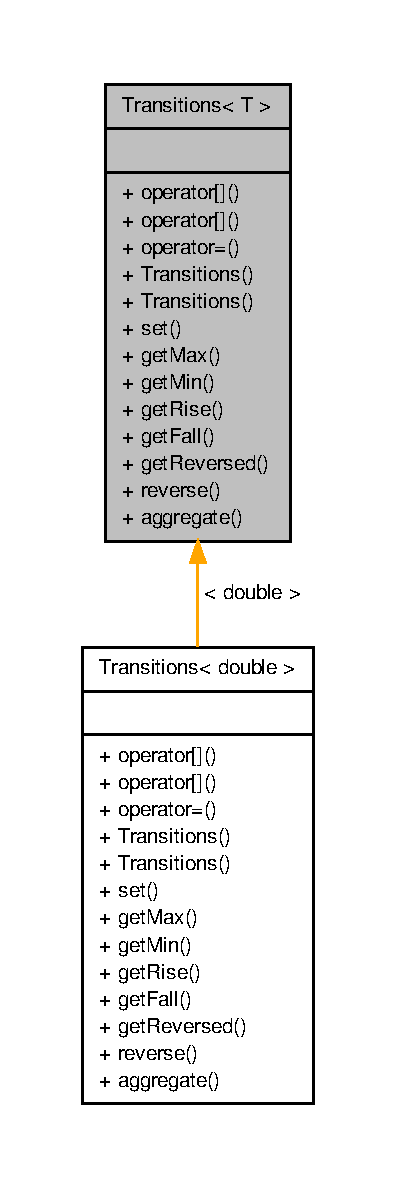
\includegraphics[height=550pt]{classTransitions__inherit__graph}
\end{center}
\end{figure}


Collaboration diagram for Transitions$<$ T $>$\-:\nopagebreak
\begin{figure}[H]
\begin{center}
\leavevmode
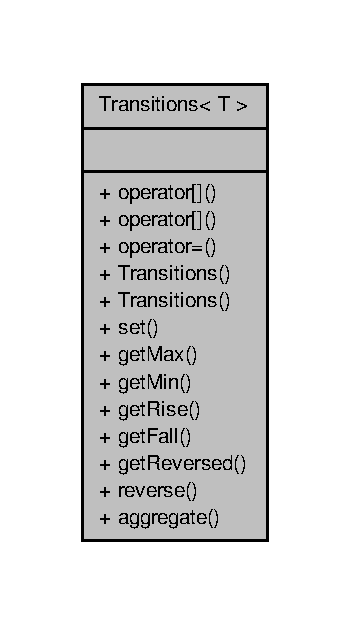
\includegraphics[width=168pt]{classTransitions__coll__graph}
\end{center}
\end{figure}
\subsection*{Public Member Functions}
\begin{DoxyCompactItemize}
\item 
T \& \hyperlink{classTransitions_a79a4be6a8415710583c6c811a27c3b9d}{operator\mbox{[}$\,$\mbox{]}} (const \hyperlink{transitions_8h_a424a64da753a3cd5e96ab8d0553a04c4}{Edge\-Type} edge\-Type)
\begin{DoxyCompactList}\small\item\em Refefinition of \mbox{[}\mbox{]} operator. Returns value of edge\-Type. \end{DoxyCompactList}\item 
T \hyperlink{classTransitions_af9dddcc4c48658b8adf8739ac139c34f}{operator\mbox{[}$\,$\mbox{]}} (const \hyperlink{transitions_8h_a424a64da753a3cd5e96ab8d0553a04c4}{Edge\-Type} edge\-Type) const 
\begin{DoxyCompactList}\small\item\em Refefinition of \mbox{[}\mbox{]} operator. Returns value of edge\-Type. \end{DoxyCompactList}\item 
\hyperlink{classTransitions}{Transitions} \& \hyperlink{classTransitions_a280ca4245034d6f298935392f8172cea}{operator=} (const \hyperlink{classTransitions}{Transitions} \&array)
\begin{DoxyCompactList}\small\item\em Refefinition of = operator. Sets caller transition time values to array time values and returns a pointer to it. \end{DoxyCompactList}\item 
\hyperlink{classTransitions_a0aae6de65968e98353b1fd9b6f394221}{Transitions} (const T rise, const T fall)
\begin{DoxyCompactList}\small\item\em \hyperlink{classTransitions}{Transitions} default constructor. \end{DoxyCompactList}\item 
\hyperlink{classTransitions_a5eb22fbf6b9a14410efc696742ee34df}{Transitions} ()
\begin{DoxyCompactList}\small\item\em Empty \hyperlink{classTransitions}{Transitions} constructor. \end{DoxyCompactList}\item 
void \hyperlink{classTransitions_aa237e34f678bd0aae62be692dc4059dc}{set} (const T rise, const T fall)
\begin{DoxyCompactList}\small\item\em Sets rise and fall time values. \end{DoxyCompactList}\item 
T \hyperlink{classTransitions_a59e47d34d366733da94f784c0177f8d9}{get\-Max} () const 
\begin{DoxyCompactList}\small\item\em Returns max value between rise and fall time. \end{DoxyCompactList}\item 
T \hyperlink{classTransitions_a37bb8749642ad21d22b264f39003d2ce}{get\-Min} () const 
\begin{DoxyCompactList}\small\item\em Returns min value between rise and fall time. \end{DoxyCompactList}\item 
T \hyperlink{classTransitions_ad88835ca81b7008ecfb7824bc5c17045}{get\-Rise} () const 
\begin{DoxyCompactList}\small\item\em Returns rise time value. \end{DoxyCompactList}\item 
T \hyperlink{classTransitions_affdb33e440b6ac3e6e685d83d46b3189}{get\-Fall} () const 
\begin{DoxyCompactList}\small\item\em Returns fall time value. \end{DoxyCompactList}\item 
\hyperlink{classTransitions}{Transitions}$<$ T $>$ \hyperlink{classTransitions_ac6e5a9efd02d3da3751fcaa845c7955b}{get\-Reversed} () const 
\begin{DoxyCompactList}\small\item\em Returns \hyperlink{classTransitions}{Transitions} with exchanged value. Ex\-: If called by Transitions$<$rise, fall$>$, returns Transitions$<$fall, rise$>$ \end{DoxyCompactList}\item 
void \hyperlink{classTransitions_ae547df9c8b8d6191aa95ca8f3e850605}{reverse} ()
\begin{DoxyCompactList}\small\item\em Exchanges rise and fall time values. Ex\-: Transitions$<$rise, fall$>$ becomes Transitions$<$fall, rise$>$ \end{DoxyCompactList}\item 
T \hyperlink{classTransitions_ab89e328a131f4ccf8882c67a30d6726c}{aggregate} () const 
\begin{DoxyCompactList}\small\item\em Returns the sum of rise and fall time values. \end{DoxyCompactList}\end{DoxyCompactItemize}
\subsection*{Friends}
\begin{DoxyCompactItemize}
\item 
ostream \& \hyperlink{classTransitions_a1f38245bca1673c266b44e9e2107c13d}{operator$<$$<$} (ostream \&out, const \hyperlink{classTransitions}{Transitions}$<$ T $>$ array)
\begin{DoxyCompactList}\small\item\em Redefinition of $<$$<$ operator. Inserts formatted description including rise and fall times, in this order. \end{DoxyCompactList}\item 
\hyperlink{classTransitions}{Transitions}$<$ T $>$ \hyperlink{classTransitions_af72b4da733791d7d350ed72162d8ea0f}{max} (const \hyperlink{classTransitions}{Transitions}$<$ T $>$ v0, const \hyperlink{classTransitions}{Transitions}$<$ T $>$ v1)
\begin{DoxyCompactList}\small\item\em Definition of max operator. Returns Transition$<$\-T$>$ with the higher values for rise and fall transition times. \end{DoxyCompactList}\item 
\hyperlink{classTransitions}{Transitions}$<$ T $>$ \hyperlink{classTransitions_aff6065ed38f85bcd39d2c2f8ce45f1d9}{min} (const \hyperlink{classTransitions}{Transitions}$<$ T $>$ v0, const \hyperlink{classTransitions}{Transitions}$<$ T $>$ v1)
\begin{DoxyCompactList}\small\item\em Definition of min operator. Returns Transition$<$\-T$>$ with the lower values for rise and fall transition times. \end{DoxyCompactList}\item 
\hyperlink{classTransitions}{Transitions}$<$ T $>$ \hyperlink{classTransitions_a3b968e944feed8bcb98aa1e6286fe175}{abs} (const \hyperlink{classTransitions}{Transitions}$<$ T $>$ v)
\begin{DoxyCompactList}\small\item\em Definition of abs operator. Returns Transition$<$\-T$>$ with the absolute values in I\-E\-E\-E floating point representation of rise and fall transition times. \end{DoxyCompactList}\item 
\hyperlink{classTransitions}{Transitions}$<$ T $>$ \hyperlink{classTransitions_a34f2a85ed601558365305cdcab645914}{pow} (const \hyperlink{classTransitions}{Transitions}$<$ T $>$ v, const double \hyperlink{classTransitions_ac02e6f8b007f44d55ed6b202c18ac0f8}{exp})
\begin{DoxyCompactList}\small\item\em Definition of pow operator. Returns Transition$<$\-T$>$ with rise and fall transition time values raised to exp. \end{DoxyCompactList}\item 
\hyperlink{classTransitions}{Transitions}$<$ T $>$ \hyperlink{classTransitions_aba9a3cd675e2077b57456b6ff699660d}{sqrt} (const \hyperlink{classTransitions}{Transitions}$<$ T $>$ v)
\begin{DoxyCompactList}\small\item\em Definition of abs operator. Returns Transition$<$\-T$>$ with the square root values of rise and fall transition times. \end{DoxyCompactList}\item 
\hyperlink{classTransitions}{Transitions}$<$ T $>$ \hyperlink{classTransitions_ac02e6f8b007f44d55ed6b202c18ac0f8}{exp} (const \hyperlink{classTransitions}{Transitions}$<$ T $>$ v)
\begin{DoxyCompactList}\small\item\em Definition of abs operator. Returns Transition$<$\-T$>$ with rise and fall transition time values in the form\-: $<$e$^\wedge$(rise time), e$^\wedge$(fall time)$>$, where 'e' is the Euler number e=2.\-718... \end{DoxyCompactList}\end{DoxyCompactItemize}


\subsection{Detailed Description}
\subsubsection*{template$<$typename T$>$class Transitions$<$ T $>$}

Template class which encapsulates any \mbox{[}rise,fall\mbox{]} twosome values and provides methods to work with it. 

\subsection{Constructor \& Destructor Documentation}
\hypertarget{classTransitions_a0aae6de65968e98353b1fd9b6f394221}{\index{Transitions@{Transitions}!Transitions@{Transitions}}
\index{Transitions@{Transitions}!Transitions@{Transitions}}
\subsubsection[{Transitions}]{\setlength{\rightskip}{0pt plus 5cm}template$<$typename T$>$ {\bf Transitions}$<$ T $>$\-::{\bf Transitions} (
\begin{DoxyParamCaption}
\item[{const T}]{rise, }
\item[{const T}]{fall}
\end{DoxyParamCaption}
)\hspace{0.3cm}{\ttfamily [inline]}}}\label{classTransitions_a0aae6de65968e98353b1fd9b6f394221}


\hyperlink{classTransitions}{Transitions} default constructor. 


\begin{DoxyParams}{Parameters}
{\em const} & T rise, const T fall \\
\hline
\end{DoxyParams}
\hypertarget{classTransitions_a5eb22fbf6b9a14410efc696742ee34df}{\index{Transitions@{Transitions}!Transitions@{Transitions}}
\index{Transitions@{Transitions}!Transitions@{Transitions}}
\subsubsection[{Transitions}]{\setlength{\rightskip}{0pt plus 5cm}template$<$typename T$>$ {\bf Transitions}$<$ T $>$\-::{\bf Transitions} (
\begin{DoxyParamCaption}
{}
\end{DoxyParamCaption}
)\hspace{0.3cm}{\ttfamily [inline]}}}\label{classTransitions_a5eb22fbf6b9a14410efc696742ee34df}


Empty \hyperlink{classTransitions}{Transitions} constructor. 



Here is the caller graph for this function\-:\nopagebreak
\begin{figure}[H]
\begin{center}
\leavevmode
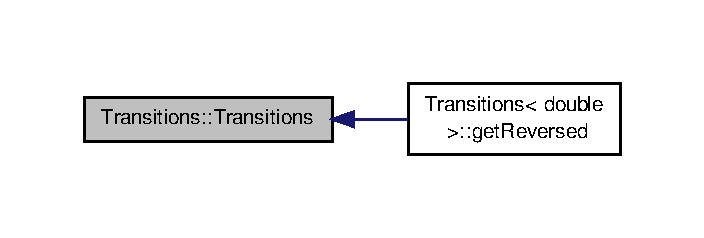
\includegraphics[width=338pt]{classTransitions_a5eb22fbf6b9a14410efc696742ee34df_icgraph}
\end{center}
\end{figure}




\subsection{Member Function Documentation}
\hypertarget{classTransitions_ab89e328a131f4ccf8882c67a30d6726c}{\index{Transitions@{Transitions}!aggregate@{aggregate}}
\index{aggregate@{aggregate}!Transitions@{Transitions}}
\subsubsection[{aggregate}]{\setlength{\rightskip}{0pt plus 5cm}template$<$typename T$>$ T {\bf Transitions}$<$ T $>$\-::aggregate (
\begin{DoxyParamCaption}
{}
\end{DoxyParamCaption}
) const\hspace{0.3cm}{\ttfamily [inline]}}}\label{classTransitions_ab89e328a131f4ccf8882c67a30d6726c}


Returns the sum of rise and fall time values. 

\begin{DoxyReturn}{Returns}
T 
\end{DoxyReturn}
\hypertarget{classTransitions_affdb33e440b6ac3e6e685d83d46b3189}{\index{Transitions@{Transitions}!get\-Fall@{get\-Fall}}
\index{get\-Fall@{get\-Fall}!Transitions@{Transitions}}
\subsubsection[{get\-Fall}]{\setlength{\rightskip}{0pt plus 5cm}template$<$typename T$>$ T {\bf Transitions}$<$ T $>$\-::get\-Fall (
\begin{DoxyParamCaption}
{}
\end{DoxyParamCaption}
) const\hspace{0.3cm}{\ttfamily [inline]}}}\label{classTransitions_affdb33e440b6ac3e6e685d83d46b3189}


Returns fall time value. 

\begin{DoxyReturn}{Returns}
T 
\end{DoxyReturn}


Here is the caller graph for this function\-:\nopagebreak
\begin{figure}[H]
\begin{center}
\leavevmode
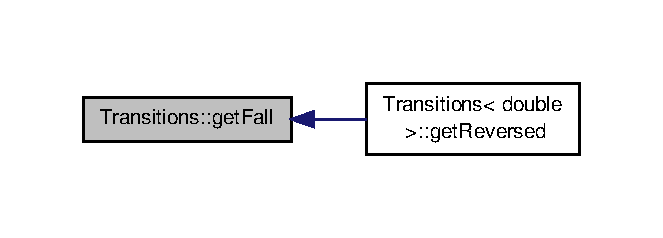
\includegraphics[width=318pt]{classTransitions_affdb33e440b6ac3e6e685d83d46b3189_icgraph}
\end{center}
\end{figure}


\hypertarget{classTransitions_a59e47d34d366733da94f784c0177f8d9}{\index{Transitions@{Transitions}!get\-Max@{get\-Max}}
\index{get\-Max@{get\-Max}!Transitions@{Transitions}}
\subsubsection[{get\-Max}]{\setlength{\rightskip}{0pt plus 5cm}template$<$typename T$>$ T {\bf Transitions}$<$ T $>$\-::get\-Max (
\begin{DoxyParamCaption}
{}
\end{DoxyParamCaption}
) const\hspace{0.3cm}{\ttfamily [inline]}}}\label{classTransitions_a59e47d34d366733da94f784c0177f8d9}


Returns max value between rise and fall time. 

\begin{DoxyReturn}{Returns}
T 
\end{DoxyReturn}
\hypertarget{classTransitions_a37bb8749642ad21d22b264f39003d2ce}{\index{Transitions@{Transitions}!get\-Min@{get\-Min}}
\index{get\-Min@{get\-Min}!Transitions@{Transitions}}
\subsubsection[{get\-Min}]{\setlength{\rightskip}{0pt plus 5cm}template$<$typename T$>$ T {\bf Transitions}$<$ T $>$\-::get\-Min (
\begin{DoxyParamCaption}
{}
\end{DoxyParamCaption}
) const\hspace{0.3cm}{\ttfamily [inline]}}}\label{classTransitions_a37bb8749642ad21d22b264f39003d2ce}


Returns min value between rise and fall time. 

\begin{DoxyReturn}{Returns}
T 
\end{DoxyReturn}
\hypertarget{classTransitions_ac6e5a9efd02d3da3751fcaa845c7955b}{\index{Transitions@{Transitions}!get\-Reversed@{get\-Reversed}}
\index{get\-Reversed@{get\-Reversed}!Transitions@{Transitions}}
\subsubsection[{get\-Reversed}]{\setlength{\rightskip}{0pt plus 5cm}template$<$typename T$>$ {\bf Transitions}$<$T$>$ {\bf Transitions}$<$ T $>$\-::get\-Reversed (
\begin{DoxyParamCaption}
{}
\end{DoxyParamCaption}
) const\hspace{0.3cm}{\ttfamily [inline]}}}\label{classTransitions_ac6e5a9efd02d3da3751fcaa845c7955b}


Returns \hyperlink{classTransitions}{Transitions} with exchanged value. Ex\-: If called by Transitions$<$rise, fall$>$, returns Transitions$<$fall, rise$>$ 

\begin{DoxyReturn}{Returns}
Transitions$<$\-T$>$ 
\end{DoxyReturn}
\hypertarget{classTransitions_ad88835ca81b7008ecfb7824bc5c17045}{\index{Transitions@{Transitions}!get\-Rise@{get\-Rise}}
\index{get\-Rise@{get\-Rise}!Transitions@{Transitions}}
\subsubsection[{get\-Rise}]{\setlength{\rightskip}{0pt plus 5cm}template$<$typename T$>$ T {\bf Transitions}$<$ T $>$\-::get\-Rise (
\begin{DoxyParamCaption}
{}
\end{DoxyParamCaption}
) const\hspace{0.3cm}{\ttfamily [inline]}}}\label{classTransitions_ad88835ca81b7008ecfb7824bc5c17045}


Returns rise time value. 

\begin{DoxyReturn}{Returns}
T 
\end{DoxyReturn}


Here is the caller graph for this function\-:\nopagebreak
\begin{figure}[H]
\begin{center}
\leavevmode
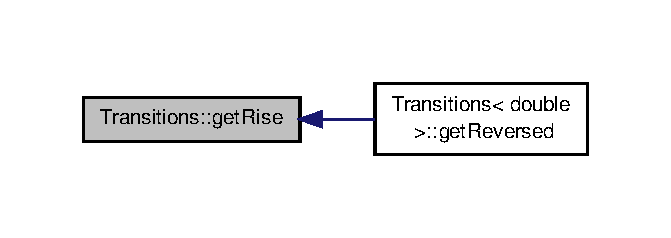
\includegraphics[width=322pt]{classTransitions_ad88835ca81b7008ecfb7824bc5c17045_icgraph}
\end{center}
\end{figure}


\hypertarget{classTransitions_a280ca4245034d6f298935392f8172cea}{\index{Transitions@{Transitions}!operator=@{operator=}}
\index{operator=@{operator=}!Transitions@{Transitions}}
\subsubsection[{operator=}]{\setlength{\rightskip}{0pt plus 5cm}template$<$typename T$>$ {\bf Transitions}\& {\bf Transitions}$<$ T $>$\-::operator= (
\begin{DoxyParamCaption}
\item[{const {\bf Transitions}$<$ T $>$ \&}]{array}
\end{DoxyParamCaption}
)\hspace{0.3cm}{\ttfamily [inline]}}}\label{classTransitions_a280ca4245034d6f298935392f8172cea}


Refefinition of = operator. Sets caller transition time values to array time values and returns a pointer to it. 


\begin{DoxyParams}{Parameters}
{\em const} & \hyperlink{classTransitions}{Transitions} \& array \\
\hline
\end{DoxyParams}
\hypertarget{classTransitions_a79a4be6a8415710583c6c811a27c3b9d}{\index{Transitions@{Transitions}!operator\mbox{[}$\,$\mbox{]}@{operator[]}}
\index{operator\mbox{[}$\,$\mbox{]}@{operator[]}!Transitions@{Transitions}}
\subsubsection[{operator[]}]{\setlength{\rightskip}{0pt plus 5cm}template$<$typename T$>$ T\& {\bf Transitions}$<$ T $>$\-::operator\mbox{[}$\,$\mbox{]} (
\begin{DoxyParamCaption}
\item[{const {\bf Edge\-Type}}]{edge\-Type}
\end{DoxyParamCaption}
)\hspace{0.3cm}{\ttfamily [inline]}}}\label{classTransitions_a79a4be6a8415710583c6c811a27c3b9d}


Refefinition of \mbox{[}\mbox{]} operator. Returns value of edge\-Type. 


\begin{DoxyParams}{Parameters}
{\em const} & Edge\-Type edge\-Type \\
\hline
\end{DoxyParams}
\hypertarget{classTransitions_af9dddcc4c48658b8adf8739ac139c34f}{\index{Transitions@{Transitions}!operator\mbox{[}$\,$\mbox{]}@{operator[]}}
\index{operator\mbox{[}$\,$\mbox{]}@{operator[]}!Transitions@{Transitions}}
\subsubsection[{operator[]}]{\setlength{\rightskip}{0pt plus 5cm}template$<$typename T$>$ T {\bf Transitions}$<$ T $>$\-::operator\mbox{[}$\,$\mbox{]} (
\begin{DoxyParamCaption}
\item[{const {\bf Edge\-Type}}]{edge\-Type}
\end{DoxyParamCaption}
) const\hspace{0.3cm}{\ttfamily [inline]}}}\label{classTransitions_af9dddcc4c48658b8adf8739ac139c34f}


Refefinition of \mbox{[}\mbox{]} operator. Returns value of edge\-Type. 


\begin{DoxyParams}{Parameters}
{\em const} & Edge\-Type edge\-Type \\
\hline
\end{DoxyParams}
\hypertarget{classTransitions_ae547df9c8b8d6191aa95ca8f3e850605}{\index{Transitions@{Transitions}!reverse@{reverse}}
\index{reverse@{reverse}!Transitions@{Transitions}}
\subsubsection[{reverse}]{\setlength{\rightskip}{0pt plus 5cm}template$<$typename T$>$ void {\bf Transitions}$<$ T $>$\-::reverse (
\begin{DoxyParamCaption}
{}
\end{DoxyParamCaption}
)\hspace{0.3cm}{\ttfamily [inline]}}}\label{classTransitions_ae547df9c8b8d6191aa95ca8f3e850605}


Exchanges rise and fall time values. Ex\-: Transitions$<$rise, fall$>$ becomes Transitions$<$fall, rise$>$ 

\begin{DoxyReturn}{Returns}
T 
\end{DoxyReturn}
\hypertarget{classTransitions_aa237e34f678bd0aae62be692dc4059dc}{\index{Transitions@{Transitions}!set@{set}}
\index{set@{set}!Transitions@{Transitions}}
\subsubsection[{set}]{\setlength{\rightskip}{0pt plus 5cm}template$<$typename T$>$ void {\bf Transitions}$<$ T $>$\-::set (
\begin{DoxyParamCaption}
\item[{const T}]{rise, }
\item[{const T}]{fall}
\end{DoxyParamCaption}
)\hspace{0.3cm}{\ttfamily [inline]}}}\label{classTransitions_aa237e34f678bd0aae62be692dc4059dc}


Sets rise and fall time values. 


\begin{DoxyParams}{Parameters}
{\em const} & T rise, const T fall\\
\hline
\end{DoxyParams}
\begin{DoxyReturn}{Returns}
void 
\end{DoxyReturn}


\subsection{Friends And Related Function Documentation}
\hypertarget{classTransitions_a3b968e944feed8bcb98aa1e6286fe175}{\index{Transitions@{Transitions}!abs@{abs}}
\index{abs@{abs}!Transitions@{Transitions}}
\subsubsection[{abs}]{\setlength{\rightskip}{0pt plus 5cm}template$<$typename T$>$ {\bf Transitions}$<$T$>$ abs (
\begin{DoxyParamCaption}
\item[{const {\bf Transitions}$<$ T $>$}]{v}
\end{DoxyParamCaption}
)\hspace{0.3cm}{\ttfamily [friend]}}}\label{classTransitions_a3b968e944feed8bcb98aa1e6286fe175}


Definition of abs operator. Returns Transition$<$\-T$>$ with the absolute values in I\-E\-E\-E floating point representation of rise and fall transition times. 


\begin{DoxyParams}{Parameters}
{\em const} & Transitions$<$\-T$>$ v\\
\hline
\end{DoxyParams}
\begin{DoxyReturn}{Returns}
Transition$<$\-T$>$ 
\end{DoxyReturn}
\hypertarget{classTransitions_ac02e6f8b007f44d55ed6b202c18ac0f8}{\index{Transitions@{Transitions}!exp@{exp}}
\index{exp@{exp}!Transitions@{Transitions}}
\subsubsection[{exp}]{\setlength{\rightskip}{0pt plus 5cm}template$<$typename T$>$ {\bf Transitions}$<$T$>$ exp (
\begin{DoxyParamCaption}
\item[{const {\bf Transitions}$<$ T $>$}]{v}
\end{DoxyParamCaption}
)\hspace{0.3cm}{\ttfamily [friend]}}}\label{classTransitions_ac02e6f8b007f44d55ed6b202c18ac0f8}


Definition of abs operator. Returns Transition$<$\-T$>$ with rise and fall transition time values in the form\-: $<$e$^\wedge$(rise time), e$^\wedge$(fall time)$>$, where 'e' is the Euler number e=2.\-718... 


\begin{DoxyParams}{Parameters}
{\em const} & Transitions$<$\-T$>$ v\\
\hline
\end{DoxyParams}
\begin{DoxyReturn}{Returns}
Transition$<$\-T$>$ 
\end{DoxyReturn}
\hypertarget{classTransitions_af72b4da733791d7d350ed72162d8ea0f}{\index{Transitions@{Transitions}!max@{max}}
\index{max@{max}!Transitions@{Transitions}}
\subsubsection[{max}]{\setlength{\rightskip}{0pt plus 5cm}template$<$typename T$>$ {\bf Transitions}$<$T$>$ max (
\begin{DoxyParamCaption}
\item[{const {\bf Transitions}$<$ T $>$}]{v0, }
\item[{const {\bf Transitions}$<$ T $>$}]{v1}
\end{DoxyParamCaption}
)\hspace{0.3cm}{\ttfamily [friend]}}}\label{classTransitions_af72b4da733791d7d350ed72162d8ea0f}


Definition of max operator. Returns Transition$<$\-T$>$ with the higher values for rise and fall transition times. 


\begin{DoxyParams}{Parameters}
{\em const} & Transitions$<$\-T$>$ v0\\
\hline
\end{DoxyParams}
\begin{DoxyReturn}{Returns}
Transition$<$\-T$>$ 
\end{DoxyReturn}
\hypertarget{classTransitions_aff6065ed38f85bcd39d2c2f8ce45f1d9}{\index{Transitions@{Transitions}!min@{min}}
\index{min@{min}!Transitions@{Transitions}}
\subsubsection[{min}]{\setlength{\rightskip}{0pt plus 5cm}template$<$typename T$>$ {\bf Transitions}$<$T$>$ min (
\begin{DoxyParamCaption}
\item[{const {\bf Transitions}$<$ T $>$}]{v0, }
\item[{const {\bf Transitions}$<$ T $>$}]{v1}
\end{DoxyParamCaption}
)\hspace{0.3cm}{\ttfamily [friend]}}}\label{classTransitions_aff6065ed38f85bcd39d2c2f8ce45f1d9}


Definition of min operator. Returns Transition$<$\-T$>$ with the lower values for rise and fall transition times. 


\begin{DoxyParams}{Parameters}
{\em const} & Transitions$<$\-T$>$ v0, const Transitions$<$\-T$>$ v1\\
\hline
\end{DoxyParams}
\begin{DoxyReturn}{Returns}
Transition$<$\-T$>$ 
\end{DoxyReturn}
\hypertarget{classTransitions_a1f38245bca1673c266b44e9e2107c13d}{\index{Transitions@{Transitions}!operator$<$$<$@{operator$<$$<$}}
\index{operator$<$$<$@{operator$<$$<$}!Transitions@{Transitions}}
\subsubsection[{operator$<$$<$}]{\setlength{\rightskip}{0pt plus 5cm}template$<$typename T$>$ ostream\& operator$<$$<$ (
\begin{DoxyParamCaption}
\item[{ostream \&}]{out, }
\item[{const {\bf Transitions}$<$ T $>$}]{array}
\end{DoxyParamCaption}
)\hspace{0.3cm}{\ttfamily [friend]}}}\label{classTransitions_a1f38245bca1673c266b44e9e2107c13d}


Redefinition of $<$$<$ operator. Inserts formatted description including rise and fall times, in this order. 


\begin{DoxyParams}{Parameters}
{\em ostream} & \&out, const Transitions$<$\-T$>$ array \\
\hline
\end{DoxyParams}
\hypertarget{classTransitions_a34f2a85ed601558365305cdcab645914}{\index{Transitions@{Transitions}!pow@{pow}}
\index{pow@{pow}!Transitions@{Transitions}}
\subsubsection[{pow}]{\setlength{\rightskip}{0pt plus 5cm}template$<$typename T$>$ {\bf Transitions}$<$T$>$ pow (
\begin{DoxyParamCaption}
\item[{const {\bf Transitions}$<$ T $>$}]{v, }
\item[{const double}]{exp}
\end{DoxyParamCaption}
)\hspace{0.3cm}{\ttfamily [friend]}}}\label{classTransitions_a34f2a85ed601558365305cdcab645914}


Definition of pow operator. Returns Transition$<$\-T$>$ with rise and fall transition time values raised to exp. 


\begin{DoxyParams}{Parameters}
{\em const} & Transitions$<$\-T$>$ v, const double exp\\
\hline
\end{DoxyParams}
\begin{DoxyReturn}{Returns}
Transition$<$\-T$>$ 
\end{DoxyReturn}
\hypertarget{classTransitions_aba9a3cd675e2077b57456b6ff699660d}{\index{Transitions@{Transitions}!sqrt@{sqrt}}
\index{sqrt@{sqrt}!Transitions@{Transitions}}
\subsubsection[{sqrt}]{\setlength{\rightskip}{0pt plus 5cm}template$<$typename T$>$ {\bf Transitions}$<$T$>$ sqrt (
\begin{DoxyParamCaption}
\item[{const {\bf Transitions}$<$ T $>$}]{v}
\end{DoxyParamCaption}
)\hspace{0.3cm}{\ttfamily [friend]}}}\label{classTransitions_aba9a3cd675e2077b57456b6ff699660d}


Definition of abs operator. Returns Transition$<$\-T$>$ with the square root values of rise and fall transition times. 


\begin{DoxyParams}{Parameters}
{\em const} & Transitions$<$\-T$>$ v\\
\hline
\end{DoxyParams}
\begin{DoxyReturn}{Returns}
Transition$<$\-T$>$ 
\end{DoxyReturn}


The documentation for this class was generated from the following file\-:\begin{DoxyCompactItemize}
\item 
Timing\-Analysis/src/include/\hyperlink{transitions_8h}{transitions.\-h}\end{DoxyCompactItemize}

\hypertarget{classVerilogParser}{\section{Verilog\-Parser Class Reference}
\label{classVerilogParser}\index{Verilog\-Parser@{Verilog\-Parser}}
}


Inherits from \hyperlink{classParser}{Parser}. Parse verilog files. Used to generate circuit netlists.  




{\ttfamily \#include $<$parser.\-h$>$}



Inheritance diagram for Verilog\-Parser\-:\nopagebreak
\begin{figure}[H]
\begin{center}
\leavevmode
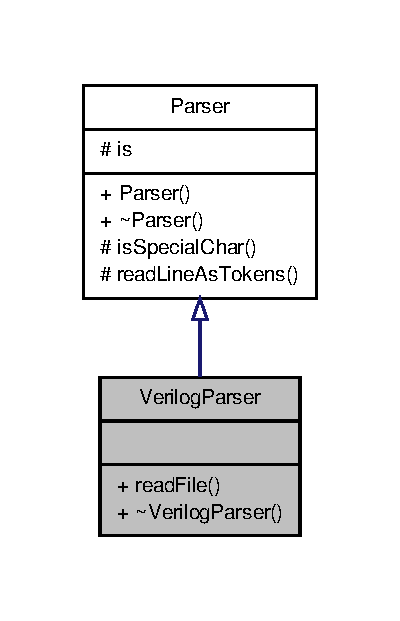
\includegraphics[width=192pt]{classVerilogParser__inherit__graph}
\end{center}
\end{figure}


Collaboration diagram for Verilog\-Parser\-:\nopagebreak
\begin{figure}[H]
\begin{center}
\leavevmode
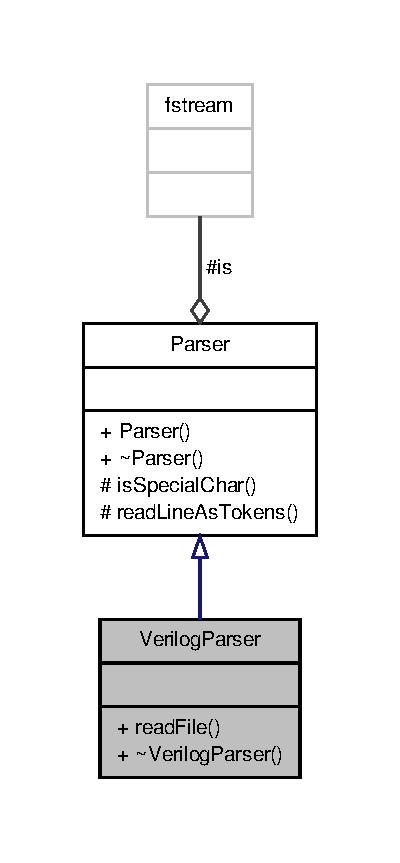
\includegraphics[width=192pt]{classVerilogParser__coll__graph}
\end{center}
\end{figure}
\subsection*{Public Member Functions}
\begin{DoxyCompactItemize}
\item 
const \hyperlink{classCircuit__Netlist}{Circuit\-\_\-\-Netlist} \hyperlink{classVerilogParser_a9f8740c184e8129a87597a1eae3ed3c4}{read\-File} (const string filename)
\begin{DoxyCompactList}\small\item\em Returns \hyperlink{classCircuit__Netlist}{Circuit\-\_\-\-Netlist} object generated by information read from file passed as filename parameter. \end{DoxyCompactList}\item 
virtual \hyperlink{classVerilogParser_aee565da994b012a04f4d7120b9148ab3}{$\sim$\-Verilog\-Parser} ()
\begin{DoxyCompactList}\small\item\em Empty \hyperlink{classVerilogParser}{Verilog\-Parser} destructor. \end{DoxyCompactList}\end{DoxyCompactItemize}
\subsection*{Additional Inherited Members}


\subsection{Detailed Description}
Inherits from \hyperlink{classParser}{Parser}. Parse verilog files. Used to generate circuit netlists. 

\subsection{Constructor \& Destructor Documentation}
\hypertarget{classVerilogParser_aee565da994b012a04f4d7120b9148ab3}{\index{Verilog\-Parser@{Verilog\-Parser}!$\sim$\-Verilog\-Parser@{$\sim$\-Verilog\-Parser}}
\index{$\sim$\-Verilog\-Parser@{$\sim$\-Verilog\-Parser}!VerilogParser@{Verilog\-Parser}}
\subsubsection[{$\sim$\-Verilog\-Parser}]{\setlength{\rightskip}{0pt plus 5cm}virtual Verilog\-Parser\-::$\sim$\-Verilog\-Parser (
\begin{DoxyParamCaption}
{}
\end{DoxyParamCaption}
)\hspace{0.3cm}{\ttfamily [inline]}, {\ttfamily [virtual]}}}\label{classVerilogParser_aee565da994b012a04f4d7120b9148ab3}


Empty \hyperlink{classVerilogParser}{Verilog\-Parser} destructor. 



\subsection{Member Function Documentation}
\hypertarget{classVerilogParser_a9f8740c184e8129a87597a1eae3ed3c4}{\index{Verilog\-Parser@{Verilog\-Parser}!read\-File@{read\-File}}
\index{read\-File@{read\-File}!VerilogParser@{Verilog\-Parser}}
\subsubsection[{read\-File}]{\setlength{\rightskip}{0pt plus 5cm}const {\bf Circuit\-\_\-\-Netlist} Verilog\-Parser\-::read\-File (
\begin{DoxyParamCaption}
\item[{const string}]{filename}
\end{DoxyParamCaption}
)}}\label{classVerilogParser_a9f8740c184e8129a87597a1eae3ed3c4}


Returns \hyperlink{classCircuit__Netlist}{Circuit\-\_\-\-Netlist} object generated by information read from file passed as filename parameter. 


\begin{DoxyParams}{Parameters}
{\em const} & string filename\\
\hline
\end{DoxyParams}
\begin{DoxyReturn}{Returns}
const \hyperlink{classCircuit__Netlist}{Circuit\-\_\-\-Netlist} 
\end{DoxyReturn}


The documentation for this class was generated from the following file\-:\begin{DoxyCompactItemize}
\item 
Timing\-Analysis/src/include/\hyperlink{parser_8h}{parser.\-h}\end{DoxyCompactItemize}

\hypertarget{classWireDelayModel}{\section{Wire\-Delay\-Model Class Reference}
\label{classWireDelayModel}\index{Wire\-Delay\-Model@{Wire\-Delay\-Model}}
}
Inheritance diagram for Wire\-Delay\-Model\-:\begin{figure}[H]
\begin{center}
\leavevmode
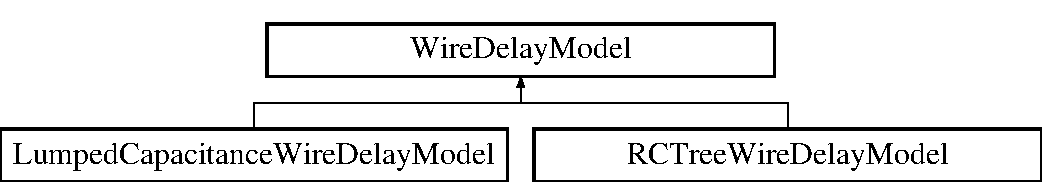
\includegraphics[height=2.000000cm]{classWireDelayModel}
\end{center}
\end{figure}
\subsection*{Public Member Functions}
\begin{DoxyCompactItemize}
\item 
\hypertarget{classWireDelayModel_a0fd2defb581f6d8bcd67e5c935387d95}{{\bfseries Wire\-Delay\-Model} (const double \&lumped\-\_\-capacitance)}\label{classWireDelayModel_a0fd2defb581f6d8bcd67e5c935387d95}

\item 
\hypertarget{classWireDelayModel_a8375f713365be98c03672dbeb28eb930}{virtual const \hyperlink{classTransitions}{Transitions}$<$ double $>$ {\bfseries simulate} (const \hyperlink{structLibertyCellInfo}{Liberty\-Cell\-Info} \&cell\-Info, const int input, const \hyperlink{classTransitions}{Transitions}$<$ double $>$ slew, bool is\-\_\-input\-\_\-driver)=0}\label{classWireDelayModel_a8375f713365be98c03672dbeb28eb930}

\item 
\hypertarget{classWireDelayModel_a45a83dd192bcbf2a70ee13899256fe0d}{virtual const \hyperlink{classTransitions}{Transitions}$<$ double $>$ {\bfseries delay\-\_\-at\-\_\-fanout\-\_\-node} (const string fanout\-\_\-node\-\_\-name) const =0}\label{classWireDelayModel_a45a83dd192bcbf2a70ee13899256fe0d}

\item 
\hypertarget{classWireDelayModel_adaf486017e2ad91a900a9bef4e6f9340}{virtual const \hyperlink{classTransitions}{Transitions}$<$ double $>$ {\bfseries slew\-\_\-at\-\_\-fanout\-\_\-node} (const string fanout\-\_\-node\-\_\-name) const =0}\label{classWireDelayModel_adaf486017e2ad91a900a9bef4e6f9340}

\item 
\hypertarget{classWireDelayModel_a27d557bc1f2ed7e5e9787a8a5d82ecb2}{virtual void {\bfseries set\-Fanout\-Pin\-Capacitance} (const string fanout\-Name\-And\-Pin, const double pin\-Capacitance)=0}\label{classWireDelayModel_a27d557bc1f2ed7e5e9787a8a5d82ecb2}

\item 
\hypertarget{classWireDelayModel_a4f4ab93810af8ad90fd9fca0b06de141}{virtual \hyperlink{classTransitions}{Transitions}$<$ double $>$ {\bfseries root\-\_\-delay} (int arc\-\_\-number)=0}\label{classWireDelayModel_a4f4ab93810af8ad90fd9fca0b06de141}

\item 
\hypertarget{classWireDelayModel_a9e5344c26b73f549a2b5c38fea8af13d}{virtual \hyperlink{classTransitions}{Transitions}$<$ double $>$ {\bfseries root\-\_\-slew} (int arc\-\_\-number)=0}\label{classWireDelayModel_a9e5344c26b73f549a2b5c38fea8af13d}

\item 
\hypertarget{classWireDelayModel_a74869a3a66deb53507e8bc6f16eff45c}{virtual void {\bfseries clear} ()=0}\label{classWireDelayModel_a74869a3a66deb53507e8bc6f16eff45c}

\item 
\hypertarget{classWireDelayModel_a05f509843dfa07e17c9b6cc16ba9aaa0}{double {\bfseries lumped\-\_\-capacitance} () const }\label{classWireDelayModel_a05f509843dfa07e17c9b6cc16ba9aaa0}

\end{DoxyCompactItemize}
\subsection*{Protected Attributes}
\begin{DoxyCompactItemize}
\item 
\hypertarget{classWireDelayModel_ab03b1640710e81c9dcd4cbe9b7fed329}{double {\bfseries \-\_\-lumped\-\_\-capacitance}}\label{classWireDelayModel_ab03b1640710e81c9dcd4cbe9b7fed329}

\end{DoxyCompactItemize}
\subsection*{Static Protected Attributes}
\begin{DoxyCompactItemize}
\item 
\hypertarget{classWireDelayModel_aa8f767316492b902c13ec68651b30247}{static \\*
\hyperlink{classLinearLibertyLookupTableInterpolator}{Linear\-Liberty\-Lookup\-Table\-Interpolator} {\bfseries interpolator}}\label{classWireDelayModel_aa8f767316492b902c13ec68651b30247}

\end{DoxyCompactItemize}


The documentation for this class was generated from the following file\-:\begin{DoxyCompactItemize}
\item 
tcc\-Chrystian/src/include/wire\-\_\-delay\-\_\-model.\-h\end{DoxyCompactItemize}

%--- End generated contents ---

% Index
\newpage
\phantomsection
\addcontentsline{toc}{part}{Index}
\printindex

\end{document}
